\documentclass{book}[12pt]
\usepackage{times}

\usepackage{latexsym}
\usepackage{MnSymbol}
\usepackage{comment}
\usepackage{url}
\usepackage{fullpage}
\usepackage{scrextend}
\usepackage{proof}
\usepackage{array}
\usepackage{xspace}
\usepackage{stmaryrd}
\usepackage{graphicx}
\usepackage{amsmath,amsfonts,amsthm}
\usepackage{makeidx}
\usepackage{float}

\usepackage{tikz}
\usetikzlibrary{arrows}
\usetikzlibrary{shapes}

\usepackage{thmtools}
\declaretheorem[name=Theorem,shaded={},numberwithin=section]{theorem}
\declaretheorem[sibling=theorem]{definition}
\declaretheorem[sibling=theorem]{lemma}
\declaretheorem[sibling=theorem]{corollary}

\usepackage[pdftex,
	pdfauthor={Aaron Stump},
	pdftitle={Introduction to Lambda Calculus},
	colorlinks,
	urlcolor={blue},
	linkcolor={blue},
        citecolor={blue}]{hyperref}

% style for figures
\floatstyle{boxed}
\restylefloat{table}
\restylefloat{figure}


\makeindex

\begin{document}

\title{Introduction to Lambda Calculus}

\author{Aaron Stump \\
Computer Science \\
The University of Iowa
}

\maketitle
\frontmatter

\tableofcontents

\mainmatter

%%%%%%%%%%%%%%%%%%%%%%%%%%%%%%%%%%%%%%%%%%%%%%%%%%%%%%%%%%%%%%%%%%%%%%
% for definitions, proofs, etc.
%%%%%%%%%%%%%%%%%%%%%%%%%%%%%%%%%%%%%%%%%%%%%%%%%%%%%%%%%%%%%%%%%%%%%%

\newcommand{\paradef}[2]{\vspace{#1 cm} %
  \noindent %
  \textbf{#2}}

\newcommand{\case}[1]{\vspace{.1cm} %
  \noindent \underline{Case#1:}}

\newcommand{\todo}[1]{\textbf{[#1]}}

%%%%%%%%%%%%%%%%%%%%%%%%%%%%%%%%%%%%%%%%%%%%%%%%%%%%%%%%%%%%%%%%%%%%%%
% for beta
%%%%%%%%%%%%%%%%%%%%%%%%%%%%%%%%%%%%%%%%%%%%%%%%%%%%%%%%%%%%%%%%%%%%%%

\newcommand{\lam}[2]{\lambda\ #1.\, #2}

% arrows
\newcommand{\curva}[0]{\rightlsquigarrow}
\newcommand{\scurva}[0]{\squigarrowleftright}

% reduction relations
\newcommand{\betar}[0]{\curva_\beta}
\newcommand{\betaa}[0]{\curva}

\newcommand{\Tau}[0]{\mathcal{T}}

%%%%%%%%%%%%%%%%%%%%%%%%%%%%%%%%%%%%%%%%%%%%%%%%%%%%%%%%%%%%%%%%%%%%%%
% for lambda encodings
%%%%%%%%%%%%%%%%%%%%%%%%%%%%%%%%%%%%%%%%%%%%%%%%%%%%%%%%%%%%%%%%%%%%%%

\newcommand{\rep}[1]{\ulcorner #1 \urcorner}

%%%%%%%%%%%%%%%%%%%%%%%%%%%%%%%%%%%%%%%%%%%%%%%%%%%%%%%%%%%%%%%%%%%%%%
% for confluence
%%%%%%%%%%%%%%%%%%%%%%%%%%%%%%%%%%%%%%%%%%%%%%%%%%%%%%%%%%%%%%%%%%%%%%
\newcommand{\Pred}[0]{\Rightarrow}


%%%%%%%%%%%%%%%%%%%%%%%%%%%%%%%%%%%%%%%%%%%%%%%%%%%%%%%%%%%%%%%%%%%%%%
% for STLC
%%%%%%%%%%%%%%%%%%%%%%%%%%%%%%%%%%%%%%%%%%%%%%%%%%%%%%%%%%%%%%%%%%%%%%
\newcommand{\interp}[1]{\llbracket #1 \rrbracket}
\newcommand{\all}[2]{\forall\ #1.\, #2}


\part{Untyped Lambda Calculus}
\chapter{Introduction}

The formal system known as lambda calculus was invented by Alonzo
Church, and published first in his paper ``A Set of Postulates for the
Foundation of Logic''~\cite{church32}.  As that title suggests,
Church's motivation for devising lambda calculus was to create a
formal foundation for logic and mathematics.  This was in response to
the crisis in foundations of mathematics that occurred in the early
20th century, with the discovery of paradoxes in proposed foundational
theories.  Bertrand Russell's discovery, in 1901, of a contradiction
in the foundational theory being developed by Gottlob Frege was a
prime and motivating example~\cite{Whitehead:268025}.  Church's own
theory was quickly discovered to be inconsistent, as, sadly, was even
a revised version~\cite{church33}.  

One may take these failures as as a cautionary tale of the difficulty
of creating consistent foundational theories.  Or, more inspiringly,
one can understand them as showing that many good results can come
from endeavors that fall short of their objectives.  For from these
early systems of Church, and the work he and his brilliant graduate
students carried out consequently, has arisen a remarkable line of
inquiry, with tremendous theoretical and practical impact, on the
subjects of typed and untyped lambda calculus.  For an engaging
exposition of this history, see the paper by Cardone
and Hindley~\cite{cardone09}.

Church subsequently published a research monograph focused on the
lambda calculus as a formal notion of computation, rather than a
foundation for mathematics~\cite{church41}.  I will take this
monograph to be his definitive presentation of lambda calculus.

\subsection{Why this book}

There are a number of very impressive books on lambda calculus
currently available.  For example, Hendrik Barendregt's book remains
an authoritative source for many deep topics in the theory of untyped
lambda calculus~\cite{barendregt85}, and his more recent book,
co-authored with will Dekkers and Richard Statman, is a similar source
for certain topics in typed lambda calculus~\cite{barendregt+13}.  But
these are reference works, which are far too advanced to serve as
textbooks.  One book on lambda calculus that is at an appropriate
level for university instruction is the one by J. Roger Hindley and
Jonathan Seldin~\cite{hindley+08}.  But this book has a more
mathematical perspective on the subject, and puts less emphasis on
certain more computational points.  So in my opinion, there is
currently no available textbook, for students at the late
undergraduate or early graduate level, on lambda calculus from the
perspective of Computer Science.  And that is what the current
volume seeks to supply.

\chapter{Syntax and Reduction Semantics}

\section{The syntax of lambda terms}
\label{sec:synlam}

The untyped lambda calculus has a very small syntax, an appealing
quality for both theoretical study and practical use.  There are just
two syntactic categories: variables and terms.  We assume variables
are taken from some countably infinite set of mathematical objects
(like the natural numbers) disjoint from the other forms of term, and
generally avoid specifying them further.  One stipulation, though is
that whatever variables are, we should be able to test effectively
whether or not two variables are equal.  Such an equality test will be
needed when defining substitution.  We will use $x$ as a meta-variable
for variables, and adopt the convention that in any particular
meta-linguistic discussion, different such meta-variables refer to
different variables.  So if we write $x$ and $y$, please understand
that these meta-variables refer to different actual variables.

Terms are then certain labeled binary trees.  We will use the
meta-variable $t$ (and decorated versions like $t_1$, $t'$, etc.) for
terms.  They are either leaf nodes labeled with variables $x$,
application nodes with subtrees $t_1$ and $t_2$, or lambda nodes with
subtree labeled $x$ and subtree $t'$.  Pictorially, these are shown in
Figure~\ref{fig:lamtrees}.  An application node is said to apply
$t_1$, as a function, to $t_2$, as an argument to that function.  For
a lambda node with subtree labeled $x$ and subtree $t'$, the term $t'$
is called the \emph{body} of the $\lambda$-node.  A term whose root is
labeled $\lambda$ is called a $\lambda$-abstraction.  

\begin{figure}
\begin{center}
\large
\begin{tikzpicture}
  \node at (0,0) {\ }
    child {node {$x$} edge from parent[draw=none]};

  \node at (3,0) {@}
  child { node {$t_1$}}
  child { node {$t_2$}};

  \node at (6,0) {$\lambda$}
  child { node {$x$}}
  child { node {$t'$}};

\end{tikzpicture}
\end{center}
\caption{Graphical depiction of the syntax of terms $t$}
\label{fig:lamtrees}
\end{figure}

While understanding the tree structure for terms is essential for the
study of lambda calculus, it is typical to present terms not as trees,
but textually.  For this, we use the following context-free
grammar, together with two parsing conventions:
\[
\textit{terms}\ t\ ::=\ x\ |\ t_1\ t_2\ |\ \lam{x}{t}\ |\ ( t )
\]
\noindent The parsing conventions are:
\begin{enumerate}
\item Application is left-associative.  So $a\ b\ c$ should be interpreted as $(a\ b)\ c$, as opposed to $a\ (b\ c)$.
\item The scope of $\lambda\ x$ is as far to the right as possible.  So $\lam{x}{x\ x}$ should be interpreted as $\lam{x}{(x\ x)}$, because this grouping shows that the $\lambda\ x$ part of the term governs the application $x\ x$.  This disambiguation is used, instead of $(\lam{x}{x})\ x$.
\end{enumerate}
\noindent Parentheses are just used for disambiguation and do not
correspond to any node in the tree syntax (of
Figure~\ref{fig:lamtrees}).  Figure~\ref{fig:exampleterms} shows
several example terms in both textual form and tree form.  Exercises
below (Section~\ref{sec:extree}) require you to translate between
these forms for some other examples.

\begin{figure}
\large
\begin{center}
\begin{tabular}{llll}

\underline{Textual:} &
$\lam{x}{x}$ &
$x\ \lam{x}{x\ x}$ &
$\lam{x}{\lam{y}{y\ x\ x}}$

\\ 
\underline{Disambiguated:} &
$\lam{x}{x}$ &
$x\ \lam{x}{(x\ x)}$ &
$\lam{x}{\lam{y}{((y\ x) x)}}$

\\ 

\begin{tikzpicture}
  \node at (0,0) {\underline{Tree:}}
  child { node {\ } edge from parent[draw=none]
    child { node {\ } edge from parent[draw=none]
      child { node {\ } edge from parent[draw=none]
        child { node {\ } edge from parent[draw=none]}}}};
\end{tikzpicture}

\vspace{1cm}
&

\begin{tikzpicture}
  \node at (0,0) {$\lambda$}
  child { node {$x$}}
  child { node {$x$}
    child { node {\ } edge from parent[draw=none]
      child { node {\ } edge from parent[draw=none]
        child { node {\ } edge from parent[draw=none]
}}}};
\end{tikzpicture}

&

\begin{tikzpicture}
  \node at (0,0) {@}
  child { node {$x$}}
  child { node {$\lambda$}
    child { node {$x$}}
    child { node {@}
      child { node {$x$} }
      child { node {$x$}
      child { node {\ } edge from parent[draw=none]}}}};
\end{tikzpicture}

&

\begin{tikzpicture}
  \node at (0,0) {$\lambda$}
  child { node {$x$}}
  child { node {$\lambda$}
    child { node {$y$}}
    child { node {@}
      child { node {@}
        child {node {$y$}}
        child {node {$x$}}}
      child { node {$x$}}}};
\end{tikzpicture}

\\


\end{tabular}

\end{center}
\caption{Some example terms, in textual form (where parsing conventions must be applied), then disambiguated textual form (no parsing conventions needed), and finally tree form}
\label{fig:exampleterms}
\end{figure}

\begin{definition}[subterm]
  A subterm of a term $t$ is just some subtree (possibly $t$ itself) of $t$.\index{subterm}
  \end{definition}

\section{Binding, bound, and free variable occurrences}

As will become more apparent shortly, the $\lambda$ symbol introduces
its variable $x$ \emph{locally} in the body.  This means that this $x$
used in the body of a $\lambda$-abstraction is semantically different
from the same variable $x$ used outside the body.  In Computer Science
terms, $\lambda$ introduces $x$ as a local variable, whose scope
(i.e., the part of the expression where this variable introduction is
in force) is the body of the $\lambda$-abstraction.

The following basic terminology is used to describe occurrences of a
variable $x$; i.e., nodes in term (in tree form) labeled by a
variable.  If the occurrence is the left child of a $\lambda$-node,
then this is called a \emph{binding} occurrence\index{variable!binding
  occurrence}.  If the occurrence is somewhere inside the right
subtree of a $\lambda$-node introducing $x$, then the occurrence is
called \emph{bound}\index{variable!bound occurrence}.  And finally, if
the variable occurrence is neither binding nor bound it is called
\emph{free}\index{variable!free occurrence}: it is not in the scope of
a $\lambda$-node binding $x$.  It is common to write $\textit{FV}(t)$
for the set of variables with free occurrences in $t$\index{FV}.  See
Figure~\ref{fig:varocc} for an example illustrating this terminology.
A term with at least one free variable occurrence is called \emph{open}\index{term!open},
and a term with no free variable occurrences is called \emph{closed}\index{term!closed}.

\begin{figure}
\large
\begin{center}
    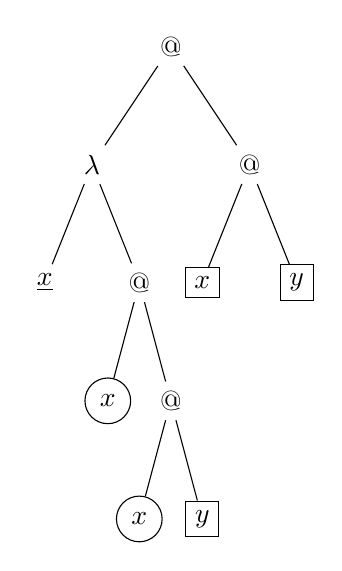
\begin{tikzpicture}
      [level 1/.style={sibling distance=20mm},
        level 2/.style={sibling distance=12mm},
          level 3/.style={sibling distance=8mm}]
      \node at (0,0) {@}
            child { node {$\lambda$}
              child { node {\underline{$x$}}}
              child { node {@}
                child { node [draw,circle] {$x$}}
                child { node {@}
                  child { node[draw,circle] {$x$}}
                  child { node[draw,rectangle] {$y$}}
}}}
            child { node {@}
              child {node[draw,rectangle] {$x$}}
              child {node[draw,rectangle] {$y$}}};
    \end{tikzpicture}
    \end{center}
    \caption{Example term illustrating the concepts of binding, bound, and free variable occurrence.  The underlined node is a binding occurrence, circled nodes are bound occurrences (bound by that sole underlined binding occurrence), and boxed nodes are free occurrences.}
    \label{fig:varocc}

\end{figure}

\section{Capture-avoiding substitution}
\label{sec:subst}

To define how $\lambda$-terms compute (Section~\ref{sec:singlebeta}
below), we need a notion of substitution, where one term $t'$ is
substituted for the free occurrences of a variable $x$ in another term
$t$.  We will use the notation $[t'/x]t$ to denote the result of this
substitution, if defined\index{substitution!capture-avoiding}.
Substitution is used to define how lambda abstractions reduce (i.e.,
compute) when applied to arguments.  We will need to substitute
arguments $t'$ for input variables $x$ in bodies $t$ of
$\lambda$-abstractions.  Note that the notation $[t'/x]t$ is part of
our meta-language discussion of $\lambda$-calculus, and not new
object-language syntax within the language of $\lambda$-calculus.
Also, it should be mentioned that one finds numerous other notations
for substitution in the literature.  For example, Church writes
$\textsf{S}^x_{t'} t$ where we are instead writing $[t'/x]t$.

Defining substitution is, arguably, the central technical issue
in the definition of the lambda calculus.  The problem is essentially
one of the proper maintenance of scoping of variable, as we will
consider next.

\subsection{Variable capture}

 The main problem in defining substitution is to ensure that a
 substitution $[t'/x]t$ avoids \emph{variable capture}, where some
 free occurrences of a variable $y$ in the term $t'$ get captured by a
 $\lambda$-abstraction of $y$ occurring in $t$.  Such a capture would
 represent a change of scoping of those occurrences in $t'$: before
 the subsitution, they were not bound by any $\lambda$-abstraction in
 $t$, but after the substitution they are.  This change of scoping is
 to be prevented.

 The simplest example of the problem is $[y/x]\lam{y}{x}$.  A naive
 (and scope-incorrect) approach to substitution would produce $\lam{y}{y}$.
 But then the occurrence of $y$ that is being substituted has changed its scoping.  Before the
 substitution, it is not bound by the displayed $\lambda\ y$, but after the
 substitution, it is.  So it has been captured.

 It is common practice, in many research works, to deal with the
 problem of variable capture by assuming that variables are implicitly
 renamed to avoid capture.  So for this example, the common practice
 would be to say that the result of $[y/x]\lam{y}{x}$ is $\lam{w}{y}$,
 for some variable $w$ different from $x$ and $y$.  This is the
 approach taken in Hindley and Seldin's book, where it is even
 specified which variable $w$ (from the countably infinite supply of
 variables) is to be used~\cite{hindley+08}.  So substitution, in
 Hindley and Seldin, is indeed a function; not all authors are so
 careful.  Additionally, most works assume what is known as
 Barendregt's variable convention: in discussing some finite set of
 lambda terms, we assume that no variable occurs both free in one of
 the terms and bound in one of the terms~\cite[Definition
   2.1.13]{barendregt85}, and further assume that variables are
 implicitly renamed to ensure this.

 In this book, I will follow a different approach, adopting a modified
 version of Church's original proposal for dealing with renaming of
 variables~\cite{church41}.  During reduction, substitution is not
 allowed in case it would lead to capture, and variables must be
 explicitly renamed first in additional reduction steps.  I have
 several reasons for pursuing this approach.  First, as variable
 binding is one of the central technical issues of lambda calculus, it
 is better, certainly when first learning the theory, not too try to
 ignore the problem by assuming things are arranged so that it never
 arises.  Second, variable binding turns out to be one of the most
 tricky aspects both for implementation of languages incorporating
 lambda calculus, and for formalizing the meta-theory of such
 language in computer theorem-proving systems.  So again, dealing with
 the problem head-on seems best, as it may encourage development of the theory
 in a way that minimizes, rather than ignores, the issue.  Perhaps
 we will find better ways to formalize lambda calculus if we isolate
 the places where renaming is needed, for example.  And finally,
 some research is directly concerned with issues of renaming
 in lambda calculus, and thus needs to be completely explicit about
 the issue.  An example is works seeking to analyze when renaming
 can always be avoided~\cite{vanoostrom23}.


\subsection{Substitution as a partial function}

Figure~\ref{fig:subst} gives the definition of substitution as a
partial function.  Recall the meta-variable convention that $x$ and
$y$ are assumed to refer to different object-language variables.  In
Equations 3 and 4 it is intended (by the ``otherwise'' at the end of Equation 2)
that $x\in\textit{FV}(t_1\ t_2)$ and $x\in\textit{FV}(\lam{y}{t})$,
respectively.  This ensures that at most one equation can be
instantiated to obtain a fact about substitution $[t_1/x]t_2$, for any
particular $t_1$, $x$, and $t_2$.  For Equations 3 and 4, let us
understand that if the right-hand side of the equation is undefined
(in some instance of the equation), then the left-hand side is, too.

\begin{figure}
\large
\[
  \begin{array}{llll}
1. &    [t'/x]x & = & t' \\
2. &    [t'/x]t & = & t, \textnormal{if }x\not\in\textit{FV}(t); \textnormal{otherwise:} \\
3. &    [t'/x](t_1\ t_2) & = & ([t'/x] t_1)\ [t'/x]t_2 \\
4. &    [t'/x]\lam{y}{t} & = & \lam{y}{[t'/x]t}, \textnormal{if } y \not\in\textit{FV}(t')
  \end{array}
\]
  \caption{Recursive definition of capture-avoiding substitution as a
    partial function.  If a recursive call is undefined then the outer
    call is also considered undefined.  The case that is similar to
    the last clause of the definition but where $y\in\textit{FV}(t')$
    is the basic undefined case.  The clauses (equations) of the definition are numbered for reference later.}
  \label{fig:subst}
  \end{figure}

\subsection{Examples}

Here are some examples of capture-avoiding substitution.

\begin{enumerate}
\item $[\lam{x}{x}/y]\lam{z}{y\ z} = \lam{z}{(\lam{x}{x})\ z}$.  In detail, labeling the equality symbol with the number of the clause from Figure~\ref{fig:subst}, and underlining the part of the term that is being changed (just for clarity), the calculation is:

  \[
  \begin{array}{ll}
    \underline{[\lam{x}{x}/y]\lam{z}{y\ z}} & =_4 \\
    \lam{z}{\underline{[\lam{x}{x}/y](y\ z)}} & =_3 \\
    \lam{z}{\underline{([\lam{x}{x}/y]y)}\ [\lam{x}{x}/y]z} & =_1 \\
    \lam{z}{(\lam{x}{x})\ \underline{[\lam{x}{x}/y]z}} & =_2 \\
    \lam{z}{(\lam{x}{x})\ z} & \
  \end{array}
  \]

\item $[(x\ x)/y]\lam{y}{x\ y} = \lam{y}{x\ y}$.  This is just by clause 2 of Figure~\ref{fig:subst}, because we are substituting for variable $y$ in a $\lambda$-abstraction which binds $y$.  The $y$ for which we are substituting cannot possibly occur free in a $\lambda$-abstraction of $y$, so substitution stops, returning the term (into which we are trying to substitute) unchanged.

\item $[\lam{y}{x\ y}/z](z\ \lam{x}{x}) = (\lam{y}{x\ y})\ \lam{x}{x}$.  In detail, we have
  \[
    \begin{array}{ll}
      \underline{[\lam{y}{x\ y}/z](z\ \lam{x}{x})} & =_3 \\
      (\underline{[\lam{y}{x\ y}/z]z})\ [\lam{y}{x\ y}/z]\lam{x}{x} & =_1 \\
      (\lam{y}{x\ y})\ \underline{[\lam{y}{x\ y}/z]\lam{x}{x}} & =_2 \\
      (\lam{y}{x\ y})\ \lam{x}{x} & \ 
    \end{array}
    \]

  \item The substitution $[x\ x/y]\lam{x}{y\ y}$ is undefined, because
    to push the substitution inside a $\lambda$-abstraction, clause 4
    of Figure~\ref{fig:subst} requires that the $\lambda$-bound
    variable (in this case $x$) is not free in the term we are
    substituting (which here is $x\ x$).  Since $x$ is free in $x\ x$,
    this means we cannot apply any of the equations of Figure~\ref{fig:subst}
    and the substitution is undefined.
\end{enumerate}

\subsection{Some properties of capture-avoiding substitution}

The following lemmas are used below.  The proofs are a bit technical, carefully applying
the definition of substitution from Figure~\ref{fig:subst}.  Dealing with the possibility
that substitutions are undefined is a somewhat tedious necessity.  Each lemma is presented
with an example, before its proof.

\begin{lemma}
\label{lem:substvargone}
  Suppose that $x\not\in\textit{FV}(t_1)$, and $[t_1/x]t_2$ is defined.  Then
  $x\not\in\textit{FV}([t_1/x]t_2)$.
\end{lemma}

\noindent\textit{Intuitive idea.} Substitution of a term $t_1$ for a variable $x$ in term $t_2$ results in a term
with no free occurrences of
$x$ (since they have all been replaced by substitution), as long as $x$ is not free in the substituted term $t_1$.

\vspace{.2cm}

\noindent\textit{Example.} Take $t_1$ to be $\lam{y}{y}$, and $t_2$ to be $x\ \lam{z}{z}$.
The conditions of the lemma are satisfied, and the result of applying the substitution
is $(\lam{y}{y})\ \lam{z}{z}$.  As stated in the lemma, $x$ does not occur free in this term.

\vspace{.2cm}

\noindent\textit{Example where the first condition does not hold.} If
we take $t_1$ to be $\lam{y}{x}$, and $t_2$ to be $x\ \lam{z}{z}$,
then the result of applying the substitution is
$(\lam{y}{x})\ \lam{z}{z}$, which does contain $x$ free.  Hence, the first condition is needed.

\begin{proof} The proof is by induction on $t_2$.
  If $x\not\in\textit{FV}(t_2)$, then by Equation 2 of Figure~\ref{fig:subst}, $[t_1/x]t_2 = t_2$, and
  hence $x\not\in\textit{FV}([t_1/x]t_2)$ (since $[t_1/x]t_2 = t_2$ and we are assuming $x\not\in\textit{FV}(t_2)$).
  So suppose $x\in\textit{FV}(t_2)$. If $t_2$ is $x$, then $[t_1/x]t_2 = t_1$,
  and the result follows by the assumption that $x\not\in\textit{FV}(t_1)$.
  If $t_2$ is $t_a\ t_b$ for some terms $t_a$ and $t_b$,
  then by the induction hypothesis, $x\not\in\textit{FV}([t_1/x]t_a)$ and $x\not\in\textit{FV}([t_1/x]t_b)$.
  So $x\not\in\textit{FV}([t_1/x](t_a\ t_b))$, since $[t_1/x](t_a\ t_b) = ([t_1/x]t_a)\ [t_1/x]t_b$ by Equation 3 of Figure~\ref{fig:subst}.
  If $t_2$ is $\lam{z}{t}$ for some $t$ and some $z$ different from $x$,
  then by the induction hypothesis, $x\not\in\textit{FV}([t_1/x]t)$.  So $x\not\in\textit{FV}(\lam{z}{[t_1/x]t})$.  The
  latter expression
    equals $[t_1/x]\lam{z}{t_2}$, since the substitution is assumed to be defined.
\end{proof}


\begin{lemma}
\label{lem:substundo}
  Suppose that $y\not\in\textit{FV}(t)$, and $[y/x]t$ is defined.  Then
  $[x/y][y/x]t$ is defined and equals $t$.
\end{lemma}

\noindent\textit{Intuitive idea.} Substituting variable $y$ for
variable $x$ and then reversing that (to substitute $x$ for $y$)
leaves the term unchanged, as long as it is legal to replace $x$ with
$y$ (avoiding capture), and as long as the original term does not have any free $y$ (since then substituting $x$ for $y$ would replace those free occurrences of $y$ with free occurrences of $x$, and the term would be different in the end).

\vspace{.2cm}

\noindent\textit{Example.} If we substitute $y$ for $x$ in $x\ \lam{x}{x}$, we get $y\ \lam{x}{x}$.  Then substituting $x$ for
$y$ restores the original term $x\ \lam{x}{x}$.

\begin{proof}
  The proof is by induction on $t$.  If $t$ is $x$, then $[x/y][y/x]x = x$.  If $x\not\in\textit{FV}(t)$,
  then $[x/y][y/x]t = [x/y]t$.  Furthermore, since $y\not\in\textit{FV}(t)$ by assumption, we have $[x/y]t = t$.
  For the rest of the proof, then, suppose $x\in\textit{FV}(t)$.

  If $t$ is $t_1\ t_2$ for some $t_1$ and $t_2$, then by the semantics of Figure~\ref{fig:subst},
  the expressions $[x/y][y/x](t_1\ t_2)$ and $([x/y][y/x]t_1)\ [x/y][y/x]t_2$ are either (a) both undefined
  or else (b) both defined and equal. Since $[y/x](t_1\ t_2)$ is defined, so are $[y/x]t_1$ and $[y/x]t_2$.
  By the induction hypothesis, then, $[x/y][y/x]t_1$ and
  $[x/y][y/x]t_2$ are defined and equal $t_1$ and $t_2$, respectively.  So $[x/y][y/x]t_1\ [x/y][y/x]t_2$ is defined and
  equals $t_1\ t_2$.  This means that it must have
  been option (b).  So $[x/y][y/x](t_1\ t_2)$ must be defined and equal to that same value, namely $t_1\ t_2$.

  Now suppose $t$ is a $\lambda$-abstraction of some variable different from $x$ (as the
  case where it is an abstraction of $x$ is covered above, by the reasoning when $x\not\in\textit{FV}(t)$).
  It is also not possible for $t$ to be $\lam{y}{t'}$ for any $t'$, because if the bound variable is $y$, the substitution
  $[y/x]\lam{y}{t'}$ is undefined, 
  So the only case we must consider is where $t$ is $\lam{z}{t'}$ for some $z$ (different from $x$ and $y$) and $t'$.

  We wish to apply the induction hypothesis to conclude that $[x/y][y/x]t'$ is defined and equals $t'$.  For this,
  we need to know first that $y\not\in\textit{FV}(t')$.  But this follows from the facts that $y\not\in\textit{FV}(\lam{z}{t'})$
  and $y \neq z$.  Second, we need to know that $[y/x]t'$ is defined.  But this follows since $[y/x]\lam{z}{t'}$ is
  defined and equals $\lam{z}{[y/x]t'}$.  Since that expression is defined, so also
  must its subexpression $[y/x]t'$ be defined.  So we can indeed apply the induction hypothesis to conclude
  that $[x/y][y/x]t'$ is defined and equals $t'$.

  Now again by the semantics of Figure~\ref{fig:subst}, since $z$ is different from $x$ and $y$, either $[x/y][y/x]\lam{z}{t'}$
  and $\lam{z}{[x/y][y/x]t'}$ are both undefined, or else both defined and equal.  But the reasoning of the previous
  paragraph shows that $\lam{z}{[x/y][y/x]t'}$ is defined (since we concluded that $[x/y][y/x]t'$ is defined)
  and equals $\lam{z}{t'}$ (since we concluded $[x/y][y/x]t' = t'$ by induction hypothesis).  Hence, $[x/y][y/x]\lam{z}{t'}$
  is also defined, and equals $\lam{z}{t'}$, as required.
\end{proof}

\section{Single-step beta-reduction}
\label{sec:singlebeta}

The central computational concept in $\lambda$-calculus is
\emph{$\beta$-reduction}, which explains how to evaluate function
calls.  A function call is an application of a $\lambda$-abstraction
to an argument.  So as a tree, it looks like:
\begin{center}
\begin{tikzpicture}
  \node at (0,0) {@}
  child { node {$\lambda$}
    child { node {$x$}}
    child { node {$t$} }}
  child { node {$t'$}};
\end{tikzpicture}
\end{center}
\noindent In textual form, it is $(\lam{x}{t})\ t'$.  The
$\beta$-axiom says that such a term reduces to $[t'/x]t$; i.e., the
result of substituting $t'$ for $x$ in
$t$, as discussed in Section~\ref{sec:subst} above.  This is only
allowed, however, if the substitution is defined.  Operationally, this
reduction of the $\beta$-redex to the result of a substitution is
called \emph{contracting} the redex; the result of substitution is called
the \emph{contractum}
\index{$\beta$-redex!contracting}\index{contractum}.  Terms of the
form $(\lam{x}{t})\ t'$, with $[t'/x]t$ defined, are called
$\beta$-redexes (for ``$\beta$-reducible
expressions'')\index{$\beta$-redex}.  Note that the requirement that
the substitution is defined is a particularity of the approach we take
in this book.

To give a formal definition of $\beta$-reduction, we will first define
what it means to reduce a single $\beta$-redex, and then, in
Section~\ref{sec:multibeta} below, define $\beta$-reduction with
multiple steps.  In both cases, we define relations between terms.  For
single-step $\beta$-reduction, the relation is denoted $\curva_\beta$.

You may recall that set theoretically, a relation is just a set of
ordered pairs, and we may equivalently write $(t,t')\in\curva$ or $t
\curva t'$ to indicate that $t$ $\beta$-reduces to $t'$.  There are
several ways to give the definition, and we will consider two.
First, we can define the $\beta$-reduction relation using a set of inference rules\index{inference rule}.
Such rules are of the form
\[
\frac{\textit{premise}_1 \ \ \cdots \ \ \textit{premise}_n}{\textit{conclusion}}
\]
\noindent It is allowed for $n$ to be $0$, in which case there are no
premises and the rule is called an \emph{axiom}.  Inference rules are
to be understood as universally quantified implications: the
conjunction of the premises implies the conclusion, for all
instantiations of the meta-variables used.  A \emph{derivation} is a
kind of tree built by instantiating the inference rules in various
ways, and then using the conclusion of one inference as the premise of
another\index{derivation}.  Such instantiated inference rules are
called \emph{inferences}\index{inference}.  A derivation is
\emph{open} if there are some premises that are not the conclusion of
any inference\index{derivation!open}.  Otherwise, it is called
\emph{closed}\index{derivation!closed}. We further stipulate that we
are only interested in facts that can be proved using finite
derivations.  

A definition of $\beta$-reduction using inference rules is given in
Figure~\ref{fig:betar}.  The leftmost rule in the figure is the
$\beta$ rule, where we require that $[t'/x]t$ is defined
in order to use the rule for inferences in a derivation.  The other
three rules express the idea that a reduction can take place anywhere
in a term.  Figure~\ref{fig:betarex} gives some example derivations.

\begin{definition}[Single-step $\beta$-reduction (rules)]
\label{def:beta}
The relation $\curva_\beta$ is the set consisting of exactly those
pairs $(t,t')$ where $t \curva_\beta t'$ is derivable (via a finite derivation) using the
rules of Figure~\ref{fig:betar}.  We write applications of the
relation in infix notation (as in those rules).  If $t \curva_\beta t'$
we say that $t$ $\beta$-reduces to $t'$.  
\end{definition}

\begin{definition}[$\beta$-redex]
  Any term of the form $(\lam{x}{t})\ t'$ is called a $\beta$-redex,
  as long as $[t'/x]t$ is defined.  Otherwise, we call such a term
  a \emph{stuck} $\beta$-redex.\index{$\beta$-redex!stuck}\index{$\beta$-redex}
  \end{definition}

\begin{definition}[nested redex]
  Suppose that a redex $R_1$ is a subterm of some other redex $R_2$.
  Then we say that $R_1$ is a nested redex (nested within $R_2$).
  \end{definition}
 
\begin{definition}[$\beta$-expansion]
\label{def:betaexpand}
  The inverse of the $\leadsto_\beta$ relation is called
  $\beta$-expansion.  If $t \leadsto_\beta t'$, we say
  that $t'$ $\beta$-expands to $t$.\index{$\beta$-expansion}
\end{definition}

\begin{figure}
  \[
  \begin{array}{lllllll}
\infer{(\lam{x}{t})\ t'\ \curva_\beta\ [t'/x]t}{\ } & \ &
\infer{\lam{x}{t}\ \curva_\beta\ \lam{x}{t'}}{t\ \curva_\beta\ t'} & \ &
\infer{t_1\ t_2\ \curva_\beta\ t_1'\ t_2}{t_1\ \curva_\beta\ t_1'} &\ &
\infer{t_1\ t_2\ \curva_\beta\ t_1\ t_2'}{t_2\ \curva_\beta\ t_2'}
  \end{array}
  \]
  \caption{Inference rules defining the $\beta$-reduction relation.  It is required that the substitution in the leftmost rule be defined, in order to use the rule.}
  \label{fig:betar}
\end{figure}

\begin{figure}
  \[
  \begin{array}{lll}
    \infer{(\lam{x}{x\ x})\ \lam{y}{y} \betar (\lam{y}{y})\ \lam{y}{y}}
          {\ }
    &
    \infer{\lam{x}{(\lam{y}{y})\ x} \betar \lam{x}{x}}
          {\infer{(\lam{y}{y})\ x \betar x}{\ }}

    &

    \infer{x\ (y\ ((\lam{x}{x})\ z)) \betar x\ (y\ z)}
          {\infer{y\ ((\lam{x}{x})\ z) \betar y\ z}
            {\infer{(\lam{x}{x})\ z \betar z}{\ }}}
  \end{array}
\]
\caption{Example derivations using the rules of Figure~\ref{fig:betar} for $\beta$-reduction.}
\label{fig:betarex}
\end{figure}

\noindent The following definition is generic, for any $R\subseteq (A\times A)$.  We will call such
a set a (binary) relation on $A$.\index{binary relation on a set}

\begin{definition}[determinism]
\label{def:det}
  An element $x$ is said to be deterministic with respect to some
  relation $R$ on a set $A$ iff for all $y$ and $y'$, if $x R y$ and
  $x R y'$ then $y = y'$.  $R$ itself is called deterministic iff
  every element of $A$ is deterministic with respect to $R$.
  Mathematically, being deterministic is the same as being a
  functional relation.  A nondeterministic relation is then simply one
  which fails to be deterministic for at least one
  $x$.\index{relation!deterministic}\index{determinism}
  \end{definition}

\begin{lemma}
  The $\leadsto_\beta$ relation is nondeterministic.
\end{lemma}
\begin{proof}
  Any term containing two non-nested $\beta$-redexes will have
  two distinct contracta.  For example, $(\lam{x}{x}\ y)\ (\lam{x}{x}\ z)$
  has distinct contracta $y\ (\lam{x}{x}\ z)$ and $(\lam{x}{x}\ y)\ z$.
  Hence, $\leadsto_\beta$ is nondeterministic.
\end{proof}

\subsection{An alternative definition using contexts}

Another way to define the same $\curva_\beta$ relation is with
contexts.  Let us first introduce the concept of \emph{grafting},
which is just substitution that does \underline{not} avoid
capture\index{grafting}.  We will write $\langle t/x\rangle t'$ for
the grafting relation (there does not seem to be a generally adopted
notation for grafting).  The definition, given in
Figure~\ref{fig:grafting}, is essentially the same as the one for substitution,
except that the last clause does not impose
any requirements on $\textit{FV}(t')$.

\begin{figure}
\large
\[
  \begin{array}{lll}
\    \langle t'/x \rangle x & = & t' \\
\    \langle t'/x \rangle t & = & t, \textnormal{if }x\not\in\textit{FV}(t); \textnormal{otherwise:} \\
\    \langle t'/x \rangle(t_1\ t_2) & = & (\langle t'/x\rangle t_1)\ \langle t'/x\rangle t_2 \\
\    \langle t'/x\rangle\lam{y}{t} & = & \lam{y}{\langle t'/x\rangle t}
  \end{array}
\]
  \caption{Recursive definition of grafting, a total function similar to substitution but intentionally allowing variable capture.}
  \label{fig:grafting}
  \end{figure}

\begin{definition}[context]
  A term $t$ is called a context iff it contains exactly one free
  occurrence of a special fixed variable $q$\index{context}.  If $t$
  is a context, then we write $\langle t'/q \rangle t$ more briefly as
  $\langle t' \rangle t$.
  \end{definition}

\noindent Using contexts, we may give the following alternative definition of the $\beta$-reduction relation:

\begin{definition}[Single-step $\beta$-reduction (contexts)]
\label{def:betactxt}
The single-step $\beta$-reduction relation
$\curva_\beta$ is alternatively defined to be the set of all ordered pairs with first component $\langle (\lam{x}{t})\ t' \rangle t''$
  and second component $\langle [t'/x]t \rangle t''$, for some $x$, $t$, $t'$, and $t''$ (with $t''$ a context and $[t'/x]t$ defined).
\end{definition}

The idea of this definition is to express that (in operational terms)
if you find a $\beta$-redex somewhere in some possibly bigger term
$t_1$, then you may reduce $t_1$ by contracting that $\beta$-redex and
then rebuilding the rest of the term $t_1$ around the contractum.  The
definition expresses finding $(\lam{x}{t})\ t'$ in possibly bigger
term $t_1$ by writing $\langle(\lam{x}{t})\ t'\rangle t''$ for $t_1$.
In other words, you have some term $t_1$ that contains a designated
occurrence of the redex, because $t_1$ is what you get when you graft
the redex in for the single occurrence of special variable $q$ in some
context $t''$.  The reason that we use grafting for this definition
instead of substitution is to allow contraction of redexes that
contain free variables that are bound in $t_1$.  We will discuss this
point further in the examples next.

\subsection{Examples}
\label{sec:betaex}

\begin{enumerate}
  \item $(\lam{x}{x\ x})\ \lam{y}{y}$ reduces to
    $(\lam{y}{y})\ \lam{y}{y}$.  For this, the meta-variables of
    Definition~\ref{def:betactxt} are instantiated thus:
    \begin{itemize}
    \item $x$ is instantiated with $x$,
    \item $t$ with $x\ x$,
    \item $t'$ with $\lam{y}{y}$
    \item $t''$ with $q$ (the special context variable)
    \end{itemize}

\item $\lam{x}{(\lam{y}{y})\ x}$ reduces to $\lam{x}{x}$.  Here the instantiations for Definition~\ref{def:betactxt} are:
    \begin{itemize}
    \item $x$ is instantiated with $y$,
    \item $t$ with $y$,
    \item $t'$ with $x$
    \item $t''$ with $\lam{x}{q}$.
    \end{itemize}

    Notice that here we really need the idea of grafting, because our
    redex contains $x$ free, which is bound in $t''$.  We want to
    allow reduction of redexes that contain variables bound outside
    the redex, and so we use grafting to specify that the $x$ in the
    redex may be bound in $t''$.  If we used substitution instead of
    grafting, this reduction would not be allowed by
    Definition~\ref{def:betactxt}, because $[(\lam{y}{y})\ x/q]\lam{x}{q}$
    is undefined (as the $x$ in $(\lam{y}{y})\ x$ would be captured
    pushing the substitution into $\lam{x}{q}$).

  \item $(\lam{x}{x\ x})\ \lam{x}{x\ x}$ reduces to that very same term.  The instantiations for Definition~\ref{def:betactxt} are:
    
    \begin{itemize}
    \item $x$ is instantiated with $x$,
    \item $t$ with $x\ x$,
    \item $t'$ with $\lam{x}{x\ x}$
    \item $t''$ with $q$.
    \end{itemize}

    We calculate the substitution $[t'/x]t$ as follows (referencing clause numbers from Figure~\ref{fig:subst}):
    \[
    \begin{array}{ll}
      \underline{[\lam{x}{x\ x} / x](x\ x)} & =_3 \\
      (\underline{[\lam{x}{x\ x} / x]x})\ [\lam{x}{x\ x} / x]x & =_1 \\
      (\lam{x}{x\ x})\ \underline{[\lam{x}{x\ x} / x]x} & =_1 \\
      (\lam{x}{x\ x})\ \lam{x}{x\ x} & \ 
    \end{array}
    \]
    \noindent This is an important basic example, because it shows
    that terms can reduce to themselves, and hence can give rise to
    infinite reductions (to be defined just below).
    \end{enumerate}

\section{Definitions using closure operators}
\label{sec:clos}

In what follows, yet a third way of defining single-step
$\beta$-reduction will prove illuminating, which is via
\textbf{closure operators} on relations.\index{closure operator}
Such an operator takes a relation $R$ and produces some new relation (let us
call it $R'$) such that $R\subseteq R'$ and $R'$ satisfies some desired property.
We will generally define closure operators using rules.

An important example in our setting is the \textbf{compatible closure}
$\curva_R$ of $R$. \index{compatible closure} The rules for this are
given in Figure~\ref{fig:compcl}.  Given any relation $R$ on terms,
$\curva_R$ is also a relation on terms, which contains $R$; i.e., if
two terms are related by $R$, then thanks to the first rule of
Figure~\ref{fig:compcl}, they are also related by $\curva_R$.  We may
call this the inclusion rule for the compatible closure. \index{inclusion rule!compatible closure}
The property it satisfies is that is closed under the syntactic constructs
of lambda calculus, in the sense expressed by the second, third, and
fourth rules of Figure~\ref{fig:compcl}.


\begin{figure}
  \[
  \begin{array}{lllllll}
\infer{t \curva_R t'}{t\ R\ t' } & \ &
\infer{\lam{x}{t}\ \curva_R\ \lam{x}{t'}}{t\ \curva_R\ t'} & \ &
\infer{t_1\ t_2\ \curva_R\ t_1'\ t_2}{t_1\ \curva_R\ t_1'} &\ &
\infer{t_1\ t_2\ \curva_R\ t_1\ t_2'}{t_2\ \curva_R\ t_2'}
  \end{array}
  \]
  \caption{Definition of compatible closure of $R$.}
  \label{fig:compcl}
\end{figure}

We may now see that if we just define the bare $\beta$ relation as in
Figure~\ref{fig:barebeta}, then we can obtain $\curva_\beta$ as the
compatible closure of $\beta$.  We may easily observe that
$\curva_\beta$ as defined this way and as defined via the rules of
Figure~\ref{fig:betar} are the same.  The definition using compatible
closure and bare $\beta$ just decomposes the rules of
Figure~\ref{fig:betar} into two parts, but is otherwise essentially
the same, except for bare $\beta$ inferences, which we will not generally
write (thus preferring the slightly more compact rules of Figure~\ref{fig:betar} for
presenting examples).

\begin{figure}
  \[
    \infer{(\lam{x}{t})\ t' \ \ \beta\ \ [t'/x]t}{\ }
  \]

  \caption{Definition of the bare $\beta$ relation, from which $\curva_\beta$ may then be defined
    via compatible closure.  This again presupposes the substitution is defined.}
\label{fig:barebeta}
\end{figure}

\begin{definition}[symmetric closure]
If $R$ is a relation, then its symmetric closure is the union of $R$ with $R^{-1}$, its inverse (i.e., the relation consisting
of those pairs $(y,x)$ where $(x,y) \in R$).\index{inverse relation}\index{symmetric closure}  When $R$ is denoted in our
meta-language using some arrow symbol like $\to$, the symmetric closure is conveniently denoted by adding an arrowhead, to get
something like $\leftrightarrow$.
\end{definition}

A final closure operator commonly used in Computer Science is the reflexive transitive closure $R^*$ of relation $R$, defined in Figure~\ref{fig:rtcl}.\index{reflexive-transitive closure}
We will use this in the definition of multi-step $\beta$-reduction below.  The first rule may be called the inclusion rule,
the second the reflexivity rule, and the third the transitivity rule.\index{inclusion rule!reflexive-transitive closure}
Note that we are not taking multi-step $\beta$-reduction
to be just $\leadsto_\beta^*$, as this relation does not allow renaming of local variables, the subject we turn to in Section~\ref{sec:alpha}.

\begin{figure}
  \[
  \begin{array}{lllllll}
    \infer{t\,R^*\,t'}{t\,R\,t'}&\,&
    \infer{t\,R^*\,t}{\,}&\,&
    \infer{t_1\,R^*\,t_3}{t_1\,R^*\,t_2 & t_2\,R^*\,t_3}
  \end{array}
  \]
  \caption{Definition of the reflexive, transitive closure $R^*$ of relation $R$.}
  \label{fig:rtcl}
  \end{figure}

\subsection{Some properties of the closure operators}

In some of the proofs later in the book, we will make use of some properties
of the closure operators above.

\begin{lemma}[monotonicity of star]
\label{lem:starmono}
  For relations $R$ and $S$ on set $A$, if $R \subseteq S$, then $R^* \subseteq S^*$.
\end{lemma}
\begin{proof}
  Assume $t\ R^*\ t'$, and show $t\ S^*\ t'$.  The proof is by induction
  on the derivation of $t\ R^*\ t'$.
  \case{ }
  \[
  \infer{t\ R^*\ t'}{t\ R\ t'}
  \]
  \noindent Since $R \subseteq S$, we have $t\ S\ t'$ from $t\ R\ t'$, and
  then obtain $t\ S^*\ t'$ by applying this same inclusion rule.

  \case{ }
  \[
  \infer{t\ R^*\ t}{\ }
  \]
  \noindent Note that in this case, the inference used forces $t'$ to equal $t$.
  Using this same reflexivity rule, we derive $t\ S^*\ t$.

  \case{ }
  \[
  \infer{t\ R^*\ t'}{t\ R^*\ t'' & t''\ R^*\ t'}
  \]
  \noindent We may construct this derivation, where uses of the
  induction hypothesis are indicated with inferences labeled
  \textit{IH}.  These are not inferences by a rule of
  Figure~\ref{fig:rtcl}, but rather indicate that invocation of the
  induction hypothesis is legal for the fact above the bar and
  produces the result shown below the bar.
  \[
  \infer{t\ S^*\ t'}{\infer[\textit{IH}]{t\ S^*\ t''}{t\ R^*\ t''} & \infer[\textit{IH}]{t''\ S^*\ t'}{t''\ R^*\ t'}}
  \]
\end{proof}

\begin{lemma}[compatible closure preserves symmetry]
\label{lem:compclsymm}
  If $R$ is symmetric, then $\leadsto_R$ is also.
\end{lemma}
\begin{proof}
  Given symmetric $R$, assume $t \leadsto_R t'$ and show $t' \leadsto_R t$.
  The proof is by induction on the assumed derivation of $t \leadsto_R t'$ (using the rules of Figure~\ref{fig:compcl}).

  \case{ }
  \[
  \infer{t \curva_R t'}{t\ R\ t' }
  \]
  \noindent We construct this derivation, where $t'\ R\ t$ is deduced by symmetry of $R$:
  \[
  \infer{t' \curva_R t}{\infer{t'\ R\ t}{t\ R\ t'}}
  \]

  \case{ }
  \[
  \infer{\lam{x}{t}\ \curva_R\ \lam{x}{t'}}{t\ \curva_R\ t'}
  \]
  \noindent We construct:
  \[
  \infer{\lam{x}{t'}\ \curva_R\ \lam{x}{t}}{\infer[\textit{IH}]{t'\ \curva_R\ t}{t\ \curva_R\ t'}}
  \]

  \case{ }
  \[
  \infer{t_1\ t_2\ \curva_R\ t_1'\ t_2}{t_1\ \curva_R\ t_1'}
  \]
  \noindent We construct:
  \[
  \infer{t_1'\ t_2\ \curva_R\ t_1\ t_2}{\infer[\textit{IH}]{t_1'\ \curva_R\ t_1}{t_1\ \curva_R\ t_1'}}
  \]

  \case{ }
  \[
  \infer{t_1\ t_2\ \curva_R\ t_1\ t_2'}{t_2\ \curva_R\ t_2'}
  \]
  \noindent We construct:
  \[
  \infer{t_1\ t_2'\ \curva_R\ t_1\ t_2}{\infer[\textit{IH}]{t_2'\ \curva_R\ t_2}{t_2\ \curva_R\ t_2'}}
  \]
  
  \end{proof}

\begin{lemma}[reflexive-transitive closure preserves symmetry]
\label{lem:rtclsymm}
  If $R$ is symmetric, then $R^*$ is also.
\end{lemma}
\begin{proof}
  Given symmetric $R$, assume $t\,R^*\,t'$ and show $t'\,R^*\,t$.  The proof is by induction
  on the assumed derivation of $t\,R^*\,t'$ (using the rules of Figure~\ref{fig:rtcl}).
  \case{ }
  \[
  \infer{t\,R^*\,t'}{t\,R\,t'}
  \]
  \noindent We construct this derivation, where $t'\,R\,t$ is deduced by symmetry of $R$:
  \[
  \infer{t'\,R^*\,t}{\infer{t'\,R\,t}{t\,R\,t'}}
  \]

  \case{ }
  \[
  \infer{t\,R^*\,t}{\,}
  \]
  \noindent In this case $t = t'$ and we thus have $t'\,R^*\,t$ by this very inference.

  \case{ }
  \[
  \infer{t_1\,R^*\,t_3}{t_1\,R^*\,t_2 & t_2\,R^*\,t_3}
  \]
  \noindent We construct:
  \[
  \infer{t_3\,R^*\,t_1}{\infer[\textit{IH}]{t_3\,R^*\,t_2}{t_2\,R^*\,t_3} & \infer[\textit{IH}]{t_2\,R^*\,t_1}{t_1\,R^*\,t_2}}
  \]
  \end{proof}

\begin{lemma}[reflexive-transitive closure preserves compatibility]
\label{lem:comprtc}
  Suppose $R$ is a relation on terms, and consider $\leadsto_R^*$.
  Then the relations $\leadsto_R^*$  and its compatible closure $\leadsto_{\leadsto_R^*}$ are the same.
\end{lemma}
\begin{proof}
  Since $\leadsto_R^*\ \subseteq\ \leadsto_{\leadsto_R^*}$ by the inclusion rule
  of Figure~\ref{fig:compcl}, it suffices to show $\leadsto_{\leadsto_R^*}\ \subseteq\ \leadsto_R^*$.
  So assume $t\ (\leadsto_{\leadsto_R^*}\ t'$ and show $t \leadsto_R^* t'$.  The proof
  is by induction on the assumed derivation (with the rules of Figure~\ref{fig:compcl}).

  \case{ } 
  \[
  \infer{t\ (\leadsto_R^*)_R\ t'}{t \leadsto_R^* t'}
  \]
  \noindent The desired conclusion for this inclusion inference is its premise: $t \leadsto_R^* t'$.

  \case{ }
  \[
  \infer{\lam{x}{t}\ (\leadsto_R^*)_R\ \lam{x}{t'}}{t\ (\leadsto_R^*)_R\ t'}
  \]
  \noindent By the induction hypothesis, we have $t\ \leadsto_R^*\ t'$.  We
  proceed by inner induction on the derivation of this fact, to show
  the desired $\lam{x}{t}\ \leadsto_R^*\ \lam{x}{t'}$.

  \case{ (inner)}
  \[
  \infer{t \leadsto_R^* t'}{t \leadsto_R t'}
  \]
  \noindent We construct
  \[
  \infer{\lam{x}{t} \leadsto_R^* \lam{x}{t'}}
        {\infer{\lam{x}{t} \leadsto_R \lam{x}{t'}}
          {t \leadsto_R t'}}
  \]

  \case{ (inner)} 
  \[
  \infer{t \leadsto_R^* t}{\ }
  \]
  \noindent This case forces $t' = $.  We construct the following, again applying the reflexivity rule:
  \[
  \infer{\lam{x}{t} \leadsto_R^* \lam{x}{t}}{\ }
  \]

  \case{ (inner)}
  \[
  \infer{t \leadsto_R^* t'}{t \leadsto_R^* t'' & t'' \leadsto_R^* t'}
  \]
  \noindent We construct the following, applying the transitivity rule:
  \[
  \infer{\lam{x}{t} \leadsto_R^* \lam{x}{t'}}{\infer[\textit{IH}]{\lam{x}{t} \leadsto_R^* \lam{x}{t''}}{t \leadsto_R^* t''}
                                             & \infer[\textit{IH}]{\lam{x}{t''} \leadsto_R^* \lam{x}{t'}}{t'' \leadsto_R^* t'}}
  \]

  \noindent This concludes the inner induction for the case where the compatible closure rule is the $\lambda$-abstraction rule.

\todo{need to fill in proofs for application rules}

  \end{proof}
        
  

\section{Alpha-equivalence}
\label{sec:alpha}

\begin{figure}
  \[
   \infer[y\not\in\textit{FV}(t)]{\lam{x}{t}\ \ \alpha\ \ \lam{y}{[y/x]t}}{\ }
  \]

  \caption{Definition of the bare $\alpha$ relation, from which $\curva_\alpha$ is then defined
    via compatible closure.  This presupposes the substitution in the rule is defined.}
\label{fig:barealpha}
\end{figure}

The intention with $\lambda$-abstraction is that it introduces a
variable with local scope, to refer to input arguments.  Terms that
are the same except for choice of these local variables intuitively
should be equivalent in some way.  In this section, we define this
notion of equivalence, which historically is called
$\alpha$-equivalence\index{$\alpha$-equivalence}.  The intention is
that two terms $t_1$ and $t_2$ are $\alpha$-equivalent iff one can
perform safe renamings to different $\lambda$-subterms of $t_1$ to
obtain $t_2$.  A safe renaming of a subterm $\lam{x}{t}$ is
$\lam{y}{[y/x]t}$ where $y\not\in\textit{FV}(t)$ and the substitution
is defined\index{renaming!safe}.  Safe renamings
change binding and their corresponding bound occurrences of $x$ into
$y$, where $y$ is not free in the body $t$.  By requiring $y$ not to
be free in $t$, we ensure that we cannot accidentally capture free
occurrences of $y$ in $t$, which would be an example of the scope
confusion we are trying to avoid with capture-avoiding substitution.

To define $\alpha$-equivalence, we begin with the bare $\alpha$
relation of Figure~\ref{fig:barealpha}.  This allows us to rename the
variable $x$ bound by $\lam{x}{t}$ to any $y$ which is not free in
$t$, and for which the substitution $[y/x] t$ is defined.  If $y$ does
not have any occurrences whatsoever in $t$, then it satisfies these
two conditions.  Those conditions are required to ensure that we do
not rename $x$ to some variable which either would capture some free
variable of $t$ or which would itself be captured when replacing $x$
with it.

Next we apply the compatible closure (Figure~\ref{fig:compcl}), to get
$\curva_\alpha$.  This allows us to perform such a renaming anywhere
we want in a term.  Finally, we take the reflexive transitive closure,
so that we can perform any finite sequence of renamings.  This gives
us the final definition:

\begin{definition}[$\alpha$-equivalence]
\label{def:alpha}
  The relation $=_\alpha$, called $\alpha$-equivalence, is $(\leadsto_\alpha)^*$.
  \end{definition}

\subsection{Examples}

\begin{enumerate}
\item $\lam{x}{x} \curva_\alpha \lam{y}{y}$, for any $y$ different from $x$.  In general, we can see that $\curva_\alpha$ is nondeterministic.
\item $\lam{x}{\lam{y}{z\ x}}$ is $\alpha$-equivalent to $\lam{y}{\lam{w}{z\ y}}$, by combining (using the rules of Figure~\ref{fig:rtcl})
  the following $\curva_\alpha$ steps:
  \begin{itemize}
  \item $\lam{x}{\lam{y}{z\ x}} \curva_\alpha \lam{x}{\lam{w}{z\ x}}$, proved with this derivation (using the rules of Figure~\ref{fig:compcl} and Figure~\ref{fig:barealpha}):
    \[
    \infer{\lam{x}{\lam{y}{z\ x}} \curva_\alpha \lam{x}{\lam{w}{z\ x}}}
          {\infer{\lam{y}{z\ x} \curva_\alpha \lam{w}{[w/y](z\ x)}}{\infer{\lam{y}{z\ x} \ \alpha \ \lam{w}{[w/y](z\ x)} }{\ }}}
          \]
    
    \item $\lam{x}{\lam{w}{z\ x}} \curva_\alpha \lam{y}{\lam{w}{z\ y}}$.
          
  \end{itemize}
  We combine those derivations into a single derivation for the $\alpha$-equivalence in Figure~\ref{fig:alphaexa}.
\item $\lam{x}{\lam{y}{y\ x}} =_\alpha \lam{y}{\lam{x}{x\ y}}$, but this is slightly tricky.  It is similar to the problem of swapping the values of two variables in an imperative programming language, and uses the same solution: introduce an auxiliary variable.  So we have these $\curva_\alpha$ steps:
  \begin{itemize}
  \item $\lam{x}{\underline{\lam{y}{y\ x}}} \curva_\alpha \lam{x}{\lam{w}{w\ x}}$
  \item $\underline{\lam{x}{\lam{w}{w\ x}}} \curva_\alpha \lam{y}{\lam{w}{w\ y}}$
  \item $\lam{y}{\underline{\lam{w}{w\ y}}} \curva_\alpha \lam{x}{\lam{y}{y\ x}}$
    \end{itemize}
\end{enumerate}

\begin{figure}
  \[
  \infer{\lam{x}{\lam{y}{z\ x}} \curva_\alpha^* \lam{y}{\lam{w}{z\ y}}}
    {\infer{\lam{x}{\lam{y}{z\ x}} \curva_\alpha^* \lam{x}{\lam{w}{z\ x}}}
        {\infer{\lam{x}{\lam{y}{z\ x}} \curva_\alpha \lam{x}{\lam{w}{z\ x}}}
          {\infer{\lam{y}{z\ x} \curva_\alpha \lam{w}{[w/y]z\ x}}{\infer{\lam{y}{z\ x} \ \alpha\  \lam{w}{[w/y]z\ x}}{\ } }}} & 
        \infer{\lam{x}{\lam{w}{z\ x}} \curva_\alpha^* \lam{y}{\lam{w}{z\ y}}}
              {\infer{\lam{x}{\lam{w}{z\ x}} \curva_\alpha \lam{y}{\lam{w}{[y/x](z\ x)}}}{\infer{\lam{x}{\lam{w}{z\ x}} \ \alpha\  \lam{y}{\lam{w}{[y/x](z\ x)}}}{\ } }}}
    \]
\caption{Example derivation of an $\alpha$-equivalence, using the rules of Figures~\ref{fig:rtcl}, Figure~\ref{fig:compcl}, and~\ref{fig:barealpha}. Naturally, the passage from an $\alpha$ step to a $\curva_\alpha$ step at the top parts of the derivation is rather redundant, and we may safely omit the bare $\alpha$ inferences in other examples.} 
\label{fig:alphaexa}
\end{figure}

\subsection{Properties of $\alpha$-equivalence}

\begin{lemma}
\label{lem:alphasymm}
  $\alpha$ is symmetric.
\end{lemma}
\begin{proof} Suppose we have $t_1\ \alpha\ t_2$.  The only way this can happen,
  with the sole rule for the bare $\alpha$ relation (Figure~\ref{fig:barealpha})
  is if $t_1$ is of the form $\lam{x}{t}$ for some variable $x$ and term $t$, and $t_2$
  is of the form $\lam{y}{[y/x]t}$ with $y\not\in\textit{FV}(t)$ and $[y/x]t$ defined.
  We must show that under these conditions, $t_2\ \alpha\ t_1$.  This can be proved
  using the rule for bare $\alpha$ by instantiating the meta-variables in that rule
  as follows:
  \begin{itemize}
  \item $x$ is instantiated with $y$
  \item $y$ is intantiated with $x$
  \item $t$ is instantiated with $[y/x]t$
  \end{itemize}
  \noindent With those instantiations, we obtain this fact from the rule, if the
  several conditions required by the rule hold (which we will check next):
  \[
  \lam{y}{[y/x]t}\ \ \alpha\ \lam{x}{[x/y][y/x]t}
  \]
  \noindent By Lemma~\ref{lem:substundo}, $\lam{x}{[x/y][y/x]t}$ is defined and equal to $\lam{x}{t}$,
  so we indeed have $t_2\ \alpha\ t_1$.  That lemma requires that $y\not\in\textit{FV}(t)$ and that $[y/x]t$ is defined; both
  of these hold by assumption from the original application of the rule for bare $\alpha$.  The requirement, on this
  new bare-$\alpha$ inference, that $x\not\in\textit{FV}([y/x]t)$ follows
  by Lemma~\ref{lem:substvargone}, since $x\not\in\textit{FV}(y) = \{y\}$ (because $x\neq y$
  by our convention on meta-variables for variables).

  \end{proof}


\begin{corollary}
  $=_\alpha$ is symmetric, so $=_\alpha$ is indeed an equivalence relation.
\end{corollary}
\begin{proof}
  Since bare $\alpha$ is symmetric (Lemma~\ref{lem:alphasymm}), we may apply Lemma~\ref{lem:compclsymm} to conclude
  that $\leadsto_\alpha$ is symmetric.  Then we may apply Lemma~\ref{lem:rtclsymm} to conclude that $(\leadsto_\alpha)^*$ (which
  we defined $\alpha$-equivalence to be in Definition~\ref{def:alpha}) is
  symmetric.
\end{proof}


\section{Multi-step beta-reduction}
\label{sec:multibeta}

Having defined single-step $\beta$-reduction
(Definition~\ref{def:beta}, or alternatively
Definition~\ref{def:betactxt}) and $\alpha$-equivalence
(Definition~\ref{def:alpha}), we will combine these two concepts for a
relation expressing the idea of computation: that is, performing a
sequence of $\beta$-reductions, where safe renaming of variables is
allowed between steps to enable computation to proceed (where it could
otherwise be stuck due to undefinedness of a substitution).  This can
be done concisely using the closure operators introduced above.
First, though, we should recall the definition of relational
composition:

\begin{definition}[relational composition]
  If $R$ and $S$ are (binary) relations, then by $R S$ we denote their
  composition, namely,
  \[
  \{ (x,z)\ |\ \exists\ y.\ (x,y)\in R \ \wedge\ (y,z) \in S \}
  \]
  \noindent That is, the set of pairs $(x,z)$ such that there exists some $y$ with
  $(x,y) \in R$ and $(y,z)\in S$.
\end{definition}

\begin{definition}[single step $\beta$-reduction with renaming]
  For compact notation below, let us write $\betaa$ for $=_\alpha \betar =_\alpha$
  (i.e., the relational composition of
$\alpha$-equivalence, followed by single-step $\beta$-reduction,
followed by $\alpha$-equivalence).  This is called single-step
$\beta$-reduction with renaming.
\end{definition}

A single $\beta$-reduction step with renaming allows one to perform some (possibly zero)
renamings, then take a $\betar$-step, and then perform another set of renamings.
We are generally interested in taking multiple steps of $\betaa$, using $\betaa^*$, which
we will call multi-step $\beta$-reduction with renaming.\index{multi-step $\beta$-reduction with renaming}
It is often useful to identify a sequence of terms underlying a
multi-step $\beta$-reduction with renaming, as follows:

\begin{definition}[$\betaa$-reduction sequence]
\label{def:betars}
  A $\betaa$-reduction sequence is a finite list of terms
  $t_1,\ldots,t_k$, such that for each $i\in\{1,\ldots,k-1\}$,
  $t_i \betaa t_{i+1}$.  We may write such
  a sequence as
  \[
  t_1 \betaa \ldots \betaa t_k
  \]
  We say this is a $\betaa$-reduction sequence for $t_1\betaa^* t_k$.
\end{definition}

Note that there may be more than one $\betaa$-reduction sequence
for a given multi-step reduction, because different intermediate
renamings may be possible.

\subsection{Examples}

\begin{enumerate}
\item The following shows that $(\lam{x}{\lam{y}{x\ x}})\ \lam{x}{y}$
  multi-step $\beta$-reduces to $\lam{w}{y}$.  For the $=_\alpha$
  step, I am underlining the underlying $\alpha$-step that has been
  taken, and similarly for the $\curva_\beta$ steps, I am
  underlining the underlying $\beta$-step that has been taken (with
  $\alpha$ and $\beta$ of Figures~\ref{fig:barealpha} and~\ref{fig:barebeta}).

  \[
\begin{array}{ll}
  (\lam{x}{\underline{\lam{y}{x\ x}}})\ \lam{x}{y} & =_\alpha \\
  \underline{(\lam{x}{\lam{w}{x\ x}})\ \lam{x}{y}} & \curva_\beta \\
  \lam{w}{\underline{(\lam{x}{y})\ \lam{x}{y}}} & \curva_\beta \\
  \lam{w}{y} & \ 
\end{array}
\]
  A $\betaa$-reduction sequence (as in Definition~\ref{def:betars}) for this is
\[
\begin{array}{ll}
  (\lam{x}{\underline{\lam{y}{x\ x}}})\ \lam{x}{y} \betaa \\
  \lam{w}{\underline{(\lam{x}{y})\ \lam{x}{y}}} & \betaa \\
  \lam{w}{y} & \
\end{array}
\]

The following reduction sequence is different, because in the second line the first
$\lambda$-bound variable is $p$ instead of $w$:
\[
\begin{array}{ll}
  (\lam{x}{\underline{\lam{y}{x\ x}}})\ \lam{x}{y} \betaa \\
  \lam{p}{\underline{(\lam{x}{y})\ \lam{x}{y}}} & \betaa \\
  \lam{w}{y} & \
\end{array}
\]

\end{enumerate}

Note that we may reasonably generalize this notion of
$\betaa$-reduction sequence to other relations besides
$\betaa$.  We can call these \emph{relational sequences}.  For
example, a $=_\alpha$-sequence is a list of terms where consecutive
terms are related by $=_\alpha$. Or a bare $\beta$ sequence would
be a list of terms where consecutive terms are related by the bare $\beta$
relation of Figure~\ref{fig:barebeta}.

\begin{definition}[maximal relational sequence]
  An $R$-sequence $t_1\ R \ \cdots\ R\ t_n$ is called maximal iff
  there is no $t'$ with $t_n\ R \ t'$.
  \end{definition}

A maximal $\beta$-reduction sequence is one that ends in a term
which cannot be single-step $\beta$-reduced (with renaming).  Such
a term is called a $\beta$-normal form:

\begin{definition}[$\beta$-normal form]
\label{def:betanf}
  A term $t$ is in $\beta$-normal form iff there is no $t'$ such
  that $t\betaa t'$.  This is sometimes denoted $t \not\betaa$.
  One sometimes writes $t\betaa^! t'$ to mean
  that $t\betaa^*t'$ where $t'$ is $\beta$-normal.\index{$\beta$-normal}
\end{definition}

As we have been doing, we may generalize this notion for any relation.
So a bare $\beta$-normal form, for example, is a term which is not a
live $\beta$-redex.  And a $\curva_\alpha$-normal form is a term which
cannot be renamed; i.e., a term containing no $\lambda$-abstraction
(since all $\lambda$-abstractions can be renamed).

\begin{definition}[normalizing]
\label{def:normalizing}
  A term $t$ is $R$-normalizing, denoted $t \downarrow_R$, iff there is an $R$-normal form $t'$ with $t\ R^*\ t'$.
  If an $R$-reduction sequence ends in an $R$-normal form, we call the sequence $R$-normalizing as well.
  If $R$ is left off, we assume it is $\betaa$.\index{normalizing term}
\end{definition}

So a normalizing term $t$ is one which has a multi-step $\beta$-reduction to a term
which then does not reduce (with $\betaa$).  

\begin{definition}[non-normalizing]
\label{def:nonnorm}
  If term $t$ is not $R$-normalizing, we call it $R$-non-normalizing, denoted $t \uparrow_R$.
  As above, if $R$ is left off, we assume it is $\betaa$.\index{normalizing term}
\end{definition}

We will see a well-known example of a non-normalizing term in the next
chapter ($\Omega$, Section~\ref{sec:basicfuncs}).  Finally, it is also
sometimes of interest to consider the equivalence closure of
$\beta$-reduction with renaming:

\begin{definition}{$\beta$-equivalence}
  We define $\approx$ as the equivalence closure of $\curva$; i.e., $=_{\curva}$.
  \end{definition}

\section{Exercises}

\subsection{Basic syntax}

\begin{enumerate}

  \item For each of the following terms, add parentheses to disambiguate
between possible parses following the parsing convention (as in
Figure~\ref{fig:exampleterms}), and then draw the term in tree form.

\begin{enumerate}
\item $\lam{y}{y\ y\ y}$
\item $\lam{x}{x\ a\ \lam{q}{x\ q}}$
\item $(\lam{x}{x\ x})\ \lam{x}{x\ x\ x}$
\item $\lam{f}{\lam{a}{f\ (f\ (f\ a))}}$
\item $(\lam{x}{x\ x})\ \lam{y}{x}$
\end{enumerate}

\item For each term shown in tree form below, write that term in
  textual form, using at least those parentheses (more are fine if you
  wish) required by our parsing conventions to describe the tree
  structure correctly.


  \begin{enumerate}
  \item

    \

    \begin{tikzpicture}
  \node at (0,0) {@}
  child { node {$x$}}
  child { node {@}
      child {node {$y$}}
      child { node {$\lambda$}
    child { node {$x$}}
    child { node {$x$}}}};
 \end{tikzpicture}

  \item

    \

    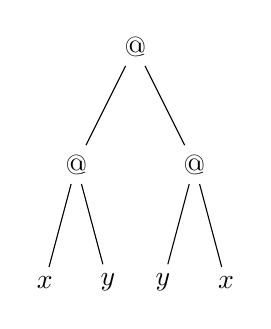
\begin{tikzpicture}
      [level 1/.style={sibling distance=15mm},
        level 2/.style={sibling distance=8mm}]
  \node at (0,0) {@}
  child { node {@}
      child {node {$x$}}
      child { node {$y$} }}
  child { node {@} 
      child {node {$y$}}
      child { node {$x$} }};
 \end{tikzpicture}

  \item

    \

    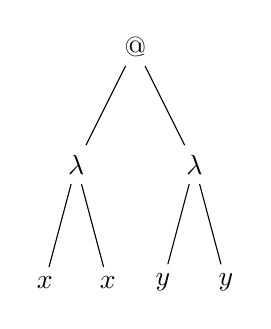
\begin{tikzpicture}
      [level 1/.style={sibling distance=15mm},
        level 2/.style={sibling distance=8mm}]
  \node at (0,0) {@}
  child { node {$\lambda$}
      child {node {$x$}}
      child { node {$x$} }}
  child { node {$\lambda$} 
      child {node {$y$}}
      child { node {$y$} }};
 \end{tikzpicture}


  \item

    \

    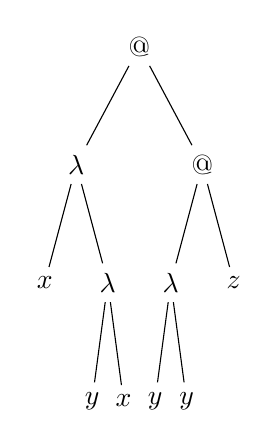
\begin{tikzpicture}
      [level 1/.style={sibling distance=16mm},
        level 2/.style={sibling distance=8mm},
          level 3/.style={sibling distance=4mm}]
  \node at (0,0) {@}
  child { node {$\lambda$}
      child {node {$x$}}
      child { node {$\lambda$}
        child {node {$y$}}
        child {node {$x$}}}}
  child { node {@}
    child { node {$\lambda$} 
        child {node {$y$}}
        child { node {$y$} }}
    child { node {$z$}}};
 \end{tikzpicture}



  \item

    \

    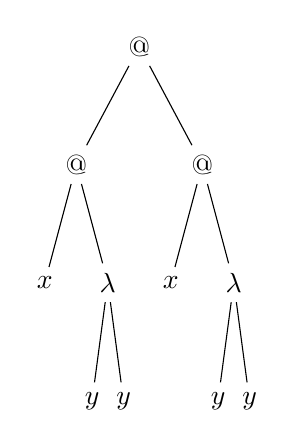
\begin{tikzpicture}
      [level 1/.style={sibling distance=16mm},
        level 2/.style={sibling distance=8mm},
          level 3/.style={sibling distance=4mm}]
  \node at (0,0) {@}
  child { node {@}
      child {node {$x$}}
      child { node {$\lambda$}
        child {node {$y$}}
        child {node {$y$}}}}
  child { node {@}
    child { node {$x$}}
    child { node {$\lambda$} 
        child {node {$y$}}
        child { node {$y$} }}};
 \end{tikzpicture}


  \end{enumerate}


  \end{enumerate}
  
\subsection{Kinds of variable occurrences}

 For each of the given terms, draw them in tree form and then
 indicate, in the same way as in Figure~\ref{fig:varocc}, which
 variable occurrences are binding (please underline), which are bound
 (please circle), and which are free (please box):
\begin{enumerate}

\item $y$

\vspace{.5cm}
\item $\lambda\, y.\ y$

\vspace{.5cm}
\item $(\lambda\, x.\, x\ x)\ y$

\vspace{.5cm}
\item $\lambda\, x.\, (\lambda\, y.\, x)\ y$

\vspace{.5cm}
\item $\lambda\, y.\, \lambda\, z.\, x\ y\ y\ (w\ z)$

\vspace{.5cm}
\end{enumerate}

\subsection{Capture-avoiding substitution}

For each of the following, write the result of the substitution or that it is undefined.

\begin{enumerate}
\item $[x/y]\lam{z}{y\ y}$
  
  \vspace{.5cm}

\item $[(x\ x)/y]\lam{z}{z\ (y\ y)}$

  \vspace{.5cm}

\item $[(x\ x)/y]\lam{y}{z\ y}$

  \vspace{.5cm}

\item $[\lam{x}{x}/y]\lam{z}{y\ \lam{y}{y\ z}}$

  \vspace{.5cm}

\item $[\lam{x}{y}/z]\lam{y}{y\ z}$
  \end{enumerate}


\subsection{Single-step $\beta$-reduction}

\begin{enumerate}
  \item Each of the following reductions is allowed by Definition~\ref{def:betactxt}.  For each reduction, indicate the instantiations of the meta-variables $x$, $t$, $t'$, and $t''$ of Definition~\ref{def:betactxt} (as in the examples in Section~\ref{sec:betaex}).
    \begin{enumerate}
    \item $\lam{x}{(\lam{y}{y})\ \lam{z}{z}}\ \betar \lam{x}{\lam{z}{z}}$
      \vspace{.5cm}
    \item $(\lam{y}{y})\ (z\ z)\ z\ \betar z\ z\ z$
      \vspace{.5cm}
    \item $z\ (\lam{y}{(\lam{z}{z\ z})\ (y\ y)}) \betar z\ \lam{y}{y\ y\ (y\ y)}$
      \vspace{.5cm}
    \item $(\lam{x}{\lam{y}{x\ x}})\ (z\ \lam{z}{z}) \betar \lam{y}{z\ (\lam{z}{z})\ (z\ \lam{z}{z})}$
      \vspace{.5cm}
    \item $(\lam{x}{\lam{y}{y}})\ z \betar \lam{y}{y}$
      \vspace{.5cm}
    \end{enumerate}

  \item Write derivations using the rules of Figure~\ref{fig:betar} for the $\beta$-reductions of parts (a), (b), (c) of the previous problem.

   \end{enumerate}

\subsection{$\alpha$-equivalence}

For each pair of terms, indicate whether or not they are $\alpha$-equivalent:
\begin{enumerate}
\item $\lam{x}{\lam{y}{y\ x}}$ and $\lam{x}{\lam{x}{y\ x}}$
  \vspace{.5cm}
\item $x\ \lam{y}{x}$ and $x\ \lam{w}{x}$
  \vspace{.5cm}
\item $x\ \lam{y}{x}$ and $y\ \lam{x}{y}$
  \vspace{.5cm}
\item $\lam{z}{(\lam{x}{x\ z})\ \lam{y}{z\ y}}$ and $\lam{q}{(\lam{y}{y\ q})\ \lam{y}{q\ y}}$
  \vspace{.5cm}
\end{enumerate}

\subsection{Multi-step $\beta$-reduction}

\begin{enumerate}

\item Write maximal $\curva$-reduction sequences starting with the given term.  Be careful with your renamings!

\begin{enumerate}
\item $\lam{y}{(\lam{x}{\lam{y}{x\ (x\ y)}})\ \lam{x}{y\ x}}$
  \vspace{.5cm}
\item $\lam{x}{\lam{y}{(\lam{z}{\lam{y}{\lam{x}{z\ z}}})\ \lam{z}{x\ y}}}$
  \vspace{.5cm}
\end{enumerate}

% answer: \delta app (in terms of Chapter 2)
\item Find an example of a term $t$ and number $n$ of $\beta$-steps where
  \begin{itemize}
  \item there exists a term $t'$ such that $t (=_\alpha\ \leadsto_\beta^n\ =_\alpha\ \leadsto_\beta) t'$, but
  \item there does not exist a term $t'$ such that $t (=_\alpha\ \leadsto_\beta^{n+1}) t'$.
  \end{itemize}
  \noindent In other words, this problem asks you to find an example of a term where a second $\alpha$-equivalence step is required in order to
  complete a sequence of $\beta$-reductions.  As a hint (because the problem is a bit tricky):
  \begin{itemize}
  \item If all bound and free variables are distinct from each other, then it is never necessary to rename to perform a single $\beta$-reduction, so it might seem like an initial $=_\alpha$-step would suffice to obviate any subsequent renamings... 
    \item ...but it is not! Ask yourself if there is a way that starting with a term where all bound and free variables are distinct from each other, one could arrive at a term that does not have that property; and then use this to construct a term where a second $=_\alpha$-step is required.

  \end{itemize}
\end{enumerate}

\chapter{Programming in Lambda Calculus}
\label{ch:prog}

\section{Basic functions}
\label{sec:basicfuncs}

Let us consider a few basic lambda terms that are useful for
programming in lambda calculus.  We will give names to the terms we
consider, as meta-linguistic abbreviations.  Let us use the syntax $N
:= t$ to indicate (in our meta-language) that we wish to use name $N$
as an abbreviation for term $t$.  In all cases, our choice of names
will be justified by the behavior of the term when applied to various
arguments.  By behavior, I mean the term's $\beta$-reductions.

\paradef{.5}{The identity function.} 
\[
\textit{id} := \lam{x}{x}
\]
\noindent This term really does behave like the mathematical
(set-theoretic, let us say) identity function, since if we apply
\textit{id} to anything, we just get back that same value.\index{identity \textit{id}}  We have

\[
\textit{id}\ t \ \ \betaa^* \ \ t
\]

\paradef{0}{Self-application operator.}
\[
\delta := \lam{x}{x\ x}
\]
\noindent This operator applies input $x$ to $x$. \index{self-application $\delta$}
We also have
\[
\Omega := \delta\ \delta
\]
\noindent This term has no normal form, reducing forever to itself:\index{diverging term $\Omega$}
\[
\begin{array}{ll}
  \underline{\delta}\ \delta & = \\
  \underline{(\lam{x}{x\ x})\ \delta} & \betaa \\
  \delta\ \delta &\
\end{array}
\]

\paradef{0}{Composition.}
\[
\textit{compose} := \lam{f}{\lam{g}{\lam{x}{f\ (g\ x)}}}
\]
\noindent This term can be applied to any terms $f$ and $g$, and it
will return a term that behaves like their composition: it applies $f$
after $g$ to its input $x$.  It is nice to borrow mathematical notation for
function composition and write $f \circ g$ for $\textit{compose}\ f\ g$.
Here are a few examples using \textit{compose}:\index{composition \textit{compose} (or $\circ$)}
\begin{itemize}
\item $\textit{id} \circ \textit{id} \ \ \betaa^*\ \ \textit{id}$
\item $\delta\circ \delta \ \ \betaa^*\ \ \lam{x}{x\ x\ (x\ x)}$:
\[
\begin{array}{ll}
  \underline{\delta\circ \delta} & = \\
  \underline{\textit{compose}}\ \delta\ \delta & = \\
  \underline{(\lam{f}{\lam{g}{\lam{x}{f\ (g\ x)}}})\ \delta}\ \delta & \betaa \\
  \underline{(\lam{g}{\lam{x}{\delta\ (g\ x)}})\ \delta} & \betaa \\
  \lam{x}{\delta\ (\delta\ x)} & \betaa \\
  \lam{x}{\delta\ \underline{(\delta\ x)}} & \betaa \\
  \lam{x}{\underline{\delta\ (x\ x)}} & \betaa \\
  \lam{x}{(x\ x)\ (x\ x)} & \ 
\end{array}
\]
  
\end{itemize}

\paradef{.5}{Application operator.}
\[
\textit{app} := \lam{x}{\lam{y}{x\ y}}
\]
\noindent This term takes in inputs $x$ and $y$ and returns the result of applying $x$ to $y$.  So it is a term which acts like the term construct of application.

\section{Representing numbers with the Church encoding}
\label{sec:churchenc}

For Church's original goal of a foundation for mathematics, it is
paramount that there is some way to represent natural numbers, and the
intuitively computable operations on them, as lambda terms.  Happily,
there are several such \emph{lambda encodings} for representing data
as lambda terms.  Here we see the first, which is Church's own encoding.\index{Church encoding}

Any lambda encoding must represent data as lambda terms implementing
some behavioral interface.  That is, data are defined by what they do,
not what they are.  The idea of the Church encoding more specifically
is to define numbers as their own iteration functions: functions which
take in another function $f$ and starting point $x$, and repeatedly
call $f$ starting with $x$.  Let us write $\rep{n}$ to mean the lambda
term representing $n\in\mathbb{N}$.  Then the Church encoding defines:

\[
\begin{array}{lll}
  \rep{n} & = & \lam{f}{\lam{x}{\underbrace{f \ (\cdots\  (f}_{n}\ x))}}
\end{array}
\]
\noindent So we have these concrete examples:

\[
\begin{array}{lll}
  0 & := & \lam{f}{\lam{x}{x}} \\
  1 & := & \lam{f}{\lam{x}{f\ x}} \\
  2 & := & \lam{f}{\lam{a}{f\ (f\ x)}} \\
  3 & := & \lam{f}{\lam{a}{f\ (f\ (f\ x))}} \\  
  \multicolumn{3}{l}{\cdots}
\end{array}
\]

\noindent In passing, we may observe that $1$ and $\textit{app}$ are $\alpha$-equivalent
terms.  When representing data as lambda terms, such coincidences
sometimes occur.

\section{Operations on Church-encoded natural numbers}

Let us see now how to define some basic operations on Church-encoded
natural numbers.

\paradef{.5}{Successor.} The mathematical successor
operation on $\mathbb{N}$ takes in $n$
and returns $n+1$ (i.e., the next number).  Here is the definition for
Church-encoded naturals:
\[
\textit{succ}\ :=\ \lam{n}{\lam{f}{\lam{x}{f\ (n\ f\ x)}}}
\]
\noindent To understand this, let us first see an example:
\[
\begin{array}{ll}
  \underline{\textit{succ}}\ 2 & = \\
  \underline{(\lam{n}{\lam{f}{\lam{x}{f\ (n\ f\ x)}}})\ 2} & \betaa \\
  \lam{f}{\lam{x}{f\ (\underline{2}\ f\ x)}} & = \\
  \lam{f}{\lam{x}{f\ (\underline{\lam{f}{(\lam{x}{f\ (f\ x)})}\ f}\ x)}} & \betaa \\
  \lam{f}{\lam{x}{f\ (\underline{(\lam{x}{f\ (f\ x)})\ x})}} & \betaa \\
  \lam{f}{\lam{x}{f\ (f\ (f\ x))}} & = \\
  3
\end{array}
\]
More generally, if $n\in\mathbb{N}$, then $\textit{succ}\ \rep{n}$ reduces to $\rep{n+1}$.

\paradef{.5}{Addition.}  To compute $\rep{m+n}$ from $\rep{m}$ and $\rep{n}$, the idea is similar to that for successor, except
that here we wish to add not just one $f$ to the left of $\underbrace{f \ \cdots\  (f }_{n}\ x)$, but $m$ applications of $f$.  For
then we would have $m+n$ applications of $f$ as desired for $\rep{m+n}$.  And fortunately, $\rep{m}$ itself gives us the power
to apply $f$ $m$ times to some starting value $Q$, by writing $m\ f\ Q$.  Here, we want $n\ f\ x$ for $Q$.  So the definition
of addition is:
\[
\textit{add} \ := \ \lam{m}{\lam{n}{\lam{f}{\lam{x}{m\ f\ (n\ f\ x)}}}}
\]

\paradef{0}{Predecessor.} Kleene was the first to crack the puzzle of how to compute the $\rep{n}$ from $\rep{n+1}$.
His definition is somewhat complicated, so here is a simpler one.  To my knowledge, this is original.  
\[
\begin{array}{lll}
\textit{just} & := & \lam{n}{\lam{j}{\lam{k}{j\ n}}} \\
\textit{pred} & := & \lam{n}{n\ (\lam{m}{\textit{just}\ (m\ \textit{succ}\ 0)})\ 0\ \textit{id}\ 0}
\end{array}
\]
\noindent Writing $F$ for $\lam{m}{\textit{just}\ (m\ \textit{succ}\ 0)}$, let us first see how $2\ F\ 0$ computes:
\[
\begin{array}{ll}
  \underline{2\ F}\ 0 & \betaa \\
  \underline{(\lam{a}{F\ (F\ a)})\ 0} & \betaa \\
  F\ (\underline{F\ 0}) & \betaa \\
  F\ (\textit{just}\ (\underline{0\ \textit{succ}}\ 0)) & \betaa \\
  F\ (\textit{just}\ (\underline{\lam{a}{a}\ 0})) & \betaa \\
  F\ (\underline{\textit{just}\ 0}) & \betaa \\
  \underline{F\ \lam{j}{\lam{k}{j\ 0}}} & \betaa \\    
  \textit{just}\ (\underline{(\lam{j}{\lam{k}{j\ 0}})\ \textit{succ}}\ 0) & \betaa \\
  \textit{just}\ (\underline{(\lam{k}{\textit{succ}\ 0})\ 0}) & \betaa \\
  \underline{\textit{just}\ (\textit{succ}\ 0)} & \betaa \\
  \lam{j}{\lam{k}{j\ (\textit{succ}\ 0)}} & \ 
\end{array}
\]
\noindent Now here is the reduction for $\textit{pred}\ 2$:
\[
\begin{array}{ll}
  \underline{\textit{pred}\ 2} & \betaa \\
  \underline{2\ F\ 0}\ \textit{id}\ 0 & \betaa^* \textnormal{[by above reduction sequence]}\\
  \underline{(\lam{j}{\lam{k}{j\ (\textit{succ}\ 0)}})\ \textit{id}}\ 0 & \betaa \\
  \underline{(\lam{k}{\textit{id}\ (\textit{succ}\ 0)})\ 0} & \betaa \\
  \underline{\textit{id}\ (\textit{succ}\ 0)} & \betaa \\
  \underline{\textit{succ}\ 0} & \betaa^* \\
  1 &\ 
\end{array}
\]
  

\paradef{0}{Another predecessor.}  Here is a different, trickier definition of predecessor, which one can find online (sadly, I do
not know who invented it):
\[
\textit{pred}\ :=\ \lam{n}{\lam{f}{\lam{x}{n\ (\lam{g}{\lam{h}{h\ (g\ f)}})\ (\lam{h}{x})\ \textit{id}}}}
\]
\noindent To understand how this works, let us write $F$ for $\lam{g}{\lam{h}{h\ (g\ f)}}$, and $A$ for $\lam{h}{x}$, and
see how $3\ F\ A$ computes:
\[
\begin{array}{ll}
  \underline{3\ F}\ A & \betaa \\
  (\lam{x}{F\ (F\ (F\ x))})\ A & \betaa \\
  F\ (F\ (\underline{F\ A})) & = \\
  F\ (F\ (\underline{(\lam{g}{\lam{h}{h\ (g\ f)}})\ \lam{h}{x}})) & \betaa \\  
  F\ (F\ (\lam{h}{h\ \underline{((\lam{h}{x})\ f)}})) & \betaa \\
  F\ (\underline{F}\ (\lam{h}{h\ x})) & = \\
  F\ (\underline{(\lam{g}{\lam{h}{h\ (g\ f)}})\ (\lam{h}{h\ x})}) & \betaa \\      
  F\ (\lam{h}{h\ \underline{((\lam{h}{h\ x})\ f)}}) & \betaa \\
  \underline{F}\ (\lam{h}{h\ (f\ x)}) & = \\
  \underline{(\lam{g}{\lam{h}{h\ (g\ f)}})\ (\lam{h}{h\ (f\ x)})} & \betaa \\
  \lam{h}{h\ \underline{((\lam{h}{h\ (f\ x)})\ f)}} & \betaa \\
  \lam{h}{h\ (f\ (f\ x))} & \
\end{array}
\]

What is happening here?  We see that $3\ F\ A$ has reduced to something similar to $f\ (f\ (f\ x))$, but
with a critical twist: we have $\lambda$-abstracted away the function for the first call to $f$, leaving
the other calls intact.  This gives us what we could think of as a ``flexible'' version of $f\ (f\ (f\ x))$, where we get
to choose which function to call instead of $f$ for the outer application.  And the definition of predecessor makes use of this flexibility
by applying the whole result to \textit{id}.  That produces, then, just $f\ (f\ x)$.  So, understanding $F$ and $A$ to be grafted
into the expression on the second line below (capturing their free variables $f$ and $x$), we have
\[
\begin{array}{ll}
  \textit{pred}\ 3 & \betaa^* \\
  \lam{f}{\lam{x}{\underline{3\ F\ A}\ \textit{id}}} & \betaa^* \\
  \lam{f}{\lam{x}{\underline{(\lam{h}{h\ (f\ (f\ x))})\ \textit{id}}}} & \betaa \\
  \lam{f}{\lam{x}{\underline{(\textit{id}\ (f\ (f\ x)))}}} & \betaa \\
  \lam{f}{\lam{x}{f\ (f\ x)}} & = \\  
  2 &\ 
\end{array}
\]

In some ways this is similar, as perhaps is inevitable, to the first
version of predecessor we saw: a value is computed from $\rep{n}$ that
is like $\rep{n}$ but allows calling another function -- in particular, \textit{id} -- instead of a
final successor.  In this second version of predecessor, that
value is computed underneath bindings of $f$ and $x$, so that
\textit{id} gets called on applications of $f$ to $x$.  In the
first version of predecessor, \textit{id} gets called on the entire
predecessor term, including bindings of $f$ and $x$.

\section{Representing booleans}
\label{sec:bool}

A simpler datatype than that of the natural numbers is the boolean
type, with values \textit{true} and \textit{false}.  The Church
encoding of this type is
\[
\begin{array}{lll}
  \textit{true} & := & \lam{x}{\lam{y}{x}} \\
  \textit{false} & := & \lam{x}{\lam{y}{y}}
\end{array}
\]
\noindent Each boolean accepts two inputs (one at a time), and returns
one of these.  \textit{true} returns the first, while \textit{false}
returns the second.  Based on this idea, it is easy to see how to define
various boolean operations:
\[
\begin{array}{lll}
  \textit{not} & := & \lam{x}{x\ \textit{false}\ \textit{true}} \\
  \textit{and} & := & \lam{x}{\lam{y}{x\ y\ \textit{false}}}
\end{array}
\]
\noindent We negate (with \textit{not}) a boolean by applying it to
\textit{false} and then \textit{true}.  If the boolean itself is
\textit{true}, then it will return the first of these two inputs,
namely \textit{false}; if it is \textit{false}, it will return
\textit{true}.  This is the desired behavior.  Similarly, \textit{and}
takes in inputs \textit{x} and \textit{y}.  It returns the result of
applying \textit{x} to \textit{y} and then \textit{false}.  If
\textit{x} is \textit{true}, then the result will be \textit{y}; and
this is what we would like for conjunction, since if the first boolean
(\textit{x}) is true, the conjunction's value coincides with the value
of the second (\textit{y}): true if \textit{y} is true, and false if
\textit{y} is false.  And if \textit{x} is \textit{false}, then the
second input (out of \textit{y} and \textit{false}) will be chosen; again,
the desired behavior, since this means conjoining \textit{false} with
anything will reduce to \textit{false}.

It is worth emphasizing that applying boolean operations to values
that are not booleans does not result in an error as it might
in some programming languages.  Here, every lambda term has a well-defined
behavior in the form of its $\beta$-reductions.  But the results of
applications violating the intuitive typings we have in mind for
these operations may be somewhat inscrutable.

\section{Ordered pairs}

It is often convenient to program with a representation of ordered pairs $(x,y)$, given representations of $x$ and $y$.
To construct the representation of a pair, we use this function:
\[
\textit{pair} \ :=\ \lam{x}{\lam{y}{\lam{c}{c\ x\ y}}}
\]
\noindent The idea is that given the components $x$ and $y$ of the
pair, we represent (by the \textit{pair} function) the pair itself as
$\lam{c}{c\ x\ y}$.  This definition embodies the idea that a pair of
$x$ and $y$ is something that can make $x$ and $y$ available for
subsequent computation.  This is done in the encoding by applying the
pair to a function which is expecting the components.

For example, we may define \textit{fst} (``first'') and \textit{snd}
(``second''; these names are often used for these operations in
functional programming languages) as follows:
\[
\begin{array}{lll}
  \textit{fst} & := & \lam{p}{p\ \textit{true}} \\
  \textit{snd} & := & \lam{p}{p\ \textit{false}}
\end{array}
\]
\noindent Since \textit{true} returns the first of two arguments, and
\textit{false} the second, they are used to select either the first or
the second component, respectively, when passed as an argument to the
pair.  (As usual, these functions assume input \textit{p} is a pair
of the form $\lam{c}{c\ x\ y}$, and may give unexpected results
if applied to terms not of that form.)

\section{Representing numbers with the Scott encoding}

In Section~\ref{sec:churchenc}, we saw an elegant representation of
numbers as lambda terms, called the Church encoding.  Every number $n$
is represented as the $n$-fold composition operator.  While many
functions are concisely definable this way, the predecessor operation
required quite some ingenuity, and is asymptotically less efficient
than we might reasonably expect (taking time linear in $n$, instead of
constant time).  In this section, we consider an alternative lambda
encoding due to Dana Scott, which has a straightforward constant-time
predecessor.  With the Scott encoding, each number can be thought of
as a function $t$ that informs the caller whether $t$ represents a
successor number or zero.  In the former case, it also provides the
caller with the representation of the predecessor. The definition is:
\[
\begin{array}{lll}
  0 & := & \lam{f}{\lam{x}{x}} \\
  1 & := & \lam{f}{\lam{x}{f\ 0}} \\
  2 & := & \lam{f}{\lam{x}{f\ 1}} \\
  \multicolumn{3}{l}{\cdots} \\
  \rep{n+1} & := & \lam{f}{\lam{x}{f\ \rep{n}}} \\
  \multicolumn{3}{l}{\cdots} 
\end{array}
\]
So every $\rep{n}$ accepts two inputs $f$ and $x$, and if
$n$ is $0$, returns $x$; and if $n$ is $m+1$ for some $m$, returns
$f\ \rep{m}$.  This makes available the predecessor $\rep{m}$, and
thus the actual predecessor function is easily defined:
\[
\textit{pred} \ := \ \lam{n}{n\ \textit{id}\ 0}
\]
\noindent Here, \textit{id} is passed for $f$ and $0$ for $x$.  This means
that for any Scott-encoded successor number, we have the following reduction:
\[
\begin{array}{ll}
  \underline{\textit{pred}}\ \rep{n+1} & = \\
\underline{(\lam{n}{n\ \textit{id}\ 0})\ \rep{n+1}} & \betaa \\
\underline{\rep{n+1}}\ \textit{id}\ 0 & = \\
\underline{(\lam{f}{\lam{x}{f\ \rep{n}}})\ \textit{id}}\ 0 & \betaa \\
\underline{(\lam{x}{\textit{id}\ \rep{n}})\ 0} & \betaa \\
\underline{\textit{id}\ \rep{n}} & \betaa \\
\rep{n} & \
\end{array}
\]
\noindent And this is the desired result: $\textit{pred}\ \rep{n+1}
\betaa^* \rep{n}$.  Furthermore, we can see that this reduction required
four steps of $\beta$-reduction, independent of the value of $n$.
This is in contrast to the case with the Church encoding, where the
number of steps was proportional to $n$.

It is obvious from the encoding that the successor function \textit{succ} for Scott-encoded numbers should be:
\[
\textit{succ}\ := \ \lam{n}{\lam{f}{\lam{x}{f n}}}
\]

\section{The Y combinator}
\label{sec:y}

While it is very straightforward to define predecessor on
Scott-encoded numbers, other operations pose a problem.  The Church
encoding takes $n$-fold iteration as the representation of $n$, and
hence has no difficulty defining iterative functions.  Not so the
Scott encoding, and indeed, the only natural way to recurse is to
avail ourselves of a term implementing \emph{general recursion} (this
is recursion that may fail to terminate).  (It should be noted that
there is an extremely tricky way to derive iteration for Scott encodings, but
we will not consider this here~\cite{lepigre+19}.)

General recursion in lambda calculus is provided using a term traditionally
denoted $Y$:
\[
Y \ :=\ \lam{f}{(\lam{x}{f\ (x\ x)})\ (\lam{x}{f\ (x\ x)})}
\]
\noindent This term is usually called a \emph{combinator}, which is an
informal notion indicating that a lambda term is of interest primarily
for use as a building block for defining other functions (as opposed,
say, to implementing some particular algorithm valuable in its own
right).\index{combinator}\index{Y combinator} In this sense, some other terms we have
encountered so far, like identity and composition functions
(\textit{compose}, \textit{id} of Section~\ref{sec:basicfuncs}), are
also reasonably considered combinators.

Terminology aside, let us see how the $Y$ combinator works and how we
can use it to define operations on Scott-encoded numbers.  Suppose $t$ is any
lambda term not containing $x$ free.  Then we have:
\[
\begin{array}{ll}
  \underline{Y}\ t & = \\
  \underline{(\lam{f}{(\lam{x}{f\ (x\ x)})\ (\lam{x}{f\ (x\ x)})})\ t} & \betaa \\
  \underline{(\lam{x}{t\ (x\ x)})\ (\lam{x}{t\ (x\ x)})} & \betaa \\
  t\ \underline{((\lam{x}{t\ (x\ x)})\ (\lam{x}{t\ (x\ x)}))} & =_\beta \\
  t\ (Y\ t)
\end{array}
\]
\noindent So we see that $Y\ t$ is $\beta$-equivalent to $t\ (Y\ t)$.  This fact is so important that
it is worth highlighting as an equation:
\[
Y\ t\ =_\beta \ t\ (Y\ t)
\]
\noindent Swapping sides will shortly be revealing:
\[
t\ (Y\ t)\ =_\beta \ Y\ t
\]
\noindent This matches the form of a fixed-point equation for $t$.  In mathematics, a fixed point of a function $F$ is an input $X$ such that
\[
F(X) = X
\]
\noindent Here, with application of lambda terms playing the role of function invocation, and $\beta$-equivalence taking the place of equality,
we can write this as:
\[
F\ X =_\beta X
\]
\noindent For term $t$, this becomes
\[
t\ X =_\beta X
\]
\noindent And indeed, the equation we derived above is of this form, with $Y\ t$ for $X$.

Now what is the significance of this?  It shows us that, contrary to
what we usually find in mathematics, in lambda calculus every function
has a fixed point.  How peculiar!  Certainly some mathematical
functions have fixed points.  Take (mathematical) predecessor on
natural numbers, with the assumption that \textit{pred} of $0$ is $0$.
Then $0$ is a fixed point of \textit{pred}.  But consider boolean negation.
There is no boolean $b$ such that $\textit{not}\ b$ equals $b$ (neither possible
value for $b$, namely \textit{true} or \textit{false}, works).  Strangely, though,
in lambda calculus, we have just seen the general equation of $t\ (Y\ t)$ and $Y\ t$.
This means that
\[
\textit{not}\ (Y\ \textit{not}) =_\beta Y\ \textit{not}
\]
\noindent Something unusual is going on, and indeed, as we will see when we
turn to denotational semantics of lambda calculus, interpreting lambda calculus
in set theory requires significant ingenuity.

But to remain at the linguistic level for the moment, let us try to get an intuition
for how every term $t$ can have $Y\ t$ for a fixed point.  Let us write $U$ for $\lam{x}{t\ (x\ x)}$.  We have seen that
\[
\begin{array}{ll}
  \underline{Y\ t} & \betaa \\
  \underline{U\ U} & \betaa \\
  t\ (U\ U)&\ 
\end{array}
  \]
\noindent  This reduction sequence may then be continued as long as we wish:
\[
\begin{array}{ll}
  t\ \underline{(U\ U)}&\betaa \\
  t\ (t\ \underline{(U\ U)})&\betaa \\  
  t\ (t\ (t\ \underline{(U\ U)}))&\betaa \\
  \multicolumn{2}{l}{\cdots}
\end{array}
\]
\noindent If we had some notion of infinite lambda term, we might identify the limit of this infinite reduction sequence,
as this infinite right-nested application of $t$:
\[
t\ (t\ (t\ \cdots
\]
\noindent One can indeed develop an infinitary lambda calculus
allowing infinitary terms like this~\cite{kennaway1997}; but this is
beyond the scope of the book.  But with an infinitary term like
this as an informal guiding intuition, we can see how the fixed-point equation
makes sense.  $Y\ t$ denotes (informally) an infinite
right-nested application of $t$.  Applying $t$ one more time to this
does not change the infinite application, as it is still infinite!

Note that $U\ U$ is a lot like $\delta\ \delta$:
\[
\begin{array}{lll}
  U\ U & = & (\lam{x}{t\ (x\ x)})\ \lam{x}{t\ (x\ x)} \\
  \delta\ \delta & = & (\lam{x}{x\ x})\ \lam{x}{x\ x}
\end{array}
\]
\noindent We have just inserted $t$, but otherwise retain the central idea of self-application
for divergence.

How is this esoterically explained construction useful for programming?  Contrast
the situation with iteration using Church-encoded numbers.  There, $\rep{n}$ gives us the
power to repeat a function $n$ times:
\[
\underbrace{t\ \cdots\ (t}_n\ x)
\]
\noindent But what if we need to repeat a function more times than
just $n$ times?  We could imagine somehow increasing how many times
the composition is iterated, to some bigger number $n'$.  But the most
computationally powerful option is to extend the $n$-fold iteration of
$t$ to an infinite iteration of $t$:
\[
t\ (t\ (t\ \cdots
\]
\noindent But this is just what (informally) $Y\ t$ gives us!  So we
are using the power of diverging computation which we get through
self-application, to allow ourselves as many iterations of $t$ as we
could possibly need.  Fundamental results of recursion theory then
imply that we will of necessity need to accept the possibility of
divergence: we have given ourselves the ability to apply $t$ as many
times as we wish, and we cannot rule out the possibility that it gets
applied infinitely many times with no normal form reachable.

But there is still a puzzle.  How can we ever reach any normal form when
$Y\ t$ has an infinite reduction sequence?  The answer is that existence
of a single infinite reduction sequence does not mean all reduction
sequences are infinite.  Indeed, for a very simple example, consider
\[
(\lam{x}{\lam{y}{y}})\ \Omega
\]
\noindent This term has both an infinite reduction sequence, and also infinitely many finite reduction sequences.  For examples of the first and second, in order, consider:
\[
\begin{array}{l}
  (\lam{x}{\lam{y}{y}})\ \underline{\Omega}\ \betaa\ (\lam{x}{\lam{y}{y}})\ \underline{\Omega}\ \betaa \ \cdots \\
  \underline{(\lam{x}{\lam{y}{y}})\ \Omega} \ \betaa \ \lam{y}{y}
\end{array}
\]
\noindent The normalizing reduction sequence (the second one) drops out the non-normalizing $\Omega$ subterm.
Similarly, in our infinitary term
\[
t\ (t\ (t\ \cdots
\]
\noindent it could happen that there is a reduction to a normal form where an application of $t$ ends up dropping
its argument.  We will see an example next.

\section{Recursive operations on Scott-encoded numbers}

Let us define addition on Scott-encoded numbers using the $Y$ combinator.  The idea is that we wish to implement the following
system of recursive equations, using $Y$ to implement the recursion:
\[
\begin{array}{lll}
  \textit{add}\ 0\ m & = & m \\
  \textit{add}\ (\textit{succ}\ p)\ m & = & \textit{succ}\ (\fbox{\textit{add}}\ p\ m)
\end{array}
\]
\noindent Since the Scott-encoding gives us a way to distinguish whether a number is $0$ or a successor number, we can
easily choose whether between these equations based on the first input.  We then need to use $Y$ to implement the framed
recursion on the right-hand side of the second equation.  The definition is, the following, using helper definition \textit{addh} for
easier consideration below:
\[
\begin{array}{lll}
  \textit{addh} & := & \lam{\textit{add}}{\lam{n}{\lam{m}{n\ (\lam{p}{\textit{succ}\ (\textit{add}\ p\ m)})\ m}}} \\
  \textit{add} & := & Y\ \textit{addh}
  \end{array}
\]
\noindent Let us see how this works with an example, writing $U$ for $\lam{x}{\textit{addh}\ (x\ x)}$:
\[
\begin{array}{ll}
  \underline{\textit{add}}\ 2\ 2 & = \\
  \underline{Y\ \textit{addh}}\ 2\ 2 & \betaa \\
  \underline{U\ U}\ 2\ 2 & \betaa \\  
  \underline{\textit{addh}}\ (U\ U)\ 2\ 2 & = \\
  \underline{(\lam{\textit{add}}{\lam{n}{\lam{m}{n\ (\lam{p}{\textit{succ}\ (\textit{add}\ p\ m)})\ m}}})\ (U\ U)}\ 2\ 2 & \betaa \\  
  \underline{(\lam{n}{\lam{m}{n\ (\lam{p}{\textit{succ}\ (U\ U\ p\ m)})\ m}})\ 2\ 2} & \betaa^2 \\
  \underline{2}\ (\lam{p}{\textit{succ}\ (U\ U\ p\ 2)})\ 2 & = \\
  \underline{(\lam{f}{\lam{x}{f\ 1}})\ (\lam{p}{\textit{succ}\ (U\ U\ p\ 2)})\ 2} & \betaa^2 \\
  \underline{(\lam{p}{\textit{succ}\ (U\ U\ p\ 2)})\ 1} & \betaa \\
  \textit{succ}\ \underline{(U\ U\ 1\ 2)}) & \betaa^* \\
  \textit{succ}\ (\textit{succ}\ \underline{(U\ U\ 0\ 2)}) & \betaa^* \\
  \textit{succ}\ (\textit{succ}\ 2) & \betaa^* \\
  4 &\ 
  \end{array}
\]
\noindent We see in detail that $U\ U\ \rep{n+1}\ m$ reduces to
$\textit{succ}\ (U\ U\ \rep{n}\ m)$.  So we peel successors off the
first argument until we reach $0$, and then we return the second
argument (i.e., $m$).

\section{A direct approach to recursion on Scott-encoded numbers}

Instead of using the $Y$ combinator, it is possible to recurse
directly on Scott-encoded numbers.  A Scott-encoded number takes in a
function $f$ to call with the predecessor if the number is non-zero,
and a value $x$ to return if the number is zero.  The key idea,
attributed by Lepigre and Rafalli to Michel Parigot, is to have $f$
and $x$ themselves expect to be called with $f$ and $x$
again~\cite{lepigre:rafalli19}.  This enables in particular $f$ to
recurse.

Here is a definition of addition for the Scott encoding,
using this idea. I have abstracted out $f$ and $x$ for this
case, to help make clear where there is a self-application
happening.  The base case $x$ depends, in the definition of addition,
on the second addend, so we need to write $x\ m$ in the definition
of \textit{add}, instead of just $x$.
\begin{eqnarray*}
f & := & \lam{p}{\lam{s}{\lam{z}{\textit{succ}\ (p\ s\ z\ s\ z)}}} \\
x & := & \ \lam{m}{\lam{s}{\lam{z}{m}}} \\
\textit{add} & := & \lam{n}{\lam{m}{n\ f\ (x\ m)\ f\ (x\ m)}}
\end{eqnarray*}

\noindent Let us see this definition in action:

\[
\begin{array}{ll}
  \underline{\textit{add}\ 2\ 2} & \betaa^2 \\
  \underline{2\ f}\ (x\ 2)\ f\ (x\ 2) & \betaa \\
  \underline{f\ 1\ f\ (x\ 2)} & \betaa^3 \\
  \textit{succ}\ \underline{(1\ f\ (x\ 2)\ f\ (x\ 2))} & \betaa^4 \\
  \textit{succ}\ (\textit{succ}\ \underline{(0\ f\ (x\ 2)\ f\ (x\ 2))}) & \betaa \\
  \textit{succ}\ (\textit{succ}\ \underline{((x\ 2)\ f\ (x\ 2))}) & \betaa^3 \\
  \underline{\textit{succ}\ (\textit{succ}\ 2)} & \betaa^* \\    
  4
\end{array}
  \]

\section{The Parigot encoding}

Before (it seems) his discovery of a way to recurse on Scott-encoded
numbers, Parigot proposed an encoding that combines the Church and
Scott encodings:

\[
\begin{array}{lll}
  0 & := & \lam{f}{\lam{x}{x}} \\
  1 & := & \lam{f}{\lam{x}{f\ 0\ x}} \\
  2 & := & \lam{f}{\lam{x}{f\ 1\ (f\ 0\ x)}} \\
  3 & := & \lam{f}{\lam{x}{f\ 2\ (f\ 1\ (f\ 0\ x))}} \\
  \multicolumn{3}{l}{\cdots} \\
  \rep{n+2} & := & \lam{f}{\lam{x}{f\ \rep{n+1}\ (f\ \rep{n}\ (\cdots\ (f\ 0\ x)))}} \\
  \multicolumn{3}{l}{\cdots} 
\end{array}
\]

\noindent Another way to see the encoding is to observe that for every $n$,
\[
\rep{n+1}\ \betaeq\ \lam{f}{\lam{x}{f\ \rep{n}\ (\rep{n}\ f\ x)}}
\]
\noindent where $\betaeq$ denotes $\beta$-equivalence (Definition~\ref{def:betaeq})

\section{Exercises}

\subsection{$\beta$-reductions for some simple terms}

\begin{enumerate}
\item For each of the following terms, write down a $\beta$-normal form to which the term reduces.  You do not need to write out all the steps in a $\beta$-reduction sequence.  Please just give a $\beta$-normal form.

  \begin{enumerate}
  \item $\textit{app}\ \circ\ \textit{id}$
\vspace{.5cm}
  \item $\textit{app}\ \circ\ \textit{app}$
\vspace{.5cm}
  \item $\lam{z}{2\ z}$
\vspace{.5cm}
  \item $\delta\ \textit{app}$
\vspace{.5cm}
  \item $2\ 2$
\vspace{.5cm}
  \item $\textit{not}\ 2$ (as noted above, terms like this which violate intuitive typings do have a
    well-defined behavior)
\vspace{.5cm}
  \item $\textit{and}\ 1$
  \end{enumerate}

\item Please write out a maximal $\beta$-reduction sequence (renaming is not necessary, so we can use just $\betar$
  instead of $\betaa$) starting with $\textit{pred}\ 2$.

\end{enumerate}

\subsection{Programming in lambda calculus}

\begin{enumerate}
\item Define a disjunction operator (i.e., boolean ``or'') on Church-encoded booleans, and demonstrate that it is working by writing a maximal $\betaa$-reduction sequence starting with $\textit{or}\ \textit{false}\ \textit{true}$.

\item \ \textbf{[Challenge]} Find an alternative definition of \textit{pred} with similar form as above, namely
  \[
  \lam{n}{\lam{f}{\lam{x}{n\ F'\ A'\ t_1 \cdots t_k}}}
  \]
  \noindent for some terms $F'$ and $A'$ grafted into this expression (which hence might have free occurrences of $f$ or $x$ that get bound by the $\lambda$-abstractions of those two variables), and some extra terms $t_1, \cdots, t_k$.
  The critical requirement is that where $\rep{n+1}\ F\ A$ reduces (with the definition of $F$ and $A$ in the text) to $\lam{h}{h\ (\underbrace{f \cdots (f}_n\ x))}$, your version with your $F'$ and $A'$ and some of your extra terms should
  reduce to $\lam{h}{\underbrace{f \cdots (f}_n\ (h\ x))}$.

\item Define a function \textit{flip} which reverses the order of components in a pair.

\item Define a subtraction operation on Scott-encoded numbers.  Your term is free to invoke \textit{pred} for predecessor,
  and the $Y$ combinator (and other terms we have defined so far, if you wish).

  \item The term $Y\ Y$ has many different (infinite) reductions.  Try
    to indicate a little of the complexity of this term by showing
    prefixes of some of its reduction sequences.  It would be
    interesting to organize these initial parts of reduction sequences
    into a tree, so we can see how reduction can branch out in different
    ways from the starting point of $Y\ Y$.  (This problem is not concerned
    with giving an exact correct answer, but rather with showing that you
    have explored the reduction behavior of this rather exotic term.)
\end{enumerate}

\chapter{Confluence}

In this chapter, we prove a basic property of the lambda calculus,
called confluence.\index{confluence} Given a binary relation $\to$ on
a set $A$, an element $a \in A$ is confluent iff no matter which pair
of $\to$-paths we follow from $a$, ending in some elements $b$ and
$c$, there is a pair of $\to$-paths from $b$ and $c$ ending in a
common element $d$.  This can be expressed pictorially as:

\begin{center}
\begin{tikzpicture}
  \node at (0,2) (a){a};
  \node at (-2,0) (b){b};
  \node at (2,0) (c){c};
  \node at (0,-2) (d){d};

  \node at (.4,-1.85) {$*$};
  \node at (-.4,-1.85) {$*$};
  \node at (-1.85,.4) {$*$};
  \node at (1.85,.4) {$*$};

  \draw[->] (a) -- (b);
  \draw[->] (a) -- (c);
  \draw[->,dashed] (b) -- (d);
  \draw[->,dashed] (c) -- (d);  
\end{tikzpicture}
\end{center}

Confluence can be seen as a generalization of determinism
(Definition~\ref{def:det}, the property that whenever $a \to b$ and $a
\to c$, we have $b = c$).  For it might happen that we have paths from
$a$ that can reach distinct elements $b$ and $c$ (that is, $a \to^* b$
and $a \to^* c$, with $b \neq c$), but these elements can be joined
back at some element $d$ (so $b \to^*d$ and $c\to^*d$).  So $a$ is
nondeterministic, yet in a somewhat controlled way: no matter
which two paths we follow from $a$, there is always some way to
reconverge.

In this chapter, we will prove that the relation $\curva_\alpha \cup
\curva_\beta$ is confluent.  This relation subsumes the relation
$\betaa$ of single-step $\beta$-reduction with renaming
(Definition~\ref{def:betaa}), because it allows any sequence of
$\curva_\alpha$ and $\curva_\beta$ steps, while a non-trivial
$\betaa$-reduction sequence must end with a $\curva_\beta$ step.
Working with the more permissive relation will enable a cleaner
formulation of confluence.  The proof we will follow is attributed to
William Tait and Per Martin-L\"of (but never published by either of
them).  Some of our discussion is quite generic, however, and applies
to any binary relation $\to$ over some set of elements (not
necessarily terms).

We will use the notation $\abeta$ for the relation that we
will study in this chapter:

\begin{definition}
  \label{def:abeta}
  $\abeta$ is defined to be $\curva_\alpha \cup \curva_\beta$.
  \end{definition}

\section{The diamond property}

A property quite similar to confluence of a relation $\to$ is
the following:
\begin{definition}[Diamond property]
  An element $x$ has the diamond property with respect to relation
  $\to$ on set $A$ iff $x \to y$ and $x \to z$ imply that there exists an element $q$
  with $y \to q$ and $z \to q$. The relation $\to$ itself has the diamond
  property, denoted $\textit{Diamond}(\to)$, iff every element of $A$ has
  the diamond property with respect to $\to$.  \index{diamond property}
  \end{definition}
\noindent Pictorially, this is very similar to the diagram for confluence,
but without the stars:

\begin{center}
\begin{tikzpicture}
  \node at (0,1.75) (a){a};
  \node at (-1.75,0) (b){b};
  \node at (1.75,0) (c){c};
  \node at (0,-1.75) (d){d};


  \draw[->] (a) -- (b);
  \draw[->] (a) -- (c);
  \draw[->,dashed] (b) -- (d);
  \draw[->,dashed] (c) -- (d);  
\end{tikzpicture}
\end{center}

Indeed, an alternative definition of confluence of $\to$ is simply to say that $\to^*$ has the diamond property.
In this form, the following lemma states that reflexive-transitive closure preserves the diamond property:
\begin{theorem}[Star preserves diamond]
\label{thm:stardia}
  $\textit{Diamond}(\to)$ implies $\textit{Diamond}(\to^*)$
\end{theorem}
\begin{proof}
  Assume $\textit{Diamond}(\to)$ and $x$, $y$, $z$ with $x \to^*y$ and $x \to^* z$.  We proceed
  by induction on the derivation of $x \to^* y$ (recall the three rules defining the reflexive-transitive
  closure, in Figure~\ref{fig:rtcl}):

  \case{ }
  \[
  \infer{x \to^* y}{x \to y}
  \]
  \noindent Here we will proceed by an inner induction on the derivation of $x \to^* z$ to show that there
  is a $q$ with $y\to^*q$ and $z \to q$, for all $x$, $y$, and $z$ with $x\to y$.

  \case{ (inner)}
  \[
  \infer{x \to^* z}{x \to z}
  \]
  \noindent We have exactly the assumptions of the diamond property, so we can conclude that there is a $q$
  with $y \to q$ and $z \to q$.  Our inner induction requires us to show $y \to^* q$, which follows from
  this same inclusion rule whose inferences we are presently considering.

  \case{ (inner)}
  \[
  \infer{x \to^* x}{\ }
  \]
  \noindent We have learned in this case that $x = z$, since that is the only way the reflexivity
  rule could be applied to prove $x \to^*z$.  
  For whatever $q$ we select, we must prove $y \to^*q$ and $z \to q$.  
  Since $x = z$, it suffices to show $y \to^*q$ and $x \to q$.  Let us take $q$ to be $y$.
  So we must show $y \to^* y$, which follows by the reflexivity rule; and $x \to y$, which
  follows by assumption in this inner induction.

  \case{ (inner)}
  \[
  \infer{x \to^* z}{x \to^*w & w \to^* z}
  \]
  \noindent We may apply the induction hypothesis to the first premise of this
  inference.  So the $x$, $y$, and $z$ of the induction hypothesis are instantiated
  with $x$, $y$, and $w$, respectively.  The induction hypothesis then tells us that
  there is an element $q$ such that $y \to^*q$ and $w \to q$.  We may now apply the
  induction hypothesis to the second premise, where we
  instantiate $x$, $y$, and $z$ with $w$, $q$, and $z$, respectively.  This tells
  us that there is a $q'$ with $q\to^*q'$ and $z \to q'$.  Combining a couple of
  the facts we have so far (namely, $y\to^* q$ and $q\to^* q'$) using the
  transitivity rule gives us $y \to^* q'$.  And we have $z \to q'$.
  So we may take the element $q$ which we are supposed to identify, to be this $q'$.
  This concludes the inner induction.  Note that this induction could be (and often is)
  broken out as a separate lemma, since it does not need to invoke the outer induction
  hypothesis.
  
  We may now return to our outer induction:

  \case{ }
  \[
  \infer{x \to^* x}{\ }
  \]
  \noindent In this case, we have learned that $x = y$, since that is the only way a reflexivity
  inference could prove $x \to^* y$.  Our goal is to identify an element $q$ with $y \to^* q$ and $z \to^* q$,
  but since $x = y$, it suffices to find a $q$ with $x \to^* q$ and $z \to^* q$.  Take $q$ to be $z$, and
  we have $x \to^* z$ by assumption of this induction, and $z \to^* z$ by reflexivity.

  \case{ }
  \[
  \infer{x \to^* y}{x \to^* w & w \to^* y}
  \]
  \noindent By the induction hypothesis applied to the first premise, there is a $q$ with
  $w \to^* q$ and $z \to^* q$.  We may now apply the induction hypothesis to the second
  premise, instantiating $x$, $y$, and $z$ with $w$, $y$, and $q$, respectively.  This
  produces a $q'$ with $y\to^* q'$ and $q\to^* q'$.  Let us take $q'$ to be the $q$ required
  by the theorem.  Since $z\to^*q$ and $q\to^* q'$, we have $z \to^* q'$ by transitivity;
  and $y\to^* q'$ was already concluded.
  

  \end{proof}

Thanks to Theorem~\ref{thm:stardia}, we know that if we would like to establish confluence of $\abeta$, it
would suffice to prove that this relation has the diamond property.  But this is easily seen
not to be the case.  Consider the diagram in Figure~\ref{fig:betanodia}.  The term at the peak (top) of the diagram
has two redexes, shown underlined.  Down the left side of the peak we reduce the leftmost redex, and down the right
side, the rightmost.  We can indeed join the resulting terms, at term $z\ z$, but this requires two steps along the
left side of the valley (running diagonally right to $z\ z$), while needing just one step along the right
side of the valley.  This example shows:

\begin{theorem}
  $\abeta$ lacks the diamond property
\end{theorem}

It is the beautiful observation at the heart of the Tait--Martin-L\"of proof of confluence that
while $\beta$-reduction lacks the diamond property, still another relation $\Pred^\alpha$ can be defined which
satisfies the diamond property, and where $(\Pred^\alpha)^* = \betaa^*$.  This will lead us to our goal,
thanks to the following theorem:
\begin{theorem}
  \label{thm:tml}
  Let $S$ be a relation on a set $A$, and suppose that there is a relation $R$ on $A$ such that
  $\textit{Diamond}(R)$ and $R^* = S^*$.  Then $S$ is confluent.
\end{theorem}

\begin{proof}
  Confluence
  of $S$, is equivalent to $\textit{Diamond}(S^*)$.  Since $R^* = S^*$ by assumption, it suffices
  then to prove $\textit{Diamond}(R^*)$.  By Theorem~\ref{thm:stardia}, this follows
  from $\textit{Diamond}(R)$, which we have by assumption.
\end{proof}

Actually, the task of confluence is made even easier by observing the following:
\begin{lemma}
  If $S \subseteq R \subseteq S^*$, then $R^* = S^*$.
\end{lemma}
\begin{proof}
  By monotonicity of the reflexive-transitive closure operator (Lemma~\ref{lem:starmono}),
  $S \subseteq R$ implies $S^* \subseteq R^*$.  So we have inclusions both directions
  between $S^*$ and $R^*$, implying (in set theory) that they are equal.
  \end{proof}

\noindent So to use Theorem~\ref{thm:tml}, by this lemma, we just need to identify some relation
intermediate between $\abeta$ and $\abeta^*$, which satisfies the diamond property.  This relation
is $\Pred^\alpha$, defined next.

\begin{figure}

  \begin{center}
    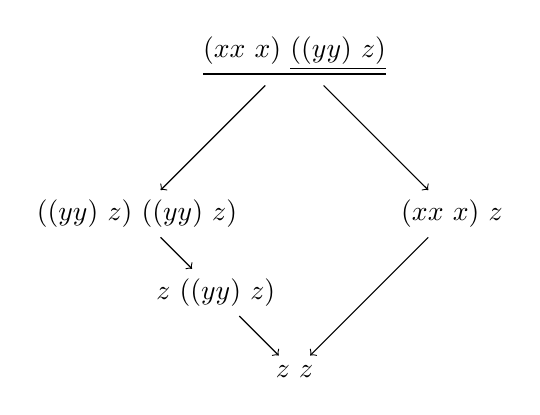
\begin{tikzpicture}
      \node at (0,2)(a){$\underline{(\lam{x}{x\ x})\ \underline{((\lam{y}{y})\ z)}}$};
      \node at (-2,0)(b){$((\lam{y}{y})\ z)\ ((\lam{y}{y})\ z)$};
      \node at (-1,-1)(c){$z\ ((\lam{y}{y})\ z)$};
      \node at (2,0)(d){$(\lam{x}{x\ x})\ z$};
      \node at (0,-2)(e){$z\ z$};

      \draw[->] (a) -- (b);
      \draw[->] (b) -- (c);
      \draw[->] (c) -- (e);
      \draw[->] (a) -- (d);
      \draw[->] (d) -- (e);
      \end{tikzpicture}
    \end{center}

\caption{Counterexample showing that $\beta$-reduction lacks the diamond property.}
\label{fig:betanodia}

\end{figure}

\section{Parallel reduction}

In this section, we define a relation $\Pred^\alpha$ for parallel reduction with renaming\index{parallel reduction}\index{$\Pred^\alpha$}.  This relation will be the desired
intermediate relation between $\abeta$ and $\abeta^*$, with the diamond property.  $\Pred$ is defined
by the rules of Figure~\ref{fig:pred} (i.e., $\Pred$ is the set of pairs $(t,t')$ such that $t\ \Pred\ t'$ has a finite
derivation using those rules).  It allows reduction, in a single step, of any subset of the redexes of the first related term,
to obtain the second.  One could reduce a single redex, several redexes (even nested ones), or no redexes at all.

We then define $\Pred^\alpha$ from $\Pred$ similarly to the way we defined $\betaa$ from
$\betaa_\beta$ (Definition~\ref{def:betaa})\index{$\Pred$}:

\begin{definition}
  $\Pred^\alpha$ is $=_\alpha\Pred $.
\end{definition}
\noindent So one takes an $\alpha$-equivalence step, then a $\Pred$ step.

\newcommand{\predvar}[0]{\infer{x \Pred x}{\ }}

\newcommand{\predlam}[0]{\infer{\lam{x}{t} \Pred \lam{x}{t'}}{t \Pred t'}}

\newcommand{\predapp}[0]{\infer{t_1\ t_2 \Pred t_1'\ t_2'}{t_1 \Pred t_1' & t_2 \Pred t_2'}}

\newcommand{\predbeta}[0]{\infer{(\lam{x}{t_1})\ t_2 \Pred [t_2'/x]t_1'}{t_1 \Pred t_1' & t_2 \Pred t_2'}}

\begin{figure}
\[
\begin{array}{lllllll}
\predvar

& \ &

\predlam

& \ &

\predapp

& \ &

\predbeta
 
\end{array}
\]
\caption{The definition of parallel reduction}
\label{fig:pred}
\end{figure}

Intuitively, we can see that $\Pred$ is intermediate between $\curva_\beta$ and $\curva_\beta^*$, because
it allows reducing any subset of the term's redexes.  Critically, though, it does not allow reduction
of \emph{created redexes}.\index{$\beta$-redex!created}  These are redexes that appear when a variable is replaced by a $\lambda$-abstraction.  For example, we have the reduction
\[
(\lam{x}{x\ y})\ \lam{z}{z}\ \curva_\beta (\lam{z}{z})\ y
\]
\noindent The latter term is a created redex, because there is no corresponding redex in the starting term, from which it is derived.

\subsection{Examples}

Here are some examples of parallel reduction.

\begin{enumerate}
\item Here are all the terms to which $(\lam{x}{x\ x})\ ((\lam{y}{y})\ z)$ parallel reduces:
  \begin{enumerate}
  \item $(\lam{x}{x\ x})\ ((\lam{y}{y})\ z)$, which is the starting term itself;
  \item $(\lam{x}{x\ x})\ z$, where the right redex in the starting term has been contracted;
  \item $((\lam{y}{y})\ z)\ ((\lam{y}{y})\ z)$, where the left redex has been contracted; and
  \item $z\ z$, where both redexes have been contracted.
  \end{enumerate}

  The derivation of the parallel reduction to the last of these is (for an example):

  \[
  \infer{(\lam{x}{x\ x})\ ((\lam{y}{y})\ z) \Pred z\ z}
        {\infer{x\ x \Pred x\ x}{\infer{x \Pred x}{\ } & \infer{x \Pred x}{\ }} & 
          \infer{(\lam{y}{y})\ z \Pred z}
                {\infer{y \Pred y}{\ } &
                  \infer{z \Pred z}{\ }}}
   \]

 \item We have the following parallel reduction:
   \[
   (\lam{x}{\lam{y}{x\ y}})\ (\lam{x}{\lam{y}{x\ y}}) \Pred \lam{y}{(\lam{x}{\lam{y}{x\ y}})\ y}
   \]
   \noindent This same starting term requires $\alpha$-equivalence to reduce further:
   \[
   \begin{array}{ll}
     \underline{(\lam{x}{\lam{y}{x\ y}})\ (\lam{x}{\lam{y}{x\ y}})} &\curva_\beta \\
     \lam{y}{(\lam{x}{\underline{\lam{y}{x\ y}}})\ y} & \curva_a \\
     \lam{y}{\underline{(\lam{x}{\lam{w}{x\ w}})\ y}} & \curva_\beta \\
     \lam{y}{\lam{w}{y\ w}} & \
   \end{array}
   \]
   \noindent But with parallel reduction, as long as all bound variables are distinct from the free variables,
   $\alpha$-equivalence is not required for a single $\Pred$-step.  And a single $\Pred$-step cannot reduce the starting term of this example past where the next redex is created.

\end{enumerate}

\subsection{Properties of parallel reduction}

\begin{lemma}
  \label{lem:predrefl}
  $t \Pred t$ for all terms $t$.
\end{lemma}
\begin{proof}
  The proof is by induction on $t$.

  \case{ } $t$ is a variable $x$. Then we may construct this derivation:
  \[
  \infer{x \Pred x}{\ }
  \]
  
\case{ } $t$ is an application $t_1\ t_2$ for some $t_1$ and $t_2$. Then we may construct:
\[
\infer{t_1\ t_2 \Pred t_1\ t_2}{\infer[\textit{IH}]{t_1 \Pred t_1}{\ } & \infer[\textit{IH}]{t_2 \Pred t_2}{\ }}
\]

\case{ } $t$ is a $\lambda$-abstraction $\lam{x}{t'}$ for some $x$ and $t'$. Then we construct:
\[
\infer{\lam{x}{t'} \Pred \lam{x}{t'}}{\infer[\textit{IH}]{t' \Pred t'}{\ }}
\]
\end{proof}

\begin{lemma}
  \label{lem:betapar}
  $\abeta\ \subseteq\ \Pred^\alpha$.
\end{lemma}
\begin{proof}
  It suffices to assume $t \abeta t'$ for some $t$ and $t'$,
  and show $t \Pred^\alpha t'$.  Since $\abeta$ is defined (Definition~\ref{def:abeta}) to be $\curva_\alpha \cup \curva_\beta$,
  let us consider each possibility.  If we have $t \curva_\alpha t'$, then we have $t \Pred^\alpha t'$, because 
  \begin{enumerate}
  \item $t =_\alpha t'$, and
  \item $t' \Pred t'$, by Lemma~\ref{lem:predrefl}
  \end{enumerate}
  \noindent So we get $t =_\alpha t' \Pred t'$, which suffice to prove $t \Pred^\alpha t'$ (by definition of relational composition).

  Now suppose we have $t \curva_\beta t'$.  Then the proof is by
  induction on the derivation of $t \curva_\beta t'$ (via the rules of
  Figure~\ref{fig:betar}).

  \case{ }
  \[
  \infer{(\lam{x}{t})\ t'\ \curva_\beta\ [t'/x]t}{\ }
  \]
  \noindent We may construct the following, where we invoke Lemma~\ref{lem:predrefl} where indicated, so that we can limit
  the $\beta$-reduction rule for $\Pred$ just to this redex $(\lam{x}{t})\ t'$:
  \[
  \infer{(\lam{x}{t})\ t' \Pred [t'/x]t}
        {\infer[\textit{\ref{lem:predrefl}}]{t \Pred t}{\ } & \infer[\textit{\ref{lem:predrefl}}]{t' \Pred t'}{\ }}
  \]
        

  \case{ }
  \[
  \infer{\lam{x}{t}\ \curva_\beta\ \lam{x}{t'}}{t\ \curva_\beta\ t'}
  \]
  \noindent We construct:
  \[
  \infer{\lam{x}{t} \Pred \lam{x}{t'}}{\infer[\textit{IH}]{t \Pred t'}{t\ \curva_\beta\ t'}}
  \]

  \case{ }
  \[
  \infer{t_1\ t_2\ \curva_\beta\ t_1'\ t_2}{t_1\ \curva_\beta\ t_1'}
  \]
  \noindent Construct the following, again invoking Lemma~\ref{lem:predrefl}:
  \[
  \infer{t_1\ t_2\ \Pred\ t_1'\ t_2}{\infer[\textit{IH}]{t_1 \Pred t_1'}{t_1\ \curva_\beta\ t_1'} &
                                    \infer[\textit{\ref{lem:predrefl}}]{t_2 \Pred t_2}{\ }}
  \]

  \case{ }
  \[
  \infer{t_1\ t_2\ \curva_\beta\ t_1\ t_2'}{t_2\ \curva_\beta\ t_2'}
  \]
  \noindent Similarly to the previous case, construct:
  \[
  \infer{t_1\ t_2\ \Pred\ t_1\ t_2'}{\infer[\textit{\ref{lem:predrefl}}]{t_1 \Pred t_1}{\ }&
                                    \infer[\textit{IH}]{t_2 \Pred t_2'}{t_2\ \curva_\beta\ t_2'} }
  \]
  
        
  \end{proof}

\begin{lemma}
  \label{lem:predmbeta}
  $\Pred^\alpha\ \subseteq\ \abeta^*$
\end{lemma}
\begin{proof}
  Assume $t \Pred^\alpha t'$.  This implies that there exists some $t''$ with
  \[
  t =_\alpha t'' \Pred t'
  \]
  \noindent Since $\abeta$ includes $\curva_\alpha$ by definition, we have
  $t \abeta^* t''$.  So it suffices to show $t'' \abeta^* t'$.  In fact,
  we will show the stronger property $t'' \curva_\beta^* t'$.  This
  is done by  induction on the assumed
  derivation of $t'' \Pred t'$.

  \case{ }
  \[
  \predvar
  \]
  \noindent We construct:
  \[
  \infer{x \betaa_\beta^* x}{\ }
  \]

  \case{ }
  \[
  \predlam
  \]
  \noindent We construct the following, making use of
  Lemma~\ref{lem:comprtc} which implies that the compatible closure of $(\betaa_\beta^*)$
  is the same as just $\betaa_\beta^*$. So the inference at the bottom of the
  derivation, using one of the rules for the compatible closure
  (Figure~\ref{fig:compcl}), is actually a legal inference for
  concluding a $\betaa_\beta^*$ step:
  \[
  \infer[\ref{lem:comprtc}]{\lam{x}{t} \betaa_\beta^* \lam{x}{t'}}
    {\infer[\textit{IH}]{t \betaa_\beta^* t'}{t \Pred t'}}
    \]

    \case{ }
    \[
    \predapp
    \]
    \noindent We construct the following, again applying Lemma~\ref{lem:comprtc}, and ending with transitivity:
    \[
    \infer{t_1\ t_2 \betaa_\beta^* t_1'\ t_2'}
          {\infer[\ref{lem:comprtc}]{t_1\ t_2 \betaa_\beta^* t_1'\ t_2}{\infer[\textit{IH}]{t_1 \betaa_\beta^* t_1'}{t_1 \Pred t_1'}} &
           \infer[\ref{lem:comprtc}]{t_1'\ t_2 \betaa_\beta^* t_1'\ t_2'}{\infer[\textit{IH}]{t_2 \betaa_\beta^* t_2'}{t_2 \Pred t_2'}}}
          \]

    \case{ }
    \[
    \predbeta
    \]
    \noindent We construct the following, again applying Lemma~\ref{lem:comprtc}, and ending with two uses of transitivity.  We assemble proofs about the reductions of $t_1$ and $t_2$, and finish off with a $\beta$-inference.
    \[
    \infer{(\lam{x}{t_1})\ t_2 \betaa_\beta^* [t_2'/x]t_1'}
          {\infer[\ref{lem:comprtc}]{(\lam{x}{t_1})\ t_2 \betaa_\beta^* (\lam{x}{t_1'})\ t_2}
                {\infer[\ref{lem:comprtc}]{\lam{x}{t_1} \betaa_\beta^* \lam{x}{t_1'}}{\infer[\textit{IH}]{t_1 \betaa_\beta^* t_1'}{t_1 \Pred t_1'}}} &
                \infer[\ref{lem:comprtc}]{(\lam{x}{t_1'})\ t_2 \betaa_\beta^* [t_2'/x]t_1'}
                      {\infer[\ref{lem:comprtc}]{(\lam{x}{t_1'})\ t_2 \betaa_\beta^* (\lam{x}{t_1'})\ t_2'}
                        {\infer[\textit{IH}]{t_2 \betaa_\beta^* t_2'}{t_2 \Pred t_2'}}
                     & \infer{(\lam{x}{t_1'})\ t_2' \betaa_\beta^* [t_2'/x]t_1'}{\infer{(\lam{x}{t_1'})\ t_2' \betaa_\beta [t_2'/x]t_1'}{\infer{(\lam{x}{t_1'})\ t_2' \ \beta\  [t_2'/x]t_1'}{\ }}}}}
          \]

          
\end{proof}


\section{Exercises}

\subsection{Confluent terms}

In the following problems, terms $t$, $t_1$, and $t_2$ are given, such
that $t\betaa^* t_1$ and $t\betaa^* t_2$.  Find a term $t'$ such
that $t_1\betaa^* t'$ and $t_2\betaa^* t'$.  You do not have to
write out any reduction sequences.  Please just give the term $t'$.
For fun, you can try to find the minimal such term $t'$, viewing $\betaa$
as an ordering (so try to find $t'$ where there is no other $t''$
satisfying the same property and having $t''\betaa^* t'$) -- but
this is optional.

\begin{enumerate}
\item
\[
  \begin{array}{lll}
    t: & \ & (\lam{x}{x\ (x\ x)})\ ((\lam{y}{y})\ z) \\
    t_1: & \ & z\ (((\lam{y}{y})\ z)\ ((\lam{y}{y})\ z))\\
    t_2: & \ & ((\lam{y}{y})\ z)\ (z\ ((\lam{y}{y})\ z))
  \end{array}
  \]

\item Let $U$ abbreviate $\lam{x}{\textit{true}\ (x\ x)}$.  Recall the definition of the $Y$ combinator from Section~\ref{sec:y}, and \textit{true} from Section~\ref{sec:bool}.
  \[
  \begin{array}{lll}
    t: & \ & Y\ \textit{true} \\
    t_1: & \ & \textit{true}\ (U\ U) \\
    t_2: & \ & \lam{y}{\textit{true}\ (U\ U)}
  \end{array}
  \]
  
\item This problem again uses the $Y$ combinator; recall also \textit{false} from Section~\ref{sec:bool}.  Let
  $U$ abbreviate $\lam{x}{\textit{false}\ (x\ x)\ (\textit{false}\ (x\ x))}$. 
\[
  \begin{array}{lll}
    t: & \ & Y\ (\lam{u}{\textit{false}\ u\ (\textit{false}\ u)}) \\
    t_1: & \ & \textit{id}\ (\textit{false}\ (U\ U)) \\
    t_2: & \ & \textit{false}\ (U\ U)\ \textit{id}
  \end{array}
  \]

\item This problem uses just $\curva_\alpha$ steps:

\[
  \begin{array}{lll}
    t: & \ &   \lam{x}{\lam{y}{x\ \lam{z}{y}}}\\
    t_1: & \ & \lam{x}{\lam{z}{x\ \lam{y}{z}}} \\
    t_2: & \ & \lam{y}{\lam{z}{y\ \lam{y}{z}}}
  \end{array}
  \]

\end{enumerate}

\subsection{Confluence}

\begin{itemize}
  \item Because of our explicit treatment of variable-renaming, single-step $\beta$-reduction with renaming
     ($\betaa$, Definition~\ref{def:betaa}) is not
    confluent. To show this, give an example of a term $t$ and
    distinct normal forms $t_1$ and $t_2$ where $t \curva^* t_1$ and
    $t \curva^* t_2$.

  \item For each of the following relations, argue briefly why it does or does not have the diamond property:
    \begin{itemize}
    \item $\alpha$ (Figure~\ref{fig:barealpha})
    \item $\beta$ (Figure~\ref{fig:barebeta})
    \item $\Tau[\alpha]$ (Figure~\ref{fig:compcl})
    \end{itemize}
    \end{itemize}

\subsection{Parallel reductions}

\begin{enumerate}
\item For each of the following terms, write out all the terms to which they parallel reduce in one step.
  \begin{enumerate}
  \item $\lam{x}{(\lam{y}{y\ y})\ ((\lam{z}{x})\ x)}$
  \item $(\lam{x}{\lam{y}{y\ y}})\ ((\lam{z}{z})\ x)\ \lam{w}{w}$
  \end{enumerate}

\item Let us define a family $I_n$ of terms by recursion on $n\in\mathbb{N}$ (recall that \textit{id} is $\lam{x}{x}$):
  \[
  \begin{array}{lll}
    I_0 & = & \textit{id} \\
    I_{n+1} & = & I_n\ I_n
  \end{array}
  \]
  \noindent So $I_2$, for example, is
  $\textit{id}\ \textit{id}\ (\textit{id}\ \textit{id})$.  Prove by
  induction on $n$ that $I_{n+1} \Pred I_n$.

  \item Give an example of a term $t$ such that $t\ t$ is normalizing but there is no normal term $t'$ such that $t\ t\Pred t'$.

\end{enumerate}





%\chapter{Graph Representations of Lambda Terms}

As we have seen so far, scoping, capture avoidance, and syntactic
substitution have been central technical matters to resolve in
defining lambda calculus.  In this chapter, we explore an alternative
which avoids almost all of that complexity, namely graph
representations of lambda terms.  Instead of representing a term as a
tree, we may represent it as a more general kind of graph.  Instead of
having a name, a binding occurrence of a variable will be represented
by an edge in the graph from the $\lambda$ node to the place the
variable is used.  In order to accommodate terms with multiple bound
occurrences for a particular $\lambda$ node, we must introduce
duplicator nodes that explicitly fork such an edge.  We will make
use of the traditional syntax using bound variables in subsequent
chapters, but it is hopefully enlightening to see this alternative
view.

\subsection{Graphical syntax}

A lambda term in graphical syntax has three kinds of nodes, shown in Figure~\ref{fig:lamgraphs}.  These
may look similar to the tree syntax of Figure~\ref{fig:lamtrees}, but the similarity is superficial.
Here, lambda terms are represented by graphs connecting 

\begin{figure}
\begin{center}
\begin{tabular}{lllll}
  \begin{tikzpicture}
    \node at (0,1.414) (a){\ };
    \node at (1.414,-1.414)(b){\ };
    \node at (-1.414,-1.414)(c){\ };
    \node[circle,draw] at (0,0) (n){$\lambda$};
    \path (n) edge (a)
          edge (b)
          edge (c);
\end{tikzpicture}
&\ \ \ \ \ \ \ &
  \begin{tikzpicture}
    \node at (0,1.414) (a){\ };
    \node at (1.414,-1.414)(b){\ };
    \node at (-1.414,-1.414)(c){\ };
    \node[circle,draw] at (0,0) (n){@};
    \path (n) edge (a)
              edge (b)
              edge (c);
\end{tikzpicture}
  &\ \ \ \ \ \ \  &
  \begin{tikzpicture}
    \node at (0,1.414) (a){\ };
    \node at (1.414,-1.414)(b){\ };
    \node at (-1.414,-1.414)(c){\ };
    \node[regular polygon, regular polygon sides=3,draw] at (0,0) (n){\ };
    \path (n) edge (a)
              edge (b)
              edge (c);
\end{tikzpicture}
\end{tabular}
\end{center}
\caption{The three kinds of nodes for graphical syntax of lambda terms}
\label{fig:lamgraphs}
\end{figure}


\section{Exercises}



\part{Typed Lambda Calculus}

\chapter{Simply Typed Lambda Calculus}

\section{Syntax for types}
\label{sec:synstlc}

We assume a non-empty set $B$ of base types.  These are just any
mathematical objects we wish, that will play the role of atomic
(indivisible) types.  We will use $b$ as a meta-variable for elements
of type $B$.  Similarly as for our metavariables for
$\lambda$-calculus variables (see the start of
Section~\ref{sec:synlam}), we will adopt the convention that different
meta-variables refer to different base types, in any particular
meta-linguistic discussion. \index{base types} The syntax of types is
then:
\[
\textit{simple types}\ T\ ::= \ b\ |\ T \to T'
\]
\noindent There is one parsing convention for simple types, which is
that arrow is right-associative.  So a type like $a \to b \to c$
should be parsed as $a \to (b \to c)$.

Let us consider some examples of simple types.  We might have the type
$\textit{bool} \to \textit{bool}$ for boolean negation, and other
unary (1-argument) boolean operations.  Similarly, a type like
$\textit{bool} \to \textit{bool} \to \textit{bool}$ could describe
conjunction, disjunction, and any other binary boolean operations.
For a higher-order example, a type like $(\textit{nat} \to
\textit{bool}) \to \textit{nat}$ could be the type for a minimization
function \textit{minimize}, where $\textit{minimize}\ p$ returns the
smallest natural number $n$ such that $p\ n$ returns \textit{true}.

Now, it will happen that our notion of typing will not allow
interesting computations with values of atomic types like
\textit{bool}.  So we will not actually be able to type functions like
the ones just described in pure simply typed lambda calculus (STLC).
But STLC is the right framework for characterizing the functional
behavior (via arrow types $T \to T'$) of lambda terms, and thus forms
the core of most other more advanced type systems, including ones
where types like \textit{bool} are definable within the system.

\section{Realizability semantics of types}
\label{sec:stlcrealizability}

One very natural way to understand a type is as a specification
of the behavior of programs.  For example, in a programming
language like Java, suppose a function is declared with the signature

\begin{verbatim}
  int f(int x, int y);
\end{verbatim}

\noindent Then intuitively, the meaning of this is that function
\verb|f| expects two integers \verb|x| and \verb|y| as input and, if
it terminates normally (without raising an exception, diverging,
etc.), then it will return an integer as output.

This idea that a type is a form of specification for programs can be
made precise for STLC using the recursive definition of
Figure~\ref{fig:stlcrealize}.  This defines an interpretation $\interp{T}$ for
any simple type $T$, assuming a function $I$ which interprets the base types of $B$.
The values computed by the semantic function and $I$ are sets of closed terms.  So mathematically,
writing \textit{Types} for the set of all simple types and \textit{ClosedTerms} for the set
of all closed terms of untyped $\lambda$-calculus (and using the standard notation $\mathcal{P} S$ for
the set of all subsets of a set $S$), we have:
\begin{itemize}
\item $\interp{-} \in \textit{Types} \to \mathcal{P}\ \textit{ClosedTerms}$
\item $I \in B \to \mathcal{P}\ \textit{ClosedTerms}$
\end{itemize}

Let us see some examples of this semantics for types.

\begin{figure}
\[
\begin{array}{lll}
\interp{b} & = & I(b) \\
\interp{T_1\to T_2} & = & \{ t\in\textit{ClosedTerms}\ |\ \all{t' \in \interp{T_1}}{(t\ t') \in\interp{T_2}} \}
\end{array}
\]
\caption{Realizability semantics of types, with respect to an assignment $I$ of meanings for base types}
\label{fig:stlcrealize}
\end{figure}

\subsection{Examples and $\beta$-expansion closure}

Suppose that $B$ consists of two base types, $b$ and $b'$.  Let $I(b)$ be the set of Church-encoded booleans,
and let $I(b')$ be the set of Church-encoded natural numbers (see Section~\ref{sec:churchenc}).  Then
certainly we have the following:
\begin{itemize}
\item $\textit{true}\in\interp{b}$
\item $0\in\interp{b'}$
\item $\textit{true}\not\in\interp{b'}$
\end{itemize}

\noindent This looks promising.  But we would expect that with this definition, the negation
function (\textit{not}, of Section~\ref{sec:bool}) on Church-encoded booleans
would be in $\interp{b\to b}$.  But it is not!  The reason is that
\[
\textit{not}\in\interp{b \to b}
\]
\noindent is equivalent, by the second equation of Figure~\ref{fig:stlcrealize}, to
\[
\all{t'\in\interp{b}}{(\textit{not}\ t')\in\interp{b}}
\]
\noindent But $\interp{b}$ does not contain any applications, so it
cannot contain $\textit{not}\ t'$ (since this is an application) for
any $t'$.

The problem here is not in the semantics, but rather the choice of
interpretation function $I$ for the base types.  We will generally
want $I(b)$ to be closed under $\beta$-expansion (Definition~\ref{def:betaexpand}), in the following sense:

\begin{definition}[$\beta$-expansion closed]
  A set $S$ of closed terms is $\beta$-expansion closed if $t\in S$ and $t' \leadsto t$ imply $t' \in S$, for closed $t'$. \index{$\beta$-expansion closed}
\end{definition}

Such a set is closed under $\beta$-expansion in the sense that one cannot leave the
set by following $\beta$-expansion steps to closed terms.  So let us try the example again,
but this time using $\beta$-expansion closed sets (of closed terms) for $I(b)$ and $I(b')$,
namely:
\[
\begin{array}{lll}
  I(b) & := & \{ t\in\textit{ClosedTerms}\ |\ t \leadsto^* \mathbb{B}\} \\
  I(b') & := & \{ t\in\textit{ClosedTerms}\ |\ t \leadsto^* \mathbb{N}\} 
\end{array}
\]
\noindent Here, for brevity, I am writing $t \leadsto^* S$, where $S$
is a set of terms, to mean that there exists $t'\in S$ such that
$t\leadsto^* t'$.  I am also writing $\mathbb{B}$ for the set of
Church-encoded booleans, and $\mathbb{N}$ for the set of
Church-encoded natural numbers.

The facts about meanings of types that we found above still hold for the
$\beta$-expansion closures of the sets of Church-encoded booleans and naturals,
respectively.  But now we can obtain some other interesting facts:
\begin{itemize}
\item $\textit{not}\in\interp{b\to b}$.  To show this, it suffices to
  assume an arbitrary closed $t'$ with $t'\leadsto^*\mathbb{B}$, and show
  that $\textit{not}\ t'\leadsto^*\mathbb{B}$. Suppose $t'\leadsto^*\textit{true}$.
  Then we have
  \[
  \textit{not}\ t' \ \leadsto^*\  \textit{not}\ \textit{true}\ \leadsto^*\ \textit{false}
  \]
  \noindent And similarly, if closed $t'\leadsto^*\textit{false}$, we have
  \[
  \textit{not}\ t' \ \leadsto^*\  \textit{not}\ \textit{false}\ \leadsto^*\ \textit{true}
  \]

\item Let us define this function:
  \[
  \textit{even}\ :=\ \lam{x}{x\ \textit{not}\ \textit{true}}
  \]
  \noindent Given a Church-encoded natural number $n$, this function iterates boolean negation
  $n$ times starting with \textit{true}.  This will result in \textit{true} iff $n$ is indeed even.
  Let us prove that $\textit{even} \in \interp{b' \to b}$.  Assume $t\in\interp{b'}$ and show $\textit{even}\ t \in \interp{b}$.
  Since $t\in\interp{b'}$, there is some natural number $n$ such that
  \[
  t \betaa^* \lam{f}{\lam{x}{\underbrace{f\ \cdots\ (f}_n\ x)}}
  \]
  \noindent Then we have
  \[
  \textit{even}\ t\ \betaeq\ t\ \textit{not}\ \textit{true}\ \betaeq\ \underbrace{\textit{not}\ \cdots\ (\textit{not}}_n\ \textit{true})
  \]
  \noindent We may easily prove that the latter term is $\beta$-equivalent to \textit{true} if $n$ is even, and to \textit{false} if $n$ is odd.

\end{itemize}

\begin{lemma}
\label{lem:betaexpclosed}
  Suppose $I(b)$ is $\beta$-expansion closed, for all $b\in B$. Then $\interp{T}$ is also $\beta$-expansion closed,
  for all $T$.
\end{lemma}
\begin{proof}
  The proof is by induction on $T$.  If $T$ is a base type $b$, then
  $\interp{T} = I(b)$, which is $\beta$-expansion closed by
  assumption.  So assume $T$ is an arrow type $T_1 \to T_2$, and
  assume $t\in\interp{T}$, and closed $t'\betaa^* t$.  We must show
  $t'\in\interp{T}$.  For that, assume $t''\in\interp{T_1}$, and show
  $t'\ t''\in\interp{T_2}$.  By the induction hypothesis, $\interp{T_2}$
  is $\beta$-expansion closed.  So to show $t'\ t''\in\interp{T_2}$,
  it suffices to show that $t\ t''\in\interp{T_2}$, since $t'\ t''$
  reduces to $t\ t''$ (since $t'\betaa^* t$).  But $t\ t''\in\interp{T_2}$
  because $t\in\interp{T_1\to T_2}$ by assumption (and $t''\in\interp{T_1}$).
  \end{proof}

\subsection{Examples with sets of normalizing terms}

Recall that the notation $t \downarrow$
(Definition~\ref{def:normalizing}) means that term $t$ is normalizing:
there exists some $t'$ such that $t\betaa^* t'$ and $t'$ is in normal
form (i.e., does not reduce to any term).

Suppose there is a base type $b\in B$, and define $I(b)$ to be $\{t \in \textit{ClosedTerms}\ |\ t \downarrow\}$.
Then we have:

\begin{itemize}
\item $\lam{x}{\lam{y}{x}} \in \interp{b \to b}$.  To prove this, it suffices by the semantics
  of arrow types to assume $t'\in \interp{b}$, and
  show $(\lam{x}{\lam{y}{x}})\ t' \in \interp{b}$.  Since $\interp{b} = I(b)$,
  we are assuming closed $t' \downarrow$, and need to show $(\lam{x}{\lam{y}{x}})\ t'\downarrow$.
  For the latter:
  \[
  \underline{(\lam{x}{\lam{y}{x}})\ t'} \leadsto \lam{y}{t'}
  \]
  \noindent and the latter is normalizing (and closed) since $t'$ is.

\item Also, $\lam{x}{\lam{y}{x}} \in \interp{b}$, since $\lam{x}{\lam{y}{x}}$ is in normal
  form (and hence normalizing), and closed.

\end{itemize}

With this example, the same term is in $\interp{b}$ and $\interp{b \to b}$.  Here is an example (with the same interpretation $I$ for the base type $b$) where we have a term in $\interp{b}$ that is not in $\interp{b \to b}$:
\begin{itemize}
\item $\lam{x}{x\ x} \in \interp{b}$, since $\lam{x}{x\ x}$ is in normal form and closed.
\item But $\lam{x}{x\ x} \not\in \interp{b \to b}$.  To prove that, we must exhibit $t \in \interp{b}$ such
  that $(\lam{x}{x\ x})\ t$ is not in $\interp{b}$.  We may use $\lam{x}{x\ x}$ for that $t$, because
  we just observed that it is in $\interp{b}$, but $(\lam{x}{x\ x})\ (\lam{x}{x\ x})$ (i.e., the term $\Omega$) is definitely
  not in $\interp{b}$, since $\Omega$ is not normalizing.
\end{itemize}

Now let us change the interpretation $I(b)$ to be $\{ t \in\textit{ClosedTerms}\ |\ t \betaa^* \lam{x}{x}\}$.  Then we
have an example opposite to the one we just found: a term in $\interp{b\to b}$ that is not in $\interp{b}$.
The term is again $\lam{x}{x\ x}$.  This term does not reduce to $\lam{x}{x}$, and so it is not in $\interp{b}$.
But it is in $\interp{b \to b}$.  To show that, assume $t\in\interp{b}$, and show $(\lam{x}{x\ x})\ t\in\interp{b}$.
Since $t\in\interp{b}$, we have $t\betaa^*\lam{x}{x}$.  Then we have the following reduction confirming
that the starting term is in $\interp{b}$:
\[
(\lam{x}{x\ x})\ \underline{t} \leadsto^* \underline{(\lam{x}{x\ x})\ \lam{x}{x}} \leadsto \underline{(\lam{x}{x})\ \lam{x}{x}} \leadsto \lam{x}{x}
\]


\section{Type assignment rules}

To obtain a computable approximation of the realizability semantics of the previous section,
we use a system of rules for deriving facts of the form $\Gamma \vdash t : T$; such facts
are called \emph{typing judgments}\index{typing judgment}.  Here, $\Gamma$
is a \emph{typing context}, with the following syntax:
\[
\textit{typing contexts}\ \Gamma\ ::=\ \cdot\ |\ \Gamma , x : T
\]
\noindent There is an empty context $\cdot$, and a context may be
extended on the right with a binding $x : T$.  This represents an
assumption that $x$ has type $T$.  We will type open terms (terms with
free variable occurrences) by making assumptions, in typing contexts,
about the types of their free variables.  The typing rules are in Figure~\ref{fig:stlctpassign}.

\begin{figure}
\[
\begin{array}{lll}
\infer{\Gamma\vdash x : T}{\textit{Find}\ x:T\ \textit{in}\ \Gamma} 

&

\infer{\Gamma\vdash \lam{x}{t} : T' \to T}
      {\Gamma,x:T'\vdash t:T}

&

\infer{\Gamma\vdash t_1\ t_2 : T}
      {\Gamma\vdash t_1 : T' \to T &
       \Gamma\vdash t_2 : T'}
      \\
      \\

\infer{\textit{Find}\ x:T\ \textit{in}\ (\Gamma, x:T)}{\ }

&

\infer{\textit{Find}\ x:T\ \textit{in}\ (\Gamma, y:T')}{\textit{Find}\ x:T\ \textit{in}\ \Gamma}

&

\ 
\end{array}
\]
\caption{Type-assignment rules for simply typed lambda calculus, with rules for looking up a variable declaration in the context $\Gamma$}
\label{fig:stlctpassign}
\end{figure}

\subsection{Examples}

An example typing derivation is given in Figure~\ref{fig:stlcex}.  Let us adopt the convention that
we do not show derivations of \textit{Find} judgments.  Thus, we will allow derivations to terminate
in applications of the variable rule (first rule in Figure~\ref{fig:stlctpassign}) with premise elided, as long
as that elided premise is actually derivable.

\begin{figure}
  \[
  \infer{\cdot \vdash \lam{x}{\lam{y}{x\ y\ y}} : (b \to b \to b) \to b \to b}
        {\infer{\cdot,x:b \to b \to b \vdash \lam{y}{x\ y\ y} : b \to b}
          {\infer{\Gamma \vdash x\ y\ y : b}
            {\infer{\Gamma \vdash x\ y : b \to b}
              {\infer{\Gamma \vdash x : b \to b \to b}{\ }
              & \infer{\Gamma \vdash y : b}{\ }}
            &\infer{\Gamma \vdash y : b}{\ }}}}
  \]
\caption{Example typing derivation in STLC, where $\Gamma$ abbreviates the typing context $\cdot,x:b \to b \to b, y : b$}
\label{fig:stlcex}
\end{figure}

\subsection{Soundness with respect to the realizability semantics}

We have given two meanings for types, and it is now time to relate
them.  In this section, we will prove soundness of the typing rules
(Figure~\ref{fig:stlctpassign}) with respect to the realizability
semantics (Figure~\ref{fig:stlcrealize}).

In logic generally, suppose we have two ways of defining the meaning
of some formulas, via sets $S_1$ and $S_2$ of formulas that are
considered (by the two semantics respectively) to be true.  Then $S_1$
is sound with respect to $S_2$ iff $S_1 \subseteq S_2$, and $S_1$ is
complete with respect to $S_2$ iff $S_2 \subseteq
S_1$.\index{sound}\index{complete} One way to think about this is as
if $S_1$ consists of statements made by a person, and $S_2$ consists
of statements that are true in reality.  Then soundness means that the
statements the person makes are, in fact, true.  So $S_1$ (the set of
statements the person makes) is a subset of $S_2$ (the statements that
are really true).  Completeness is the inverse of this: if a statement
is really true (i.e., in $S_2$), then the person affirms it (i.e., it
is in $S_1$).  It is easy to be sound: one affirms nothing.  It is
also easy to be complete: one affirms everything.  The ideal, which is
more difficult or even impossible to achieve, depending on the logic,
is to be both sound and complete.

To consider these properties for STLC, we need to formulate the
formulas that our two semantics are affirming.  The basic formula for
typing is $\vdash t : T$.  The corresponding formula for our
realizability semantics is $t \in \interp{T}$.  But the typing rules
make use of typing contexts $\Gamma$ and use more general formulas
$\Gamma \vdash t : T$.  So we will need a corresponding generalization
of the formulas of our realizability semantics.

\begin{definition}
  \label{def:substmodels}
  Define $\interp{\Gamma}$ to be the set of substitutions $\sigma$ such that
  whenever $\textit{Find}\ x:T\ \textit{in}\ \Gamma$ is derivable (with the rules of Figure~\ref{fig:stlctpassign}),
  then $\sigma(x) \in \interp{T}$.
\end{definition}

So $\sigma\in\interp{\Gamma}$ means that the substitution $\sigma$
maps variables to terms that are in the interpretations of the types
that $\Gamma$ says they have.  Let $\sigma\ t$ denote the 
application of the substitution $\sigma$ to $t$, with definition
given in Figure~\ref{fig:substsigma}.  Since we are assuming that the
range of $\sigma$ consists of closed terms (since $\interp{T}$ is a set
of closed terms for every $T$), we do not need to worry
about variable capture: none is possible.

\begin{theorem}
  \label{thm:sltcsnd}
  If $\Gamma\vdash t : T$, then for every $\sigma\in\interp{\Gamma}$, $\sigma\, t \in \interp{T}$,
  for all interpretations $I$ where $I(b)$ is $\beta$-expansion closed.
\end{theorem}
\begin{proof}
  The proof is by induction on the typing derivation.

  \case{ }
\[  \infer{\Gamma\vdash x : T}{\textit{Find}\ x:T\ \textit{in}\ \Gamma} 
\]
Assume $\sigma \in \interp{\Gamma}$.  By definition of the interpretation
of $\Gamma$, this means that $\sigma(x) \in\interp{T}$, and hence $\sigma\,x$, which equals $\sigma(x)$,
is in $\interp{T}$ as required.

  \case{ }
\[  \infer{\Gamma\vdash \lam{x}{t} : T' \to T}
      {\Gamma,x:T'\vdash t:T}
\]
Assume $\sigma\in\interp{\Gamma}$.  To show $\sigma\,\lam{x}{t}\in\interp{T'\to T}$, it suffices
by the definition of substitution and the semantics of arrow types to assume $t'\in\interp{T'}$,
and show that $(\lam{x}{\sigma\, t})\ t'$ is in $\interp{T}$.  Since $\interp{T}$ is $\beta$-expansion closed
by Lemma~\ref{lem:betaexpclosed}, it suffices to show $[t'/x]\sigma\, t\in\interp{T}$.

Let $\sigma'$ be the same as $\sigma$ except that $x$ is mapped to $t'$.
Then $\sigma'\in\interp{\Gamma,x:T'}$, since $\sigma'(x)\in\interp{T}$.  The desired conclusion
now follows directly by the induction hypothesis.
\end{proof}

\begin{figure}
  \[
  \begin{array}{lll}
    \sigma\, x & = & \left\{\begin{array}{ll}
                           \sigma(x),\textnormal{ if }x\in\textit{dom}(\sigma) \\
                           x,\textnormal{ otherwise}
                           \end{array} \right. \\
    \sigma\, (t_1\ t_2) & = & (\sigma\, t_1)\ (\sigma\, t_2) \\
    \sigma\, (\lam{x}{t}) & = & \lam{x}{((\sigma \backslash x)\, t)}
  \end{array}
  \]
  \caption{Applying a substitution of closed terms (thus avoiding danger of variable capture).
    $\sigma \backslash x$ is the function that is just like $\sigma$ except that it does not
  map $x$ to anything.}
  
\label{fig:substsigma}
\end{figure}

 
\section{Relational semantics}

Realizability semantics (Section~\ref{sec:stlcrealizability})
interprets types as sets of terms.  We may also interpret types as
relations on terms.  The definition is in Figure~\ref{fig:relsemstlc},
where we assume now that we have $I \in (B \to
\mathcal{P}\ (\textit{Terms} \times \textit{Terms}))$, and we then
define $\interp{-}\in (\textit{Types} \to \mathcal{P}\ (\textit{Terms}
\times \textit{Terms}))$.  The set $\mathcal{P}\ (\textit{Terms} \times
\textit{Terms})$ is the set of all subsets of the cartesian product
$\textit{Terms} \times \textit{Terms}$.  Since such a subset is just a
relation, we are interpreting base types and then types as relations on
terms.

\begin{figure}
  \[
\begin{array}{lll}
   \interp{b} & = & I(b) \\
   \interp{T_1\to T_2} & = & \{ (t_1,t_2)\ |\ \all{(t', t'') \in \interp{T_1}}{(t_1\ t', t_2\ t'') \in\interp{T_2}} \}
\end{array}
  \]
\caption{Relational semantics of types}
\label{fig:relsemstlc}
\end{figure}

\subsection{Examples}

Suppose we have base types $b$ and $b'$, interpreted as just below.
Recall that $t\ \uparrow$ means that $t$ is not normalizing
(Definition~\ref{def:nonnorm}).  The examples will also use some
defined terms from Chapter~\ref{ch:prog}: $\textit{false}$ for
$\lam{x}{\lam{y}{y}}$, \textit{id} for $\lam{x}{x}$, and $\Omega$ for
the diverging term $(\lam{x}{x\ x})\ \lam{x}{x\ x}$.
\[
\begin{array}{lll}
  I(b) & := & \{ (t,t')\ |\ t \betaeq t' \} \\
  I(b') & := & \{ (t,t')\ |\ t \betaeq t' \betaeq \textit{false} \}
\end{array}
\]
\noindent Then we have the following relational facts:
\begin{itemize}
\item $\lam{x}{x\ \Omega}$ and $\lam{x}{x\ \textit{id}}$ are related
  by $\interp{b' \to b}$.  To prove this using the semantics of
  Figure~\ref{fig:relsemstlc}, we must assume we have terms $t$ and
  $t'$ which are related by $\interp{b'}$, and show that
  $(\lam{x}{x\ \Omega})\ t$ is related to $(\lam{x}{x\ \textit{id}})\ t'$ by
  $\interp{b}$.  Since $\interp{b} = I(b)$, the latter may be shown this
  way:
  \[
  (\lam{x}{x\ \Omega})\ t \ \betaeq \  (\lam{x}{x\ \Omega})\ \textit{false} \ \betaeq \ \textit{false}\ \Omega\ \betaeq\ \textit{id} \ \betaeq\ \textit{false}\ \textit{id}\ \betaeq \ (\lam{x}{x\ \textit{id}})\ \textit{false} \ \betaeq \ (\lam{x}{x\ \textit{id}})\ t'
      \]

 \item That same pair of terms is not related by $\interp{b \to b}$,
      which we can show, by the semantics of Figure~\ref{fig:relsemstlc},
      by finding terms $t$ and $t'$ related by $\interp{b}$, but
      where $(\lam{x}{x\ \Omega})\ t$ and $(\lam{x}{x\ \textit{id}})\ t'$
      are not related by $\interp{b}$.  Take $t$ and $t'$ both to be \textit{id},
      and we have:
     \[
     (\lam{x}{x\ \Omega})\ t\ =\ (\lam{x}{x\ \Omega})\ \textit{id}\ \betaeq\ \Omega \ \neq_\beta\ \textit{id}\ \betaeq\ (\lam{x}{x\ \textit{id}})\ \textit{id}\ = \ (\lam{x}{x\ \textit{id}})\ t'
     \]
     \end{itemize}

\section{The Curry-Howard isomorphism}

Curry observed the deep connection between typed lambda calculus and
logic which, developed further by Howard, is known as the Curry-Howard
isomorphism.  The starting point is to connect STLC with minimal
implicational logic.  This logic is for proving formulas of the
following form, where $p$ is from some nonempty set $P$ of atomic
propositions:
\[
F ::= p\ |\ F_1 \to F_2
\]
\noindent This syntax is the same, disregarding the names of the
metavariables, as that for simple types $T$ (introduced at the start
of Section~\ref{sec:synstlc}).  Figure~\ref{fig:minimpl} gives
inference rules for deriving expressions of the form $S \vdash F$,
where $S$ is a list of formulas, taken as assumptions.  These rules
are (again, disregarding differences in the names of the
meta-variables in question) exactly those of STLC, except without
the terms.

\begin{figure}
\[
\begin{array}{lllll}
\infer{S \vdash F}{\textit{Find}\ F\ \textit{in}\ S}

&\ \ &

\infer{S \vdash F_1 \to F_2}{S , F_1 \vdash F_2}

&\ \ &

\infer{S \vdash F_2}{S \vdash F_1\to F_2 \qquad S \vdash F_1}

\\ \\

\infer{\textit{Find}\ F\ \textit{in}\ (S, F)}{\ }

&\ \ &

\infer{\textit{Find}\ F\ \textit{in}\ (S, F')}{\textit{Find}\ F\ \textit{in}\ S}

&\ \ &

\ 

\end{array}
\]
\caption{Proof rules for minimal implicational logic, with rules for looking up an assumption in a list $S$ of formulas}
\label{fig:minimpl}
\end{figure}

Every STLC typing derivation can be translated to a derivation in
minimal implicational logic, assuming that the set $B$ of base types
in STLC is translated to a subset of the set $P$ of atomic
propositions.  For simplicity, in the following example, let us assume
that $B \subseteq P$ (so the translation is the identity function).
Then we may translate the derivation of Figure~\ref{fig:stlcex} to the
proof in Figure~\ref{fig:minimplex}.  The derivation contains an
unnecessary derivation of $S \vdash b$ from the top to about the
middle of the overall derivation.  It is unnecessary because we can
already derive $S \vdash b$ just using the rule for assumptions (first
rule of Figure~\ref{fig:minimpl}).  Does this mean the correspondence
with the STLC derivation is somehow awry?  Not at all.  For we could
just as well derive $\cdot \vdash \lam{x}{\lam{y}{y}} : (b \to b \to
b) \to b \to b$ in STLC.  The structure of the shorter proof in
minimial implicational logic exactly mirrors this simpler lambda term.

Where one may be content to have proved a theorem without minding
too much the details of the proof, in typed lambda calculus the term
that corresponds to a different proof may be a computationally different
function, as in the example just considered: $\lam{x}{\lam{y}{y}}$
behaves very differently, from a computational perspective, from
$\lam{x}{\lam{y}{x\ y\ y}}$.

\begin{figure}
  \[
  \infer{\cdot \vdash  (b \to b \to b) \to b \to b}
        {\infer{\cdot,b \to b \to b \vdash b \to b}
          {\infer{S \vdash b}
            {\infer{S \vdash b \to b}
              {\infer{S \vdash b \to b \to b}{\ }
              & \infer{S \vdash b}{\ }}
            &\infer{S \vdash b}{\ }}}}
  \]
\caption{Example derivation in minimal implicational logic, where $S$ abbreviates $b \to b \to b, b$}
\label{fig:minimplex}
\end{figure}


\section{Exercises}

\subsection{Realizability semantics for types}

\begin{enumerate}
  
\item Suppose $B$ is $\{ b_1, b_2, b_3\}$, and define $I$, recalling
  from Definition~\ref{def:betanf} that $t\not\betaa$ means that $t$
  is a $\betaa$-normal form:
\begin{eqnarray*}
I(b_1) & = & \{\ t\ |\ \exists t'.\ t\ \betaa^*\ t'\ \betaa\ t'\ \} \\
I(b_2) & = & \{\ t\ |\ \exists t'.\ t \betaa^*\ t'\ \not\betaa \} \\
I(b_3) & = & \{\ t\ |\ \exists t'.\ t \betaa^*\ t'\ \leadsto\ \lam{x}{x} \} \\
\end{eqnarray*}

\noindent Also, define the term $t$ as follows:
\[
t\ =\ \lam{f}{(\lam{x}{x\ x})\ (f\ \lam{x}{x\ x})}
\]

\begin{enumerate}

\item Prove that $t$ is in $\interp{b_2}$.

\item Prove that $t$ is also in $\interp{b_3 \to b_1}$.

\item Prove that $t$ is also in $\interp{(b_2 \to b_3)\to b_3}$.

\item Find a term $t'$ that is in $\interp{(b_3 \to b_2) \to b_2}$
  and also in $\interp{b_1 \to b_1}$; please explain why your term is in both those sets. 

\end{enumerate}
\end{enumerate}
 
\subsection{Type assignment rules}
\label{sec:stlcextp}

\begin{enumerate}

\item Write out typing derivations, using the rules of Figure~\ref{fig:stlctpassign}, for
  the following typing judgments, assuming base types $a$, $b$, and $c$.  You do not need
  to write out the derivations for the \textit{Find} judgment for looking up typings of variables in the
  context.
  \begin{enumerate}
  \item $\cdot, x:b, y : b\to b \vdash y\ (y\ x) : b$
  \item $\cdot \vdash \lam{x}{\lam{y}{x}} : a \to b \to a$
  \item $\cdot \vdash \lam{x}{\lam{y}{\lam{z}{x\ z\ (y\ z)}}} : (a \to b \to c) \to (a \to b) \to a \to c$
  \end{enumerate}
\end{enumerate}  

\subsection{Relational semantics}

\begin{enumerate}
\item Suppose we have a base type $b$, and let $I(b)$ be
  \[
  \{ (t,t')\ |\ (t\ t')\ \downarrow \}
  \]
  \noindent Recall that $t\ \downarrow$ means that $t$ is normalizing (Definition~\ref{def:normalizing}).

  \begin{enumerate}
  \item Argue in detail that $\lam{x}{\lam{y}{x\ (y\ \textit{id})}}$ and $\lam{y}{\lam{z}{z\ y}}$
    are related by $\interp{b \to b}$.

  \item Give another example of a pair of terms in $\interp{b \to b}$.  Please argue in detail for membership in this relation.
  \end{enumerate}
\end{enumerate}

\subsection{Curry-Howard isomorphism}

\begin{enumerate}
\item Translate the typing derivations you did in Section~\ref{sec:stlcextp} above, into proofs in miminal implicational logic.
  \end{enumerate}


\bibliographystyle{plain}
\bibliography{biblio}

\documentclass{book}[12pt]
\usepackage{times}

\usepackage{latexsym}
\usepackage{MnSymbol}
\usepackage{comment}
\usepackage{url}
\usepackage{fullpage}
\usepackage{scrextend}
\usepackage{proof}
\usepackage{array}
\usepackage{xspace}
\usepackage{stmaryrd}
\usepackage{graphicx}
\usepackage{amsmath,amsfonts,amsthm}
\usepackage{makeidx}
\usepackage{float}

\usepackage{tikz}
\usetikzlibrary{arrows}
\usetikzlibrary{shapes}

\usepackage{thmtools}
\declaretheorem[name=Theorem,shaded={},numberwithin=section]{theorem}
\declaretheorem[sibling=theorem]{definition}
\declaretheorem[sibling=theorem]{lemma}
\declaretheorem[sibling=theorem]{corollary}

\usepackage[pdftex,
	pdfauthor={Aaron Stump},
	pdftitle={Introduction to Lambda Calculus},
	colorlinks,
	urlcolor={blue},
	linkcolor={blue},
        citecolor={blue}]{hyperref}

% style for figures
\floatstyle{boxed}
\restylefloat{table}
\restylefloat{figure}


\makeindex

\begin{document}

\title{Introduction to Lambda Calculus}

\author{Aaron Stump \\
Computer Science \\
The University of Iowa
}

\maketitle
\frontmatter

\tableofcontents

\mainmatter

%%%%%%%%%%%%%%%%%%%%%%%%%%%%%%%%%%%%%%%%%%%%%%%%%%%%%%%%%%%%%%%%%%%%%%
% for definitions, proofs, etc.
%%%%%%%%%%%%%%%%%%%%%%%%%%%%%%%%%%%%%%%%%%%%%%%%%%%%%%%%%%%%%%%%%%%%%%

\newcommand{\paradef}[2]{\vspace{#1 cm} %
  \noindent %
  \textbf{#2}}

\newcommand{\case}[1]{\vspace{.1cm} %
  \noindent \underline{Case#1:}}

\newcommand{\todo}[1]{\textbf{[#1]}}

%%%%%%%%%%%%%%%%%%%%%%%%%%%%%%%%%%%%%%%%%%%%%%%%%%%%%%%%%%%%%%%%%%%%%%
% for beta
%%%%%%%%%%%%%%%%%%%%%%%%%%%%%%%%%%%%%%%%%%%%%%%%%%%%%%%%%%%%%%%%%%%%%%

\newcommand{\lam}[2]{\lambda\ #1.\, #2}

% arrows
\newcommand{\curva}[0]{\rightlsquigarrow}
\newcommand{\scurva}[0]{\squigarrowleftright}

% reduction relations
\newcommand{\betar}[0]{\curva_\beta}
\newcommand{\betaa}[0]{\curva}

\newcommand{\Tau}[0]{\mathcal{T}}

%%%%%%%%%%%%%%%%%%%%%%%%%%%%%%%%%%%%%%%%%%%%%%%%%%%%%%%%%%%%%%%%%%%%%%
% for lambda encodings
%%%%%%%%%%%%%%%%%%%%%%%%%%%%%%%%%%%%%%%%%%%%%%%%%%%%%%%%%%%%%%%%%%%%%%

\newcommand{\rep}[1]{\ulcorner #1 \urcorner}

%%%%%%%%%%%%%%%%%%%%%%%%%%%%%%%%%%%%%%%%%%%%%%%%%%%%%%%%%%%%%%%%%%%%%%
% for confluence
%%%%%%%%%%%%%%%%%%%%%%%%%%%%%%%%%%%%%%%%%%%%%%%%%%%%%%%%%%%%%%%%%%%%%%
\newcommand{\Pred}[0]{\Rightarrow}


%%%%%%%%%%%%%%%%%%%%%%%%%%%%%%%%%%%%%%%%%%%%%%%%%%%%%%%%%%%%%%%%%%%%%%
% for STLC
%%%%%%%%%%%%%%%%%%%%%%%%%%%%%%%%%%%%%%%%%%%%%%%%%%%%%%%%%%%%%%%%%%%%%%
\newcommand{\interp}[1]{\llbracket #1 \rrbracket}
\newcommand{\all}[2]{\forall\ #1.\, #2}


\part{Untyped Lambda Calculus}
\chapter{Introduction}

The formal system known as lambda calculus was invented by Alonzo
Church, and published first in his paper ``A Set of Postulates for the
Foundation of Logic''~\cite{church32}.  As that title suggests,
Church's motivation for devising lambda calculus was to create a
formal foundation for logic and mathematics.  This was in response to
the crisis in foundations of mathematics that occurred in the early
20th century, with the discovery of paradoxes in proposed foundational
theories.  Bertrand Russell's discovery, in 1901, of a contradiction
in the foundational theory being developed by Gottlob Frege was a
prime and motivating example~\cite{Whitehead:268025}.  Church's own
theory was quickly discovered to be inconsistent, as, sadly, was even
a revised version~\cite{church33}.  

One may take these failures as as a cautionary tale of the difficulty
of creating consistent foundational theories.  Or, more inspiringly,
one can understand them as showing that many good results can come
from endeavors that fall short of their objectives.  For from these
early systems of Church, and the work he and his brilliant graduate
students carried out consequently, has arisen a remarkable line of
inquiry, with tremendous theoretical and practical impact, on the
subjects of typed and untyped lambda calculus.  For an engaging
exposition of this history, see the paper by Cardone
and Hindley~\cite{cardone09}.

Church subsequently published a research monograph focused on the
lambda calculus as a formal notion of computation, rather than a
foundation for mathematics~\cite{church41}.  I will take this
monograph to be his definitive presentation of lambda calculus.

\subsection{Why this book}

There are a number of very impressive books on lambda calculus
currently available.  For example, Hendrik Barendregt's book remains
an authoritative source for many deep topics in the theory of untyped
lambda calculus~\cite{barendregt85}, and his more recent book,
co-authored with will Dekkers and Richard Statman, is a similar source
for certain topics in typed lambda calculus~\cite{barendregt+13}.  But
these are reference works, which are far too advanced to serve as
textbooks.  One book on lambda calculus that is at an appropriate
level for university instruction is the one by J. Roger Hindley and
Jonathan Seldin~\cite{hindley+08}.  But this book has a more
mathematical perspective on the subject, and puts less emphasis on
certain more computational points.  So in my opinion, there is
currently no available textbook, for students at the late
undergraduate or early graduate level, on lambda calculus from the
perspective of Computer Science.  And that is what the current
volume seeks to supply.

\chapter{Syntax and Reduction Semantics}

\section{The syntax of lambda terms}
\label{sec:synlam}

The untyped lambda calculus has a very small syntax, an appealing
quality for both theoretical study and practical use.  There are just
two syntactic categories: variables and terms.  We assume variables
are taken from some countably infinite set of mathematical objects
(like the natural numbers) disjoint from the other forms of term, and
generally avoid specifying them further.  One stipulation, though is
that whatever variables are, we should be able to test effectively
whether or not two variables are equal.  Such an equality test will be
needed when defining substitution.  We will use $x$ as a meta-variable
for variables, and adopt the convention that in any particular
meta-linguistic discussion, different such meta-variables refer to
different variables.  So if we write $x$ and $y$, please understand
that these meta-variables refer to different actual variables.

Terms are then certain labeled binary trees.  We will use the
meta-variable $t$ (and decorated versions like $t_1$, $t'$, etc.) for
terms.  They are either leaf nodes labeled with variables $x$,
application nodes with subtrees $t_1$ and $t_2$, or lambda nodes with
subtree labeled $x$ and subtree $t'$.  Pictorially, these are shown in
Figure~\ref{fig:lamtrees}.  An application node is said to apply
$t_1$, as a function, to $t_2$, as an argument to that function.  For
a lambda node with subtree labeled $x$ and subtree $t'$, the term $t'$
is called the \emph{body} of the $\lambda$-node.  A term whose root is
labeled $\lambda$ is called a $\lambda$-abstraction.  

\begin{figure}
\begin{center}
\large
\begin{tikzpicture}
  \node at (0,0) {\ }
    child {node {$x$} edge from parent[draw=none]};

  \node at (3,0) {@}
  child { node {$t_1$}}
  child { node {$t_2$}};

  \node at (6,0) {$\lambda$}
  child { node {$x$}}
  child { node {$t'$}};

\end{tikzpicture}
\end{center}
\caption{Graphical depiction of the syntax of terms $t$}
\label{fig:lamtrees}
\end{figure}

While understanding the tree structure for terms is essential for the
study of lambda calculus, it is typical to present terms not as trees,
but textually.  For this, we use the following context-free
grammar, together with two parsing conventions:
\[
\textit{terms}\ t\ ::=\ x\ |\ t_1\ t_2\ |\ \lam{x}{t}\ |\ ( t )
\]
\noindent The parsing conventions are:
\begin{enumerate}
\item Application is left-associative.  So $a\ b\ c$ should be interpreted as $(a\ b)\ c$, as opposed to $a\ (b\ c)$.
\item The scope of $\lambda\ x$ is as far to the right as possible.  So $\lam{x}{x\ x}$ should be interpreted as $\lam{x}{(x\ x)}$, because this grouping shows that the $\lambda\ x$ part of the term governs the application $x\ x$.  This disambiguation is used, instead of $(\lam{x}{x})\ x$.
\end{enumerate}
\noindent Parentheses are just used for disambiguation and do not
correspond to any node in the tree syntax (of
Figure~\ref{fig:lamtrees}).  Figure~\ref{fig:exampleterms} shows
several example terms in both textual form and tree form.  Exercises
below (Section~\ref{sec:extree}) require you to translate between
these forms for some other examples.

\begin{figure}
\large
\begin{center}
\begin{tabular}{llll}

\underline{Textual:} &
$\lam{x}{x}$ &
$x\ \lam{x}{x\ x}$ &
$\lam{x}{\lam{y}{y\ x\ x}}$

\\ 
\underline{Disambiguated:} &
$\lam{x}{x}$ &
$x\ \lam{x}{(x\ x)}$ &
$\lam{x}{\lam{y}{((y\ x) x)}}$

\\ 

\begin{tikzpicture}
  \node at (0,0) {\underline{Tree:}}
  child { node {\ } edge from parent[draw=none]
    child { node {\ } edge from parent[draw=none]
      child { node {\ } edge from parent[draw=none]
        child { node {\ } edge from parent[draw=none]}}}};
\end{tikzpicture}

\vspace{1cm}
&

\begin{tikzpicture}
  \node at (0,0) {$\lambda$}
  child { node {$x$}}
  child { node {$x$}
    child { node {\ } edge from parent[draw=none]
      child { node {\ } edge from parent[draw=none]
        child { node {\ } edge from parent[draw=none]
}}}};
\end{tikzpicture}

&

\begin{tikzpicture}
  \node at (0,0) {@}
  child { node {$x$}}
  child { node {$\lambda$}
    child { node {$x$}}
    child { node {@}
      child { node {$x$} }
      child { node {$x$}
      child { node {\ } edge from parent[draw=none]}}}};
\end{tikzpicture}

&

\begin{tikzpicture}
  \node at (0,0) {$\lambda$}
  child { node {$x$}}
  child { node {$\lambda$}
    child { node {$y$}}
    child { node {@}
      child { node {@}
        child {node {$y$}}
        child {node {$x$}}}
      child { node {$x$}}}};
\end{tikzpicture}

\\


\end{tabular}

\end{center}
\caption{Some example terms, in textual form (where parsing conventions must be applied), then disambiguated textual form (no parsing conventions needed), and finally tree form}
\label{fig:exampleterms}
\end{figure}

\begin{definition}[subterm]
  A subterm of a term $t$ is just some subtree (possibly $t$ itself) of $t$.\index{subterm}
  \end{definition}

\section{Binding, bound, and free variable occurrences}

As will become more apparent shortly, the $\lambda$ symbol introduces
its variable $x$ \emph{locally} in the body.  This means that this $x$
used in the body of a $\lambda$-abstraction is semantically different
from the same variable $x$ used outside the body.  In Computer Science
terms, $\lambda$ introduces $x$ as a local variable, whose scope
(i.e., the part of the expression where this variable introduction is
in force) is the body of the $\lambda$-abstraction.

The following basic terminology is used to describe occurrences of a
variable $x$; i.e., nodes in term (in tree form) labeled by a
variable.  If the occurrence is the left child of a $\lambda$-node,
then this is called a \emph{binding} occurrence\index{variable!binding
  occurrence}.  If the occurrence is somewhere inside the right
subtree of a $\lambda$-node introducing $x$, then the occurrence is
called \emph{bound}\index{variable!bound occurrence}.  And finally, if
the variable occurrence is neither binding nor bound it is called
\emph{free}\index{variable!free occurrence}: it is not in the scope of
a $\lambda$-node binding $x$.  It is common to write $\textit{FV}(t)$
for the set of variables with free occurrences in $t$\index{FV}.  See
Figure~\ref{fig:varocc} for an example illustrating this terminology.
A term with at least one free variable occurrence is called \emph{open}\index{term!open},
and a term with no free variable occurrences is called \emph{closed}\index{term!closed}.

\begin{figure}
\large
\begin{center}
    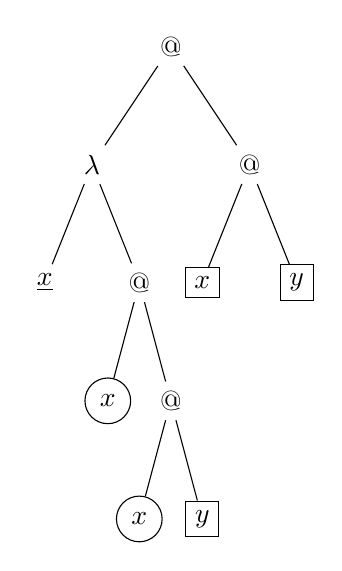
\begin{tikzpicture}
      [level 1/.style={sibling distance=20mm},
        level 2/.style={sibling distance=12mm},
          level 3/.style={sibling distance=8mm}]
      \node at (0,0) {@}
            child { node {$\lambda$}
              child { node {\underline{$x$}}}
              child { node {@}
                child { node [draw,circle] {$x$}}
                child { node {@}
                  child { node[draw,circle] {$x$}}
                  child { node[draw,rectangle] {$y$}}
}}}
            child { node {@}
              child {node[draw,rectangle] {$x$}}
              child {node[draw,rectangle] {$y$}}};
    \end{tikzpicture}
    \end{center}
    \caption{Example term illustrating the concepts of binding, bound, and free variable occurrence.  The underlined node is a binding occurrence, circled nodes are bound occurrences (bound by that sole underlined binding occurrence), and boxed nodes are free occurrences.}
    \label{fig:varocc}

\end{figure}

\section{Capture-avoiding substitution}
\label{sec:subst}

To define how $\lambda$-terms compute (Section~\ref{sec:singlebeta}
below), we need a notion of substitution, where one term $t'$ is
substituted for the free occurrences of a variable $x$ in another term
$t$.  We will use the notation $[t'/x]t$ to denote the result of this
substitution, if defined\index{substitution!capture-avoiding}.
Substitution is used to define how lambda abstractions reduce (i.e.,
compute) when applied to arguments.  We will need to substitute
arguments $t'$ for input variables $x$ in bodies $t$ of
$\lambda$-abstractions.  Note that the notation $[t'/x]t$ is part of
our meta-language discussion of $\lambda$-calculus, and not new
object-language syntax within the language of $\lambda$-calculus.
Also, it should be mentioned that one finds numerous other notations
for substitution in the literature.  For example, Church writes
$\textsf{S}^x_{t'} t$ where we are instead writing $[t'/x]t$.

Defining substitution is, arguably, the central technical issue
in the definition of the lambda calculus.  The problem is essentially
one of the proper maintenance of scoping of variable, as we will
consider next.

\subsection{Variable capture}

 The main problem in defining substitution is to ensure that a
 substitution $[t'/x]t$ avoids \emph{variable capture}, where some
 free occurrences of a variable $y$ in the term $t'$ get captured by a
 $\lambda$-abstraction of $y$ occurring in $t$.  Such a capture would
 represent a change of scoping of those occurrences in $t'$: before
 the subsitution, they were not bound by any $\lambda$-abstraction in
 $t$, but after the substitution they are.  This change of scoping is
 to be prevented.

 The simplest example of the problem is $[y/x]\lam{y}{x}$.  A naive
 (and scope-incorrect) approach to substitution would produce $\lam{y}{y}$.
 But then the occurrence of $y$ that is being substituted has changed its scoping.  Before the
 substitution, it is not bound by the displayed $\lambda\ y$, but after the
 substitution, it is.  So it has been captured.

 It is common practice, in many research works, to deal with the
 problem of variable capture by assuming that variables are implicitly
 renamed to avoid capture.  So for this example, the common practice
 would be to say that the result of $[y/x]\lam{y}{x}$ is $\lam{w}{y}$,
 for some variable $w$ different from $x$ and $y$.  This is the
 approach taken in Hindley and Seldin's book, where it is even
 specified which variable $w$ (from the countably infinite supply of
 variables) is to be used~\cite{hindley+08}.  So substitution, in
 Hindley and Seldin, is indeed a function; not all authors are so
 careful.  Additionally, most works assume what is known as
 Barendregt's variable convention: in discussing some finite set of
 lambda terms, we assume that no variable occurs both free in one of
 the terms and bound in one of the terms~\cite[Definition
   2.1.13]{barendregt85}, and further assume that variables are
 implicitly renamed to ensure this.

 In this book, I will follow a different approach, adopting a modified
 version of Church's original proposal for dealing with renaming of
 variables~\cite{church41}.  During reduction, substitution is not
 allowed in case it would lead to capture, and variables must be
 explicitly renamed first in additional reduction steps.  I have
 several reasons for pursuing this approach.  First, as variable
 binding is one of the central technical issues of lambda calculus, it
 is better, certainly when first learning the theory, not too try to
 ignore the problem by assuming things are arranged so that it never
 arises.  Second, variable binding turns out to be one of the most
 tricky aspects both for implementation of languages incorporating
 lambda calculus, and for formalizing the meta-theory of such
 language in computer theorem-proving systems.  So again, dealing with
 the problem head-on seems best, as it may encourage development of the theory
 in a way that minimizes, rather than ignores, the issue.  Perhaps
 we will find better ways to formalize lambda calculus if we isolate
 the places where renaming is needed, for example.  And finally,
 some research is directly concerned with issues of renaming
 in lambda calculus, and thus needs to be completely explicit about
 the issue.  An example is works seeking to analyze when renaming
 can always be avoided~\cite{vanoostrom23}.


\subsection{Substitution as a partial function}

Figure~\ref{fig:subst} gives the definition of substitution as a
partial function.  Recall the meta-variable convention that $x$ and
$y$ are assumed to refer to different object-language variables.  In
Equations 3 and 4 it is intended (by the ``otherwise'' at the end of Equation 2)
that $x\in\textit{FV}(t_1\ t_2)$ and $x\in\textit{FV}(\lam{y}{t})$,
respectively.  This ensures that at most one equation can be
instantiated to obtain a fact about substitution $[t_1/x]t_2$, for any
particular $t_1$, $x$, and $t_2$.  For Equations 3 and 4, let us
understand that if the right-hand side of the equation is undefined
(in some instance of the equation), then the left-hand side is, too.

\begin{figure}
\large
\[
  \begin{array}{llll}
1. &    [t'/x]x & = & t' \\
2. &    [t'/x]t & = & t, \textnormal{if }x\not\in\textit{FV}(t); \textnormal{otherwise:} \\
3. &    [t'/x](t_1\ t_2) & = & ([t'/x] t_1)\ [t'/x]t_2 \\
4. &    [t'/x]\lam{y}{t} & = & \lam{y}{[t'/x]t}, \textnormal{if } y \not\in\textit{FV}(t')
  \end{array}
\]
  \caption{Recursive definition of capture-avoiding substitution as a
    partial function.  If a recursive call is undefined then the outer
    call is also considered undefined.  The case that is similar to
    the last clause of the definition but where $y\in\textit{FV}(t')$
    is the basic undefined case.  The clauses (equations) of the definition are numbered for reference later.}
  \label{fig:subst}
  \end{figure}

\subsection{Examples}

Here are some examples of capture-avoiding substitution.

\begin{enumerate}
\item $[\lam{x}{x}/y]\lam{z}{y\ z} = \lam{z}{(\lam{x}{x})\ z}$.  In detail, labeling the equality symbol with the number of the clause from Figure~\ref{fig:subst}, and underlining the part of the term that is being changed (just for clarity), the calculation is:

  \[
  \begin{array}{ll}
    \underline{[\lam{x}{x}/y]\lam{z}{y\ z}} & =_4 \\
    \lam{z}{\underline{[\lam{x}{x}/y](y\ z)}} & =_3 \\
    \lam{z}{\underline{([\lam{x}{x}/y]y)}\ [\lam{x}{x}/y]z} & =_1 \\
    \lam{z}{(\lam{x}{x})\ \underline{[\lam{x}{x}/y]z}} & =_2 \\
    \lam{z}{(\lam{x}{x})\ z} & \
  \end{array}
  \]

\item $[(x\ x)/y]\lam{y}{x\ y} = \lam{y}{x\ y}$.  This is just by clause 2 of Figure~\ref{fig:subst}, because we are substituting for variable $y$ in a $\lambda$-abstraction which binds $y$.  The $y$ for which we are substituting cannot possibly occur free in a $\lambda$-abstraction of $y$, so substitution stops, returning the term (into which we are trying to substitute) unchanged.

\item $[\lam{y}{x\ y}/z](z\ \lam{x}{x}) = (\lam{y}{x\ y})\ \lam{x}{x}$.  In detail, we have
  \[
    \begin{array}{ll}
      \underline{[\lam{y}{x\ y}/z](z\ \lam{x}{x})} & =_3 \\
      (\underline{[\lam{y}{x\ y}/z]z})\ [\lam{y}{x\ y}/z]\lam{x}{x} & =_1 \\
      (\lam{y}{x\ y})\ \underline{[\lam{y}{x\ y}/z]\lam{x}{x}} & =_2 \\
      (\lam{y}{x\ y})\ \lam{x}{x} & \ 
    \end{array}
    \]

  \item The substitution $[x\ x/y]\lam{x}{y\ y}$ is undefined, because
    to push the substitution inside a $\lambda$-abstraction, clause 4
    of Figure~\ref{fig:subst} requires that the $\lambda$-bound
    variable (in this case $x$) is not free in the term we are
    substituting (which here is $x\ x$).  Since $x$ is free in $x\ x$,
    this means we cannot apply any of the equations of Figure~\ref{fig:subst}
    and the substitution is undefined.
\end{enumerate}

\subsection{Some properties of capture-avoiding substitution}

The following lemmas are used below.  The proofs are a bit technical, carefully applying
the definition of substitution from Figure~\ref{fig:subst}.  Dealing with the possibility
that substitutions are undefined is a somewhat tedious necessity.  Each lemma is presented
with an example, before its proof.

\begin{lemma}
\label{lem:substvargone}
  Suppose that $x\not\in\textit{FV}(t_1)$, and $[t_1/x]t_2$ is defined.  Then
  $x\not\in\textit{FV}([t_1/x]t_2)$.
\end{lemma}

\noindent\textit{Intuitive idea.} Substitution of a term $t_1$ for a variable $x$ in term $t_2$ results in a term
with no free occurrences of
$x$ (since they have all been replaced by substitution), as long as $x$ is not free in the substituted term $t_1$.

\vspace{.2cm}

\noindent\textit{Example.} Take $t_1$ to be $\lam{y}{y}$, and $t_2$ to be $x\ \lam{z}{z}$.
The conditions of the lemma are satisfied, and the result of applying the substitution
is $(\lam{y}{y})\ \lam{z}{z}$.  As stated in the lemma, $x$ does not occur free in this term.

\vspace{.2cm}

\noindent\textit{Example where the first condition does not hold.} If
we take $t_1$ to be $\lam{y}{x}$, and $t_2$ to be $x\ \lam{z}{z}$,
then the result of applying the substitution is
$(\lam{y}{x})\ \lam{z}{z}$, which does contain $x$ free.  Hence, the first condition is needed.

\begin{proof} The proof is by induction on $t_2$.
  If $x\not\in\textit{FV}(t_2)$, then by Equation 2 of Figure~\ref{fig:subst}, $[t_1/x]t_2 = t_2$, and
  hence $x\not\in\textit{FV}([t_1/x]t_2)$ (since $[t_1/x]t_2 = t_2$ and we are assuming $x\not\in\textit{FV}(t_2)$).
  So suppose $x\in\textit{FV}(t_2)$. If $t_2$ is $x$, then $[t_1/x]t_2 = t_1$,
  and the result follows by the assumption that $x\not\in\textit{FV}(t_1)$.
  If $t_2$ is $t_a\ t_b$ for some terms $t_a$ and $t_b$,
  then by the induction hypothesis, $x\not\in\textit{FV}([t_1/x]t_a)$ and $x\not\in\textit{FV}([t_1/x]t_b)$.
  So $x\not\in\textit{FV}([t_1/x](t_a\ t_b))$, since $[t_1/x](t_a\ t_b) = ([t_1/x]t_a)\ [t_1/x]t_b$ by Equation 3 of Figure~\ref{fig:subst}.
  If $t_2$ is $\lam{z}{t}$ for some $t$ and some $z$ different from $x$,
  then by the induction hypothesis, $x\not\in\textit{FV}([t_1/x]t)$.  So $x\not\in\textit{FV}(\lam{z}{[t_1/x]t})$.  The
  latter expression
    equals $[t_1/x]\lam{z}{t_2}$, since the substitution is assumed to be defined.
\end{proof}


\begin{lemma}
\label{lem:substundo}
  Suppose that $y\not\in\textit{FV}(t)$, and $[y/x]t$ is defined.  Then
  $[x/y][y/x]t$ is defined and equals $t$.
\end{lemma}

\noindent\textit{Intuitive idea.} Substituting variable $y$ for
variable $x$ and then reversing that (to substitute $x$ for $y$)
leaves the term unchanged, as long as it is legal to replace $x$ with
$y$ (avoiding capture), and as long as the original term does not have any free $y$ (since then substituting $x$ for $y$ would replace those free occurrences of $y$ with free occurrences of $x$, and the term would be different in the end).

\vspace{.2cm}

\noindent\textit{Example.} If we substitute $y$ for $x$ in $x\ \lam{x}{x}$, we get $y\ \lam{x}{x}$.  Then substituting $x$ for
$y$ restores the original term $x\ \lam{x}{x}$.

\begin{proof}
  The proof is by induction on $t$.  If $t$ is $x$, then $[x/y][y/x]x = x$.  If $x\not\in\textit{FV}(t)$,
  then $[x/y][y/x]t = [x/y]t$.  Furthermore, since $y\not\in\textit{FV}(t)$ by assumption, we have $[x/y]t = t$.
  For the rest of the proof, then, suppose $x\in\textit{FV}(t)$.

  If $t$ is $t_1\ t_2$ for some $t_1$ and $t_2$, then by the semantics of Figure~\ref{fig:subst},
  the expressions $[x/y][y/x](t_1\ t_2)$ and $([x/y][y/x]t_1)\ [x/y][y/x]t_2$ are either (a) both undefined
  or else (b) both defined and equal. Since $[y/x](t_1\ t_2)$ is defined, so are $[y/x]t_1$ and $[y/x]t_2$.
  By the induction hypothesis, then, $[x/y][y/x]t_1$ and
  $[x/y][y/x]t_2$ are defined and equal $t_1$ and $t_2$, respectively.  So $[x/y][y/x]t_1\ [x/y][y/x]t_2$ is defined and
  equals $t_1\ t_2$.  This means that it must have
  been option (b).  So $[x/y][y/x](t_1\ t_2)$ must be defined and equal to that same value, namely $t_1\ t_2$.

  Now suppose $t$ is a $\lambda$-abstraction of some variable different from $x$ (as the
  case where it is an abstraction of $x$ is covered above, by the reasoning when $x\not\in\textit{FV}(t)$).
  It is also not possible for $t$ to be $\lam{y}{t'}$ for any $t'$, because if the bound variable is $y$, the substitution
  $[y/x]\lam{y}{t'}$ is undefined, 
  So the only case we must consider is where $t$ is $\lam{z}{t'}$ for some $z$ (different from $x$ and $y$) and $t'$.

  We wish to apply the induction hypothesis to conclude that $[x/y][y/x]t'$ is defined and equals $t'$.  For this,
  we need to know first that $y\not\in\textit{FV}(t')$.  But this follows from the facts that $y\not\in\textit{FV}(\lam{z}{t'})$
  and $y \neq z$.  Second, we need to know that $[y/x]t'$ is defined.  But this follows since $[y/x]\lam{z}{t'}$ is
  defined and equals $\lam{z}{[y/x]t'}$.  Since that expression is defined, so also
  must its subexpression $[y/x]t'$ be defined.  So we can indeed apply the induction hypothesis to conclude
  that $[x/y][y/x]t'$ is defined and equals $t'$.

  Now again by the semantics of Figure~\ref{fig:subst}, since $z$ is different from $x$ and $y$, either $[x/y][y/x]\lam{z}{t'}$
  and $\lam{z}{[x/y][y/x]t'}$ are both undefined, or else both defined and equal.  But the reasoning of the previous
  paragraph shows that $\lam{z}{[x/y][y/x]t'}$ is defined (since we concluded that $[x/y][y/x]t'$ is defined)
  and equals $\lam{z}{t'}$ (since we concluded $[x/y][y/x]t' = t'$ by induction hypothesis).  Hence, $[x/y][y/x]\lam{z}{t'}$
  is also defined, and equals $\lam{z}{t'}$, as required.
\end{proof}

\section{Single-step beta-reduction}
\label{sec:singlebeta}

The central computational concept in $\lambda$-calculus is
\emph{$\beta$-reduction}, which explains how to evaluate function
calls.  A function call is an application of a $\lambda$-abstraction
to an argument.  So as a tree, it looks like:
\begin{center}
\begin{tikzpicture}
  \node at (0,0) {@}
  child { node {$\lambda$}
    child { node {$x$}}
    child { node {$t$} }}
  child { node {$t'$}};
\end{tikzpicture}
\end{center}
\noindent In textual form, it is $(\lam{x}{t})\ t'$.  The
$\beta$-axiom says that such a term reduces to $[t'/x]t$; i.e., the
result of substituting $t'$ for $x$ in
$t$, as discussed in Section~\ref{sec:subst} above.  This is only
allowed, however, if the substitution is defined.  Operationally, this
reduction of the $\beta$-redex to the result of a substitution is
called \emph{contracting} the redex; the result of substitution is called
the \emph{contractum}
\index{$\beta$-redex!contracting}\index{contractum}.  Terms of the
form $(\lam{x}{t})\ t'$, with $[t'/x]t$ defined, are called
$\beta$-redexes (for ``$\beta$-reducible
expressions'')\index{$\beta$-redex}.  Note that the requirement that
the substitution is defined is a particularity of the approach we take
in this book.

To give a formal definition of $\beta$-reduction, we will first define
what it means to reduce a single $\beta$-redex, and then, in
Section~\ref{sec:multibeta} below, define $\beta$-reduction with
multiple steps.  In both cases, we define relations between terms.  For
single-step $\beta$-reduction, the relation is denoted $\curva_\beta$.

You may recall that set theoretically, a relation is just a set of
ordered pairs, and we may equivalently write $(t,t')\in\curva$ or $t
\curva t'$ to indicate that $t$ $\beta$-reduces to $t'$.  There are
several ways to give the definition, and we will consider two.
First, we can define the $\beta$-reduction relation using a set of inference rules\index{inference rule}.
Such rules are of the form
\[
\frac{\textit{premise}_1 \ \ \cdots \ \ \textit{premise}_n}{\textit{conclusion}}
\]
\noindent It is allowed for $n$ to be $0$, in which case there are no
premises and the rule is called an \emph{axiom}.  Inference rules are
to be understood as universally quantified implications: the
conjunction of the premises implies the conclusion, for all
instantiations of the meta-variables used.  A \emph{derivation} is a
kind of tree built by instantiating the inference rules in various
ways, and then using the conclusion of one inference as the premise of
another\index{derivation}.  Such instantiated inference rules are
called \emph{inferences}\index{inference}.  A derivation is
\emph{open} if there are some premises that are not the conclusion of
any inference\index{derivation!open}.  Otherwise, it is called
\emph{closed}\index{derivation!closed}. We further stipulate that we
are only interested in facts that can be proved using finite
derivations.  

A definition of $\beta$-reduction using inference rules is given in
Figure~\ref{fig:betar}.  The leftmost rule in the figure is the
$\beta$ rule, where we require that $[t'/x]t$ is defined
in order to use the rule for inferences in a derivation.  The other
three rules express the idea that a reduction can take place anywhere
in a term.  Figure~\ref{fig:betarex} gives some example derivations.

\begin{definition}[Single-step $\beta$-reduction (rules)]
\label{def:beta}
The relation $\curva_\beta$ is the set consisting of exactly those
pairs $(t,t')$ where $t \curva_\beta t'$ is derivable (via a finite derivation) using the
rules of Figure~\ref{fig:betar}.  We write applications of the
relation in infix notation (as in those rules).  If $t \curva_\beta t'$
we say that $t$ $\beta$-reduces to $t'$.  
\end{definition}

\begin{definition}[$\beta$-redex]
  Any term of the form $(\lam{x}{t})\ t'$ is called a $\beta$-redex,
  as long as $[t'/x]t$ is defined.  Otherwise, we call such a term
  a \emph{stuck} $\beta$-redex.\index{$\beta$-redex!stuck}\index{$\beta$-redex}
  \end{definition}

\begin{definition}[nested redex]
  Suppose that a redex $R_1$ is a subterm of some other redex $R_2$.
  Then we say that $R_1$ is a nested redex (nested within $R_2$).
  \end{definition}
 
\begin{definition}[$\beta$-expansion]
\label{def:betaexpand}
  The inverse of the $\leadsto_\beta$ relation is called
  $\beta$-expansion.  If $t \leadsto_\beta t'$, we say
  that $t'$ $\beta$-expands to $t$.\index{$\beta$-expansion}
\end{definition}

\begin{figure}
  \[
  \begin{array}{lllllll}
\infer{(\lam{x}{t})\ t'\ \curva_\beta\ [t'/x]t}{\ } & \ &
\infer{\lam{x}{t}\ \curva_\beta\ \lam{x}{t'}}{t\ \curva_\beta\ t'} & \ &
\infer{t_1\ t_2\ \curva_\beta\ t_1'\ t_2}{t_1\ \curva_\beta\ t_1'} &\ &
\infer{t_1\ t_2\ \curva_\beta\ t_1\ t_2'}{t_2\ \curva_\beta\ t_2'}
  \end{array}
  \]
  \caption{Inference rules defining the $\beta$-reduction relation.  It is required that the substitution in the leftmost rule be defined, in order to use the rule.}
  \label{fig:betar}
\end{figure}

\begin{figure}
  \[
  \begin{array}{lll}
    \infer{(\lam{x}{x\ x})\ \lam{y}{y} \betar (\lam{y}{y})\ \lam{y}{y}}
          {\ }
    &
    \infer{\lam{x}{(\lam{y}{y})\ x} \betar \lam{x}{x}}
          {\infer{(\lam{y}{y})\ x \betar x}{\ }}

    &

    \infer{x\ (y\ ((\lam{x}{x})\ z)) \betar x\ (y\ z)}
          {\infer{y\ ((\lam{x}{x})\ z) \betar y\ z}
            {\infer{(\lam{x}{x})\ z \betar z}{\ }}}
  \end{array}
\]
\caption{Example derivations using the rules of Figure~\ref{fig:betar} for $\beta$-reduction.}
\label{fig:betarex}
\end{figure}

\noindent The following definition is generic, for any $R\subseteq (A\times A)$.  We will call such
a set a (binary) relation on $A$.\index{binary relation on a set}

\begin{definition}[determinism]
\label{def:det}
  An element $x$ is said to be deterministic with respect to some
  relation $R$ on a set $A$ iff for all $y$ and $y'$, if $x R y$ and
  $x R y'$ then $y = y'$.  $R$ itself is called deterministic iff
  every element of $A$ is deterministic with respect to $R$.
  Mathematically, being deterministic is the same as being a
  functional relation.  A nondeterministic relation is then simply one
  which fails to be deterministic for at least one
  $x$.\index{relation!deterministic}\index{determinism}
  \end{definition}

\begin{lemma}
  The $\leadsto_\beta$ relation is nondeterministic.
\end{lemma}
\begin{proof}
  Any term containing two non-nested $\beta$-redexes will have
  two distinct contracta.  For example, $(\lam{x}{x}\ y)\ (\lam{x}{x}\ z)$
  has distinct contracta $y\ (\lam{x}{x}\ z)$ and $(\lam{x}{x}\ y)\ z$.
  Hence, $\leadsto_\beta$ is nondeterministic.
\end{proof}

\subsection{An alternative definition using contexts}

Another way to define the same $\curva_\beta$ relation is with
contexts.  Let us first introduce the concept of \emph{grafting},
which is just substitution that does \underline{not} avoid
capture\index{grafting}.  We will write $\langle t/x\rangle t'$ for
the grafting relation (there does not seem to be a generally adopted
notation for grafting).  The definition, given in
Figure~\ref{fig:grafting}, is essentially the same as the one for substitution,
except that the last clause does not impose
any requirements on $\textit{FV}(t')$.

\begin{figure}
\large
\[
  \begin{array}{lll}
\    \langle t'/x \rangle x & = & t' \\
\    \langle t'/x \rangle t & = & t, \textnormal{if }x\not\in\textit{FV}(t); \textnormal{otherwise:} \\
\    \langle t'/x \rangle(t_1\ t_2) & = & (\langle t'/x\rangle t_1)\ \langle t'/x\rangle t_2 \\
\    \langle t'/x\rangle\lam{y}{t} & = & \lam{y}{\langle t'/x\rangle t}
  \end{array}
\]
  \caption{Recursive definition of grafting, a total function similar to substitution but intentionally allowing variable capture.}
  \label{fig:grafting}
  \end{figure}

\begin{definition}[context]
  A term $t$ is called a context iff it contains exactly one free
  occurrence of a special fixed variable $q$\index{context}.  If $t$
  is a context, then we write $\langle t'/q \rangle t$ more briefly as
  $\langle t' \rangle t$.
  \end{definition}

\noindent Using contexts, we may give the following alternative definition of the $\beta$-reduction relation:

\begin{definition}[Single-step $\beta$-reduction (contexts)]
\label{def:betactxt}
The single-step $\beta$-reduction relation
$\curva_\beta$ is alternatively defined to be the set of all ordered pairs with first component $\langle (\lam{x}{t})\ t' \rangle t''$
  and second component $\langle [t'/x]t \rangle t''$, for some $x$, $t$, $t'$, and $t''$ (with $t''$ a context and $[t'/x]t$ defined).
\end{definition}

The idea of this definition is to express that (in operational terms)
if you find a $\beta$-redex somewhere in some possibly bigger term
$t_1$, then you may reduce $t_1$ by contracting that $\beta$-redex and
then rebuilding the rest of the term $t_1$ around the contractum.  The
definition expresses finding $(\lam{x}{t})\ t'$ in possibly bigger
term $t_1$ by writing $\langle(\lam{x}{t})\ t'\rangle t''$ for $t_1$.
In other words, you have some term $t_1$ that contains a designated
occurrence of the redex, because $t_1$ is what you get when you graft
the redex in for the single occurrence of special variable $q$ in some
context $t''$.  The reason that we use grafting for this definition
instead of substitution is to allow contraction of redexes that
contain free variables that are bound in $t_1$.  We will discuss this
point further in the examples next.

\subsection{Examples}
\label{sec:betaex}

\begin{enumerate}
  \item $(\lam{x}{x\ x})\ \lam{y}{y}$ reduces to
    $(\lam{y}{y})\ \lam{y}{y}$.  For this, the meta-variables of
    Definition~\ref{def:betactxt} are instantiated thus:
    \begin{itemize}
    \item $x$ is instantiated with $x$,
    \item $t$ with $x\ x$,
    \item $t'$ with $\lam{y}{y}$
    \item $t''$ with $q$ (the special context variable)
    \end{itemize}

\item $\lam{x}{(\lam{y}{y})\ x}$ reduces to $\lam{x}{x}$.  Here the instantiations for Definition~\ref{def:betactxt} are:
    \begin{itemize}
    \item $x$ is instantiated with $y$,
    \item $t$ with $y$,
    \item $t'$ with $x$
    \item $t''$ with $\lam{x}{q}$.
    \end{itemize}

    Notice that here we really need the idea of grafting, because our
    redex contains $x$ free, which is bound in $t''$.  We want to
    allow reduction of redexes that contain variables bound outside
    the redex, and so we use grafting to specify that the $x$ in the
    redex may be bound in $t''$.  If we used substitution instead of
    grafting, this reduction would not be allowed by
    Definition~\ref{def:betactxt}, because $[(\lam{y}{y})\ x/q]\lam{x}{q}$
    is undefined (as the $x$ in $(\lam{y}{y})\ x$ would be captured
    pushing the substitution into $\lam{x}{q}$).

  \item $(\lam{x}{x\ x})\ \lam{x}{x\ x}$ reduces to that very same term.  The instantiations for Definition~\ref{def:betactxt} are:
    
    \begin{itemize}
    \item $x$ is instantiated with $x$,
    \item $t$ with $x\ x$,
    \item $t'$ with $\lam{x}{x\ x}$
    \item $t''$ with $q$.
    \end{itemize}

    We calculate the substitution $[t'/x]t$ as follows (referencing clause numbers from Figure~\ref{fig:subst}):
    \[
    \begin{array}{ll}
      \underline{[\lam{x}{x\ x} / x](x\ x)} & =_3 \\
      (\underline{[\lam{x}{x\ x} / x]x})\ [\lam{x}{x\ x} / x]x & =_1 \\
      (\lam{x}{x\ x})\ \underline{[\lam{x}{x\ x} / x]x} & =_1 \\
      (\lam{x}{x\ x})\ \lam{x}{x\ x} & \ 
    \end{array}
    \]
    \noindent This is an important basic example, because it shows
    that terms can reduce to themselves, and hence can give rise to
    infinite reductions (to be defined just below).
    \end{enumerate}

\section{Definitions using closure operators}
\label{sec:clos}

In what follows, yet a third way of defining single-step
$\beta$-reduction will prove illuminating, which is via
\textbf{closure operators} on relations.\index{closure operator}
Such an operator takes a relation $R$ and produces some new relation (let us
call it $R'$) such that $R\subseteq R'$ and $R'$ satisfies some desired property.
We will generally define closure operators using rules.

An important example in our setting is the \textbf{compatible closure}
$\curva_R$ of $R$. \index{compatible closure} The rules for this are
given in Figure~\ref{fig:compcl}.  Given any relation $R$ on terms,
$\curva_R$ is also a relation on terms, which contains $R$; i.e., if
two terms are related by $R$, then thanks to the first rule of
Figure~\ref{fig:compcl}, they are also related by $\curva_R$.  We may
call this the inclusion rule for the compatible closure. \index{inclusion rule!compatible closure}
The property it satisfies is that is closed under the syntactic constructs
of lambda calculus, in the sense expressed by the second, third, and
fourth rules of Figure~\ref{fig:compcl}.


\begin{figure}
  \[
  \begin{array}{lllllll}
\infer{t \curva_R t'}{t\ R\ t' } & \ &
\infer{\lam{x}{t}\ \curva_R\ \lam{x}{t'}}{t\ \curva_R\ t'} & \ &
\infer{t_1\ t_2\ \curva_R\ t_1'\ t_2}{t_1\ \curva_R\ t_1'} &\ &
\infer{t_1\ t_2\ \curva_R\ t_1\ t_2'}{t_2\ \curva_R\ t_2'}
  \end{array}
  \]
  \caption{Definition of compatible closure of $R$.}
  \label{fig:compcl}
\end{figure}

We may now see that if we just define the bare $\beta$ relation as in
Figure~\ref{fig:barebeta}, then we can obtain $\curva_\beta$ as the
compatible closure of $\beta$.  We may easily observe that
$\curva_\beta$ as defined this way and as defined via the rules of
Figure~\ref{fig:betar} are the same.  The definition using compatible
closure and bare $\beta$ just decomposes the rules of
Figure~\ref{fig:betar} into two parts, but is otherwise essentially
the same, except for bare $\beta$ inferences, which we will not generally
write (thus preferring the slightly more compact rules of Figure~\ref{fig:betar} for
presenting examples).

\begin{figure}
  \[
    \infer{(\lam{x}{t})\ t' \ \ \beta\ \ [t'/x]t}{\ }
  \]

  \caption{Definition of the bare $\beta$ relation, from which $\curva_\beta$ may then be defined
    via compatible closure.  This again presupposes the substitution is defined.}
\label{fig:barebeta}
\end{figure}

\begin{definition}[symmetric closure]
If $R$ is a relation, then its symmetric closure is the union of $R$ with $R^{-1}$, its inverse (i.e., the relation consisting
of those pairs $(y,x)$ where $(x,y) \in R$).\index{inverse relation}\index{symmetric closure}  When $R$ is denoted in our
meta-language using some arrow symbol like $\to$, the symmetric closure is conveniently denoted by adding an arrowhead, to get
something like $\leftrightarrow$.
\end{definition}

A final closure operator commonly used in Computer Science is the reflexive transitive closure $R^*$ of relation $R$, defined in Figure~\ref{fig:rtcl}.\index{reflexive-transitive closure}
We will use this in the definition of multi-step $\beta$-reduction below.  The first rule may be called the inclusion rule,
the second the reflexivity rule, and the third the transitivity rule.\index{inclusion rule!reflexive-transitive closure}
Note that we are not taking multi-step $\beta$-reduction
to be just $\leadsto_\beta^*$, as this relation does not allow renaming of local variables, the subject we turn to in Section~\ref{sec:alpha}.

\begin{figure}
  \[
  \begin{array}{lllllll}
    \infer{t\,R^*\,t'}{t\,R\,t'}&\,&
    \infer{t\,R^*\,t}{\,}&\,&
    \infer{t_1\,R^*\,t_3}{t_1\,R^*\,t_2 & t_2\,R^*\,t_3}
  \end{array}
  \]
  \caption{Definition of the reflexive, transitive closure $R^*$ of relation $R$.}
  \label{fig:rtcl}
  \end{figure}

\subsection{Some properties of the closure operators}

In some of the proofs later in the book, we will make use of some properties
of the closure operators above.

\begin{lemma}[monotonicity of star]
\label{lem:starmono}
  For relations $R$ and $S$ on set $A$, if $R \subseteq S$, then $R^* \subseteq S^*$.
\end{lemma}
\begin{proof}
  Assume $t\ R^*\ t'$, and show $t\ S^*\ t'$.  The proof is by induction
  on the derivation of $t\ R^*\ t'$.
  \case{ }
  \[
  \infer{t\ R^*\ t'}{t\ R\ t'}
  \]
  \noindent Since $R \subseteq S$, we have $t\ S\ t'$ from $t\ R\ t'$, and
  then obtain $t\ S^*\ t'$ by applying this same inclusion rule.

  \case{ }
  \[
  \infer{t\ R^*\ t}{\ }
  \]
  \noindent Note that in this case, the inference used forces $t'$ to equal $t$.
  Using this same reflexivity rule, we derive $t\ S^*\ t$.

  \case{ }
  \[
  \infer{t\ R^*\ t'}{t\ R^*\ t'' & t''\ R^*\ t'}
  \]
  \noindent We may construct this derivation, where uses of the
  induction hypothesis are indicated with inferences labeled
  \textit{IH}.  These are not inferences by a rule of
  Figure~\ref{fig:rtcl}, but rather indicate that invocation of the
  induction hypothesis is legal for the fact above the bar and
  produces the result shown below the bar.
  \[
  \infer{t\ S^*\ t'}{\infer[\textit{IH}]{t\ S^*\ t''}{t\ R^*\ t''} & \infer[\textit{IH}]{t''\ S^*\ t'}{t''\ R^*\ t'}}
  \]
\end{proof}

\begin{lemma}[compatible closure preserves symmetry]
\label{lem:compclsymm}
  If $R$ is symmetric, then $\leadsto_R$ is also.
\end{lemma}
\begin{proof}
  Given symmetric $R$, assume $t \leadsto_R t'$ and show $t' \leadsto_R t$.
  The proof is by induction on the assumed derivation of $t \leadsto_R t'$ (using the rules of Figure~\ref{fig:compcl}).

  \case{ }
  \[
  \infer{t \curva_R t'}{t\ R\ t' }
  \]
  \noindent We construct this derivation, where $t'\ R\ t$ is deduced by symmetry of $R$:
  \[
  \infer{t' \curva_R t}{\infer{t'\ R\ t}{t\ R\ t'}}
  \]

  \case{ }
  \[
  \infer{\lam{x}{t}\ \curva_R\ \lam{x}{t'}}{t\ \curva_R\ t'}
  \]
  \noindent We construct:
  \[
  \infer{\lam{x}{t'}\ \curva_R\ \lam{x}{t}}{\infer[\textit{IH}]{t'\ \curva_R\ t}{t\ \curva_R\ t'}}
  \]

  \case{ }
  \[
  \infer{t_1\ t_2\ \curva_R\ t_1'\ t_2}{t_1\ \curva_R\ t_1'}
  \]
  \noindent We construct:
  \[
  \infer{t_1'\ t_2\ \curva_R\ t_1\ t_2}{\infer[\textit{IH}]{t_1'\ \curva_R\ t_1}{t_1\ \curva_R\ t_1'}}
  \]

  \case{ }
  \[
  \infer{t_1\ t_2\ \curva_R\ t_1\ t_2'}{t_2\ \curva_R\ t_2'}
  \]
  \noindent We construct:
  \[
  \infer{t_1\ t_2'\ \curva_R\ t_1\ t_2}{\infer[\textit{IH}]{t_2'\ \curva_R\ t_2}{t_2\ \curva_R\ t_2'}}
  \]
  
  \end{proof}

\begin{lemma}[reflexive-transitive closure preserves symmetry]
\label{lem:rtclsymm}
  If $R$ is symmetric, then $R^*$ is also.
\end{lemma}
\begin{proof}
  Given symmetric $R$, assume $t\,R^*\,t'$ and show $t'\,R^*\,t$.  The proof is by induction
  on the assumed derivation of $t\,R^*\,t'$ (using the rules of Figure~\ref{fig:rtcl}).
  \case{ }
  \[
  \infer{t\,R^*\,t'}{t\,R\,t'}
  \]
  \noindent We construct this derivation, where $t'\,R\,t$ is deduced by symmetry of $R$:
  \[
  \infer{t'\,R^*\,t}{\infer{t'\,R\,t}{t\,R\,t'}}
  \]

  \case{ }
  \[
  \infer{t\,R^*\,t}{\,}
  \]
  \noindent In this case $t = t'$ and we thus have $t'\,R^*\,t$ by this very inference.

  \case{ }
  \[
  \infer{t_1\,R^*\,t_3}{t_1\,R^*\,t_2 & t_2\,R^*\,t_3}
  \]
  \noindent We construct:
  \[
  \infer{t_3\,R^*\,t_1}{\infer[\textit{IH}]{t_3\,R^*\,t_2}{t_2\,R^*\,t_3} & \infer[\textit{IH}]{t_2\,R^*\,t_1}{t_1\,R^*\,t_2}}
  \]
  \end{proof}

\begin{lemma}[reflexive-transitive closure preserves compatibility]
\label{lem:comprtc}
  Suppose $R$ is a relation on terms, and consider $\leadsto_R^*$.
  Then the relations $\leadsto_R^*$  and its compatible closure $\leadsto_{\leadsto_R^*}$ are the same.
\end{lemma}
\begin{proof}
  Since $\leadsto_R^*\ \subseteq\ \leadsto_{\leadsto_R^*}$ by the inclusion rule
  of Figure~\ref{fig:compcl}, it suffices to show $\leadsto_{\leadsto_R^*}\ \subseteq\ \leadsto_R^*$.
  So assume $t\ (\leadsto_{\leadsto_R^*}\ t'$ and show $t \leadsto_R^* t'$.  The proof
  is by induction on the assumed derivation (with the rules of Figure~\ref{fig:compcl}).

  \case{ } 
  \[
  \infer{t\ (\leadsto_R^*)_R\ t'}{t \leadsto_R^* t'}
  \]
  \noindent The desired conclusion for this inclusion inference is its premise: $t \leadsto_R^* t'$.

  \case{ }
  \[
  \infer{\lam{x}{t}\ (\leadsto_R^*)_R\ \lam{x}{t'}}{t\ (\leadsto_R^*)_R\ t'}
  \]
  \noindent By the induction hypothesis, we have $t\ \leadsto_R^*\ t'$.  We
  proceed by inner induction on the derivation of this fact, to show
  the desired $\lam{x}{t}\ \leadsto_R^*\ \lam{x}{t'}$.

  \case{ (inner)}
  \[
  \infer{t \leadsto_R^* t'}{t \leadsto_R t'}
  \]
  \noindent We construct
  \[
  \infer{\lam{x}{t} \leadsto_R^* \lam{x}{t'}}
        {\infer{\lam{x}{t} \leadsto_R \lam{x}{t'}}
          {t \leadsto_R t'}}
  \]

  \case{ (inner)} 
  \[
  \infer{t \leadsto_R^* t}{\ }
  \]
  \noindent This case forces $t' = $.  We construct the following, again applying the reflexivity rule:
  \[
  \infer{\lam{x}{t} \leadsto_R^* \lam{x}{t}}{\ }
  \]

  \case{ (inner)}
  \[
  \infer{t \leadsto_R^* t'}{t \leadsto_R^* t'' & t'' \leadsto_R^* t'}
  \]
  \noindent We construct the following, applying the transitivity rule:
  \[
  \infer{\lam{x}{t} \leadsto_R^* \lam{x}{t'}}{\infer[\textit{IH}]{\lam{x}{t} \leadsto_R^* \lam{x}{t''}}{t \leadsto_R^* t''}
                                             & \infer[\textit{IH}]{\lam{x}{t''} \leadsto_R^* \lam{x}{t'}}{t'' \leadsto_R^* t'}}
  \]

  \noindent This concludes the inner induction for the case where the compatible closure rule is the $\lambda$-abstraction rule.

\todo{need to fill in proofs for application rules}

  \end{proof}
        
  

\section{Alpha-equivalence}
\label{sec:alpha}

\begin{figure}
  \[
   \infer[y\not\in\textit{FV}(t)]{\lam{x}{t}\ \ \alpha\ \ \lam{y}{[y/x]t}}{\ }
  \]

  \caption{Definition of the bare $\alpha$ relation, from which $\curva_\alpha$ is then defined
    via compatible closure.  This presupposes the substitution in the rule is defined.}
\label{fig:barealpha}
\end{figure}

The intention with $\lambda$-abstraction is that it introduces a
variable with local scope, to refer to input arguments.  Terms that
are the same except for choice of these local variables intuitively
should be equivalent in some way.  In this section, we define this
notion of equivalence, which historically is called
$\alpha$-equivalence\index{$\alpha$-equivalence}.  The intention is
that two terms $t_1$ and $t_2$ are $\alpha$-equivalent iff one can
perform safe renamings to different $\lambda$-subterms of $t_1$ to
obtain $t_2$.  A safe renaming of a subterm $\lam{x}{t}$ is
$\lam{y}{[y/x]t}$ where $y\not\in\textit{FV}(t)$ and the substitution
is defined\index{renaming!safe}.  Safe renamings
change binding and their corresponding bound occurrences of $x$ into
$y$, where $y$ is not free in the body $t$.  By requiring $y$ not to
be free in $t$, we ensure that we cannot accidentally capture free
occurrences of $y$ in $t$, which would be an example of the scope
confusion we are trying to avoid with capture-avoiding substitution.

To define $\alpha$-equivalence, we begin with the bare $\alpha$
relation of Figure~\ref{fig:barealpha}.  This allows us to rename the
variable $x$ bound by $\lam{x}{t}$ to any $y$ which is not free in
$t$, and for which the substitution $[y/x] t$ is defined.  If $y$ does
not have any occurrences whatsoever in $t$, then it satisfies these
two conditions.  Those conditions are required to ensure that we do
not rename $x$ to some variable which either would capture some free
variable of $t$ or which would itself be captured when replacing $x$
with it.

Next we apply the compatible closure (Figure~\ref{fig:compcl}), to get
$\curva_\alpha$.  This allows us to perform such a renaming anywhere
we want in a term.  Finally, we take the reflexive transitive closure,
so that we can perform any finite sequence of renamings.  This gives
us the final definition:

\begin{definition}[$\alpha$-equivalence]
\label{def:alpha}
  The relation $=_\alpha$, called $\alpha$-equivalence, is $(\leadsto_\alpha)^*$.
  \end{definition}

\subsection{Examples}

\begin{enumerate}
\item $\lam{x}{x} \curva_\alpha \lam{y}{y}$, for any $y$ different from $x$.  In general, we can see that $\curva_\alpha$ is nondeterministic.
\item $\lam{x}{\lam{y}{z\ x}}$ is $\alpha$-equivalent to $\lam{y}{\lam{w}{z\ y}}$, by combining (using the rules of Figure~\ref{fig:rtcl})
  the following $\curva_\alpha$ steps:
  \begin{itemize}
  \item $\lam{x}{\lam{y}{z\ x}} \curva_\alpha \lam{x}{\lam{w}{z\ x}}$, proved with this derivation (using the rules of Figure~\ref{fig:compcl} and Figure~\ref{fig:barealpha}):
    \[
    \infer{\lam{x}{\lam{y}{z\ x}} \curva_\alpha \lam{x}{\lam{w}{z\ x}}}
          {\infer{\lam{y}{z\ x} \curva_\alpha \lam{w}{[w/y](z\ x)}}{\infer{\lam{y}{z\ x} \ \alpha \ \lam{w}{[w/y](z\ x)} }{\ }}}
          \]
    
    \item $\lam{x}{\lam{w}{z\ x}} \curva_\alpha \lam{y}{\lam{w}{z\ y}}$.
          
  \end{itemize}
  We combine those derivations into a single derivation for the $\alpha$-equivalence in Figure~\ref{fig:alphaexa}.
\item $\lam{x}{\lam{y}{y\ x}} =_\alpha \lam{y}{\lam{x}{x\ y}}$, but this is slightly tricky.  It is similar to the problem of swapping the values of two variables in an imperative programming language, and uses the same solution: introduce an auxiliary variable.  So we have these $\curva_\alpha$ steps:
  \begin{itemize}
  \item $\lam{x}{\underline{\lam{y}{y\ x}}} \curva_\alpha \lam{x}{\lam{w}{w\ x}}$
  \item $\underline{\lam{x}{\lam{w}{w\ x}}} \curva_\alpha \lam{y}{\lam{w}{w\ y}}$
  \item $\lam{y}{\underline{\lam{w}{w\ y}}} \curva_\alpha \lam{x}{\lam{y}{y\ x}}$
    \end{itemize}
\end{enumerate}

\begin{figure}
  \[
  \infer{\lam{x}{\lam{y}{z\ x}} \curva_\alpha^* \lam{y}{\lam{w}{z\ y}}}
    {\infer{\lam{x}{\lam{y}{z\ x}} \curva_\alpha^* \lam{x}{\lam{w}{z\ x}}}
        {\infer{\lam{x}{\lam{y}{z\ x}} \curva_\alpha \lam{x}{\lam{w}{z\ x}}}
          {\infer{\lam{y}{z\ x} \curva_\alpha \lam{w}{[w/y]z\ x}}{\infer{\lam{y}{z\ x} \ \alpha\  \lam{w}{[w/y]z\ x}}{\ } }}} & 
        \infer{\lam{x}{\lam{w}{z\ x}} \curva_\alpha^* \lam{y}{\lam{w}{z\ y}}}
              {\infer{\lam{x}{\lam{w}{z\ x}} \curva_\alpha \lam{y}{\lam{w}{[y/x](z\ x)}}}{\infer{\lam{x}{\lam{w}{z\ x}} \ \alpha\  \lam{y}{\lam{w}{[y/x](z\ x)}}}{\ } }}}
    \]
\caption{Example derivation of an $\alpha$-equivalence, using the rules of Figures~\ref{fig:rtcl}, Figure~\ref{fig:compcl}, and~\ref{fig:barealpha}. Naturally, the passage from an $\alpha$ step to a $\curva_\alpha$ step at the top parts of the derivation is rather redundant, and we may safely omit the bare $\alpha$ inferences in other examples.} 
\label{fig:alphaexa}
\end{figure}

\subsection{Properties of $\alpha$-equivalence}

\begin{lemma}
\label{lem:alphasymm}
  $\alpha$ is symmetric.
\end{lemma}
\begin{proof} Suppose we have $t_1\ \alpha\ t_2$.  The only way this can happen,
  with the sole rule for the bare $\alpha$ relation (Figure~\ref{fig:barealpha})
  is if $t_1$ is of the form $\lam{x}{t}$ for some variable $x$ and term $t$, and $t_2$
  is of the form $\lam{y}{[y/x]t}$ with $y\not\in\textit{FV}(t)$ and $[y/x]t$ defined.
  We must show that under these conditions, $t_2\ \alpha\ t_1$.  This can be proved
  using the rule for bare $\alpha$ by instantiating the meta-variables in that rule
  as follows:
  \begin{itemize}
  \item $x$ is instantiated with $y$
  \item $y$ is intantiated with $x$
  \item $t$ is instantiated with $[y/x]t$
  \end{itemize}
  \noindent With those instantiations, we obtain this fact from the rule, if the
  several conditions required by the rule hold (which we will check next):
  \[
  \lam{y}{[y/x]t}\ \ \alpha\ \lam{x}{[x/y][y/x]t}
  \]
  \noindent By Lemma~\ref{lem:substundo}, $\lam{x}{[x/y][y/x]t}$ is defined and equal to $\lam{x}{t}$,
  so we indeed have $t_2\ \alpha\ t_1$.  That lemma requires that $y\not\in\textit{FV}(t)$ and that $[y/x]t$ is defined; both
  of these hold by assumption from the original application of the rule for bare $\alpha$.  The requirement, on this
  new bare-$\alpha$ inference, that $x\not\in\textit{FV}([y/x]t)$ follows
  by Lemma~\ref{lem:substvargone}, since $x\not\in\textit{FV}(y) = \{y\}$ (because $x\neq y$
  by our convention on meta-variables for variables).

  \end{proof}


\begin{corollary}
  $=_\alpha$ is symmetric, so $=_\alpha$ is indeed an equivalence relation.
\end{corollary}
\begin{proof}
  Since bare $\alpha$ is symmetric (Lemma~\ref{lem:alphasymm}), we may apply Lemma~\ref{lem:compclsymm} to conclude
  that $\leadsto_\alpha$ is symmetric.  Then we may apply Lemma~\ref{lem:rtclsymm} to conclude that $(\leadsto_\alpha)^*$ (which
  we defined $\alpha$-equivalence to be in Definition~\ref{def:alpha}) is
  symmetric.
\end{proof}


\section{Multi-step beta-reduction}
\label{sec:multibeta}

Having defined single-step $\beta$-reduction
(Definition~\ref{def:beta}, or alternatively
Definition~\ref{def:betactxt}) and $\alpha$-equivalence
(Definition~\ref{def:alpha}), we will combine these two concepts for a
relation expressing the idea of computation: that is, performing a
sequence of $\beta$-reductions, where safe renaming of variables is
allowed between steps to enable computation to proceed (where it could
otherwise be stuck due to undefinedness of a substitution).  This can
be done concisely using the closure operators introduced above.
First, though, we should recall the definition of relational
composition:

\begin{definition}[relational composition]
  If $R$ and $S$ are (binary) relations, then by $R S$ we denote their
  composition, namely,
  \[
  \{ (x,z)\ |\ \exists\ y.\ (x,y)\in R \ \wedge\ (y,z) \in S \}
  \]
  \noindent That is, the set of pairs $(x,z)$ such that there exists some $y$ with
  $(x,y) \in R$ and $(y,z)\in S$.
\end{definition}

\begin{definition}[single step $\beta$-reduction with renaming]
  For compact notation below, let us write $\betaa$ for $=_\alpha \betar =_\alpha$
  (i.e., the relational composition of
$\alpha$-equivalence, followed by single-step $\beta$-reduction,
followed by $\alpha$-equivalence).  This is called single-step
$\beta$-reduction with renaming.
\end{definition}

A single $\beta$-reduction step with renaming allows one to perform some (possibly zero)
renamings, then take a $\betar$-step, and then perform another set of renamings.
We are generally interested in taking multiple steps of $\betaa$, using $\betaa^*$, which
we will call multi-step $\beta$-reduction with renaming.\index{multi-step $\beta$-reduction with renaming}
It is often useful to identify a sequence of terms underlying a
multi-step $\beta$-reduction with renaming, as follows:

\begin{definition}[$\betaa$-reduction sequence]
\label{def:betars}
  A $\betaa$-reduction sequence is a finite list of terms
  $t_1,\ldots,t_k$, such that for each $i\in\{1,\ldots,k-1\}$,
  $t_i \betaa t_{i+1}$.  We may write such
  a sequence as
  \[
  t_1 \betaa \ldots \betaa t_k
  \]
  We say this is a $\betaa$-reduction sequence for $t_1\betaa^* t_k$.
\end{definition}

Note that there may be more than one $\betaa$-reduction sequence
for a given multi-step reduction, because different intermediate
renamings may be possible.

\subsection{Examples}

\begin{enumerate}
\item The following shows that $(\lam{x}{\lam{y}{x\ x}})\ \lam{x}{y}$
  multi-step $\beta$-reduces to $\lam{w}{y}$.  For the $=_\alpha$
  step, I am underlining the underlying $\alpha$-step that has been
  taken, and similarly for the $\curva_\beta$ steps, I am
  underlining the underlying $\beta$-step that has been taken (with
  $\alpha$ and $\beta$ of Figures~\ref{fig:barealpha} and~\ref{fig:barebeta}).

  \[
\begin{array}{ll}
  (\lam{x}{\underline{\lam{y}{x\ x}}})\ \lam{x}{y} & =_\alpha \\
  \underline{(\lam{x}{\lam{w}{x\ x}})\ \lam{x}{y}} & \curva_\beta \\
  \lam{w}{\underline{(\lam{x}{y})\ \lam{x}{y}}} & \curva_\beta \\
  \lam{w}{y} & \ 
\end{array}
\]
  A $\betaa$-reduction sequence (as in Definition~\ref{def:betars}) for this is
\[
\begin{array}{ll}
  (\lam{x}{\underline{\lam{y}{x\ x}}})\ \lam{x}{y} \betaa \\
  \lam{w}{\underline{(\lam{x}{y})\ \lam{x}{y}}} & \betaa \\
  \lam{w}{y} & \
\end{array}
\]

The following reduction sequence is different, because in the second line the first
$\lambda$-bound variable is $p$ instead of $w$:
\[
\begin{array}{ll}
  (\lam{x}{\underline{\lam{y}{x\ x}}})\ \lam{x}{y} \betaa \\
  \lam{p}{\underline{(\lam{x}{y})\ \lam{x}{y}}} & \betaa \\
  \lam{w}{y} & \
\end{array}
\]

\end{enumerate}

Note that we may reasonably generalize this notion of
$\betaa$-reduction sequence to other relations besides
$\betaa$.  We can call these \emph{relational sequences}.  For
example, a $=_\alpha$-sequence is a list of terms where consecutive
terms are related by $=_\alpha$. Or a bare $\beta$ sequence would
be a list of terms where consecutive terms are related by the bare $\beta$
relation of Figure~\ref{fig:barebeta}.

\begin{definition}[maximal relational sequence]
  An $R$-sequence $t_1\ R \ \cdots\ R\ t_n$ is called maximal iff
  there is no $t'$ with $t_n\ R \ t'$.
  \end{definition}

A maximal $\beta$-reduction sequence is one that ends in a term
which cannot be single-step $\beta$-reduced (with renaming).  Such
a term is called a $\beta$-normal form:

\begin{definition}[$\beta$-normal form]
\label{def:betanf}
  A term $t$ is in $\beta$-normal form iff there is no $t'$ such
  that $t\betaa t'$.  This is sometimes denoted $t \not\betaa$.
  One sometimes writes $t\betaa^! t'$ to mean
  that $t\betaa^*t'$ where $t'$ is $\beta$-normal.\index{$\beta$-normal}
\end{definition}

As we have been doing, we may generalize this notion for any relation.
So a bare $\beta$-normal form, for example, is a term which is not a
live $\beta$-redex.  And a $\curva_\alpha$-normal form is a term which
cannot be renamed; i.e., a term containing no $\lambda$-abstraction
(since all $\lambda$-abstractions can be renamed).

\begin{definition}[normalizing]
\label{def:normalizing}
  A term $t$ is $R$-normalizing, denoted $t \downarrow_R$, iff there is an $R$-normal form $t'$ with $t\ R^*\ t'$.
  If an $R$-reduction sequence ends in an $R$-normal form, we call the sequence $R$-normalizing as well.
  If $R$ is left off, we assume it is $\betaa$.\index{normalizing term}
\end{definition}

So a normalizing term $t$ is one which has a multi-step $\beta$-reduction to a term
which then does not reduce (with $\betaa$).  

\begin{definition}[non-normalizing]
\label{def:nonnorm}
  If term $t$ is not $R$-normalizing, we call it $R$-non-normalizing, denoted $t \uparrow_R$.
  As above, if $R$ is left off, we assume it is $\betaa$.\index{normalizing term}
\end{definition}

We will see a well-known example of a non-normalizing term in the next
chapter ($\Omega$, Section~\ref{sec:basicfuncs}).  Finally, it is also
sometimes of interest to consider the equivalence closure of
$\beta$-reduction with renaming:

\begin{definition}{$\beta$-equivalence}
  We define $\approx$ as the equivalence closure of $\curva$; i.e., $=_{\curva}$.
  \end{definition}

\section{Exercises}

\subsection{Basic syntax}

\begin{enumerate}

  \item For each of the following terms, add parentheses to disambiguate
between possible parses following the parsing convention (as in
Figure~\ref{fig:exampleterms}), and then draw the term in tree form.

\begin{enumerate}
\item $\lam{y}{y\ y\ y}$
\item $\lam{x}{x\ a\ \lam{q}{x\ q}}$
\item $(\lam{x}{x\ x})\ \lam{x}{x\ x\ x}$
\item $\lam{f}{\lam{a}{f\ (f\ (f\ a))}}$
\item $(\lam{x}{x\ x})\ \lam{y}{x}$
\end{enumerate}

\item For each term shown in tree form below, write that term in
  textual form, using at least those parentheses (more are fine if you
  wish) required by our parsing conventions to describe the tree
  structure correctly.


  \begin{enumerate}
  \item

    \

    \begin{tikzpicture}
  \node at (0,0) {@}
  child { node {$x$}}
  child { node {@}
      child {node {$y$}}
      child { node {$\lambda$}
    child { node {$x$}}
    child { node {$x$}}}};
 \end{tikzpicture}

  \item

    \

    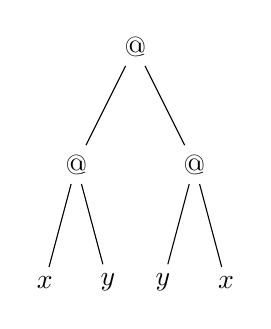
\begin{tikzpicture}
      [level 1/.style={sibling distance=15mm},
        level 2/.style={sibling distance=8mm}]
  \node at (0,0) {@}
  child { node {@}
      child {node {$x$}}
      child { node {$y$} }}
  child { node {@} 
      child {node {$y$}}
      child { node {$x$} }};
 \end{tikzpicture}

  \item

    \

    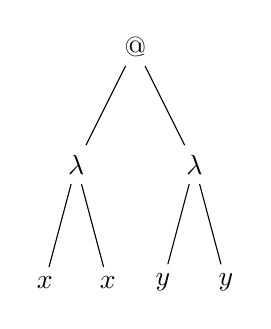
\begin{tikzpicture}
      [level 1/.style={sibling distance=15mm},
        level 2/.style={sibling distance=8mm}]
  \node at (0,0) {@}
  child { node {$\lambda$}
      child {node {$x$}}
      child { node {$x$} }}
  child { node {$\lambda$} 
      child {node {$y$}}
      child { node {$y$} }};
 \end{tikzpicture}


  \item

    \

    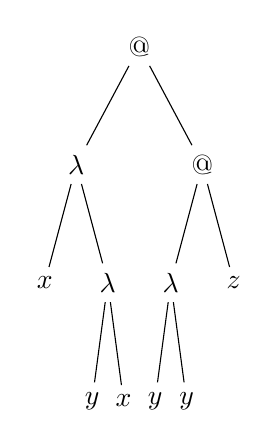
\begin{tikzpicture}
      [level 1/.style={sibling distance=16mm},
        level 2/.style={sibling distance=8mm},
          level 3/.style={sibling distance=4mm}]
  \node at (0,0) {@}
  child { node {$\lambda$}
      child {node {$x$}}
      child { node {$\lambda$}
        child {node {$y$}}
        child {node {$x$}}}}
  child { node {@}
    child { node {$\lambda$} 
        child {node {$y$}}
        child { node {$y$} }}
    child { node {$z$}}};
 \end{tikzpicture}



  \item

    \

    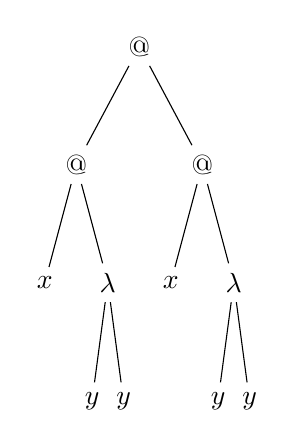
\begin{tikzpicture}
      [level 1/.style={sibling distance=16mm},
        level 2/.style={sibling distance=8mm},
          level 3/.style={sibling distance=4mm}]
  \node at (0,0) {@}
  child { node {@}
      child {node {$x$}}
      child { node {$\lambda$}
        child {node {$y$}}
        child {node {$y$}}}}
  child { node {@}
    child { node {$x$}}
    child { node {$\lambda$} 
        child {node {$y$}}
        child { node {$y$} }}};
 \end{tikzpicture}


  \end{enumerate}


  \end{enumerate}
  
\subsection{Kinds of variable occurrences}

 For each of the given terms, draw them in tree form and then
 indicate, in the same way as in Figure~\ref{fig:varocc}, which
 variable occurrences are binding (please underline), which are bound
 (please circle), and which are free (please box):
\begin{enumerate}

\item $y$

\vspace{.5cm}
\item $\lambda\, y.\ y$

\vspace{.5cm}
\item $(\lambda\, x.\, x\ x)\ y$

\vspace{.5cm}
\item $\lambda\, x.\, (\lambda\, y.\, x)\ y$

\vspace{.5cm}
\item $\lambda\, y.\, \lambda\, z.\, x\ y\ y\ (w\ z)$

\vspace{.5cm}
\end{enumerate}

\subsection{Capture-avoiding substitution}

For each of the following, write the result of the substitution or that it is undefined.

\begin{enumerate}
\item $[x/y]\lam{z}{y\ y}$
  
  \vspace{.5cm}

\item $[(x\ x)/y]\lam{z}{z\ (y\ y)}$

  \vspace{.5cm}

\item $[(x\ x)/y]\lam{y}{z\ y}$

  \vspace{.5cm}

\item $[\lam{x}{x}/y]\lam{z}{y\ \lam{y}{y\ z}}$

  \vspace{.5cm}

\item $[\lam{x}{y}/z]\lam{y}{y\ z}$
  \end{enumerate}


\subsection{Single-step $\beta$-reduction}

\begin{enumerate}
  \item Each of the following reductions is allowed by Definition~\ref{def:betactxt}.  For each reduction, indicate the instantiations of the meta-variables $x$, $t$, $t'$, and $t''$ of Definition~\ref{def:betactxt} (as in the examples in Section~\ref{sec:betaex}).
    \begin{enumerate}
    \item $\lam{x}{(\lam{y}{y})\ \lam{z}{z}}\ \betar \lam{x}{\lam{z}{z}}$
      \vspace{.5cm}
    \item $(\lam{y}{y})\ (z\ z)\ z\ \betar z\ z\ z$
      \vspace{.5cm}
    \item $z\ (\lam{y}{(\lam{z}{z\ z})\ (y\ y)}) \betar z\ \lam{y}{y\ y\ (y\ y)}$
      \vspace{.5cm}
    \item $(\lam{x}{\lam{y}{x\ x}})\ (z\ \lam{z}{z}) \betar \lam{y}{z\ (\lam{z}{z})\ (z\ \lam{z}{z})}$
      \vspace{.5cm}
    \item $(\lam{x}{\lam{y}{y}})\ z \betar \lam{y}{y}$
      \vspace{.5cm}
    \end{enumerate}

  \item Write derivations using the rules of Figure~\ref{fig:betar} for the $\beta$-reductions of parts (a), (b), (c) of the previous problem.

   \end{enumerate}

\subsection{$\alpha$-equivalence}

For each pair of terms, indicate whether or not they are $\alpha$-equivalent:
\begin{enumerate}
\item $\lam{x}{\lam{y}{y\ x}}$ and $\lam{x}{\lam{x}{y\ x}}$
  \vspace{.5cm}
\item $x\ \lam{y}{x}$ and $x\ \lam{w}{x}$
  \vspace{.5cm}
\item $x\ \lam{y}{x}$ and $y\ \lam{x}{y}$
  \vspace{.5cm}
\item $\lam{z}{(\lam{x}{x\ z})\ \lam{y}{z\ y}}$ and $\lam{q}{(\lam{y}{y\ q})\ \lam{y}{q\ y}}$
  \vspace{.5cm}
\end{enumerate}

\subsection{Multi-step $\beta$-reduction}

\begin{enumerate}

\item Write maximal $\curva$-reduction sequences starting with the given term.  Be careful with your renamings!

\begin{enumerate}
\item $\lam{y}{(\lam{x}{\lam{y}{x\ (x\ y)}})\ \lam{x}{y\ x}}$
  \vspace{.5cm}
\item $\lam{x}{\lam{y}{(\lam{z}{\lam{y}{\lam{x}{z\ z}}})\ \lam{z}{x\ y}}}$
  \vspace{.5cm}
\end{enumerate}

% answer: \delta app (in terms of Chapter 2)
\item Find an example of a term $t$ and number $n$ of $\beta$-steps where
  \begin{itemize}
  \item there exists a term $t'$ such that $t (=_\alpha\ \leadsto_\beta^n\ =_\alpha\ \leadsto_\beta) t'$, but
  \item there does not exist a term $t'$ such that $t (=_\alpha\ \leadsto_\beta^{n+1}) t'$.
  \end{itemize}
  \noindent In other words, this problem asks you to find an example of a term where a second $\alpha$-equivalence step is required in order to
  complete a sequence of $\beta$-reductions.  As a hint (because the problem is a bit tricky):
  \begin{itemize}
  \item If all bound and free variables are distinct from each other, then it is never necessary to rename to perform a single $\beta$-reduction, so it might seem like an initial $=_\alpha$-step would suffice to obviate any subsequent renamings... 
    \item ...but it is not! Ask yourself if there is a way that starting with a term where all bound and free variables are distinct from each other, one could arrive at a term that does not have that property; and then use this to construct a term where a second $=_\alpha$-step is required.

  \end{itemize}
\end{enumerate}

\chapter{Programming in Lambda Calculus}
\label{ch:prog}

\section{Basic functions}
\label{sec:basicfuncs}

Let us consider a few basic lambda terms that are useful for
programming in lambda calculus.  We will give names to the terms we
consider, as meta-linguistic abbreviations.  Let us use the syntax $N
:= t$ to indicate (in our meta-language) that we wish to use name $N$
as an abbreviation for term $t$.  In all cases, our choice of names
will be justified by the behavior of the term when applied to various
arguments.  By behavior, I mean the term's $\beta$-reductions.

\paradef{.5}{The identity function.} 
\[
\textit{id} := \lam{x}{x}
\]
\noindent This term really does behave like the mathematical
(set-theoretic, let us say) identity function, since if we apply
\textit{id} to anything, we just get back that same value.\index{identity \textit{id}}  We have

\[
\textit{id}\ t \ \ \betaa^* \ \ t
\]

\paradef{0}{Self-application operator.}
\[
\delta := \lam{x}{x\ x}
\]
\noindent This operator applies input $x$ to $x$. \index{self-application $\delta$}
We also have
\[
\Omega := \delta\ \delta
\]
\noindent This term has no normal form, reducing forever to itself:\index{diverging term $\Omega$}
\[
\begin{array}{ll}
  \underline{\delta}\ \delta & = \\
  \underline{(\lam{x}{x\ x})\ \delta} & \betaa \\
  \delta\ \delta &\
\end{array}
\]

\paradef{0}{Composition.}
\[
\textit{compose} := \lam{f}{\lam{g}{\lam{x}{f\ (g\ x)}}}
\]
\noindent This term can be applied to any terms $f$ and $g$, and it
will return a term that behaves like their composition: it applies $f$
after $g$ to its input $x$.  It is nice to borrow mathematical notation for
function composition and write $f \circ g$ for $\textit{compose}\ f\ g$.
Here are a few examples using \textit{compose}:\index{composition \textit{compose} (or $\circ$)}
\begin{itemize}
\item $\textit{id} \circ \textit{id} \ \ \betaa^*\ \ \textit{id}$
\item $\delta\circ \delta \ \ \betaa^*\ \ \lam{x}{x\ x\ (x\ x)}$:
\[
\begin{array}{ll}
  \underline{\delta\circ \delta} & = \\
  \underline{\textit{compose}}\ \delta\ \delta & = \\
  \underline{(\lam{f}{\lam{g}{\lam{x}{f\ (g\ x)}}})\ \delta}\ \delta & \betaa \\
  \underline{(\lam{g}{\lam{x}{\delta\ (g\ x)}})\ \delta} & \betaa \\
  \lam{x}{\delta\ (\delta\ x)} & \betaa \\
  \lam{x}{\delta\ \underline{(\delta\ x)}} & \betaa \\
  \lam{x}{\underline{\delta\ (x\ x)}} & \betaa \\
  \lam{x}{(x\ x)\ (x\ x)} & \ 
\end{array}
\]
  
\end{itemize}

\paradef{.5}{Application operator.}
\[
\textit{app} := \lam{x}{\lam{y}{x\ y}}
\]
\noindent This term takes in inputs $x$ and $y$ and returns the result of applying $x$ to $y$.  So it is a term which acts like the term construct of application.

\section{Representing numbers with the Church encoding}
\label{sec:churchenc}

For Church's original goal of a foundation for mathematics, it is
paramount that there is some way to represent natural numbers, and the
intuitively computable operations on them, as lambda terms.  Happily,
there are several such \emph{lambda encodings} for representing data
as lambda terms.  Here we see the first, which is Church's own encoding.\index{Church encoding}

Any lambda encoding must represent data as lambda terms implementing
some behavioral interface.  That is, data are defined by what they do,
not what they are.  The idea of the Church encoding more specifically
is to define numbers as their own iteration functions: functions which
take in another function $f$ and starting point $x$, and repeatedly
call $f$ starting with $x$.  Let us write $\rep{n}$ to mean the lambda
term representing $n\in\mathbb{N}$.  Then the Church encoding defines:

\[
\begin{array}{lll}
  \rep{n} & = & \lam{f}{\lam{x}{\underbrace{f \ (\cdots\  (f}_{n}\ x))}}
\end{array}
\]
\noindent So we have these concrete examples:

\[
\begin{array}{lll}
  0 & := & \lam{f}{\lam{x}{x}} \\
  1 & := & \lam{f}{\lam{x}{f\ x}} \\
  2 & := & \lam{f}{\lam{a}{f\ (f\ x)}} \\
  3 & := & \lam{f}{\lam{a}{f\ (f\ (f\ x))}} \\  
  \multicolumn{3}{l}{\cdots}
\end{array}
\]

\noindent In passing, we may observe that $1$ and $\textit{app}$ are $\alpha$-equivalent
terms.  When representing data as lambda terms, such coincidences
sometimes occur.

\section{Operations on Church-encoded natural numbers}

Let us see now how to define some basic operations on Church-encoded
natural numbers.

\paradef{.5}{Successor.} The mathematical successor
operation on $\mathbb{N}$ takes in $n$
and returns $n+1$ (i.e., the next number).  Here is the definition for
Church-encoded naturals:
\[
\textit{succ}\ :=\ \lam{n}{\lam{f}{\lam{x}{f\ (n\ f\ x)}}}
\]
\noindent To understand this, let us first see an example:
\[
\begin{array}{ll}
  \underline{\textit{succ}}\ 2 & = \\
  \underline{(\lam{n}{\lam{f}{\lam{x}{f\ (n\ f\ x)}}})\ 2} & \betaa \\
  \lam{f}{\lam{x}{f\ (\underline{2}\ f\ x)}} & = \\
  \lam{f}{\lam{x}{f\ (\underline{\lam{f}{(\lam{x}{f\ (f\ x)})}\ f}\ x)}} & \betaa \\
  \lam{f}{\lam{x}{f\ (\underline{(\lam{x}{f\ (f\ x)})\ x})}} & \betaa \\
  \lam{f}{\lam{x}{f\ (f\ (f\ x))}} & = \\
  3
\end{array}
\]
More generally, if $n\in\mathbb{N}$, then $\textit{succ}\ \rep{n}$ reduces to $\rep{n+1}$.

\paradef{.5}{Addition.}  To compute $\rep{m+n}$ from $\rep{m}$ and $\rep{n}$, the idea is similar to that for successor, except
that here we wish to add not just one $f$ to the left of $\underbrace{f \ \cdots\  (f }_{n}\ x)$, but $m$ applications of $f$.  For
then we would have $m+n$ applications of $f$ as desired for $\rep{m+n}$.  And fortunately, $\rep{m}$ itself gives us the power
to apply $f$ $m$ times to some starting value $Q$, by writing $m\ f\ Q$.  Here, we want $n\ f\ x$ for $Q$.  So the definition
of addition is:
\[
\textit{add} \ := \ \lam{m}{\lam{n}{\lam{f}{\lam{x}{m\ f\ (n\ f\ x)}}}}
\]

\paradef{0}{Predecessor.} Kleene was the first to crack the puzzle of how to compute the $\rep{n}$ from $\rep{n+1}$.
His definition is somewhat complicated, so here is a simpler one.  To my knowledge, this is original.  
\[
\begin{array}{lll}
\textit{just} & := & \lam{n}{\lam{j}{\lam{k}{j\ n}}} \\
\textit{pred} & := & \lam{n}{n\ (\lam{m}{\textit{just}\ (m\ \textit{succ}\ 0)})\ 0\ \textit{id}\ 0}
\end{array}
\]
\noindent Writing $F$ for $\lam{m}{\textit{just}\ (m\ \textit{succ}\ 0)}$, let us first see how $2\ F\ 0$ computes:
\[
\begin{array}{ll}
  \underline{2\ F}\ 0 & \betaa \\
  \underline{(\lam{a}{F\ (F\ a)})\ 0} & \betaa \\
  F\ (\underline{F\ 0}) & \betaa \\
  F\ (\textit{just}\ (\underline{0\ \textit{succ}}\ 0)) & \betaa \\
  F\ (\textit{just}\ (\underline{\lam{a}{a}\ 0})) & \betaa \\
  F\ (\underline{\textit{just}\ 0}) & \betaa \\
  \underline{F\ \lam{j}{\lam{k}{j\ 0}}} & \betaa \\    
  \textit{just}\ (\underline{(\lam{j}{\lam{k}{j\ 0}})\ \textit{succ}}\ 0) & \betaa \\
  \textit{just}\ (\underline{(\lam{k}{\textit{succ}\ 0})\ 0}) & \betaa \\
  \underline{\textit{just}\ (\textit{succ}\ 0)} & \betaa \\
  \lam{j}{\lam{k}{j\ (\textit{succ}\ 0)}} & \ 
\end{array}
\]
\noindent Now here is the reduction for $\textit{pred}\ 2$:
\[
\begin{array}{ll}
  \underline{\textit{pred}\ 2} & \betaa \\
  \underline{2\ F\ 0}\ \textit{id}\ 0 & \betaa^* \textnormal{[by above reduction sequence]}\\
  \underline{(\lam{j}{\lam{k}{j\ (\textit{succ}\ 0)}})\ \textit{id}}\ 0 & \betaa \\
  \underline{(\lam{k}{\textit{id}\ (\textit{succ}\ 0)})\ 0} & \betaa \\
  \underline{\textit{id}\ (\textit{succ}\ 0)} & \betaa \\
  \underline{\textit{succ}\ 0} & \betaa^* \\
  1 &\ 
\end{array}
\]
  

\paradef{0}{Another predecessor.}  Here is a different, trickier definition of predecessor, which one can find online (sadly, I do
not know who invented it):
\[
\textit{pred}\ :=\ \lam{n}{\lam{f}{\lam{x}{n\ (\lam{g}{\lam{h}{h\ (g\ f)}})\ (\lam{h}{x})\ \textit{id}}}}
\]
\noindent To understand how this works, let us write $F$ for $\lam{g}{\lam{h}{h\ (g\ f)}}$, and $A$ for $\lam{h}{x}$, and
see how $3\ F\ A$ computes:
\[
\begin{array}{ll}
  \underline{3\ F}\ A & \betaa \\
  (\lam{x}{F\ (F\ (F\ x))})\ A & \betaa \\
  F\ (F\ (\underline{F\ A})) & = \\
  F\ (F\ (\underline{(\lam{g}{\lam{h}{h\ (g\ f)}})\ \lam{h}{x}})) & \betaa \\  
  F\ (F\ (\lam{h}{h\ \underline{((\lam{h}{x})\ f)}})) & \betaa \\
  F\ (\underline{F}\ (\lam{h}{h\ x})) & = \\
  F\ (\underline{(\lam{g}{\lam{h}{h\ (g\ f)}})\ (\lam{h}{h\ x})}) & \betaa \\      
  F\ (\lam{h}{h\ \underline{((\lam{h}{h\ x})\ f)}}) & \betaa \\
  \underline{F}\ (\lam{h}{h\ (f\ x)}) & = \\
  \underline{(\lam{g}{\lam{h}{h\ (g\ f)}})\ (\lam{h}{h\ (f\ x)})} & \betaa \\
  \lam{h}{h\ \underline{((\lam{h}{h\ (f\ x)})\ f)}} & \betaa \\
  \lam{h}{h\ (f\ (f\ x))} & \
\end{array}
\]

What is happening here?  We see that $3\ F\ A$ has reduced to something similar to $f\ (f\ (f\ x))$, but
with a critical twist: we have $\lambda$-abstracted away the function for the first call to $f$, leaving
the other calls intact.  This gives us what we could think of as a ``flexible'' version of $f\ (f\ (f\ x))$, where we get
to choose which function to call instead of $f$ for the outer application.  And the definition of predecessor makes use of this flexibility
by applying the whole result to \textit{id}.  That produces, then, just $f\ (f\ x)$.  So, understanding $F$ and $A$ to be grafted
into the expression on the second line below (capturing their free variables $f$ and $x$), we have
\[
\begin{array}{ll}
  \textit{pred}\ 3 & \betaa^* \\
  \lam{f}{\lam{x}{\underline{3\ F\ A}\ \textit{id}}} & \betaa^* \\
  \lam{f}{\lam{x}{\underline{(\lam{h}{h\ (f\ (f\ x))})\ \textit{id}}}} & \betaa \\
  \lam{f}{\lam{x}{\underline{(\textit{id}\ (f\ (f\ x)))}}} & \betaa \\
  \lam{f}{\lam{x}{f\ (f\ x)}} & = \\  
  2 &\ 
\end{array}
\]

In some ways this is similar, as perhaps is inevitable, to the first
version of predecessor we saw: a value is computed from $\rep{n}$ that
is like $\rep{n}$ but allows calling another function -- in particular, \textit{id} -- instead of a
final successor.  In this second version of predecessor, that
value is computed underneath bindings of $f$ and $x$, so that
\textit{id} gets called on applications of $f$ to $x$.  In the
first version of predecessor, \textit{id} gets called on the entire
predecessor term, including bindings of $f$ and $x$.

\section{Representing booleans}
\label{sec:bool}

A simpler datatype than that of the natural numbers is the boolean
type, with values \textit{true} and \textit{false}.  The Church
encoding of this type is
\[
\begin{array}{lll}
  \textit{true} & := & \lam{x}{\lam{y}{x}} \\
  \textit{false} & := & \lam{x}{\lam{y}{y}}
\end{array}
\]
\noindent Each boolean accepts two inputs (one at a time), and returns
one of these.  \textit{true} returns the first, while \textit{false}
returns the second.  Based on this idea, it is easy to see how to define
various boolean operations:
\[
\begin{array}{lll}
  \textit{not} & := & \lam{x}{x\ \textit{false}\ \textit{true}} \\
  \textit{and} & := & \lam{x}{\lam{y}{x\ y\ \textit{false}}}
\end{array}
\]
\noindent We negate (with \textit{not}) a boolean by applying it to
\textit{false} and then \textit{true}.  If the boolean itself is
\textit{true}, then it will return the first of these two inputs,
namely \textit{false}; if it is \textit{false}, it will return
\textit{true}.  This is the desired behavior.  Similarly, \textit{and}
takes in inputs \textit{x} and \textit{y}.  It returns the result of
applying \textit{x} to \textit{y} and then \textit{false}.  If
\textit{x} is \textit{true}, then the result will be \textit{y}; and
this is what we would like for conjunction, since if the first boolean
(\textit{x}) is true, the conjunction's value coincides with the value
of the second (\textit{y}): true if \textit{y} is true, and false if
\textit{y} is false.  And if \textit{x} is \textit{false}, then the
second input (out of \textit{y} and \textit{false}) will be chosen; again,
the desired behavior, since this means conjoining \textit{false} with
anything will reduce to \textit{false}.

It is worth emphasizing that applying boolean operations to values
that are not booleans does not result in an error as it might
in some programming languages.  Here, every lambda term has a well-defined
behavior in the form of its $\beta$-reductions.  But the results of
applications violating the intuitive typings we have in mind for
these operations may be somewhat inscrutable.

\section{Ordered pairs}

It is often convenient to program with a representation of ordered pairs $(x,y)$, given representations of $x$ and $y$.
To construct the representation of a pair, we use this function:
\[
\textit{pair} \ :=\ \lam{x}{\lam{y}{\lam{c}{c\ x\ y}}}
\]
\noindent The idea is that given the components $x$ and $y$ of the
pair, we represent (by the \textit{pair} function) the pair itself as
$\lam{c}{c\ x\ y}$.  This definition embodies the idea that a pair of
$x$ and $y$ is something that can make $x$ and $y$ available for
subsequent computation.  This is done in the encoding by applying the
pair to a function which is expecting the components.

For example, we may define \textit{fst} (``first'') and \textit{snd}
(``second''; these names are often used for these operations in
functional programming languages) as follows:
\[
\begin{array}{lll}
  \textit{fst} & := & \lam{p}{p\ \textit{true}} \\
  \textit{snd} & := & \lam{p}{p\ \textit{false}}
\end{array}
\]
\noindent Since \textit{true} returns the first of two arguments, and
\textit{false} the second, they are used to select either the first or
the second component, respectively, when passed as an argument to the
pair.  (As usual, these functions assume input \textit{p} is a pair
of the form $\lam{c}{c\ x\ y}$, and may give unexpected results
if applied to terms not of that form.)

\section{Representing numbers with the Scott encoding}

In Section~\ref{sec:churchenc}, we saw an elegant representation of
numbers as lambda terms, called the Church encoding.  Every number $n$
is represented as the $n$-fold composition operator.  While many
functions are concisely definable this way, the predecessor operation
required quite some ingenuity, and is asymptotically less efficient
than we might reasonably expect (taking time linear in $n$, instead of
constant time).  In this section, we consider an alternative lambda
encoding due to Dana Scott, which has a straightforward constant-time
predecessor.  With the Scott encoding, each number can be thought of
as a function $t$ that informs the caller whether $t$ represents a
successor number or zero.  In the former case, it also provides the
caller with the representation of the predecessor. The definition is:
\[
\begin{array}{lll}
  0 & := & \lam{f}{\lam{x}{x}} \\
  1 & := & \lam{f}{\lam{x}{f\ 0}} \\
  2 & := & \lam{f}{\lam{x}{f\ 1}} \\
  \multicolumn{3}{l}{\cdots} \\
  \rep{n+1} & := & \lam{f}{\lam{x}{f\ \rep{n}}} \\
  \multicolumn{3}{l}{\cdots} 
\end{array}
\]
So every $\rep{n}$ accepts two inputs $f$ and $x$, and if
$n$ is $0$, returns $x$; and if $n$ is $m+1$ for some $m$, returns
$f\ \rep{m}$.  This makes available the predecessor $\rep{m}$, and
thus the actual predecessor function is easily defined:
\[
\textit{pred} \ := \ \lam{n}{n\ \textit{id}\ 0}
\]
\noindent Here, \textit{id} is passed for $f$ and $0$ for $x$.  This means
that for any Scott-encoded successor number, we have the following reduction:
\[
\begin{array}{ll}
  \underline{\textit{pred}}\ \rep{n+1} & = \\
\underline{(\lam{n}{n\ \textit{id}\ 0})\ \rep{n+1}} & \betaa \\
\underline{\rep{n+1}}\ \textit{id}\ 0 & = \\
\underline{(\lam{f}{\lam{x}{f\ \rep{n}}})\ \textit{id}}\ 0 & \betaa \\
\underline{(\lam{x}{\textit{id}\ \rep{n}})\ 0} & \betaa \\
\underline{\textit{id}\ \rep{n}} & \betaa \\
\rep{n} & \
\end{array}
\]
\noindent And this is the desired result: $\textit{pred}\ \rep{n+1}
\betaa^* \rep{n}$.  Furthermore, we can see that this reduction required
four steps of $\beta$-reduction, independent of the value of $n$.
This is in contrast to the case with the Church encoding, where the
number of steps was proportional to $n$.

It is obvious from the encoding that the successor function \textit{succ} for Scott-encoded numbers should be:
\[
\textit{succ}\ := \ \lam{n}{\lam{f}{\lam{x}{f n}}}
\]

\section{The Y combinator}
\label{sec:y}

While it is very straightforward to define predecessor on
Scott-encoded numbers, other operations pose a problem.  The Church
encoding takes $n$-fold iteration as the representation of $n$, and
hence has no difficulty defining iterative functions.  Not so the
Scott encoding, and indeed, the only natural way to recurse is to
avail ourselves of a term implementing \emph{general recursion} (this
is recursion that may fail to terminate).  (It should be noted that
there is an extremely tricky way to derive iteration for Scott encodings, but
we will not consider this here~\cite{lepigre+19}.)

General recursion in lambda calculus is provided using a term traditionally
denoted $Y$:
\[
Y \ :=\ \lam{f}{(\lam{x}{f\ (x\ x)})\ (\lam{x}{f\ (x\ x)})}
\]
\noindent This term is usually called a \emph{combinator}, which is an
informal notion indicating that a lambda term is of interest primarily
for use as a building block for defining other functions (as opposed,
say, to implementing some particular algorithm valuable in its own
right).\index{combinator}\index{Y combinator} In this sense, some other terms we have
encountered so far, like identity and composition functions
(\textit{compose}, \textit{id} of Section~\ref{sec:basicfuncs}), are
also reasonably considered combinators.

Terminology aside, let us see how the $Y$ combinator works and how we
can use it to define operations on Scott-encoded numbers.  Suppose $t$ is any
lambda term not containing $x$ free.  Then we have:
\[
\begin{array}{ll}
  \underline{Y}\ t & = \\
  \underline{(\lam{f}{(\lam{x}{f\ (x\ x)})\ (\lam{x}{f\ (x\ x)})})\ t} & \betaa \\
  \underline{(\lam{x}{t\ (x\ x)})\ (\lam{x}{t\ (x\ x)})} & \betaa \\
  t\ \underline{((\lam{x}{t\ (x\ x)})\ (\lam{x}{t\ (x\ x)}))} & =_\beta \\
  t\ (Y\ t)
\end{array}
\]
\noindent So we see that $Y\ t$ is $\beta$-equivalent to $t\ (Y\ t)$.  This fact is so important that
it is worth highlighting as an equation:
\[
Y\ t\ =_\beta \ t\ (Y\ t)
\]
\noindent Swapping sides will shortly be revealing:
\[
t\ (Y\ t)\ =_\beta \ Y\ t
\]
\noindent This matches the form of a fixed-point equation for $t$.  In mathematics, a fixed point of a function $F$ is an input $X$ such that
\[
F(X) = X
\]
\noindent Here, with application of lambda terms playing the role of function invocation, and $\beta$-equivalence taking the place of equality,
we can write this as:
\[
F\ X =_\beta X
\]
\noindent For term $t$, this becomes
\[
t\ X =_\beta X
\]
\noindent And indeed, the equation we derived above is of this form, with $Y\ t$ for $X$.

Now what is the significance of this?  It shows us that, contrary to
what we usually find in mathematics, in lambda calculus every function
has a fixed point.  How peculiar!  Certainly some mathematical
functions have fixed points.  Take (mathematical) predecessor on
natural numbers, with the assumption that \textit{pred} of $0$ is $0$.
Then $0$ is a fixed point of \textit{pred}.  But consider boolean negation.
There is no boolean $b$ such that $\textit{not}\ b$ equals $b$ (neither possible
value for $b$, namely \textit{true} or \textit{false}, works).  Strangely, though,
in lambda calculus, we have just seen the general equation of $t\ (Y\ t)$ and $Y\ t$.
This means that
\[
\textit{not}\ (Y\ \textit{not}) =_\beta Y\ \textit{not}
\]
\noindent Something unusual is going on, and indeed, as we will see when we
turn to denotational semantics of lambda calculus, interpreting lambda calculus
in set theory requires significant ingenuity.

But to remain at the linguistic level for the moment, let us try to get an intuition
for how every term $t$ can have $Y\ t$ for a fixed point.  Let us write $U$ for $\lam{x}{t\ (x\ x)}$.  We have seen that
\[
\begin{array}{ll}
  \underline{Y\ t} & \betaa \\
  \underline{U\ U} & \betaa \\
  t\ (U\ U)&\ 
\end{array}
  \]
\noindent  This reduction sequence may then be continued as long as we wish:
\[
\begin{array}{ll}
  t\ \underline{(U\ U)}&\betaa \\
  t\ (t\ \underline{(U\ U)})&\betaa \\  
  t\ (t\ (t\ \underline{(U\ U)}))&\betaa \\
  \multicolumn{2}{l}{\cdots}
\end{array}
\]
\noindent If we had some notion of infinite lambda term, we might identify the limit of this infinite reduction sequence,
as this infinite right-nested application of $t$:
\[
t\ (t\ (t\ \cdots
\]
\noindent One can indeed develop an infinitary lambda calculus
allowing infinitary terms like this~\cite{kennaway1997}; but this is
beyond the scope of the book.  But with an infinitary term like
this as an informal guiding intuition, we can see how the fixed-point equation
makes sense.  $Y\ t$ denotes (informally) an infinite
right-nested application of $t$.  Applying $t$ one more time to this
does not change the infinite application, as it is still infinite!

Note that $U\ U$ is a lot like $\delta\ \delta$:
\[
\begin{array}{lll}
  U\ U & = & (\lam{x}{t\ (x\ x)})\ \lam{x}{t\ (x\ x)} \\
  \delta\ \delta & = & (\lam{x}{x\ x})\ \lam{x}{x\ x}
\end{array}
\]
\noindent We have just inserted $t$, but otherwise retain the central idea of self-application
for divergence.

How is this esoterically explained construction useful for programming?  Contrast
the situation with iteration using Church-encoded numbers.  There, $\rep{n}$ gives us the
power to repeat a function $n$ times:
\[
\underbrace{t\ \cdots\ (t}_n\ x)
\]
\noindent But what if we need to repeat a function more times than
just $n$ times?  We could imagine somehow increasing how many times
the composition is iterated, to some bigger number $n'$.  But the most
computationally powerful option is to extend the $n$-fold iteration of
$t$ to an infinite iteration of $t$:
\[
t\ (t\ (t\ \cdots
\]
\noindent But this is just what (informally) $Y\ t$ gives us!  So we
are using the power of diverging computation which we get through
self-application, to allow ourselves as many iterations of $t$ as we
could possibly need.  Fundamental results of recursion theory then
imply that we will of necessity need to accept the possibility of
divergence: we have given ourselves the ability to apply $t$ as many
times as we wish, and we cannot rule out the possibility that it gets
applied infinitely many times with no normal form reachable.

But there is still a puzzle.  How can we ever reach any normal form when
$Y\ t$ has an infinite reduction sequence?  The answer is that existence
of a single infinite reduction sequence does not mean all reduction
sequences are infinite.  Indeed, for a very simple example, consider
\[
(\lam{x}{\lam{y}{y}})\ \Omega
\]
\noindent This term has both an infinite reduction sequence, and also infinitely many finite reduction sequences.  For examples of the first and second, in order, consider:
\[
\begin{array}{l}
  (\lam{x}{\lam{y}{y}})\ \underline{\Omega}\ \betaa\ (\lam{x}{\lam{y}{y}})\ \underline{\Omega}\ \betaa \ \cdots \\
  \underline{(\lam{x}{\lam{y}{y}})\ \Omega} \ \betaa \ \lam{y}{y}
\end{array}
\]
\noindent The normalizing reduction sequence (the second one) drops out the non-normalizing $\Omega$ subterm.
Similarly, in our infinitary term
\[
t\ (t\ (t\ \cdots
\]
\noindent it could happen that there is a reduction to a normal form where an application of $t$ ends up dropping
its argument.  We will see an example next.

\section{Recursive operations on Scott-encoded numbers}

Let us define addition on Scott-encoded numbers using the $Y$ combinator.  The idea is that we wish to implement the following
system of recursive equations, using $Y$ to implement the recursion:
\[
\begin{array}{lll}
  \textit{add}\ 0\ m & = & m \\
  \textit{add}\ (\textit{succ}\ p)\ m & = & \textit{succ}\ (\fbox{\textit{add}}\ p\ m)
\end{array}
\]
\noindent Since the Scott-encoding gives us a way to distinguish whether a number is $0$ or a successor number, we can
easily choose whether between these equations based on the first input.  We then need to use $Y$ to implement the framed
recursion on the right-hand side of the second equation.  The definition is, the following, using helper definition \textit{addh} for
easier consideration below:
\[
\begin{array}{lll}
  \textit{addh} & := & \lam{\textit{add}}{\lam{n}{\lam{m}{n\ (\lam{p}{\textit{succ}\ (\textit{add}\ p\ m)})\ m}}} \\
  \textit{add} & := & Y\ \textit{addh}
  \end{array}
\]
\noindent Let us see how this works with an example, writing $U$ for $\lam{x}{\textit{addh}\ (x\ x)}$:
\[
\begin{array}{ll}
  \underline{\textit{add}}\ 2\ 2 & = \\
  \underline{Y\ \textit{addh}}\ 2\ 2 & \betaa \\
  \underline{U\ U}\ 2\ 2 & \betaa \\  
  \underline{\textit{addh}}\ (U\ U)\ 2\ 2 & = \\
  \underline{(\lam{\textit{add}}{\lam{n}{\lam{m}{n\ (\lam{p}{\textit{succ}\ (\textit{add}\ p\ m)})\ m}}})\ (U\ U)}\ 2\ 2 & \betaa \\  
  \underline{(\lam{n}{\lam{m}{n\ (\lam{p}{\textit{succ}\ (U\ U\ p\ m)})\ m}})\ 2\ 2} & \betaa^2 \\
  \underline{2}\ (\lam{p}{\textit{succ}\ (U\ U\ p\ 2)})\ 2 & = \\
  \underline{(\lam{f}{\lam{x}{f\ 1}})\ (\lam{p}{\textit{succ}\ (U\ U\ p\ 2)})\ 2} & \betaa^2 \\
  \underline{(\lam{p}{\textit{succ}\ (U\ U\ p\ 2)})\ 1} & \betaa \\
  \textit{succ}\ \underline{(U\ U\ 1\ 2)}) & \betaa^* \\
  \textit{succ}\ (\textit{succ}\ \underline{(U\ U\ 0\ 2)}) & \betaa^* \\
  \textit{succ}\ (\textit{succ}\ 2) & \betaa^* \\
  4 &\ 
  \end{array}
\]
\noindent We see in detail that $U\ U\ \rep{n+1}\ m$ reduces to
$\textit{succ}\ (U\ U\ \rep{n}\ m)$.  So we peel successors off the
first argument until we reach $0$, and then we return the second
argument (i.e., $m$).

\section{A direct approach to recursion on Scott-encoded numbers}

Instead of using the $Y$ combinator, it is possible to recurse
directly on Scott-encoded numbers.  A Scott-encoded number takes in a
function $f$ to call with the predecessor if the number is non-zero,
and a value $x$ to return if the number is zero.  The key idea,
attributed by Lepigre and Rafalli to Michel Parigot, is to have $f$
and $x$ themselves expect to be called with $f$ and $x$
again~\cite{lepigre:rafalli19}.  This enables in particular $f$ to
recurse.

Here is a definition of addition for the Scott encoding,
using this idea. I have abstracted out $f$ and $x$ for this
case, to help make clear where there is a self-application
happening.  The base case $x$ depends, in the definition of addition,
on the second addend, so we need to write $x\ m$ in the definition
of \textit{add}, instead of just $x$.
\begin{eqnarray*}
f & := & \lam{p}{\lam{s}{\lam{z}{\textit{succ}\ (p\ s\ z\ s\ z)}}} \\
x & := & \ \lam{m}{\lam{s}{\lam{z}{m}}} \\
\textit{add} & := & \lam{n}{\lam{m}{n\ f\ (x\ m)\ f\ (x\ m)}}
\end{eqnarray*}

\noindent Let us see this definition in action:

\[
\begin{array}{ll}
  \underline{\textit{add}\ 2\ 2} & \betaa^2 \\
  \underline{2\ f}\ (x\ 2)\ f\ (x\ 2) & \betaa \\
  \underline{f\ 1\ f\ (x\ 2)} & \betaa^3 \\
  \textit{succ}\ \underline{(1\ f\ (x\ 2)\ f\ (x\ 2))} & \betaa^4 \\
  \textit{succ}\ (\textit{succ}\ \underline{(0\ f\ (x\ 2)\ f\ (x\ 2))}) & \betaa \\
  \textit{succ}\ (\textit{succ}\ \underline{((x\ 2)\ f\ (x\ 2))}) & \betaa^3 \\
  \underline{\textit{succ}\ (\textit{succ}\ 2)} & \betaa^* \\    
  4
\end{array}
  \]

\section{The Parigot encoding}

Before (it seems) his discovery of a way to recurse on Scott-encoded
numbers, Parigot proposed an encoding that combines the Church and
Scott encodings:

\[
\begin{array}{lll}
  0 & := & \lam{f}{\lam{x}{x}} \\
  1 & := & \lam{f}{\lam{x}{f\ 0\ x}} \\
  2 & := & \lam{f}{\lam{x}{f\ 1\ (f\ 0\ x)}} \\
  3 & := & \lam{f}{\lam{x}{f\ 2\ (f\ 1\ (f\ 0\ x))}} \\
  \multicolumn{3}{l}{\cdots} \\
  \rep{n+2} & := & \lam{f}{\lam{x}{f\ \rep{n+1}\ (f\ \rep{n}\ (\cdots\ (f\ 0\ x)))}} \\
  \multicolumn{3}{l}{\cdots} 
\end{array}
\]

\noindent Another way to see the encoding is to observe that for every $n$,
\[
\rep{n+1}\ \betaeq\ \lam{f}{\lam{x}{f\ \rep{n}\ (\rep{n}\ f\ x)}}
\]
\noindent where $\betaeq$ denotes $\beta$-equivalence (Definition~\ref{def:betaeq})

\section{Exercises}

\subsection{$\beta$-reductions for some simple terms}

\begin{enumerate}
\item For each of the following terms, write down a $\beta$-normal form to which the term reduces.  You do not need to write out all the steps in a $\beta$-reduction sequence.  Please just give a $\beta$-normal form.

  \begin{enumerate}
  \item $\textit{app}\ \circ\ \textit{id}$
\vspace{.5cm}
  \item $\textit{app}\ \circ\ \textit{app}$
\vspace{.5cm}
  \item $\lam{z}{2\ z}$
\vspace{.5cm}
  \item $\delta\ \textit{app}$
\vspace{.5cm}
  \item $2\ 2$
\vspace{.5cm}
  \item $\textit{not}\ 2$ (as noted above, terms like this which violate intuitive typings do have a
    well-defined behavior)
\vspace{.5cm}
  \item $\textit{and}\ 1$
  \end{enumerate}

\item Please write out a maximal $\beta$-reduction sequence (renaming is not necessary, so we can use just $\betar$
  instead of $\betaa$) starting with $\textit{pred}\ 2$.

\end{enumerate}

\subsection{Programming in lambda calculus}

\begin{enumerate}
\item Define a disjunction operator (i.e., boolean ``or'') on Church-encoded booleans, and demonstrate that it is working by writing a maximal $\betaa$-reduction sequence starting with $\textit{or}\ \textit{false}\ \textit{true}$.

\item \ \textbf{[Challenge]} Find an alternative definition of \textit{pred} with similar form as above, namely
  \[
  \lam{n}{\lam{f}{\lam{x}{n\ F'\ A'\ t_1 \cdots t_k}}}
  \]
  \noindent for some terms $F'$ and $A'$ grafted into this expression (which hence might have free occurrences of $f$ or $x$ that get bound by the $\lambda$-abstractions of those two variables), and some extra terms $t_1, \cdots, t_k$.
  The critical requirement is that where $\rep{n+1}\ F\ A$ reduces (with the definition of $F$ and $A$ in the text) to $\lam{h}{h\ (\underbrace{f \cdots (f}_n\ x))}$, your version with your $F'$ and $A'$ and some of your extra terms should
  reduce to $\lam{h}{\underbrace{f \cdots (f}_n\ (h\ x))}$.

\item Define a function \textit{flip} which reverses the order of components in a pair.

\item Define a subtraction operation on Scott-encoded numbers.  Your term is free to invoke \textit{pred} for predecessor,
  and the $Y$ combinator (and other terms we have defined so far, if you wish).

  \item The term $Y\ Y$ has many different (infinite) reductions.  Try
    to indicate a little of the complexity of this term by showing
    prefixes of some of its reduction sequences.  It would be
    interesting to organize these initial parts of reduction sequences
    into a tree, so we can see how reduction can branch out in different
    ways from the starting point of $Y\ Y$.  (This problem is not concerned
    with giving an exact correct answer, but rather with showing that you
    have explored the reduction behavior of this rather exotic term.)
\end{enumerate}

\chapter{Confluence}

In this chapter, we prove a basic property of the lambda calculus,
called confluence.\index{confluence} Given a binary relation $\to$ on
a set $A$, an element $a \in A$ is confluent iff no matter which pair
of $\to$-paths we follow from $a$, ending in some elements $b$ and
$c$, there is a pair of $\to$-paths from $b$ and $c$ ending in a
common element $d$.  This can be expressed pictorially as:

\begin{center}
\begin{tikzpicture}
  \node at (0,2) (a){a};
  \node at (-2,0) (b){b};
  \node at (2,0) (c){c};
  \node at (0,-2) (d){d};

  \node at (.4,-1.85) {$*$};
  \node at (-.4,-1.85) {$*$};
  \node at (-1.85,.4) {$*$};
  \node at (1.85,.4) {$*$};

  \draw[->] (a) -- (b);
  \draw[->] (a) -- (c);
  \draw[->,dashed] (b) -- (d);
  \draw[->,dashed] (c) -- (d);  
\end{tikzpicture}
\end{center}

Confluence can be seen as a generalization of determinism
(Definition~\ref{def:det}, the property that whenever $a \to b$ and $a
\to c$, we have $b = c$).  For it might happen that we have paths from
$a$ that can reach distinct elements $b$ and $c$ (that is, $a \to^* b$
and $a \to^* c$, with $b \neq c$), but these elements can be joined
back at some element $d$ (so $b \to^*d$ and $c\to^*d$).  So $a$ is
nondeterministic, yet in a somewhat controlled way: no matter
which two paths we follow from $a$, there is always some way to
reconverge.

In this chapter, we will prove that the relation $\curva_\alpha \cup
\curva_\beta$ is confluent.  This relation subsumes the relation
$\betaa$ of single-step $\beta$-reduction with renaming
(Definition~\ref{def:betaa}), because it allows any sequence of
$\curva_\alpha$ and $\curva_\beta$ steps, while a non-trivial
$\betaa$-reduction sequence must end with a $\curva_\beta$ step.
Working with the more permissive relation will enable a cleaner
formulation of confluence.  The proof we will follow is attributed to
William Tait and Per Martin-L\"of (but never published by either of
them).  Some of our discussion is quite generic, however, and applies
to any binary relation $\to$ over some set of elements (not
necessarily terms).

We will use the notation $\abeta$ for the relation that we
will study in this chapter:

\begin{definition}
  \label{def:abeta}
  $\abeta$ is defined to be $\curva_\alpha \cup \curva_\beta$.
  \end{definition}

\section{The diamond property}

A property quite similar to confluence of a relation $\to$ is
the following:
\begin{definition}[Diamond property]
  An element $x$ has the diamond property with respect to relation
  $\to$ on set $A$ iff $x \to y$ and $x \to z$ imply that there exists an element $q$
  with $y \to q$ and $z \to q$. The relation $\to$ itself has the diamond
  property, denoted $\textit{Diamond}(\to)$, iff every element of $A$ has
  the diamond property with respect to $\to$.  \index{diamond property}
  \end{definition}
\noindent Pictorially, this is very similar to the diagram for confluence,
but without the stars:

\begin{center}
\begin{tikzpicture}
  \node at (0,1.75) (a){a};
  \node at (-1.75,0) (b){b};
  \node at (1.75,0) (c){c};
  \node at (0,-1.75) (d){d};


  \draw[->] (a) -- (b);
  \draw[->] (a) -- (c);
  \draw[->,dashed] (b) -- (d);
  \draw[->,dashed] (c) -- (d);  
\end{tikzpicture}
\end{center}

Indeed, an alternative definition of confluence of $\to$ is simply to say that $\to^*$ has the diamond property.
In this form, the following lemma states that reflexive-transitive closure preserves the diamond property:
\begin{theorem}[Star preserves diamond]
\label{thm:stardia}
  $\textit{Diamond}(\to)$ implies $\textit{Diamond}(\to^*)$
\end{theorem}
\begin{proof}
  Assume $\textit{Diamond}(\to)$ and $x$, $y$, $z$ with $x \to^*y$ and $x \to^* z$.  We proceed
  by induction on the derivation of $x \to^* y$ (recall the three rules defining the reflexive-transitive
  closure, in Figure~\ref{fig:rtcl}):

  \case{ }
  \[
  \infer{x \to^* y}{x \to y}
  \]
  \noindent Here we will proceed by an inner induction on the derivation of $x \to^* z$ to show that there
  is a $q$ with $y\to^*q$ and $z \to q$, for all $x$, $y$, and $z$ with $x\to y$.

  \case{ (inner)}
  \[
  \infer{x \to^* z}{x \to z}
  \]
  \noindent We have exactly the assumptions of the diamond property, so we can conclude that there is a $q$
  with $y \to q$ and $z \to q$.  Our inner induction requires us to show $y \to^* q$, which follows from
  this same inclusion rule whose inferences we are presently considering.

  \case{ (inner)}
  \[
  \infer{x \to^* x}{\ }
  \]
  \noindent We have learned in this case that $x = z$, since that is the only way the reflexivity
  rule could be applied to prove $x \to^*z$.  
  For whatever $q$ we select, we must prove $y \to^*q$ and $z \to q$.  
  Since $x = z$, it suffices to show $y \to^*q$ and $x \to q$.  Let us take $q$ to be $y$.
  So we must show $y \to^* y$, which follows by the reflexivity rule; and $x \to y$, which
  follows by assumption in this inner induction.

  \case{ (inner)}
  \[
  \infer{x \to^* z}{x \to^*w & w \to^* z}
  \]
  \noindent We may apply the induction hypothesis to the first premise of this
  inference.  So the $x$, $y$, and $z$ of the induction hypothesis are instantiated
  with $x$, $y$, and $w$, respectively.  The induction hypothesis then tells us that
  there is an element $q$ such that $y \to^*q$ and $w \to q$.  We may now apply the
  induction hypothesis to the second premise, where we
  instantiate $x$, $y$, and $z$ with $w$, $q$, and $z$, respectively.  This tells
  us that there is a $q'$ with $q\to^*q'$ and $z \to q'$.  Combining a couple of
  the facts we have so far (namely, $y\to^* q$ and $q\to^* q'$) using the
  transitivity rule gives us $y \to^* q'$.  And we have $z \to q'$.
  So we may take the element $q$ which we are supposed to identify, to be this $q'$.
  This concludes the inner induction.  Note that this induction could be (and often is)
  broken out as a separate lemma, since it does not need to invoke the outer induction
  hypothesis.
  
  We may now return to our outer induction:

  \case{ }
  \[
  \infer{x \to^* x}{\ }
  \]
  \noindent In this case, we have learned that $x = y$, since that is the only way a reflexivity
  inference could prove $x \to^* y$.  Our goal is to identify an element $q$ with $y \to^* q$ and $z \to^* q$,
  but since $x = y$, it suffices to find a $q$ with $x \to^* q$ and $z \to^* q$.  Take $q$ to be $z$, and
  we have $x \to^* z$ by assumption of this induction, and $z \to^* z$ by reflexivity.

  \case{ }
  \[
  \infer{x \to^* y}{x \to^* w & w \to^* y}
  \]
  \noindent By the induction hypothesis applied to the first premise, there is a $q$ with
  $w \to^* q$ and $z \to^* q$.  We may now apply the induction hypothesis to the second
  premise, instantiating $x$, $y$, and $z$ with $w$, $y$, and $q$, respectively.  This
  produces a $q'$ with $y\to^* q'$ and $q\to^* q'$.  Let us take $q'$ to be the $q$ required
  by the theorem.  Since $z\to^*q$ and $q\to^* q'$, we have $z \to^* q'$ by transitivity;
  and $y\to^* q'$ was already concluded.
  

  \end{proof}

Thanks to Theorem~\ref{thm:stardia}, we know that if we would like to establish confluence of $\abeta$, it
would suffice to prove that this relation has the diamond property.  But this is easily seen
not to be the case.  Consider the diagram in Figure~\ref{fig:betanodia}.  The term at the peak (top) of the diagram
has two redexes, shown underlined.  Down the left side of the peak we reduce the leftmost redex, and down the right
side, the rightmost.  We can indeed join the resulting terms, at term $z\ z$, but this requires two steps along the
left side of the valley (running diagonally right to $z\ z$), while needing just one step along the right
side of the valley.  This example shows:

\begin{theorem}
  $\abeta$ lacks the diamond property
\end{theorem}

It is the beautiful observation at the heart of the Tait--Martin-L\"of proof of confluence that
while $\beta$-reduction lacks the diamond property, still another relation $\Pred^\alpha$ can be defined which
satisfies the diamond property, and where $(\Pred^\alpha)^* = \betaa^*$.  This will lead us to our goal,
thanks to the following theorem:
\begin{theorem}
  \label{thm:tml}
  Let $S$ be a relation on a set $A$, and suppose that there is a relation $R$ on $A$ such that
  $\textit{Diamond}(R)$ and $R^* = S^*$.  Then $S$ is confluent.
\end{theorem}

\begin{proof}
  Confluence
  of $S$, is equivalent to $\textit{Diamond}(S^*)$.  Since $R^* = S^*$ by assumption, it suffices
  then to prove $\textit{Diamond}(R^*)$.  By Theorem~\ref{thm:stardia}, this follows
  from $\textit{Diamond}(R)$, which we have by assumption.
\end{proof}

Actually, the task of confluence is made even easier by observing the following:
\begin{lemma}
  If $S \subseteq R \subseteq S^*$, then $R^* = S^*$.
\end{lemma}
\begin{proof}
  By monotonicity of the reflexive-transitive closure operator (Lemma~\ref{lem:starmono}),
  $S \subseteq R$ implies $S^* \subseteq R^*$.  So we have inclusions both directions
  between $S^*$ and $R^*$, implying (in set theory) that they are equal.
  \end{proof}

\noindent So to use Theorem~\ref{thm:tml}, by this lemma, we just need to identify some relation
intermediate between $\abeta$ and $\abeta^*$, which satisfies the diamond property.  This relation
is $\Pred^\alpha$, defined next.

\begin{figure}

  \begin{center}
    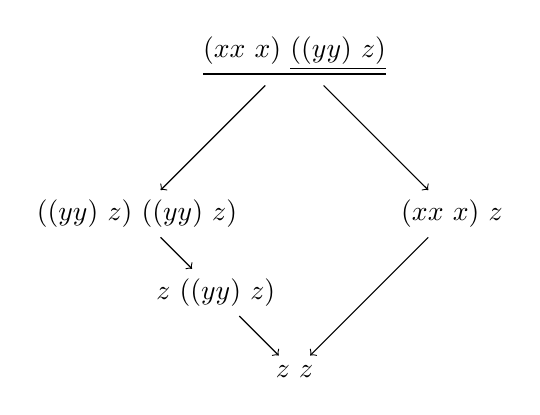
\begin{tikzpicture}
      \node at (0,2)(a){$\underline{(\lam{x}{x\ x})\ \underline{((\lam{y}{y})\ z)}}$};
      \node at (-2,0)(b){$((\lam{y}{y})\ z)\ ((\lam{y}{y})\ z)$};
      \node at (-1,-1)(c){$z\ ((\lam{y}{y})\ z)$};
      \node at (2,0)(d){$(\lam{x}{x\ x})\ z$};
      \node at (0,-2)(e){$z\ z$};

      \draw[->] (a) -- (b);
      \draw[->] (b) -- (c);
      \draw[->] (c) -- (e);
      \draw[->] (a) -- (d);
      \draw[->] (d) -- (e);
      \end{tikzpicture}
    \end{center}

\caption{Counterexample showing that $\beta$-reduction lacks the diamond property.}
\label{fig:betanodia}

\end{figure}

\section{Parallel reduction}

In this section, we define a relation $\Pred^\alpha$ for parallel reduction with renaming\index{parallel reduction}\index{$\Pred^\alpha$}.  This relation will be the desired
intermediate relation between $\abeta$ and $\abeta^*$, with the diamond property.  $\Pred$ is defined
by the rules of Figure~\ref{fig:pred} (i.e., $\Pred$ is the set of pairs $(t,t')$ such that $t\ \Pred\ t'$ has a finite
derivation using those rules).  It allows reduction, in a single step, of any subset of the redexes of the first related term,
to obtain the second.  One could reduce a single redex, several redexes (even nested ones), or no redexes at all.

We then define $\Pred^\alpha$ from $\Pred$ similarly to the way we defined $\betaa$ from
$\betaa_\beta$ (Definition~\ref{def:betaa})\index{$\Pred$}:

\begin{definition}
  $\Pred^\alpha$ is $=_\alpha\Pred $.
\end{definition}
\noindent So one takes an $\alpha$-equivalence step, then a $\Pred$ step.

\newcommand{\predvar}[0]{\infer{x \Pred x}{\ }}

\newcommand{\predlam}[0]{\infer{\lam{x}{t} \Pred \lam{x}{t'}}{t \Pred t'}}

\newcommand{\predapp}[0]{\infer{t_1\ t_2 \Pred t_1'\ t_2'}{t_1 \Pred t_1' & t_2 \Pred t_2'}}

\newcommand{\predbeta}[0]{\infer{(\lam{x}{t_1})\ t_2 \Pred [t_2'/x]t_1'}{t_1 \Pred t_1' & t_2 \Pred t_2'}}

\begin{figure}
\[
\begin{array}{lllllll}
\predvar

& \ &

\predlam

& \ &

\predapp

& \ &

\predbeta
 
\end{array}
\]
\caption{The definition of parallel reduction}
\label{fig:pred}
\end{figure}

Intuitively, we can see that $\Pred$ is intermediate between $\curva_\beta$ and $\curva_\beta^*$, because
it allows reducing any subset of the term's redexes.  Critically, though, it does not allow reduction
of \emph{created redexes}.\index{$\beta$-redex!created}  These are redexes that appear when a variable is replaced by a $\lambda$-abstraction.  For example, we have the reduction
\[
(\lam{x}{x\ y})\ \lam{z}{z}\ \curva_\beta (\lam{z}{z})\ y
\]
\noindent The latter term is a created redex, because there is no corresponding redex in the starting term, from which it is derived.

\subsection{Examples}

Here are some examples of parallel reduction.

\begin{enumerate}
\item Here are all the terms to which $(\lam{x}{x\ x})\ ((\lam{y}{y})\ z)$ parallel reduces:
  \begin{enumerate}
  \item $(\lam{x}{x\ x})\ ((\lam{y}{y})\ z)$, which is the starting term itself;
  \item $(\lam{x}{x\ x})\ z$, where the right redex in the starting term has been contracted;
  \item $((\lam{y}{y})\ z)\ ((\lam{y}{y})\ z)$, where the left redex has been contracted; and
  \item $z\ z$, where both redexes have been contracted.
  \end{enumerate}

  The derivation of the parallel reduction to the last of these is (for an example):

  \[
  \infer{(\lam{x}{x\ x})\ ((\lam{y}{y})\ z) \Pred z\ z}
        {\infer{x\ x \Pred x\ x}{\infer{x \Pred x}{\ } & \infer{x \Pred x}{\ }} & 
          \infer{(\lam{y}{y})\ z \Pred z}
                {\infer{y \Pred y}{\ } &
                  \infer{z \Pred z}{\ }}}
   \]

 \item We have the following parallel reduction:
   \[
   (\lam{x}{\lam{y}{x\ y}})\ (\lam{x}{\lam{y}{x\ y}}) \Pred \lam{y}{(\lam{x}{\lam{y}{x\ y}})\ y}
   \]
   \noindent This same starting term requires $\alpha$-equivalence to reduce further:
   \[
   \begin{array}{ll}
     \underline{(\lam{x}{\lam{y}{x\ y}})\ (\lam{x}{\lam{y}{x\ y}})} &\curva_\beta \\
     \lam{y}{(\lam{x}{\underline{\lam{y}{x\ y}}})\ y} & \curva_a \\
     \lam{y}{\underline{(\lam{x}{\lam{w}{x\ w}})\ y}} & \curva_\beta \\
     \lam{y}{\lam{w}{y\ w}} & \
   \end{array}
   \]
   \noindent But with parallel reduction, as long as all bound variables are distinct from the free variables,
   $\alpha$-equivalence is not required for a single $\Pred$-step.  And a single $\Pred$-step cannot reduce the starting term of this example past where the next redex is created.

\end{enumerate}

\subsection{Properties of parallel reduction}

\begin{lemma}
  \label{lem:predrefl}
  $t \Pred t$ for all terms $t$.
\end{lemma}
\begin{proof}
  The proof is by induction on $t$.

  \case{ } $t$ is a variable $x$. Then we may construct this derivation:
  \[
  \infer{x \Pred x}{\ }
  \]
  
\case{ } $t$ is an application $t_1\ t_2$ for some $t_1$ and $t_2$. Then we may construct:
\[
\infer{t_1\ t_2 \Pred t_1\ t_2}{\infer[\textit{IH}]{t_1 \Pred t_1}{\ } & \infer[\textit{IH}]{t_2 \Pred t_2}{\ }}
\]

\case{ } $t$ is a $\lambda$-abstraction $\lam{x}{t'}$ for some $x$ and $t'$. Then we construct:
\[
\infer{\lam{x}{t'} \Pred \lam{x}{t'}}{\infer[\textit{IH}]{t' \Pred t'}{\ }}
\]
\end{proof}

\begin{lemma}
  \label{lem:betapar}
  $\abeta\ \subseteq\ \Pred^\alpha$.
\end{lemma}
\begin{proof}
  It suffices to assume $t \abeta t'$ for some $t$ and $t'$,
  and show $t \Pred^\alpha t'$.  Since $\abeta$ is defined (Definition~\ref{def:abeta}) to be $\curva_\alpha \cup \curva_\beta$,
  let us consider each possibility.  If we have $t \curva_\alpha t'$, then we have $t \Pred^\alpha t'$, because 
  \begin{enumerate}
  \item $t =_\alpha t'$, and
  \item $t' \Pred t'$, by Lemma~\ref{lem:predrefl}
  \end{enumerate}
  \noindent So we get $t =_\alpha t' \Pred t'$, which suffice to prove $t \Pred^\alpha t'$ (by definition of relational composition).

  Now suppose we have $t \curva_\beta t'$.  Then the proof is by
  induction on the derivation of $t \curva_\beta t'$ (via the rules of
  Figure~\ref{fig:betar}).

  \case{ }
  \[
  \infer{(\lam{x}{t})\ t'\ \curva_\beta\ [t'/x]t}{\ }
  \]
  \noindent We may construct the following, where we invoke Lemma~\ref{lem:predrefl} where indicated, so that we can limit
  the $\beta$-reduction rule for $\Pred$ just to this redex $(\lam{x}{t})\ t'$:
  \[
  \infer{(\lam{x}{t})\ t' \Pred [t'/x]t}
        {\infer[\textit{\ref{lem:predrefl}}]{t \Pred t}{\ } & \infer[\textit{\ref{lem:predrefl}}]{t' \Pred t'}{\ }}
  \]
        

  \case{ }
  \[
  \infer{\lam{x}{t}\ \curva_\beta\ \lam{x}{t'}}{t\ \curva_\beta\ t'}
  \]
  \noindent We construct:
  \[
  \infer{\lam{x}{t} \Pred \lam{x}{t'}}{\infer[\textit{IH}]{t \Pred t'}{t\ \curva_\beta\ t'}}
  \]

  \case{ }
  \[
  \infer{t_1\ t_2\ \curva_\beta\ t_1'\ t_2}{t_1\ \curva_\beta\ t_1'}
  \]
  \noindent Construct the following, again invoking Lemma~\ref{lem:predrefl}:
  \[
  \infer{t_1\ t_2\ \Pred\ t_1'\ t_2}{\infer[\textit{IH}]{t_1 \Pred t_1'}{t_1\ \curva_\beta\ t_1'} &
                                    \infer[\textit{\ref{lem:predrefl}}]{t_2 \Pred t_2}{\ }}
  \]

  \case{ }
  \[
  \infer{t_1\ t_2\ \curva_\beta\ t_1\ t_2'}{t_2\ \curva_\beta\ t_2'}
  \]
  \noindent Similarly to the previous case, construct:
  \[
  \infer{t_1\ t_2\ \Pred\ t_1\ t_2'}{\infer[\textit{\ref{lem:predrefl}}]{t_1 \Pred t_1}{\ }&
                                    \infer[\textit{IH}]{t_2 \Pred t_2'}{t_2\ \curva_\beta\ t_2'} }
  \]
  
        
  \end{proof}

\begin{lemma}
  \label{lem:predmbeta}
  $\Pred^\alpha\ \subseteq\ \abeta^*$
\end{lemma}
\begin{proof}
  Assume $t \Pred^\alpha t'$.  This implies that there exists some $t''$ with
  \[
  t =_\alpha t'' \Pred t'
  \]
  \noindent Since $\abeta$ includes $\curva_\alpha$ by definition, we have
  $t \abeta^* t''$.  So it suffices to show $t'' \abeta^* t'$.  In fact,
  we will show the stronger property $t'' \curva_\beta^* t'$.  This
  is done by  induction on the assumed
  derivation of $t'' \Pred t'$.

  \case{ }
  \[
  \predvar
  \]
  \noindent We construct:
  \[
  \infer{x \betaa_\beta^* x}{\ }
  \]

  \case{ }
  \[
  \predlam
  \]
  \noindent We construct the following, making use of
  Lemma~\ref{lem:comprtc} which implies that the compatible closure of $(\betaa_\beta^*)$
  is the same as just $\betaa_\beta^*$. So the inference at the bottom of the
  derivation, using one of the rules for the compatible closure
  (Figure~\ref{fig:compcl}), is actually a legal inference for
  concluding a $\betaa_\beta^*$ step:
  \[
  \infer[\ref{lem:comprtc}]{\lam{x}{t} \betaa_\beta^* \lam{x}{t'}}
    {\infer[\textit{IH}]{t \betaa_\beta^* t'}{t \Pred t'}}
    \]

    \case{ }
    \[
    \predapp
    \]
    \noindent We construct the following, again applying Lemma~\ref{lem:comprtc}, and ending with transitivity:
    \[
    \infer{t_1\ t_2 \betaa_\beta^* t_1'\ t_2'}
          {\infer[\ref{lem:comprtc}]{t_1\ t_2 \betaa_\beta^* t_1'\ t_2}{\infer[\textit{IH}]{t_1 \betaa_\beta^* t_1'}{t_1 \Pred t_1'}} &
           \infer[\ref{lem:comprtc}]{t_1'\ t_2 \betaa_\beta^* t_1'\ t_2'}{\infer[\textit{IH}]{t_2 \betaa_\beta^* t_2'}{t_2 \Pred t_2'}}}
          \]

    \case{ }
    \[
    \predbeta
    \]
    \noindent We construct the following, again applying Lemma~\ref{lem:comprtc}, and ending with two uses of transitivity.  We assemble proofs about the reductions of $t_1$ and $t_2$, and finish off with a $\beta$-inference.
    \[
    \infer{(\lam{x}{t_1})\ t_2 \betaa_\beta^* [t_2'/x]t_1'}
          {\infer[\ref{lem:comprtc}]{(\lam{x}{t_1})\ t_2 \betaa_\beta^* (\lam{x}{t_1'})\ t_2}
                {\infer[\ref{lem:comprtc}]{\lam{x}{t_1} \betaa_\beta^* \lam{x}{t_1'}}{\infer[\textit{IH}]{t_1 \betaa_\beta^* t_1'}{t_1 \Pred t_1'}}} &
                \infer[\ref{lem:comprtc}]{(\lam{x}{t_1'})\ t_2 \betaa_\beta^* [t_2'/x]t_1'}
                      {\infer[\ref{lem:comprtc}]{(\lam{x}{t_1'})\ t_2 \betaa_\beta^* (\lam{x}{t_1'})\ t_2'}
                        {\infer[\textit{IH}]{t_2 \betaa_\beta^* t_2'}{t_2 \Pred t_2'}}
                     & \infer{(\lam{x}{t_1'})\ t_2' \betaa_\beta^* [t_2'/x]t_1'}{\infer{(\lam{x}{t_1'})\ t_2' \betaa_\beta [t_2'/x]t_1'}{\infer{(\lam{x}{t_1'})\ t_2' \ \beta\  [t_2'/x]t_1'}{\ }}}}}
          \]

          
\end{proof}


\section{Exercises}

\subsection{Confluent terms}

In the following problems, terms $t$, $t_1$, and $t_2$ are given, such
that $t\betaa^* t_1$ and $t\betaa^* t_2$.  Find a term $t'$ such
that $t_1\betaa^* t'$ and $t_2\betaa^* t'$.  You do not have to
write out any reduction sequences.  Please just give the term $t'$.
For fun, you can try to find the minimal such term $t'$, viewing $\betaa$
as an ordering (so try to find $t'$ where there is no other $t''$
satisfying the same property and having $t''\betaa^* t'$) -- but
this is optional.

\begin{enumerate}
\item
\[
  \begin{array}{lll}
    t: & \ & (\lam{x}{x\ (x\ x)})\ ((\lam{y}{y})\ z) \\
    t_1: & \ & z\ (((\lam{y}{y})\ z)\ ((\lam{y}{y})\ z))\\
    t_2: & \ & ((\lam{y}{y})\ z)\ (z\ ((\lam{y}{y})\ z))
  \end{array}
  \]

\item Let $U$ abbreviate $\lam{x}{\textit{true}\ (x\ x)}$.  Recall the definition of the $Y$ combinator from Section~\ref{sec:y}, and \textit{true} from Section~\ref{sec:bool}.
  \[
  \begin{array}{lll}
    t: & \ & Y\ \textit{true} \\
    t_1: & \ & \textit{true}\ (U\ U) \\
    t_2: & \ & \lam{y}{\textit{true}\ (U\ U)}
  \end{array}
  \]
  
\item This problem again uses the $Y$ combinator; recall also \textit{false} from Section~\ref{sec:bool}.  Let
  $U$ abbreviate $\lam{x}{\textit{false}\ (x\ x)\ (\textit{false}\ (x\ x))}$. 
\[
  \begin{array}{lll}
    t: & \ & Y\ (\lam{u}{\textit{false}\ u\ (\textit{false}\ u)}) \\
    t_1: & \ & \textit{id}\ (\textit{false}\ (U\ U)) \\
    t_2: & \ & \textit{false}\ (U\ U)\ \textit{id}
  \end{array}
  \]

\item This problem uses just $\curva_\alpha$ steps:

\[
  \begin{array}{lll}
    t: & \ &   \lam{x}{\lam{y}{x\ \lam{z}{y}}}\\
    t_1: & \ & \lam{x}{\lam{z}{x\ \lam{y}{z}}} \\
    t_2: & \ & \lam{y}{\lam{z}{y\ \lam{y}{z}}}
  \end{array}
  \]

\end{enumerate}

\subsection{Confluence}

\begin{itemize}
  \item Because of our explicit treatment of variable-renaming, single-step $\beta$-reduction with renaming
     ($\betaa$, Definition~\ref{def:betaa}) is not
    confluent. To show this, give an example of a term $t$ and
    distinct normal forms $t_1$ and $t_2$ where $t \curva^* t_1$ and
    $t \curva^* t_2$.

  \item For each of the following relations, argue briefly why it does or does not have the diamond property:
    \begin{itemize}
    \item $\alpha$ (Figure~\ref{fig:barealpha})
    \item $\beta$ (Figure~\ref{fig:barebeta})
    \item $\Tau[\alpha]$ (Figure~\ref{fig:compcl})
    \end{itemize}
    \end{itemize}

\subsection{Parallel reductions}

\begin{enumerate}
\item For each of the following terms, write out all the terms to which they parallel reduce in one step.
  \begin{enumerate}
  \item $\lam{x}{(\lam{y}{y\ y})\ ((\lam{z}{x})\ x)}$
  \item $(\lam{x}{\lam{y}{y\ y}})\ ((\lam{z}{z})\ x)\ \lam{w}{w}$
  \end{enumerate}

\item Let us define a family $I_n$ of terms by recursion on $n\in\mathbb{N}$ (recall that \textit{id} is $\lam{x}{x}$):
  \[
  \begin{array}{lll}
    I_0 & = & \textit{id} \\
    I_{n+1} & = & I_n\ I_n
  \end{array}
  \]
  \noindent So $I_2$, for example, is
  $\textit{id}\ \textit{id}\ (\textit{id}\ \textit{id})$.  Prove by
  induction on $n$ that $I_{n+1} \Pred I_n$.

  \item Give an example of a term $t$ such that $t\ t$ is normalizing but there is no normal term $t'$ such that $t\ t\Pred t'$.

\end{enumerate}





%\chapter{Graph Representations of Lambda Terms}

As we have seen so far, scoping, capture avoidance, and syntactic
substitution have been central technical matters to resolve in
defining lambda calculus.  In this chapter, we explore an alternative
which avoids almost all of that complexity, namely graph
representations of lambda terms.  Instead of representing a term as a
tree, we may represent it as a more general kind of graph.  Instead of
having a name, a binding occurrence of a variable will be represented
by an edge in the graph from the $\lambda$ node to the place the
variable is used.  In order to accommodate terms with multiple bound
occurrences for a particular $\lambda$ node, we must introduce
duplicator nodes that explicitly fork such an edge.  We will make
use of the traditional syntax using bound variables in subsequent
chapters, but it is hopefully enlightening to see this alternative
view.

\subsection{Graphical syntax}

A lambda term in graphical syntax has three kinds of nodes, shown in Figure~\ref{fig:lamgraphs}.  These
may look similar to the tree syntax of Figure~\ref{fig:lamtrees}, but the similarity is superficial.
Here, lambda terms are represented by graphs connecting 

\begin{figure}
\begin{center}
\begin{tabular}{lllll}
  \begin{tikzpicture}
    \node at (0,1.414) (a){\ };
    \node at (1.414,-1.414)(b){\ };
    \node at (-1.414,-1.414)(c){\ };
    \node[circle,draw] at (0,0) (n){$\lambda$};
    \path (n) edge (a)
          edge (b)
          edge (c);
\end{tikzpicture}
&\ \ \ \ \ \ \ &
  \begin{tikzpicture}
    \node at (0,1.414) (a){\ };
    \node at (1.414,-1.414)(b){\ };
    \node at (-1.414,-1.414)(c){\ };
    \node[circle,draw] at (0,0) (n){@};
    \path (n) edge (a)
              edge (b)
              edge (c);
\end{tikzpicture}
  &\ \ \ \ \ \ \  &
  \begin{tikzpicture}
    \node at (0,1.414) (a){\ };
    \node at (1.414,-1.414)(b){\ };
    \node at (-1.414,-1.414)(c){\ };
    \node[regular polygon, regular polygon sides=3,draw] at (0,0) (n){\ };
    \path (n) edge (a)
              edge (b)
              edge (c);
\end{tikzpicture}
\end{tabular}
\end{center}
\caption{The three kinds of nodes for graphical syntax of lambda terms}
\label{fig:lamgraphs}
\end{figure}


\section{Exercises}



\part{Typed Lambda Calculus}

\chapter{Simply Typed Lambda Calculus}

\section{Syntax for types}
\label{sec:synstlc}

We assume a non-empty set $B$ of base types.  These are just any
mathematical objects we wish, that will play the role of atomic
(indivisible) types.  We will use $b$ as a meta-variable for elements
of type $B$.  Similarly as for our metavariables for
$\lambda$-calculus variables (see the start of
Section~\ref{sec:synlam}), we will adopt the convention that different
meta-variables refer to different base types, in any particular
meta-linguistic discussion. \index{base types} The syntax of types is
then:
\[
\textit{simple types}\ T\ ::= \ b\ |\ T \to T'
\]
\noindent There is one parsing convention for simple types, which is
that arrow is right-associative.  So a type like $a \to b \to c$
should be parsed as $a \to (b \to c)$.

Let us consider some examples of simple types.  We might have the type
$\textit{bool} \to \textit{bool}$ for boolean negation, and other
unary (1-argument) boolean operations.  Similarly, a type like
$\textit{bool} \to \textit{bool} \to \textit{bool}$ could describe
conjunction, disjunction, and any other binary boolean operations.
For a higher-order example, a type like $(\textit{nat} \to
\textit{bool}) \to \textit{nat}$ could be the type for a minimization
function \textit{minimize}, where $\textit{minimize}\ p$ returns the
smallest natural number $n$ such that $p\ n$ returns \textit{true}.

Now, it will happen that our notion of typing will not allow
interesting computations with values of atomic types like
\textit{bool}.  So we will not actually be able to type functions like
the ones just described in pure simply typed lambda calculus (STLC).
But STLC is the right framework for characterizing the functional
behavior (via arrow types $T \to T'$) of lambda terms, and thus forms
the core of most other more advanced type systems, including ones
where types like \textit{bool} are definable within the system.

\section{Realizability semantics of types}
\label{sec:stlcrealizability}

One very natural way to understand a type is as a specification
of the behavior of programs.  For example, in a programming
language like Java, suppose a function is declared with the signature

\begin{verbatim}
  int f(int x, int y);
\end{verbatim}

\noindent Then intuitively, the meaning of this is that function
\verb|f| expects two integers \verb|x| and \verb|y| as input and, if
it terminates normally (without raising an exception, diverging,
etc.), then it will return an integer as output.

This idea that a type is a form of specification for programs can be
made precise for STLC using the recursive definition of
Figure~\ref{fig:stlcrealize}.  This defines an interpretation $\interp{T}$ for
any simple type $T$, assuming a function $I$ which interprets the base types of $B$.
The values computed by the semantic function and $I$ are sets of closed terms.  So mathematically,
writing \textit{Types} for the set of all simple types and \textit{ClosedTerms} for the set
of all closed terms of untyped $\lambda$-calculus (and using the standard notation $\mathcal{P} S$ for
the set of all subsets of a set $S$), we have:
\begin{itemize}
\item $\interp{-} \in \textit{Types} \to \mathcal{P}\ \textit{ClosedTerms}$
\item $I \in B \to \mathcal{P}\ \textit{ClosedTerms}$
\end{itemize}

Let us see some examples of this semantics for types.

\begin{figure}
\[
\begin{array}{lll}
\interp{b} & = & I(b) \\
\interp{T_1\to T_2} & = & \{ t\in\textit{ClosedTerms}\ |\ \all{t' \in \interp{T_1}}{(t\ t') \in\interp{T_2}} \}
\end{array}
\]
\caption{Realizability semantics of types, with respect to an assignment $I$ of meanings for base types}
\label{fig:stlcrealize}
\end{figure}

\subsection{Examples and $\beta$-expansion closure}

Suppose that $B$ consists of two base types, $b$ and $b'$.  Let $I(b)$ be the set of Church-encoded booleans,
and let $I(b')$ be the set of Church-encoded natural numbers (see Section~\ref{sec:churchenc}).  Then
certainly we have the following:
\begin{itemize}
\item $\textit{true}\in\interp{b}$
\item $0\in\interp{b'}$
\item $\textit{true}\not\in\interp{b'}$
\end{itemize}

\noindent This looks promising.  But we would expect that with this definition, the negation
function (\textit{not}, of Section~\ref{sec:bool}) on Church-encoded booleans
would be in $\interp{b\to b}$.  But it is not!  The reason is that
\[
\textit{not}\in\interp{b \to b}
\]
\noindent is equivalent, by the second equation of Figure~\ref{fig:stlcrealize}, to
\[
\all{t'\in\interp{b}}{(\textit{not}\ t')\in\interp{b}}
\]
\noindent But $\interp{b}$ does not contain any applications, so it
cannot contain $\textit{not}\ t'$ (since this is an application) for
any $t'$.

The problem here is not in the semantics, but rather the choice of
interpretation function $I$ for the base types.  We will generally
want $I(b)$ to be closed under $\beta$-expansion (Definition~\ref{def:betaexpand}), in the following sense:

\begin{definition}[$\beta$-expansion closed]
  A set $S$ of closed terms is $\beta$-expansion closed if $t\in S$ and $t' \leadsto t$ imply $t' \in S$, for closed $t'$. \index{$\beta$-expansion closed}
\end{definition}

Such a set is closed under $\beta$-expansion in the sense that one cannot leave the
set by following $\beta$-expansion steps to closed terms.  So let us try the example again,
but this time using $\beta$-expansion closed sets (of closed terms) for $I(b)$ and $I(b')$,
namely:
\[
\begin{array}{lll}
  I(b) & := & \{ t\in\textit{ClosedTerms}\ |\ t \leadsto^* \mathbb{B}\} \\
  I(b') & := & \{ t\in\textit{ClosedTerms}\ |\ t \leadsto^* \mathbb{N}\} 
\end{array}
\]
\noindent Here, for brevity, I am writing $t \leadsto^* S$, where $S$
is a set of terms, to mean that there exists $t'\in S$ such that
$t\leadsto^* t'$.  I am also writing $\mathbb{B}$ for the set of
Church-encoded booleans, and $\mathbb{N}$ for the set of
Church-encoded natural numbers.

The facts about meanings of types that we found above still hold for the
$\beta$-expansion closures of the sets of Church-encoded booleans and naturals,
respectively.  But now we can obtain some other interesting facts:
\begin{itemize}
\item $\textit{not}\in\interp{b\to b}$.  To show this, it suffices to
  assume an arbitrary closed $t'$ with $t'\leadsto^*\mathbb{B}$, and show
  that $\textit{not}\ t'\leadsto^*\mathbb{B}$. Suppose $t'\leadsto^*\textit{true}$.
  Then we have
  \[
  \textit{not}\ t' \ \leadsto^*\  \textit{not}\ \textit{true}\ \leadsto^*\ \textit{false}
  \]
  \noindent And similarly, if closed $t'\leadsto^*\textit{false}$, we have
  \[
  \textit{not}\ t' \ \leadsto^*\  \textit{not}\ \textit{false}\ \leadsto^*\ \textit{true}
  \]

\item Let us define this function:
  \[
  \textit{even}\ :=\ \lam{x}{x\ \textit{not}\ \textit{true}}
  \]
  \noindent Given a Church-encoded natural number $n$, this function iterates boolean negation
  $n$ times starting with \textit{true}.  This will result in \textit{true} iff $n$ is indeed even.
  Let us prove that $\textit{even} \in \interp{b' \to b}$.  Assume $t\in\interp{b'}$ and show $\textit{even}\ t \in \interp{b}$.
  Since $t\in\interp{b'}$, there is some natural number $n$ such that
  \[
  t \betaa^* \lam{f}{\lam{x}{\underbrace{f\ \cdots\ (f}_n\ x)}}
  \]
  \noindent Then we have
  \[
  \textit{even}\ t\ \betaeq\ t\ \textit{not}\ \textit{true}\ \betaeq\ \underbrace{\textit{not}\ \cdots\ (\textit{not}}_n\ \textit{true})
  \]
  \noindent We may easily prove that the latter term is $\beta$-equivalent to \textit{true} if $n$ is even, and to \textit{false} if $n$ is odd.

\end{itemize}

\begin{lemma}
\label{lem:betaexpclosed}
  Suppose $I(b)$ is $\beta$-expansion closed, for all $b\in B$. Then $\interp{T}$ is also $\beta$-expansion closed,
  for all $T$.
\end{lemma}
\begin{proof}
  The proof is by induction on $T$.  If $T$ is a base type $b$, then
  $\interp{T} = I(b)$, which is $\beta$-expansion closed by
  assumption.  So assume $T$ is an arrow type $T_1 \to T_2$, and
  assume $t\in\interp{T}$, and closed $t'\betaa^* t$.  We must show
  $t'\in\interp{T}$.  For that, assume $t''\in\interp{T_1}$, and show
  $t'\ t''\in\interp{T_2}$.  By the induction hypothesis, $\interp{T_2}$
  is $\beta$-expansion closed.  So to show $t'\ t''\in\interp{T_2}$,
  it suffices to show that $t\ t''\in\interp{T_2}$, since $t'\ t''$
  reduces to $t\ t''$ (since $t'\betaa^* t$).  But $t\ t''\in\interp{T_2}$
  because $t\in\interp{T_1\to T_2}$ by assumption (and $t''\in\interp{T_1}$).
  \end{proof}

\subsection{Examples with sets of normalizing terms}

Recall that the notation $t \downarrow$
(Definition~\ref{def:normalizing}) means that term $t$ is normalizing:
there exists some $t'$ such that $t\betaa^* t'$ and $t'$ is in normal
form (i.e., does not reduce to any term).

Suppose there is a base type $b\in B$, and define $I(b)$ to be $\{t \in \textit{ClosedTerms}\ |\ t \downarrow\}$.
Then we have:

\begin{itemize}
\item $\lam{x}{\lam{y}{x}} \in \interp{b \to b}$.  To prove this, it suffices by the semantics
  of arrow types to assume $t'\in \interp{b}$, and
  show $(\lam{x}{\lam{y}{x}})\ t' \in \interp{b}$.  Since $\interp{b} = I(b)$,
  we are assuming closed $t' \downarrow$, and need to show $(\lam{x}{\lam{y}{x}})\ t'\downarrow$.
  For the latter:
  \[
  \underline{(\lam{x}{\lam{y}{x}})\ t'} \leadsto \lam{y}{t'}
  \]
  \noindent and the latter is normalizing (and closed) since $t'$ is.

\item Also, $\lam{x}{\lam{y}{x}} \in \interp{b}$, since $\lam{x}{\lam{y}{x}}$ is in normal
  form (and hence normalizing), and closed.

\end{itemize}

With this example, the same term is in $\interp{b}$ and $\interp{b \to b}$.  Here is an example (with the same interpretation $I$ for the base type $b$) where we have a term in $\interp{b}$ that is not in $\interp{b \to b}$:
\begin{itemize}
\item $\lam{x}{x\ x} \in \interp{b}$, since $\lam{x}{x\ x}$ is in normal form and closed.
\item But $\lam{x}{x\ x} \not\in \interp{b \to b}$.  To prove that, we must exhibit $t \in \interp{b}$ such
  that $(\lam{x}{x\ x})\ t$ is not in $\interp{b}$.  We may use $\lam{x}{x\ x}$ for that $t$, because
  we just observed that it is in $\interp{b}$, but $(\lam{x}{x\ x})\ (\lam{x}{x\ x})$ (i.e., the term $\Omega$) is definitely
  not in $\interp{b}$, since $\Omega$ is not normalizing.
\end{itemize}

Now let us change the interpretation $I(b)$ to be $\{ t \in\textit{ClosedTerms}\ |\ t \betaa^* \lam{x}{x}\}$.  Then we
have an example opposite to the one we just found: a term in $\interp{b\to b}$ that is not in $\interp{b}$.
The term is again $\lam{x}{x\ x}$.  This term does not reduce to $\lam{x}{x}$, and so it is not in $\interp{b}$.
But it is in $\interp{b \to b}$.  To show that, assume $t\in\interp{b}$, and show $(\lam{x}{x\ x})\ t\in\interp{b}$.
Since $t\in\interp{b}$, we have $t\betaa^*\lam{x}{x}$.  Then we have the following reduction confirming
that the starting term is in $\interp{b}$:
\[
(\lam{x}{x\ x})\ \underline{t} \leadsto^* \underline{(\lam{x}{x\ x})\ \lam{x}{x}} \leadsto \underline{(\lam{x}{x})\ \lam{x}{x}} \leadsto \lam{x}{x}
\]


\section{Type assignment rules}

To obtain a computable approximation of the realizability semantics of the previous section,
we use a system of rules for deriving facts of the form $\Gamma \vdash t : T$; such facts
are called \emph{typing judgments}\index{typing judgment}.  Here, $\Gamma$
is a \emph{typing context}, with the following syntax:
\[
\textit{typing contexts}\ \Gamma\ ::=\ \cdot\ |\ \Gamma , x : T
\]
\noindent There is an empty context $\cdot$, and a context may be
extended on the right with a binding $x : T$.  This represents an
assumption that $x$ has type $T$.  We will type open terms (terms with
free variable occurrences) by making assumptions, in typing contexts,
about the types of their free variables.  The typing rules are in Figure~\ref{fig:stlctpassign}.

\begin{figure}
\[
\begin{array}{lll}
\infer{\Gamma\vdash x : T}{\textit{Find}\ x:T\ \textit{in}\ \Gamma} 

&

\infer{\Gamma\vdash \lam{x}{t} : T' \to T}
      {\Gamma,x:T'\vdash t:T}

&

\infer{\Gamma\vdash t_1\ t_2 : T}
      {\Gamma\vdash t_1 : T' \to T &
       \Gamma\vdash t_2 : T'}
      \\
      \\

\infer{\textit{Find}\ x:T\ \textit{in}\ (\Gamma, x:T)}{\ }

&

\infer{\textit{Find}\ x:T\ \textit{in}\ (\Gamma, y:T')}{\textit{Find}\ x:T\ \textit{in}\ \Gamma}

&

\ 
\end{array}
\]
\caption{Type-assignment rules for simply typed lambda calculus, with rules for looking up a variable declaration in the context $\Gamma$}
\label{fig:stlctpassign}
\end{figure}

\subsection{Examples}

An example typing derivation is given in Figure~\ref{fig:stlcex}.  Let us adopt the convention that
we do not show derivations of \textit{Find} judgments.  Thus, we will allow derivations to terminate
in applications of the variable rule (first rule in Figure~\ref{fig:stlctpassign}) with premise elided, as long
as that elided premise is actually derivable.

\begin{figure}
  \[
  \infer{\cdot \vdash \lam{x}{\lam{y}{x\ y\ y}} : (b \to b \to b) \to b \to b}
        {\infer{\cdot,x:b \to b \to b \vdash \lam{y}{x\ y\ y} : b \to b}
          {\infer{\Gamma \vdash x\ y\ y : b}
            {\infer{\Gamma \vdash x\ y : b \to b}
              {\infer{\Gamma \vdash x : b \to b \to b}{\ }
              & \infer{\Gamma \vdash y : b}{\ }}
            &\infer{\Gamma \vdash y : b}{\ }}}}
  \]
\caption{Example typing derivation in STLC, where $\Gamma$ abbreviates the typing context $\cdot,x:b \to b \to b, y : b$}
\label{fig:stlcex}
\end{figure}

\subsection{Soundness with respect to the realizability semantics}

We have given two meanings for types, and it is now time to relate
them.  In this section, we will prove soundness of the typing rules
(Figure~\ref{fig:stlctpassign}) with respect to the realizability
semantics (Figure~\ref{fig:stlcrealize}).

In logic generally, suppose we have two ways of defining the meaning
of some formulas, via sets $S_1$ and $S_2$ of formulas that are
considered (by the two semantics respectively) to be true.  Then $S_1$
is sound with respect to $S_2$ iff $S_1 \subseteq S_2$, and $S_1$ is
complete with respect to $S_2$ iff $S_2 \subseteq
S_1$.\index{sound}\index{complete} One way to think about this is as
if $S_1$ consists of statements made by a person, and $S_2$ consists
of statements that are true in reality.  Then soundness means that the
statements the person makes are, in fact, true.  So $S_1$ (the set of
statements the person makes) is a subset of $S_2$ (the statements that
are really true).  Completeness is the inverse of this: if a statement
is really true (i.e., in $S_2$), then the person affirms it (i.e., it
is in $S_1$).  It is easy to be sound: one affirms nothing.  It is
also easy to be complete: one affirms everything.  The ideal, which is
more difficult or even impossible to achieve, depending on the logic,
is to be both sound and complete.

To consider these properties for STLC, we need to formulate the
formulas that our two semantics are affirming.  The basic formula for
typing is $\vdash t : T$.  The corresponding formula for our
realizability semantics is $t \in \interp{T}$.  But the typing rules
make use of typing contexts $\Gamma$ and use more general formulas
$\Gamma \vdash t : T$.  So we will need a corresponding generalization
of the formulas of our realizability semantics.

\begin{definition}
  \label{def:substmodels}
  Define $\interp{\Gamma}$ to be the set of substitutions $\sigma$ such that
  whenever $\textit{Find}\ x:T\ \textit{in}\ \Gamma$ is derivable (with the rules of Figure~\ref{fig:stlctpassign}),
  then $\sigma(x) \in \interp{T}$.
\end{definition}

So $\sigma\in\interp{\Gamma}$ means that the substitution $\sigma$
maps variables to terms that are in the interpretations of the types
that $\Gamma$ says they have.  Let $\sigma\ t$ denote the 
application of the substitution $\sigma$ to $t$, with definition
given in Figure~\ref{fig:substsigma}.  Since we are assuming that the
range of $\sigma$ consists of closed terms (since $\interp{T}$ is a set
of closed terms for every $T$), we do not need to worry
about variable capture: none is possible.

\begin{theorem}
  \label{thm:sltcsnd}
  If $\Gamma\vdash t : T$, then for every $\sigma\in\interp{\Gamma}$, $\sigma\, t \in \interp{T}$,
  for all interpretations $I$ where $I(b)$ is $\beta$-expansion closed.
\end{theorem}
\begin{proof}
  The proof is by induction on the typing derivation.

  \case{ }
\[  \infer{\Gamma\vdash x : T}{\textit{Find}\ x:T\ \textit{in}\ \Gamma} 
\]
Assume $\sigma \in \interp{\Gamma}$.  By definition of the interpretation
of $\Gamma$, this means that $\sigma(x) \in\interp{T}$, and hence $\sigma\,x$, which equals $\sigma(x)$,
is in $\interp{T}$ as required.

  \case{ }
\[  \infer{\Gamma\vdash \lam{x}{t} : T' \to T}
      {\Gamma,x:T'\vdash t:T}
\]
Assume $\sigma\in\interp{\Gamma}$.  To show $\sigma\,\lam{x}{t}\in\interp{T'\to T}$, it suffices
by the definition of substitution and the semantics of arrow types to assume $t'\in\interp{T'}$,
and show that $(\lam{x}{\sigma\, t})\ t'$ is in $\interp{T}$.  Since $\interp{T}$ is $\beta$-expansion closed
by Lemma~\ref{lem:betaexpclosed}, it suffices to show $[t'/x]\sigma\, t\in\interp{T}$.

Let $\sigma'$ be the same as $\sigma$ except that $x$ is mapped to $t'$.
Then $\sigma'\in\interp{\Gamma,x:T'}$, since $\sigma'(x)\in\interp{T}$.  The desired conclusion
now follows directly by the induction hypothesis.
\end{proof}

\begin{figure}
  \[
  \begin{array}{lll}
    \sigma\, x & = & \left\{\begin{array}{ll}
                           \sigma(x),\textnormal{ if }x\in\textit{dom}(\sigma) \\
                           x,\textnormal{ otherwise}
                           \end{array} \right. \\
    \sigma\, (t_1\ t_2) & = & (\sigma\, t_1)\ (\sigma\, t_2) \\
    \sigma\, (\lam{x}{t}) & = & \lam{x}{((\sigma \backslash x)\, t)}
  \end{array}
  \]
  \caption{Applying a substitution of closed terms (thus avoiding danger of variable capture).
    $\sigma \backslash x$ is the function that is just like $\sigma$ except that it does not
  map $x$ to anything.}
  
\label{fig:substsigma}
\end{figure}

 
\section{Relational semantics}

Realizability semantics (Section~\ref{sec:stlcrealizability})
interprets types as sets of terms.  We may also interpret types as
relations on terms.  The definition is in Figure~\ref{fig:relsemstlc},
where we assume now that we have $I \in (B \to
\mathcal{P}\ (\textit{Terms} \times \textit{Terms}))$, and we then
define $\interp{-}\in (\textit{Types} \to \mathcal{P}\ (\textit{Terms}
\times \textit{Terms}))$.  The set $\mathcal{P}\ (\textit{Terms} \times
\textit{Terms})$ is the set of all subsets of the cartesian product
$\textit{Terms} \times \textit{Terms}$.  Since such a subset is just a
relation, we are interpreting base types and then types as relations on
terms.

\begin{figure}
  \[
\begin{array}{lll}
   \interp{b} & = & I(b) \\
   \interp{T_1\to T_2} & = & \{ (t_1,t_2)\ |\ \all{(t', t'') \in \interp{T_1}}{(t_1\ t', t_2\ t'') \in\interp{T_2}} \}
\end{array}
  \]
\caption{Relational semantics of types}
\label{fig:relsemstlc}
\end{figure}

\subsection{Examples}

Suppose we have base types $b$ and $b'$, interpreted as just below.
Recall that $t\ \uparrow$ means that $t$ is not normalizing
(Definition~\ref{def:nonnorm}).  The examples will also use some
defined terms from Chapter~\ref{ch:prog}: $\textit{false}$ for
$\lam{x}{\lam{y}{y}}$, \textit{id} for $\lam{x}{x}$, and $\Omega$ for
the diverging term $(\lam{x}{x\ x})\ \lam{x}{x\ x}$.
\[
\begin{array}{lll}
  I(b) & := & \{ (t,t')\ |\ t \betaeq t' \} \\
  I(b') & := & \{ (t,t')\ |\ t \betaeq t' \betaeq \textit{false} \}
\end{array}
\]
\noindent Then we have the following relational facts:
\begin{itemize}
\item $\lam{x}{x\ \Omega}$ and $\lam{x}{x\ \textit{id}}$ are related
  by $\interp{b' \to b}$.  To prove this using the semantics of
  Figure~\ref{fig:relsemstlc}, we must assume we have terms $t$ and
  $t'$ which are related by $\interp{b'}$, and show that
  $(\lam{x}{x\ \Omega})\ t$ is related to $(\lam{x}{x\ \textit{id}})\ t'$ by
  $\interp{b}$.  Since $\interp{b} = I(b)$, the latter may be shown this
  way:
  \[
  (\lam{x}{x\ \Omega})\ t \ \betaeq \  (\lam{x}{x\ \Omega})\ \textit{false} \ \betaeq \ \textit{false}\ \Omega\ \betaeq\ \textit{id} \ \betaeq\ \textit{false}\ \textit{id}\ \betaeq \ (\lam{x}{x\ \textit{id}})\ \textit{false} \ \betaeq \ (\lam{x}{x\ \textit{id}})\ t'
      \]

 \item That same pair of terms is not related by $\interp{b \to b}$,
      which we can show, by the semantics of Figure~\ref{fig:relsemstlc},
      by finding terms $t$ and $t'$ related by $\interp{b}$, but
      where $(\lam{x}{x\ \Omega})\ t$ and $(\lam{x}{x\ \textit{id}})\ t'$
      are not related by $\interp{b}$.  Take $t$ and $t'$ both to be \textit{id},
      and we have:
     \[
     (\lam{x}{x\ \Omega})\ t\ =\ (\lam{x}{x\ \Omega})\ \textit{id}\ \betaeq\ \Omega \ \neq_\beta\ \textit{id}\ \betaeq\ (\lam{x}{x\ \textit{id}})\ \textit{id}\ = \ (\lam{x}{x\ \textit{id}})\ t'
     \]
     \end{itemize}

\section{The Curry-Howard isomorphism}

Curry observed the deep connection between typed lambda calculus and
logic which, developed further by Howard, is known as the Curry-Howard
isomorphism.  The starting point is to connect STLC with minimal
implicational logic.  This logic is for proving formulas of the
following form, where $p$ is from some nonempty set $P$ of atomic
propositions:
\[
F ::= p\ |\ F_1 \to F_2
\]
\noindent This syntax is the same, disregarding the names of the
metavariables, as that for simple types $T$ (introduced at the start
of Section~\ref{sec:synstlc}).  Figure~\ref{fig:minimpl} gives
inference rules for deriving expressions of the form $S \vdash F$,
where $S$ is a list of formulas, taken as assumptions.  These rules
are (again, disregarding differences in the names of the
meta-variables in question) exactly those of STLC, except without
the terms.

\begin{figure}
\[
\begin{array}{lllll}
\infer{S \vdash F}{\textit{Find}\ F\ \textit{in}\ S}

&\ \ &

\infer{S \vdash F_1 \to F_2}{S , F_1 \vdash F_2}

&\ \ &

\infer{S \vdash F_2}{S \vdash F_1\to F_2 \qquad S \vdash F_1}

\\ \\

\infer{\textit{Find}\ F\ \textit{in}\ (S, F)}{\ }

&\ \ &

\infer{\textit{Find}\ F\ \textit{in}\ (S, F')}{\textit{Find}\ F\ \textit{in}\ S}

&\ \ &

\ 

\end{array}
\]
\caption{Proof rules for minimal implicational logic, with rules for looking up an assumption in a list $S$ of formulas}
\label{fig:minimpl}
\end{figure}

Every STLC typing derivation can be translated to a derivation in
minimal implicational logic, assuming that the set $B$ of base types
in STLC is translated to a subset of the set $P$ of atomic
propositions.  For simplicity, in the following example, let us assume
that $B \subseteq P$ (so the translation is the identity function).
Then we may translate the derivation of Figure~\ref{fig:stlcex} to the
proof in Figure~\ref{fig:minimplex}.  The derivation contains an
unnecessary derivation of $S \vdash b$ from the top to about the
middle of the overall derivation.  It is unnecessary because we can
already derive $S \vdash b$ just using the rule for assumptions (first
rule of Figure~\ref{fig:minimpl}).  Does this mean the correspondence
with the STLC derivation is somehow awry?  Not at all.  For we could
just as well derive $\cdot \vdash \lam{x}{\lam{y}{y}} : (b \to b \to
b) \to b \to b$ in STLC.  The structure of the shorter proof in
minimial implicational logic exactly mirrors this simpler lambda term.

Where one may be content to have proved a theorem without minding
too much the details of the proof, in typed lambda calculus the term
that corresponds to a different proof may be a computationally different
function, as in the example just considered: $\lam{x}{\lam{y}{y}}$
behaves very differently, from a computational perspective, from
$\lam{x}{\lam{y}{x\ y\ y}}$.

\begin{figure}
  \[
  \infer{\cdot \vdash  (b \to b \to b) \to b \to b}
        {\infer{\cdot,b \to b \to b \vdash b \to b}
          {\infer{S \vdash b}
            {\infer{S \vdash b \to b}
              {\infer{S \vdash b \to b \to b}{\ }
              & \infer{S \vdash b}{\ }}
            &\infer{S \vdash b}{\ }}}}
  \]
\caption{Example derivation in minimal implicational logic, where $S$ abbreviates $b \to b \to b, b$}
\label{fig:minimplex}
\end{figure}


\section{Exercises}

\subsection{Realizability semantics for types}

\begin{enumerate}
  
\item Suppose $B$ is $\{ b_1, b_2, b_3\}$, and define $I$, recalling
  from Definition~\ref{def:betanf} that $t\not\betaa$ means that $t$
  is a $\betaa$-normal form:
\begin{eqnarray*}
I(b_1) & = & \{\ t\ |\ \exists t'.\ t\ \betaa^*\ t'\ \betaa\ t'\ \} \\
I(b_2) & = & \{\ t\ |\ \exists t'.\ t \betaa^*\ t'\ \not\betaa \} \\
I(b_3) & = & \{\ t\ |\ \exists t'.\ t \betaa^*\ t'\ \leadsto\ \lam{x}{x} \} \\
\end{eqnarray*}

\noindent Also, define the term $t$ as follows:
\[
t\ =\ \lam{f}{(\lam{x}{x\ x})\ (f\ \lam{x}{x\ x})}
\]

\begin{enumerate}

\item Prove that $t$ is in $\interp{b_2}$.

\item Prove that $t$ is also in $\interp{b_3 \to b_1}$.

\item Prove that $t$ is also in $\interp{(b_2 \to b_3)\to b_3}$.

\item Find a term $t'$ that is in $\interp{(b_3 \to b_2) \to b_2}$
  and also in $\interp{b_1 \to b_1}$; please explain why your term is in both those sets. 

\end{enumerate}
\end{enumerate}
 
\subsection{Type assignment rules}
\label{sec:stlcextp}

\begin{enumerate}

\item Write out typing derivations, using the rules of Figure~\ref{fig:stlctpassign}, for
  the following typing judgments, assuming base types $a$, $b$, and $c$.  You do not need
  to write out the derivations for the \textit{Find} judgment for looking up typings of variables in the
  context.
  \begin{enumerate}
  \item $\cdot, x:b, y : b\to b \vdash y\ (y\ x) : b$
  \item $\cdot \vdash \lam{x}{\lam{y}{x}} : a \to b \to a$
  \item $\cdot \vdash \lam{x}{\lam{y}{\lam{z}{x\ z\ (y\ z)}}} : (a \to b \to c) \to (a \to b) \to a \to c$
  \end{enumerate}
\end{enumerate}  

\subsection{Relational semantics}

\begin{enumerate}
\item Suppose we have a base type $b$, and let $I(b)$ be
  \[
  \{ (t,t')\ |\ (t\ t')\ \downarrow \}
  \]
  \noindent Recall that $t\ \downarrow$ means that $t$ is normalizing (Definition~\ref{def:normalizing}).

  \begin{enumerate}
  \item Argue in detail that $\lam{x}{\lam{y}{x\ (y\ \textit{id})}}$ and $\lam{y}{\lam{z}{z\ y}}$
    are related by $\interp{b \to b}$.

  \item Give another example of a pair of terms in $\interp{b \to b}$.  Please argue in detail for membership in this relation.
  \end{enumerate}
\end{enumerate}

\subsection{Curry-Howard isomorphism}

\begin{enumerate}
\item Translate the typing derivations you did in Section~\ref{sec:stlcextp} above, into proofs in miminal implicational logic.
  \end{enumerate}


\bibliographystyle{plain}
\bibliography{biblio}

\documentclass{book}[12pt]
\usepackage{times}

\usepackage{latexsym}
\usepackage{MnSymbol}
\usepackage{comment}
\usepackage{url}
\usepackage{fullpage}
\usepackage{scrextend}
\usepackage{proof}
\usepackage{array}
\usepackage{xspace}
\usepackage{stmaryrd}
\usepackage{graphicx}
\usepackage{amsmath,amsfonts,amsthm}
\usepackage{makeidx}
\usepackage{float}

\usepackage{tikz}
\usetikzlibrary{arrows}
\usetikzlibrary{shapes}

\usepackage{thmtools}
\declaretheorem[name=Theorem,shaded={},numberwithin=section]{theorem}
\declaretheorem[sibling=theorem]{definition}
\declaretheorem[sibling=theorem]{lemma}
\declaretheorem[sibling=theorem]{corollary}

\usepackage[pdftex,
	pdfauthor={Aaron Stump},
	pdftitle={Introduction to Lambda Calculus},
	colorlinks,
	urlcolor={blue},
	linkcolor={blue},
        citecolor={blue}]{hyperref}

% style for figures
\floatstyle{boxed}
\restylefloat{table}
\restylefloat{figure}


\makeindex

\begin{document}

\title{Introduction to Lambda Calculus}

\author{Aaron Stump \\
Computer Science \\
The University of Iowa
}

\maketitle
\frontmatter

\tableofcontents

\mainmatter

%%%%%%%%%%%%%%%%%%%%%%%%%%%%%%%%%%%%%%%%%%%%%%%%%%%%%%%%%%%%%%%%%%%%%%
% for definitions, proofs, etc.
%%%%%%%%%%%%%%%%%%%%%%%%%%%%%%%%%%%%%%%%%%%%%%%%%%%%%%%%%%%%%%%%%%%%%%

\newcommand{\paradef}[2]{\vspace{#1 cm} %
  \noindent %
  \textbf{#2}}

\newcommand{\case}[1]{\vspace{.1cm} %
  \noindent \underline{Case#1:}}

\newcommand{\todo}[1]{\textbf{[#1]}}

%%%%%%%%%%%%%%%%%%%%%%%%%%%%%%%%%%%%%%%%%%%%%%%%%%%%%%%%%%%%%%%%%%%%%%
% for beta
%%%%%%%%%%%%%%%%%%%%%%%%%%%%%%%%%%%%%%%%%%%%%%%%%%%%%%%%%%%%%%%%%%%%%%

\newcommand{\lam}[2]{\lambda\ #1.\, #2}

% arrows
\newcommand{\curva}[0]{\rightlsquigarrow}
\newcommand{\scurva}[0]{\squigarrowleftright}

% reduction relations
\newcommand{\betar}[0]{\curva_\beta}
\newcommand{\betaa}[0]{\curva}

\newcommand{\Tau}[0]{\mathcal{T}}

%%%%%%%%%%%%%%%%%%%%%%%%%%%%%%%%%%%%%%%%%%%%%%%%%%%%%%%%%%%%%%%%%%%%%%
% for lambda encodings
%%%%%%%%%%%%%%%%%%%%%%%%%%%%%%%%%%%%%%%%%%%%%%%%%%%%%%%%%%%%%%%%%%%%%%

\newcommand{\rep}[1]{\ulcorner #1 \urcorner}

%%%%%%%%%%%%%%%%%%%%%%%%%%%%%%%%%%%%%%%%%%%%%%%%%%%%%%%%%%%%%%%%%%%%%%
% for confluence
%%%%%%%%%%%%%%%%%%%%%%%%%%%%%%%%%%%%%%%%%%%%%%%%%%%%%%%%%%%%%%%%%%%%%%
\newcommand{\Pred}[0]{\Rightarrow}


%%%%%%%%%%%%%%%%%%%%%%%%%%%%%%%%%%%%%%%%%%%%%%%%%%%%%%%%%%%%%%%%%%%%%%
% for STLC
%%%%%%%%%%%%%%%%%%%%%%%%%%%%%%%%%%%%%%%%%%%%%%%%%%%%%%%%%%%%%%%%%%%%%%
\newcommand{\interp}[1]{\llbracket #1 \rrbracket}
\newcommand{\all}[2]{\forall\ #1.\, #2}


\part{Untyped Lambda Calculus}
\chapter{Introduction}

The formal system known as lambda calculus was invented by Alonzo
Church, and published first in his paper ``A Set of Postulates for the
Foundation of Logic''~\cite{church32}.  As that title suggests,
Church's motivation for devising lambda calculus was to create a
formal foundation for logic and mathematics.  This was in response to
the crisis in foundations of mathematics that occurred in the early
20th century, with the discovery of paradoxes in proposed foundational
theories.  Bertrand Russell's discovery, in 1901, of a contradiction
in the foundational theory being developed by Gottlob Frege was a
prime and motivating example~\cite{Whitehead:268025}.  Church's own
theory was quickly discovered to be inconsistent, as, sadly, was even
a revised version~\cite{church33}.  

One may take these failures as as a cautionary tale of the difficulty
of creating consistent foundational theories.  Or, more inspiringly,
one can understand them as showing that many good results can come
from endeavors that fall short of their objectives.  For from these
early systems of Church, and the work he and his brilliant graduate
students carried out consequently, has arisen a remarkable line of
inquiry, with tremendous theoretical and practical impact, on the
subjects of typed and untyped lambda calculus.  For an engaging
exposition of this history, see the paper by Cardone
and Hindley~\cite{cardone09}.

Church subsequently published a research monograph focused on the
lambda calculus as a formal notion of computation, rather than a
foundation for mathematics~\cite{church41}.  I will take this
monograph to be his definitive presentation of lambda calculus.

\subsection{Why this book}

There are a number of very impressive books on lambda calculus
currently available.  For example, Hendrik Barendregt's book remains
an authoritative source for many deep topics in the theory of untyped
lambda calculus~\cite{barendregt85}, and his more recent book,
co-authored with will Dekkers and Richard Statman, is a similar source
for certain topics in typed lambda calculus~\cite{barendregt+13}.  But
these are reference works, which are far too advanced to serve as
textbooks.  One book on lambda calculus that is at an appropriate
level for university instruction is the one by J. Roger Hindley and
Jonathan Seldin~\cite{hindley+08}.  But this book has a more
mathematical perspective on the subject, and puts less emphasis on
certain more computational points.  So in my opinion, there is
currently no available textbook, for students at the late
undergraduate or early graduate level, on lambda calculus from the
perspective of Computer Science.  And that is what the current
volume seeks to supply.

\chapter{Syntax and Reduction Semantics}

\section{The syntax of lambda terms}
\label{sec:synlam}

The untyped lambda calculus has a very small syntax, an appealing
quality for both theoretical study and practical use.  There are just
two syntactic categories: variables and terms.  We assume variables
are taken from some countably infinite set of mathematical objects
(like the natural numbers) disjoint from the other forms of term, and
generally avoid specifying them further.  One stipulation, though is
that whatever variables are, we should be able to test effectively
whether or not two variables are equal.  Such an equality test will be
needed when defining substitution.  We will use $x$ as a meta-variable
for variables, and adopt the convention that in any particular
meta-linguistic discussion, different such meta-variables refer to
different variables.  So if we write $x$ and $y$, please understand
that these meta-variables refer to different actual variables.

Terms are then certain labeled binary trees.  We will use the
meta-variable $t$ (and decorated versions like $t_1$, $t'$, etc.) for
terms.  They are either leaf nodes labeled with variables $x$,
application nodes with subtrees $t_1$ and $t_2$, or lambda nodes with
subtree labeled $x$ and subtree $t'$.  Pictorially, these are shown in
Figure~\ref{fig:lamtrees}.  An application node is said to apply
$t_1$, as a function, to $t_2$, as an argument to that function.  For
a lambda node with subtree labeled $x$ and subtree $t'$, the term $t'$
is called the \emph{body} of the $\lambda$-node.  A term whose root is
labeled $\lambda$ is called a $\lambda$-abstraction.  

\begin{figure}
\begin{center}
\large
\begin{tikzpicture}
  \node at (0,0) {\ }
    child {node {$x$} edge from parent[draw=none]};

  \node at (3,0) {@}
  child { node {$t_1$}}
  child { node {$t_2$}};

  \node at (6,0) {$\lambda$}
  child { node {$x$}}
  child { node {$t'$}};

\end{tikzpicture}
\end{center}
\caption{Graphical depiction of the syntax of terms $t$}
\label{fig:lamtrees}
\end{figure}

While understanding the tree structure for terms is essential for the
study of lambda calculus, it is typical to present terms not as trees,
but textually.  For this, we use the following context-free
grammar, together with two parsing conventions:
\[
\textit{terms}\ t\ ::=\ x\ |\ t_1\ t_2\ |\ \lam{x}{t}\ |\ ( t )
\]
\noindent The parsing conventions are:
\begin{enumerate}
\item Application is left-associative.  So $a\ b\ c$ should be interpreted as $(a\ b)\ c$, as opposed to $a\ (b\ c)$.
\item The scope of $\lambda\ x$ is as far to the right as possible.  So $\lam{x}{x\ x}$ should be interpreted as $\lam{x}{(x\ x)}$, because this grouping shows that the $\lambda\ x$ part of the term governs the application $x\ x$.  This disambiguation is used, instead of $(\lam{x}{x})\ x$.
\end{enumerate}
\noindent Parentheses are just used for disambiguation and do not
correspond to any node in the tree syntax (of
Figure~\ref{fig:lamtrees}).  Figure~\ref{fig:exampleterms} shows
several example terms in both textual form and tree form.  Exercises
below (Section~\ref{sec:extree}) require you to translate between
these forms for some other examples.

\begin{figure}
\large
\begin{center}
\begin{tabular}{llll}

\underline{Textual:} &
$\lam{x}{x}$ &
$x\ \lam{x}{x\ x}$ &
$\lam{x}{\lam{y}{y\ x\ x}}$

\\ 
\underline{Disambiguated:} &
$\lam{x}{x}$ &
$x\ \lam{x}{(x\ x)}$ &
$\lam{x}{\lam{y}{((y\ x) x)}}$

\\ 

\begin{tikzpicture}
  \node at (0,0) {\underline{Tree:}}
  child { node {\ } edge from parent[draw=none]
    child { node {\ } edge from parent[draw=none]
      child { node {\ } edge from parent[draw=none]
        child { node {\ } edge from parent[draw=none]}}}};
\end{tikzpicture}

\vspace{1cm}
&

\begin{tikzpicture}
  \node at (0,0) {$\lambda$}
  child { node {$x$}}
  child { node {$x$}
    child { node {\ } edge from parent[draw=none]
      child { node {\ } edge from parent[draw=none]
        child { node {\ } edge from parent[draw=none]
}}}};
\end{tikzpicture}

&

\begin{tikzpicture}
  \node at (0,0) {@}
  child { node {$x$}}
  child { node {$\lambda$}
    child { node {$x$}}
    child { node {@}
      child { node {$x$} }
      child { node {$x$}
      child { node {\ } edge from parent[draw=none]}}}};
\end{tikzpicture}

&

\begin{tikzpicture}
  \node at (0,0) {$\lambda$}
  child { node {$x$}}
  child { node {$\lambda$}
    child { node {$y$}}
    child { node {@}
      child { node {@}
        child {node {$y$}}
        child {node {$x$}}}
      child { node {$x$}}}};
\end{tikzpicture}

\\


\end{tabular}

\end{center}
\caption{Some example terms, in textual form (where parsing conventions must be applied), then disambiguated textual form (no parsing conventions needed), and finally tree form}
\label{fig:exampleterms}
\end{figure}

\begin{definition}[subterm]
  A subterm of a term $t$ is just some subtree (possibly $t$ itself) of $t$.\index{subterm}
  \end{definition}

\section{Binding, bound, and free variable occurrences}

As will become more apparent shortly, the $\lambda$ symbol introduces
its variable $x$ \emph{locally} in the body.  This means that this $x$
used in the body of a $\lambda$-abstraction is semantically different
from the same variable $x$ used outside the body.  In Computer Science
terms, $\lambda$ introduces $x$ as a local variable, whose scope
(i.e., the part of the expression where this variable introduction is
in force) is the body of the $\lambda$-abstraction.

The following basic terminology is used to describe occurrences of a
variable $x$; i.e., nodes in term (in tree form) labeled by a
variable.  If the occurrence is the left child of a $\lambda$-node,
then this is called a \emph{binding} occurrence\index{variable!binding
  occurrence}.  If the occurrence is somewhere inside the right
subtree of a $\lambda$-node introducing $x$, then the occurrence is
called \emph{bound}\index{variable!bound occurrence}.  And finally, if
the variable occurrence is neither binding nor bound it is called
\emph{free}\index{variable!free occurrence}: it is not in the scope of
a $\lambda$-node binding $x$.  It is common to write $\textit{FV}(t)$
for the set of variables with free occurrences in $t$\index{FV}.  See
Figure~\ref{fig:varocc} for an example illustrating this terminology.
A term with at least one free variable occurrence is called \emph{open}\index{term!open},
and a term with no free variable occurrences is called \emph{closed}\index{term!closed}.

\begin{figure}
\large
\begin{center}
    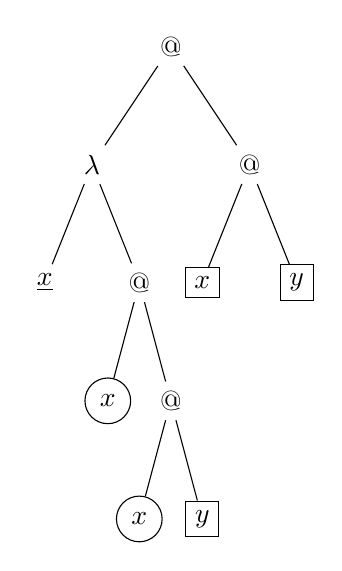
\begin{tikzpicture}
      [level 1/.style={sibling distance=20mm},
        level 2/.style={sibling distance=12mm},
          level 3/.style={sibling distance=8mm}]
      \node at (0,0) {@}
            child { node {$\lambda$}
              child { node {\underline{$x$}}}
              child { node {@}
                child { node [draw,circle] {$x$}}
                child { node {@}
                  child { node[draw,circle] {$x$}}
                  child { node[draw,rectangle] {$y$}}
}}}
            child { node {@}
              child {node[draw,rectangle] {$x$}}
              child {node[draw,rectangle] {$y$}}};
    \end{tikzpicture}
    \end{center}
    \caption{Example term illustrating the concepts of binding, bound, and free variable occurrence.  The underlined node is a binding occurrence, circled nodes are bound occurrences (bound by that sole underlined binding occurrence), and boxed nodes are free occurrences.}
    \label{fig:varocc}

\end{figure}

\section{Capture-avoiding substitution}
\label{sec:subst}

To define how $\lambda$-terms compute (Section~\ref{sec:singlebeta}
below), we need a notion of substitution, where one term $t'$ is
substituted for the free occurrences of a variable $x$ in another term
$t$.  We will use the notation $[t'/x]t$ to denote the result of this
substitution, if defined\index{substitution!capture-avoiding}.
Substitution is used to define how lambda abstractions reduce (i.e.,
compute) when applied to arguments.  We will need to substitute
arguments $t'$ for input variables $x$ in bodies $t$ of
$\lambda$-abstractions.  Note that the notation $[t'/x]t$ is part of
our meta-language discussion of $\lambda$-calculus, and not new
object-language syntax within the language of $\lambda$-calculus.
Also, it should be mentioned that one finds numerous other notations
for substitution in the literature.  For example, Church writes
$\textsf{S}^x_{t'} t$ where we are instead writing $[t'/x]t$.

Defining substitution is, arguably, the central technical issue
in the definition of the lambda calculus.  The problem is essentially
one of the proper maintenance of scoping of variable, as we will
consider next.

\subsection{Variable capture}

 The main problem in defining substitution is to ensure that a
 substitution $[t'/x]t$ avoids \emph{variable capture}, where some
 free occurrences of a variable $y$ in the term $t'$ get captured by a
 $\lambda$-abstraction of $y$ occurring in $t$.  Such a capture would
 represent a change of scoping of those occurrences in $t'$: before
 the subsitution, they were not bound by any $\lambda$-abstraction in
 $t$, but after the substitution they are.  This change of scoping is
 to be prevented.

 The simplest example of the problem is $[y/x]\lam{y}{x}$.  A naive
 (and scope-incorrect) approach to substitution would produce $\lam{y}{y}$.
 But then the occurrence of $y$ that is being substituted has changed its scoping.  Before the
 substitution, it is not bound by the displayed $\lambda\ y$, but after the
 substitution, it is.  So it has been captured.

 It is common practice, in many research works, to deal with the
 problem of variable capture by assuming that variables are implicitly
 renamed to avoid capture.  So for this example, the common practice
 would be to say that the result of $[y/x]\lam{y}{x}$ is $\lam{w}{y}$,
 for some variable $w$ different from $x$ and $y$.  This is the
 approach taken in Hindley and Seldin's book, where it is even
 specified which variable $w$ (from the countably infinite supply of
 variables) is to be used~\cite{hindley+08}.  So substitution, in
 Hindley and Seldin, is indeed a function; not all authors are so
 careful.  Additionally, most works assume what is known as
 Barendregt's variable convention: in discussing some finite set of
 lambda terms, we assume that no variable occurs both free in one of
 the terms and bound in one of the terms~\cite[Definition
   2.1.13]{barendregt85}, and further assume that variables are
 implicitly renamed to ensure this.

 In this book, I will follow a different approach, adopting a modified
 version of Church's original proposal for dealing with renaming of
 variables~\cite{church41}.  During reduction, substitution is not
 allowed in case it would lead to capture, and variables must be
 explicitly renamed first in additional reduction steps.  I have
 several reasons for pursuing this approach.  First, as variable
 binding is one of the central technical issues of lambda calculus, it
 is better, certainly when first learning the theory, not too try to
 ignore the problem by assuming things are arranged so that it never
 arises.  Second, variable binding turns out to be one of the most
 tricky aspects both for implementation of languages incorporating
 lambda calculus, and for formalizing the meta-theory of such
 language in computer theorem-proving systems.  So again, dealing with
 the problem head-on seems best, as it may encourage development of the theory
 in a way that minimizes, rather than ignores, the issue.  Perhaps
 we will find better ways to formalize lambda calculus if we isolate
 the places where renaming is needed, for example.  And finally,
 some research is directly concerned with issues of renaming
 in lambda calculus, and thus needs to be completely explicit about
 the issue.  An example is works seeking to analyze when renaming
 can always be avoided~\cite{vanoostrom23}.


\subsection{Substitution as a partial function}

Figure~\ref{fig:subst} gives the definition of substitution as a
partial function.  Recall the meta-variable convention that $x$ and
$y$ are assumed to refer to different object-language variables.  In
Equations 3 and 4 it is intended (by the ``otherwise'' at the end of Equation 2)
that $x\in\textit{FV}(t_1\ t_2)$ and $x\in\textit{FV}(\lam{y}{t})$,
respectively.  This ensures that at most one equation can be
instantiated to obtain a fact about substitution $[t_1/x]t_2$, for any
particular $t_1$, $x$, and $t_2$.  For Equations 3 and 4, let us
understand that if the right-hand side of the equation is undefined
(in some instance of the equation), then the left-hand side is, too.

\begin{figure}
\large
\[
  \begin{array}{llll}
1. &    [t'/x]x & = & t' \\
2. &    [t'/x]t & = & t, \textnormal{if }x\not\in\textit{FV}(t); \textnormal{otherwise:} \\
3. &    [t'/x](t_1\ t_2) & = & ([t'/x] t_1)\ [t'/x]t_2 \\
4. &    [t'/x]\lam{y}{t} & = & \lam{y}{[t'/x]t}, \textnormal{if } y \not\in\textit{FV}(t')
  \end{array}
\]
  \caption{Recursive definition of capture-avoiding substitution as a
    partial function.  If a recursive call is undefined then the outer
    call is also considered undefined.  The case that is similar to
    the last clause of the definition but where $y\in\textit{FV}(t')$
    is the basic undefined case.  The clauses (equations) of the definition are numbered for reference later.}
  \label{fig:subst}
  \end{figure}

\subsection{Examples}

Here are some examples of capture-avoiding substitution.

\begin{enumerate}
\item $[\lam{x}{x}/y]\lam{z}{y\ z} = \lam{z}{(\lam{x}{x})\ z}$.  In detail, labeling the equality symbol with the number of the clause from Figure~\ref{fig:subst}, and underlining the part of the term that is being changed (just for clarity), the calculation is:

  \[
  \begin{array}{ll}
    \underline{[\lam{x}{x}/y]\lam{z}{y\ z}} & =_4 \\
    \lam{z}{\underline{[\lam{x}{x}/y](y\ z)}} & =_3 \\
    \lam{z}{\underline{([\lam{x}{x}/y]y)}\ [\lam{x}{x}/y]z} & =_1 \\
    \lam{z}{(\lam{x}{x})\ \underline{[\lam{x}{x}/y]z}} & =_2 \\
    \lam{z}{(\lam{x}{x})\ z} & \
  \end{array}
  \]

\item $[(x\ x)/y]\lam{y}{x\ y} = \lam{y}{x\ y}$.  This is just by clause 2 of Figure~\ref{fig:subst}, because we are substituting for variable $y$ in a $\lambda$-abstraction which binds $y$.  The $y$ for which we are substituting cannot possibly occur free in a $\lambda$-abstraction of $y$, so substitution stops, returning the term (into which we are trying to substitute) unchanged.

\item $[\lam{y}{x\ y}/z](z\ \lam{x}{x}) = (\lam{y}{x\ y})\ \lam{x}{x}$.  In detail, we have
  \[
    \begin{array}{ll}
      \underline{[\lam{y}{x\ y}/z](z\ \lam{x}{x})} & =_3 \\
      (\underline{[\lam{y}{x\ y}/z]z})\ [\lam{y}{x\ y}/z]\lam{x}{x} & =_1 \\
      (\lam{y}{x\ y})\ \underline{[\lam{y}{x\ y}/z]\lam{x}{x}} & =_2 \\
      (\lam{y}{x\ y})\ \lam{x}{x} & \ 
    \end{array}
    \]

  \item The substitution $[x\ x/y]\lam{x}{y\ y}$ is undefined, because
    to push the substitution inside a $\lambda$-abstraction, clause 4
    of Figure~\ref{fig:subst} requires that the $\lambda$-bound
    variable (in this case $x$) is not free in the term we are
    substituting (which here is $x\ x$).  Since $x$ is free in $x\ x$,
    this means we cannot apply any of the equations of Figure~\ref{fig:subst}
    and the substitution is undefined.
\end{enumerate}

\subsection{Some properties of capture-avoiding substitution}

The following lemmas are used below.  The proofs are a bit technical, carefully applying
the definition of substitution from Figure~\ref{fig:subst}.  Dealing with the possibility
that substitutions are undefined is a somewhat tedious necessity.  Each lemma is presented
with an example, before its proof.

\begin{lemma}
\label{lem:substvargone}
  Suppose that $x\not\in\textit{FV}(t_1)$, and $[t_1/x]t_2$ is defined.  Then
  $x\not\in\textit{FV}([t_1/x]t_2)$.
\end{lemma}

\noindent\textit{Intuitive idea.} Substitution of a term $t_1$ for a variable $x$ in term $t_2$ results in a term
with no free occurrences of
$x$ (since they have all been replaced by substitution), as long as $x$ is not free in the substituted term $t_1$.

\vspace{.2cm}

\noindent\textit{Example.} Take $t_1$ to be $\lam{y}{y}$, and $t_2$ to be $x\ \lam{z}{z}$.
The conditions of the lemma are satisfied, and the result of applying the substitution
is $(\lam{y}{y})\ \lam{z}{z}$.  As stated in the lemma, $x$ does not occur free in this term.

\vspace{.2cm}

\noindent\textit{Example where the first condition does not hold.} If
we take $t_1$ to be $\lam{y}{x}$, and $t_2$ to be $x\ \lam{z}{z}$,
then the result of applying the substitution is
$(\lam{y}{x})\ \lam{z}{z}$, which does contain $x$ free.  Hence, the first condition is needed.

\begin{proof} The proof is by induction on $t_2$.
  If $x\not\in\textit{FV}(t_2)$, then by Equation 2 of Figure~\ref{fig:subst}, $[t_1/x]t_2 = t_2$, and
  hence $x\not\in\textit{FV}([t_1/x]t_2)$ (since $[t_1/x]t_2 = t_2$ and we are assuming $x\not\in\textit{FV}(t_2)$).
  So suppose $x\in\textit{FV}(t_2)$. If $t_2$ is $x$, then $[t_1/x]t_2 = t_1$,
  and the result follows by the assumption that $x\not\in\textit{FV}(t_1)$.
  If $t_2$ is $t_a\ t_b$ for some terms $t_a$ and $t_b$,
  then by the induction hypothesis, $x\not\in\textit{FV}([t_1/x]t_a)$ and $x\not\in\textit{FV}([t_1/x]t_b)$.
  So $x\not\in\textit{FV}([t_1/x](t_a\ t_b))$, since $[t_1/x](t_a\ t_b) = ([t_1/x]t_a)\ [t_1/x]t_b$ by Equation 3 of Figure~\ref{fig:subst}.
  If $t_2$ is $\lam{z}{t}$ for some $t$ and some $z$ different from $x$,
  then by the induction hypothesis, $x\not\in\textit{FV}([t_1/x]t)$.  So $x\not\in\textit{FV}(\lam{z}{[t_1/x]t})$.  The
  latter expression
    equals $[t_1/x]\lam{z}{t_2}$, since the substitution is assumed to be defined.
\end{proof}


\begin{lemma}
\label{lem:substundo}
  Suppose that $y\not\in\textit{FV}(t)$, and $[y/x]t$ is defined.  Then
  $[x/y][y/x]t$ is defined and equals $t$.
\end{lemma}

\noindent\textit{Intuitive idea.} Substituting variable $y$ for
variable $x$ and then reversing that (to substitute $x$ for $y$)
leaves the term unchanged, as long as it is legal to replace $x$ with
$y$ (avoiding capture), and as long as the original term does not have any free $y$ (since then substituting $x$ for $y$ would replace those free occurrences of $y$ with free occurrences of $x$, and the term would be different in the end).

\vspace{.2cm}

\noindent\textit{Example.} If we substitute $y$ for $x$ in $x\ \lam{x}{x}$, we get $y\ \lam{x}{x}$.  Then substituting $x$ for
$y$ restores the original term $x\ \lam{x}{x}$.

\begin{proof}
  The proof is by induction on $t$.  If $t$ is $x$, then $[x/y][y/x]x = x$.  If $x\not\in\textit{FV}(t)$,
  then $[x/y][y/x]t = [x/y]t$.  Furthermore, since $y\not\in\textit{FV}(t)$ by assumption, we have $[x/y]t = t$.
  For the rest of the proof, then, suppose $x\in\textit{FV}(t)$.

  If $t$ is $t_1\ t_2$ for some $t_1$ and $t_2$, then by the semantics of Figure~\ref{fig:subst},
  the expressions $[x/y][y/x](t_1\ t_2)$ and $([x/y][y/x]t_1)\ [x/y][y/x]t_2$ are either (a) both undefined
  or else (b) both defined and equal. Since $[y/x](t_1\ t_2)$ is defined, so are $[y/x]t_1$ and $[y/x]t_2$.
  By the induction hypothesis, then, $[x/y][y/x]t_1$ and
  $[x/y][y/x]t_2$ are defined and equal $t_1$ and $t_2$, respectively.  So $[x/y][y/x]t_1\ [x/y][y/x]t_2$ is defined and
  equals $t_1\ t_2$.  This means that it must have
  been option (b).  So $[x/y][y/x](t_1\ t_2)$ must be defined and equal to that same value, namely $t_1\ t_2$.

  Now suppose $t$ is a $\lambda$-abstraction of some variable different from $x$ (as the
  case where it is an abstraction of $x$ is covered above, by the reasoning when $x\not\in\textit{FV}(t)$).
  It is also not possible for $t$ to be $\lam{y}{t'}$ for any $t'$, because if the bound variable is $y$, the substitution
  $[y/x]\lam{y}{t'}$ is undefined, 
  So the only case we must consider is where $t$ is $\lam{z}{t'}$ for some $z$ (different from $x$ and $y$) and $t'$.

  We wish to apply the induction hypothesis to conclude that $[x/y][y/x]t'$ is defined and equals $t'$.  For this,
  we need to know first that $y\not\in\textit{FV}(t')$.  But this follows from the facts that $y\not\in\textit{FV}(\lam{z}{t'})$
  and $y \neq z$.  Second, we need to know that $[y/x]t'$ is defined.  But this follows since $[y/x]\lam{z}{t'}$ is
  defined and equals $\lam{z}{[y/x]t'}$.  Since that expression is defined, so also
  must its subexpression $[y/x]t'$ be defined.  So we can indeed apply the induction hypothesis to conclude
  that $[x/y][y/x]t'$ is defined and equals $t'$.

  Now again by the semantics of Figure~\ref{fig:subst}, since $z$ is different from $x$ and $y$, either $[x/y][y/x]\lam{z}{t'}$
  and $\lam{z}{[x/y][y/x]t'}$ are both undefined, or else both defined and equal.  But the reasoning of the previous
  paragraph shows that $\lam{z}{[x/y][y/x]t'}$ is defined (since we concluded that $[x/y][y/x]t'$ is defined)
  and equals $\lam{z}{t'}$ (since we concluded $[x/y][y/x]t' = t'$ by induction hypothesis).  Hence, $[x/y][y/x]\lam{z}{t'}$
  is also defined, and equals $\lam{z}{t'}$, as required.
\end{proof}

\section{Single-step beta-reduction}
\label{sec:singlebeta}

The central computational concept in $\lambda$-calculus is
\emph{$\beta$-reduction}, which explains how to evaluate function
calls.  A function call is an application of a $\lambda$-abstraction
to an argument.  So as a tree, it looks like:
\begin{center}
\begin{tikzpicture}
  \node at (0,0) {@}
  child { node {$\lambda$}
    child { node {$x$}}
    child { node {$t$} }}
  child { node {$t'$}};
\end{tikzpicture}
\end{center}
\noindent In textual form, it is $(\lam{x}{t})\ t'$.  The
$\beta$-axiom says that such a term reduces to $[t'/x]t$; i.e., the
result of substituting $t'$ for $x$ in
$t$, as discussed in Section~\ref{sec:subst} above.  This is only
allowed, however, if the substitution is defined.  Operationally, this
reduction of the $\beta$-redex to the result of a substitution is
called \emph{contracting} the redex; the result of substitution is called
the \emph{contractum}
\index{$\beta$-redex!contracting}\index{contractum}.  Terms of the
form $(\lam{x}{t})\ t'$, with $[t'/x]t$ defined, are called
$\beta$-redexes (for ``$\beta$-reducible
expressions'')\index{$\beta$-redex}.  Note that the requirement that
the substitution is defined is a particularity of the approach we take
in this book.

To give a formal definition of $\beta$-reduction, we will first define
what it means to reduce a single $\beta$-redex, and then, in
Section~\ref{sec:multibeta} below, define $\beta$-reduction with
multiple steps.  In both cases, we define relations between terms.  For
single-step $\beta$-reduction, the relation is denoted $\curva_\beta$.

You may recall that set theoretically, a relation is just a set of
ordered pairs, and we may equivalently write $(t,t')\in\curva$ or $t
\curva t'$ to indicate that $t$ $\beta$-reduces to $t'$.  There are
several ways to give the definition, and we will consider two.
First, we can define the $\beta$-reduction relation using a set of inference rules\index{inference rule}.
Such rules are of the form
\[
\frac{\textit{premise}_1 \ \ \cdots \ \ \textit{premise}_n}{\textit{conclusion}}
\]
\noindent It is allowed for $n$ to be $0$, in which case there are no
premises and the rule is called an \emph{axiom}.  Inference rules are
to be understood as universally quantified implications: the
conjunction of the premises implies the conclusion, for all
instantiations of the meta-variables used.  A \emph{derivation} is a
kind of tree built by instantiating the inference rules in various
ways, and then using the conclusion of one inference as the premise of
another\index{derivation}.  Such instantiated inference rules are
called \emph{inferences}\index{inference}.  A derivation is
\emph{open} if there are some premises that are not the conclusion of
any inference\index{derivation!open}.  Otherwise, it is called
\emph{closed}\index{derivation!closed}. We further stipulate that we
are only interested in facts that can be proved using finite
derivations.  

A definition of $\beta$-reduction using inference rules is given in
Figure~\ref{fig:betar}.  The leftmost rule in the figure is the
$\beta$ rule, where we require that $[t'/x]t$ is defined
in order to use the rule for inferences in a derivation.  The other
three rules express the idea that a reduction can take place anywhere
in a term.  Figure~\ref{fig:betarex} gives some example derivations.

\begin{definition}[Single-step $\beta$-reduction (rules)]
\label{def:beta}
The relation $\curva_\beta$ is the set consisting of exactly those
pairs $(t,t')$ where $t \curva_\beta t'$ is derivable (via a finite derivation) using the
rules of Figure~\ref{fig:betar}.  We write applications of the
relation in infix notation (as in those rules).  If $t \curva_\beta t'$
we say that $t$ $\beta$-reduces to $t'$.  
\end{definition}

\begin{definition}[$\beta$-redex]
  Any term of the form $(\lam{x}{t})\ t'$ is called a $\beta$-redex,
  as long as $[t'/x]t$ is defined.  Otherwise, we call such a term
  a \emph{stuck} $\beta$-redex.\index{$\beta$-redex!stuck}\index{$\beta$-redex}
  \end{definition}

\begin{definition}[nested redex]
  Suppose that a redex $R_1$ is a subterm of some other redex $R_2$.
  Then we say that $R_1$ is a nested redex (nested within $R_2$).
  \end{definition}
 
\begin{definition}[$\beta$-expansion]
\label{def:betaexpand}
  The inverse of the $\leadsto_\beta$ relation is called
  $\beta$-expansion.  If $t \leadsto_\beta t'$, we say
  that $t'$ $\beta$-expands to $t$.\index{$\beta$-expansion}
\end{definition}

\begin{figure}
  \[
  \begin{array}{lllllll}
\infer{(\lam{x}{t})\ t'\ \curva_\beta\ [t'/x]t}{\ } & \ &
\infer{\lam{x}{t}\ \curva_\beta\ \lam{x}{t'}}{t\ \curva_\beta\ t'} & \ &
\infer{t_1\ t_2\ \curva_\beta\ t_1'\ t_2}{t_1\ \curva_\beta\ t_1'} &\ &
\infer{t_1\ t_2\ \curva_\beta\ t_1\ t_2'}{t_2\ \curva_\beta\ t_2'}
  \end{array}
  \]
  \caption{Inference rules defining the $\beta$-reduction relation.  It is required that the substitution in the leftmost rule be defined, in order to use the rule.}
  \label{fig:betar}
\end{figure}

\begin{figure}
  \[
  \begin{array}{lll}
    \infer{(\lam{x}{x\ x})\ \lam{y}{y} \betar (\lam{y}{y})\ \lam{y}{y}}
          {\ }
    &
    \infer{\lam{x}{(\lam{y}{y})\ x} \betar \lam{x}{x}}
          {\infer{(\lam{y}{y})\ x \betar x}{\ }}

    &

    \infer{x\ (y\ ((\lam{x}{x})\ z)) \betar x\ (y\ z)}
          {\infer{y\ ((\lam{x}{x})\ z) \betar y\ z}
            {\infer{(\lam{x}{x})\ z \betar z}{\ }}}
  \end{array}
\]
\caption{Example derivations using the rules of Figure~\ref{fig:betar} for $\beta$-reduction.}
\label{fig:betarex}
\end{figure}

\noindent The following definition is generic, for any $R\subseteq (A\times A)$.  We will call such
a set a (binary) relation on $A$.\index{binary relation on a set}

\begin{definition}[determinism]
\label{def:det}
  An element $x$ is said to be deterministic with respect to some
  relation $R$ on a set $A$ iff for all $y$ and $y'$, if $x R y$ and
  $x R y'$ then $y = y'$.  $R$ itself is called deterministic iff
  every element of $A$ is deterministic with respect to $R$.
  Mathematically, being deterministic is the same as being a
  functional relation.  A nondeterministic relation is then simply one
  which fails to be deterministic for at least one
  $x$.\index{relation!deterministic}\index{determinism}
  \end{definition}

\begin{lemma}
  The $\leadsto_\beta$ relation is nondeterministic.
\end{lemma}
\begin{proof}
  Any term containing two non-nested $\beta$-redexes will have
  two distinct contracta.  For example, $(\lam{x}{x}\ y)\ (\lam{x}{x}\ z)$
  has distinct contracta $y\ (\lam{x}{x}\ z)$ and $(\lam{x}{x}\ y)\ z$.
  Hence, $\leadsto_\beta$ is nondeterministic.
\end{proof}

\subsection{An alternative definition using contexts}

Another way to define the same $\curva_\beta$ relation is with
contexts.  Let us first introduce the concept of \emph{grafting},
which is just substitution that does \underline{not} avoid
capture\index{grafting}.  We will write $\langle t/x\rangle t'$ for
the grafting relation (there does not seem to be a generally adopted
notation for grafting).  The definition, given in
Figure~\ref{fig:grafting}, is essentially the same as the one for substitution,
except that the last clause does not impose
any requirements on $\textit{FV}(t')$.

\begin{figure}
\large
\[
  \begin{array}{lll}
\    \langle t'/x \rangle x & = & t' \\
\    \langle t'/x \rangle t & = & t, \textnormal{if }x\not\in\textit{FV}(t); \textnormal{otherwise:} \\
\    \langle t'/x \rangle(t_1\ t_2) & = & (\langle t'/x\rangle t_1)\ \langle t'/x\rangle t_2 \\
\    \langle t'/x\rangle\lam{y}{t} & = & \lam{y}{\langle t'/x\rangle t}
  \end{array}
\]
  \caption{Recursive definition of grafting, a total function similar to substitution but intentionally allowing variable capture.}
  \label{fig:grafting}
  \end{figure}

\begin{definition}[context]
  A term $t$ is called a context iff it contains exactly one free
  occurrence of a special fixed variable $q$\index{context}.  If $t$
  is a context, then we write $\langle t'/q \rangle t$ more briefly as
  $\langle t' \rangle t$.
  \end{definition}

\noindent Using contexts, we may give the following alternative definition of the $\beta$-reduction relation:

\begin{definition}[Single-step $\beta$-reduction (contexts)]
\label{def:betactxt}
The single-step $\beta$-reduction relation
$\curva_\beta$ is alternatively defined to be the set of all ordered pairs with first component $\langle (\lam{x}{t})\ t' \rangle t''$
  and second component $\langle [t'/x]t \rangle t''$, for some $x$, $t$, $t'$, and $t''$ (with $t''$ a context and $[t'/x]t$ defined).
\end{definition}

The idea of this definition is to express that (in operational terms)
if you find a $\beta$-redex somewhere in some possibly bigger term
$t_1$, then you may reduce $t_1$ by contracting that $\beta$-redex and
then rebuilding the rest of the term $t_1$ around the contractum.  The
definition expresses finding $(\lam{x}{t})\ t'$ in possibly bigger
term $t_1$ by writing $\langle(\lam{x}{t})\ t'\rangle t''$ for $t_1$.
In other words, you have some term $t_1$ that contains a designated
occurrence of the redex, because $t_1$ is what you get when you graft
the redex in for the single occurrence of special variable $q$ in some
context $t''$.  The reason that we use grafting for this definition
instead of substitution is to allow contraction of redexes that
contain free variables that are bound in $t_1$.  We will discuss this
point further in the examples next.

\subsection{Examples}
\label{sec:betaex}

\begin{enumerate}
  \item $(\lam{x}{x\ x})\ \lam{y}{y}$ reduces to
    $(\lam{y}{y})\ \lam{y}{y}$.  For this, the meta-variables of
    Definition~\ref{def:betactxt} are instantiated thus:
    \begin{itemize}
    \item $x$ is instantiated with $x$,
    \item $t$ with $x\ x$,
    \item $t'$ with $\lam{y}{y}$
    \item $t''$ with $q$ (the special context variable)
    \end{itemize}

\item $\lam{x}{(\lam{y}{y})\ x}$ reduces to $\lam{x}{x}$.  Here the instantiations for Definition~\ref{def:betactxt} are:
    \begin{itemize}
    \item $x$ is instantiated with $y$,
    \item $t$ with $y$,
    \item $t'$ with $x$
    \item $t''$ with $\lam{x}{q}$.
    \end{itemize}

    Notice that here we really need the idea of grafting, because our
    redex contains $x$ free, which is bound in $t''$.  We want to
    allow reduction of redexes that contain variables bound outside
    the redex, and so we use grafting to specify that the $x$ in the
    redex may be bound in $t''$.  If we used substitution instead of
    grafting, this reduction would not be allowed by
    Definition~\ref{def:betactxt}, because $[(\lam{y}{y})\ x/q]\lam{x}{q}$
    is undefined (as the $x$ in $(\lam{y}{y})\ x$ would be captured
    pushing the substitution into $\lam{x}{q}$).

  \item $(\lam{x}{x\ x})\ \lam{x}{x\ x}$ reduces to that very same term.  The instantiations for Definition~\ref{def:betactxt} are:
    
    \begin{itemize}
    \item $x$ is instantiated with $x$,
    \item $t$ with $x\ x$,
    \item $t'$ with $\lam{x}{x\ x}$
    \item $t''$ with $q$.
    \end{itemize}

    We calculate the substitution $[t'/x]t$ as follows (referencing clause numbers from Figure~\ref{fig:subst}):
    \[
    \begin{array}{ll}
      \underline{[\lam{x}{x\ x} / x](x\ x)} & =_3 \\
      (\underline{[\lam{x}{x\ x} / x]x})\ [\lam{x}{x\ x} / x]x & =_1 \\
      (\lam{x}{x\ x})\ \underline{[\lam{x}{x\ x} / x]x} & =_1 \\
      (\lam{x}{x\ x})\ \lam{x}{x\ x} & \ 
    \end{array}
    \]
    \noindent This is an important basic example, because it shows
    that terms can reduce to themselves, and hence can give rise to
    infinite reductions (to be defined just below).
    \end{enumerate}

\section{Definitions using closure operators}
\label{sec:clos}

In what follows, yet a third way of defining single-step
$\beta$-reduction will prove illuminating, which is via
\textbf{closure operators} on relations.\index{closure operator}
Such an operator takes a relation $R$ and produces some new relation (let us
call it $R'$) such that $R\subseteq R'$ and $R'$ satisfies some desired property.
We will generally define closure operators using rules.

An important example in our setting is the \textbf{compatible closure}
$\curva_R$ of $R$. \index{compatible closure} The rules for this are
given in Figure~\ref{fig:compcl}.  Given any relation $R$ on terms,
$\curva_R$ is also a relation on terms, which contains $R$; i.e., if
two terms are related by $R$, then thanks to the first rule of
Figure~\ref{fig:compcl}, they are also related by $\curva_R$.  We may
call this the inclusion rule for the compatible closure. \index{inclusion rule!compatible closure}
The property it satisfies is that is closed under the syntactic constructs
of lambda calculus, in the sense expressed by the second, third, and
fourth rules of Figure~\ref{fig:compcl}.


\begin{figure}
  \[
  \begin{array}{lllllll}
\infer{t \curva_R t'}{t\ R\ t' } & \ &
\infer{\lam{x}{t}\ \curva_R\ \lam{x}{t'}}{t\ \curva_R\ t'} & \ &
\infer{t_1\ t_2\ \curva_R\ t_1'\ t_2}{t_1\ \curva_R\ t_1'} &\ &
\infer{t_1\ t_2\ \curva_R\ t_1\ t_2'}{t_2\ \curva_R\ t_2'}
  \end{array}
  \]
  \caption{Definition of compatible closure of $R$.}
  \label{fig:compcl}
\end{figure}

We may now see that if we just define the bare $\beta$ relation as in
Figure~\ref{fig:barebeta}, then we can obtain $\curva_\beta$ as the
compatible closure of $\beta$.  We may easily observe that
$\curva_\beta$ as defined this way and as defined via the rules of
Figure~\ref{fig:betar} are the same.  The definition using compatible
closure and bare $\beta$ just decomposes the rules of
Figure~\ref{fig:betar} into two parts, but is otherwise essentially
the same, except for bare $\beta$ inferences, which we will not generally
write (thus preferring the slightly more compact rules of Figure~\ref{fig:betar} for
presenting examples).

\begin{figure}
  \[
    \infer{(\lam{x}{t})\ t' \ \ \beta\ \ [t'/x]t}{\ }
  \]

  \caption{Definition of the bare $\beta$ relation, from which $\curva_\beta$ may then be defined
    via compatible closure.  This again presupposes the substitution is defined.}
\label{fig:barebeta}
\end{figure}

\begin{definition}[symmetric closure]
If $R$ is a relation, then its symmetric closure is the union of $R$ with $R^{-1}$, its inverse (i.e., the relation consisting
of those pairs $(y,x)$ where $(x,y) \in R$).\index{inverse relation}\index{symmetric closure}  When $R$ is denoted in our
meta-language using some arrow symbol like $\to$, the symmetric closure is conveniently denoted by adding an arrowhead, to get
something like $\leftrightarrow$.
\end{definition}

A final closure operator commonly used in Computer Science is the reflexive transitive closure $R^*$ of relation $R$, defined in Figure~\ref{fig:rtcl}.\index{reflexive-transitive closure}
We will use this in the definition of multi-step $\beta$-reduction below.  The first rule may be called the inclusion rule,
the second the reflexivity rule, and the third the transitivity rule.\index{inclusion rule!reflexive-transitive closure}
Note that we are not taking multi-step $\beta$-reduction
to be just $\leadsto_\beta^*$, as this relation does not allow renaming of local variables, the subject we turn to in Section~\ref{sec:alpha}.

\begin{figure}
  \[
  \begin{array}{lllllll}
    \infer{t\,R^*\,t'}{t\,R\,t'}&\,&
    \infer{t\,R^*\,t}{\,}&\,&
    \infer{t_1\,R^*\,t_3}{t_1\,R^*\,t_2 & t_2\,R^*\,t_3}
  \end{array}
  \]
  \caption{Definition of the reflexive, transitive closure $R^*$ of relation $R$.}
  \label{fig:rtcl}
  \end{figure}

\subsection{Some properties of the closure operators}

In some of the proofs later in the book, we will make use of some properties
of the closure operators above.

\begin{lemma}[monotonicity of star]
\label{lem:starmono}
  For relations $R$ and $S$ on set $A$, if $R \subseteq S$, then $R^* \subseteq S^*$.
\end{lemma}
\begin{proof}
  Assume $t\ R^*\ t'$, and show $t\ S^*\ t'$.  The proof is by induction
  on the derivation of $t\ R^*\ t'$.
  \case{ }
  \[
  \infer{t\ R^*\ t'}{t\ R\ t'}
  \]
  \noindent Since $R \subseteq S$, we have $t\ S\ t'$ from $t\ R\ t'$, and
  then obtain $t\ S^*\ t'$ by applying this same inclusion rule.

  \case{ }
  \[
  \infer{t\ R^*\ t}{\ }
  \]
  \noindent Note that in this case, the inference used forces $t'$ to equal $t$.
  Using this same reflexivity rule, we derive $t\ S^*\ t$.

  \case{ }
  \[
  \infer{t\ R^*\ t'}{t\ R^*\ t'' & t''\ R^*\ t'}
  \]
  \noindent We may construct this derivation, where uses of the
  induction hypothesis are indicated with inferences labeled
  \textit{IH}.  These are not inferences by a rule of
  Figure~\ref{fig:rtcl}, but rather indicate that invocation of the
  induction hypothesis is legal for the fact above the bar and
  produces the result shown below the bar.
  \[
  \infer{t\ S^*\ t'}{\infer[\textit{IH}]{t\ S^*\ t''}{t\ R^*\ t''} & \infer[\textit{IH}]{t''\ S^*\ t'}{t''\ R^*\ t'}}
  \]
\end{proof}

\begin{lemma}[compatible closure preserves symmetry]
\label{lem:compclsymm}
  If $R$ is symmetric, then $\leadsto_R$ is also.
\end{lemma}
\begin{proof}
  Given symmetric $R$, assume $t \leadsto_R t'$ and show $t' \leadsto_R t$.
  The proof is by induction on the assumed derivation of $t \leadsto_R t'$ (using the rules of Figure~\ref{fig:compcl}).

  \case{ }
  \[
  \infer{t \curva_R t'}{t\ R\ t' }
  \]
  \noindent We construct this derivation, where $t'\ R\ t$ is deduced by symmetry of $R$:
  \[
  \infer{t' \curva_R t}{\infer{t'\ R\ t}{t\ R\ t'}}
  \]

  \case{ }
  \[
  \infer{\lam{x}{t}\ \curva_R\ \lam{x}{t'}}{t\ \curva_R\ t'}
  \]
  \noindent We construct:
  \[
  \infer{\lam{x}{t'}\ \curva_R\ \lam{x}{t}}{\infer[\textit{IH}]{t'\ \curva_R\ t}{t\ \curva_R\ t'}}
  \]

  \case{ }
  \[
  \infer{t_1\ t_2\ \curva_R\ t_1'\ t_2}{t_1\ \curva_R\ t_1'}
  \]
  \noindent We construct:
  \[
  \infer{t_1'\ t_2\ \curva_R\ t_1\ t_2}{\infer[\textit{IH}]{t_1'\ \curva_R\ t_1}{t_1\ \curva_R\ t_1'}}
  \]

  \case{ }
  \[
  \infer{t_1\ t_2\ \curva_R\ t_1\ t_2'}{t_2\ \curva_R\ t_2'}
  \]
  \noindent We construct:
  \[
  \infer{t_1\ t_2'\ \curva_R\ t_1\ t_2}{\infer[\textit{IH}]{t_2'\ \curva_R\ t_2}{t_2\ \curva_R\ t_2'}}
  \]
  
  \end{proof}

\begin{lemma}[reflexive-transitive closure preserves symmetry]
\label{lem:rtclsymm}
  If $R$ is symmetric, then $R^*$ is also.
\end{lemma}
\begin{proof}
  Given symmetric $R$, assume $t\,R^*\,t'$ and show $t'\,R^*\,t$.  The proof is by induction
  on the assumed derivation of $t\,R^*\,t'$ (using the rules of Figure~\ref{fig:rtcl}).
  \case{ }
  \[
  \infer{t\,R^*\,t'}{t\,R\,t'}
  \]
  \noindent We construct this derivation, where $t'\,R\,t$ is deduced by symmetry of $R$:
  \[
  \infer{t'\,R^*\,t}{\infer{t'\,R\,t}{t\,R\,t'}}
  \]

  \case{ }
  \[
  \infer{t\,R^*\,t}{\,}
  \]
  \noindent In this case $t = t'$ and we thus have $t'\,R^*\,t$ by this very inference.

  \case{ }
  \[
  \infer{t_1\,R^*\,t_3}{t_1\,R^*\,t_2 & t_2\,R^*\,t_3}
  \]
  \noindent We construct:
  \[
  \infer{t_3\,R^*\,t_1}{\infer[\textit{IH}]{t_3\,R^*\,t_2}{t_2\,R^*\,t_3} & \infer[\textit{IH}]{t_2\,R^*\,t_1}{t_1\,R^*\,t_2}}
  \]
  \end{proof}

\begin{lemma}[reflexive-transitive closure preserves compatibility]
\label{lem:comprtc}
  Suppose $R$ is a relation on terms, and consider $\leadsto_R^*$.
  Then the relations $\leadsto_R^*$  and its compatible closure $\leadsto_{\leadsto_R^*}$ are the same.
\end{lemma}
\begin{proof}
  Since $\leadsto_R^*\ \subseteq\ \leadsto_{\leadsto_R^*}$ by the inclusion rule
  of Figure~\ref{fig:compcl}, it suffices to show $\leadsto_{\leadsto_R^*}\ \subseteq\ \leadsto_R^*$.
  So assume $t\ (\leadsto_{\leadsto_R^*}\ t'$ and show $t \leadsto_R^* t'$.  The proof
  is by induction on the assumed derivation (with the rules of Figure~\ref{fig:compcl}).

  \case{ } 
  \[
  \infer{t\ (\leadsto_R^*)_R\ t'}{t \leadsto_R^* t'}
  \]
  \noindent The desired conclusion for this inclusion inference is its premise: $t \leadsto_R^* t'$.

  \case{ }
  \[
  \infer{\lam{x}{t}\ (\leadsto_R^*)_R\ \lam{x}{t'}}{t\ (\leadsto_R^*)_R\ t'}
  \]
  \noindent By the induction hypothesis, we have $t\ \leadsto_R^*\ t'$.  We
  proceed by inner induction on the derivation of this fact, to show
  the desired $\lam{x}{t}\ \leadsto_R^*\ \lam{x}{t'}$.

  \case{ (inner)}
  \[
  \infer{t \leadsto_R^* t'}{t \leadsto_R t'}
  \]
  \noindent We construct
  \[
  \infer{\lam{x}{t} \leadsto_R^* \lam{x}{t'}}
        {\infer{\lam{x}{t} \leadsto_R \lam{x}{t'}}
          {t \leadsto_R t'}}
  \]

  \case{ (inner)} 
  \[
  \infer{t \leadsto_R^* t}{\ }
  \]
  \noindent This case forces $t' = $.  We construct the following, again applying the reflexivity rule:
  \[
  \infer{\lam{x}{t} \leadsto_R^* \lam{x}{t}}{\ }
  \]

  \case{ (inner)}
  \[
  \infer{t \leadsto_R^* t'}{t \leadsto_R^* t'' & t'' \leadsto_R^* t'}
  \]
  \noindent We construct the following, applying the transitivity rule:
  \[
  \infer{\lam{x}{t} \leadsto_R^* \lam{x}{t'}}{\infer[\textit{IH}]{\lam{x}{t} \leadsto_R^* \lam{x}{t''}}{t \leadsto_R^* t''}
                                             & \infer[\textit{IH}]{\lam{x}{t''} \leadsto_R^* \lam{x}{t'}}{t'' \leadsto_R^* t'}}
  \]

  \noindent This concludes the inner induction for the case where the compatible closure rule is the $\lambda$-abstraction rule.

\todo{need to fill in proofs for application rules}

  \end{proof}
        
  

\section{Alpha-equivalence}
\label{sec:alpha}

\begin{figure}
  \[
   \infer[y\not\in\textit{FV}(t)]{\lam{x}{t}\ \ \alpha\ \ \lam{y}{[y/x]t}}{\ }
  \]

  \caption{Definition of the bare $\alpha$ relation, from which $\curva_\alpha$ is then defined
    via compatible closure.  This presupposes the substitution in the rule is defined.}
\label{fig:barealpha}
\end{figure}

The intention with $\lambda$-abstraction is that it introduces a
variable with local scope, to refer to input arguments.  Terms that
are the same except for choice of these local variables intuitively
should be equivalent in some way.  In this section, we define this
notion of equivalence, which historically is called
$\alpha$-equivalence\index{$\alpha$-equivalence}.  The intention is
that two terms $t_1$ and $t_2$ are $\alpha$-equivalent iff one can
perform safe renamings to different $\lambda$-subterms of $t_1$ to
obtain $t_2$.  A safe renaming of a subterm $\lam{x}{t}$ is
$\lam{y}{[y/x]t}$ where $y\not\in\textit{FV}(t)$ and the substitution
is defined\index{renaming!safe}.  Safe renamings
change binding and their corresponding bound occurrences of $x$ into
$y$, where $y$ is not free in the body $t$.  By requiring $y$ not to
be free in $t$, we ensure that we cannot accidentally capture free
occurrences of $y$ in $t$, which would be an example of the scope
confusion we are trying to avoid with capture-avoiding substitution.

To define $\alpha$-equivalence, we begin with the bare $\alpha$
relation of Figure~\ref{fig:barealpha}.  This allows us to rename the
variable $x$ bound by $\lam{x}{t}$ to any $y$ which is not free in
$t$, and for which the substitution $[y/x] t$ is defined.  If $y$ does
not have any occurrences whatsoever in $t$, then it satisfies these
two conditions.  Those conditions are required to ensure that we do
not rename $x$ to some variable which either would capture some free
variable of $t$ or which would itself be captured when replacing $x$
with it.

Next we apply the compatible closure (Figure~\ref{fig:compcl}), to get
$\curva_\alpha$.  This allows us to perform such a renaming anywhere
we want in a term.  Finally, we take the reflexive transitive closure,
so that we can perform any finite sequence of renamings.  This gives
us the final definition:

\begin{definition}[$\alpha$-equivalence]
\label{def:alpha}
  The relation $=_\alpha$, called $\alpha$-equivalence, is $(\leadsto_\alpha)^*$.
  \end{definition}

\subsection{Examples}

\begin{enumerate}
\item $\lam{x}{x} \curva_\alpha \lam{y}{y}$, for any $y$ different from $x$.  In general, we can see that $\curva_\alpha$ is nondeterministic.
\item $\lam{x}{\lam{y}{z\ x}}$ is $\alpha$-equivalent to $\lam{y}{\lam{w}{z\ y}}$, by combining (using the rules of Figure~\ref{fig:rtcl})
  the following $\curva_\alpha$ steps:
  \begin{itemize}
  \item $\lam{x}{\lam{y}{z\ x}} \curva_\alpha \lam{x}{\lam{w}{z\ x}}$, proved with this derivation (using the rules of Figure~\ref{fig:compcl} and Figure~\ref{fig:barealpha}):
    \[
    \infer{\lam{x}{\lam{y}{z\ x}} \curva_\alpha \lam{x}{\lam{w}{z\ x}}}
          {\infer{\lam{y}{z\ x} \curva_\alpha \lam{w}{[w/y](z\ x)}}{\infer{\lam{y}{z\ x} \ \alpha \ \lam{w}{[w/y](z\ x)} }{\ }}}
          \]
    
    \item $\lam{x}{\lam{w}{z\ x}} \curva_\alpha \lam{y}{\lam{w}{z\ y}}$.
          
  \end{itemize}
  We combine those derivations into a single derivation for the $\alpha$-equivalence in Figure~\ref{fig:alphaexa}.
\item $\lam{x}{\lam{y}{y\ x}} =_\alpha \lam{y}{\lam{x}{x\ y}}$, but this is slightly tricky.  It is similar to the problem of swapping the values of two variables in an imperative programming language, and uses the same solution: introduce an auxiliary variable.  So we have these $\curva_\alpha$ steps:
  \begin{itemize}
  \item $\lam{x}{\underline{\lam{y}{y\ x}}} \curva_\alpha \lam{x}{\lam{w}{w\ x}}$
  \item $\underline{\lam{x}{\lam{w}{w\ x}}} \curva_\alpha \lam{y}{\lam{w}{w\ y}}$
  \item $\lam{y}{\underline{\lam{w}{w\ y}}} \curva_\alpha \lam{x}{\lam{y}{y\ x}}$
    \end{itemize}
\end{enumerate}

\begin{figure}
  \[
  \infer{\lam{x}{\lam{y}{z\ x}} \curva_\alpha^* \lam{y}{\lam{w}{z\ y}}}
    {\infer{\lam{x}{\lam{y}{z\ x}} \curva_\alpha^* \lam{x}{\lam{w}{z\ x}}}
        {\infer{\lam{x}{\lam{y}{z\ x}} \curva_\alpha \lam{x}{\lam{w}{z\ x}}}
          {\infer{\lam{y}{z\ x} \curva_\alpha \lam{w}{[w/y]z\ x}}{\infer{\lam{y}{z\ x} \ \alpha\  \lam{w}{[w/y]z\ x}}{\ } }}} & 
        \infer{\lam{x}{\lam{w}{z\ x}} \curva_\alpha^* \lam{y}{\lam{w}{z\ y}}}
              {\infer{\lam{x}{\lam{w}{z\ x}} \curva_\alpha \lam{y}{\lam{w}{[y/x](z\ x)}}}{\infer{\lam{x}{\lam{w}{z\ x}} \ \alpha\  \lam{y}{\lam{w}{[y/x](z\ x)}}}{\ } }}}
    \]
\caption{Example derivation of an $\alpha$-equivalence, using the rules of Figures~\ref{fig:rtcl}, Figure~\ref{fig:compcl}, and~\ref{fig:barealpha}. Naturally, the passage from an $\alpha$ step to a $\curva_\alpha$ step at the top parts of the derivation is rather redundant, and we may safely omit the bare $\alpha$ inferences in other examples.} 
\label{fig:alphaexa}
\end{figure}

\subsection{Properties of $\alpha$-equivalence}

\begin{lemma}
\label{lem:alphasymm}
  $\alpha$ is symmetric.
\end{lemma}
\begin{proof} Suppose we have $t_1\ \alpha\ t_2$.  The only way this can happen,
  with the sole rule for the bare $\alpha$ relation (Figure~\ref{fig:barealpha})
  is if $t_1$ is of the form $\lam{x}{t}$ for some variable $x$ and term $t$, and $t_2$
  is of the form $\lam{y}{[y/x]t}$ with $y\not\in\textit{FV}(t)$ and $[y/x]t$ defined.
  We must show that under these conditions, $t_2\ \alpha\ t_1$.  This can be proved
  using the rule for bare $\alpha$ by instantiating the meta-variables in that rule
  as follows:
  \begin{itemize}
  \item $x$ is instantiated with $y$
  \item $y$ is intantiated with $x$
  \item $t$ is instantiated with $[y/x]t$
  \end{itemize}
  \noindent With those instantiations, we obtain this fact from the rule, if the
  several conditions required by the rule hold (which we will check next):
  \[
  \lam{y}{[y/x]t}\ \ \alpha\ \lam{x}{[x/y][y/x]t}
  \]
  \noindent By Lemma~\ref{lem:substundo}, $\lam{x}{[x/y][y/x]t}$ is defined and equal to $\lam{x}{t}$,
  so we indeed have $t_2\ \alpha\ t_1$.  That lemma requires that $y\not\in\textit{FV}(t)$ and that $[y/x]t$ is defined; both
  of these hold by assumption from the original application of the rule for bare $\alpha$.  The requirement, on this
  new bare-$\alpha$ inference, that $x\not\in\textit{FV}([y/x]t)$ follows
  by Lemma~\ref{lem:substvargone}, since $x\not\in\textit{FV}(y) = \{y\}$ (because $x\neq y$
  by our convention on meta-variables for variables).

  \end{proof}


\begin{corollary}
  $=_\alpha$ is symmetric, so $=_\alpha$ is indeed an equivalence relation.
\end{corollary}
\begin{proof}
  Since bare $\alpha$ is symmetric (Lemma~\ref{lem:alphasymm}), we may apply Lemma~\ref{lem:compclsymm} to conclude
  that $\leadsto_\alpha$ is symmetric.  Then we may apply Lemma~\ref{lem:rtclsymm} to conclude that $(\leadsto_\alpha)^*$ (which
  we defined $\alpha$-equivalence to be in Definition~\ref{def:alpha}) is
  symmetric.
\end{proof}


\section{Multi-step beta-reduction}
\label{sec:multibeta}

Having defined single-step $\beta$-reduction
(Definition~\ref{def:beta}, or alternatively
Definition~\ref{def:betactxt}) and $\alpha$-equivalence
(Definition~\ref{def:alpha}), we will combine these two concepts for a
relation expressing the idea of computation: that is, performing a
sequence of $\beta$-reductions, where safe renaming of variables is
allowed between steps to enable computation to proceed (where it could
otherwise be stuck due to undefinedness of a substitution).  This can
be done concisely using the closure operators introduced above.
First, though, we should recall the definition of relational
composition:

\begin{definition}[relational composition]
  If $R$ and $S$ are (binary) relations, then by $R S$ we denote their
  composition, namely,
  \[
  \{ (x,z)\ |\ \exists\ y.\ (x,y)\in R \ \wedge\ (y,z) \in S \}
  \]
  \noindent That is, the set of pairs $(x,z)$ such that there exists some $y$ with
  $(x,y) \in R$ and $(y,z)\in S$.
\end{definition}

\begin{definition}[single step $\beta$-reduction with renaming]
  For compact notation below, let us write $\betaa$ for $=_\alpha \betar =_\alpha$
  (i.e., the relational composition of
$\alpha$-equivalence, followed by single-step $\beta$-reduction,
followed by $\alpha$-equivalence).  This is called single-step
$\beta$-reduction with renaming.
\end{definition}

A single $\beta$-reduction step with renaming allows one to perform some (possibly zero)
renamings, then take a $\betar$-step, and then perform another set of renamings.
We are generally interested in taking multiple steps of $\betaa$, using $\betaa^*$, which
we will call multi-step $\beta$-reduction with renaming.\index{multi-step $\beta$-reduction with renaming}
It is often useful to identify a sequence of terms underlying a
multi-step $\beta$-reduction with renaming, as follows:

\begin{definition}[$\betaa$-reduction sequence]
\label{def:betars}
  A $\betaa$-reduction sequence is a finite list of terms
  $t_1,\ldots,t_k$, such that for each $i\in\{1,\ldots,k-1\}$,
  $t_i \betaa t_{i+1}$.  We may write such
  a sequence as
  \[
  t_1 \betaa \ldots \betaa t_k
  \]
  We say this is a $\betaa$-reduction sequence for $t_1\betaa^* t_k$.
\end{definition}

Note that there may be more than one $\betaa$-reduction sequence
for a given multi-step reduction, because different intermediate
renamings may be possible.

\subsection{Examples}

\begin{enumerate}
\item The following shows that $(\lam{x}{\lam{y}{x\ x}})\ \lam{x}{y}$
  multi-step $\beta$-reduces to $\lam{w}{y}$.  For the $=_\alpha$
  step, I am underlining the underlying $\alpha$-step that has been
  taken, and similarly for the $\curva_\beta$ steps, I am
  underlining the underlying $\beta$-step that has been taken (with
  $\alpha$ and $\beta$ of Figures~\ref{fig:barealpha} and~\ref{fig:barebeta}).

  \[
\begin{array}{ll}
  (\lam{x}{\underline{\lam{y}{x\ x}}})\ \lam{x}{y} & =_\alpha \\
  \underline{(\lam{x}{\lam{w}{x\ x}})\ \lam{x}{y}} & \curva_\beta \\
  \lam{w}{\underline{(\lam{x}{y})\ \lam{x}{y}}} & \curva_\beta \\
  \lam{w}{y} & \ 
\end{array}
\]
  A $\betaa$-reduction sequence (as in Definition~\ref{def:betars}) for this is
\[
\begin{array}{ll}
  (\lam{x}{\underline{\lam{y}{x\ x}}})\ \lam{x}{y} \betaa \\
  \lam{w}{\underline{(\lam{x}{y})\ \lam{x}{y}}} & \betaa \\
  \lam{w}{y} & \
\end{array}
\]

The following reduction sequence is different, because in the second line the first
$\lambda$-bound variable is $p$ instead of $w$:
\[
\begin{array}{ll}
  (\lam{x}{\underline{\lam{y}{x\ x}}})\ \lam{x}{y} \betaa \\
  \lam{p}{\underline{(\lam{x}{y})\ \lam{x}{y}}} & \betaa \\
  \lam{w}{y} & \
\end{array}
\]

\end{enumerate}

Note that we may reasonably generalize this notion of
$\betaa$-reduction sequence to other relations besides
$\betaa$.  We can call these \emph{relational sequences}.  For
example, a $=_\alpha$-sequence is a list of terms where consecutive
terms are related by $=_\alpha$. Or a bare $\beta$ sequence would
be a list of terms where consecutive terms are related by the bare $\beta$
relation of Figure~\ref{fig:barebeta}.

\begin{definition}[maximal relational sequence]
  An $R$-sequence $t_1\ R \ \cdots\ R\ t_n$ is called maximal iff
  there is no $t'$ with $t_n\ R \ t'$.
  \end{definition}

A maximal $\beta$-reduction sequence is one that ends in a term
which cannot be single-step $\beta$-reduced (with renaming).  Such
a term is called a $\beta$-normal form:

\begin{definition}[$\beta$-normal form]
\label{def:betanf}
  A term $t$ is in $\beta$-normal form iff there is no $t'$ such
  that $t\betaa t'$.  This is sometimes denoted $t \not\betaa$.
  One sometimes writes $t\betaa^! t'$ to mean
  that $t\betaa^*t'$ where $t'$ is $\beta$-normal.\index{$\beta$-normal}
\end{definition}

As we have been doing, we may generalize this notion for any relation.
So a bare $\beta$-normal form, for example, is a term which is not a
live $\beta$-redex.  And a $\curva_\alpha$-normal form is a term which
cannot be renamed; i.e., a term containing no $\lambda$-abstraction
(since all $\lambda$-abstractions can be renamed).

\begin{definition}[normalizing]
\label{def:normalizing}
  A term $t$ is $R$-normalizing, denoted $t \downarrow_R$, iff there is an $R$-normal form $t'$ with $t\ R^*\ t'$.
  If an $R$-reduction sequence ends in an $R$-normal form, we call the sequence $R$-normalizing as well.
  If $R$ is left off, we assume it is $\betaa$.\index{normalizing term}
\end{definition}

So a normalizing term $t$ is one which has a multi-step $\beta$-reduction to a term
which then does not reduce (with $\betaa$).  

\begin{definition}[non-normalizing]
\label{def:nonnorm}
  If term $t$ is not $R$-normalizing, we call it $R$-non-normalizing, denoted $t \uparrow_R$.
  As above, if $R$ is left off, we assume it is $\betaa$.\index{normalizing term}
\end{definition}

We will see a well-known example of a non-normalizing term in the next
chapter ($\Omega$, Section~\ref{sec:basicfuncs}).  Finally, it is also
sometimes of interest to consider the equivalence closure of
$\beta$-reduction with renaming:

\begin{definition}{$\beta$-equivalence}
  We define $\approx$ as the equivalence closure of $\curva$; i.e., $=_{\curva}$.
  \end{definition}

\section{Exercises}

\subsection{Basic syntax}

\begin{enumerate}

  \item For each of the following terms, add parentheses to disambiguate
between possible parses following the parsing convention (as in
Figure~\ref{fig:exampleterms}), and then draw the term in tree form.

\begin{enumerate}
\item $\lam{y}{y\ y\ y}$
\item $\lam{x}{x\ a\ \lam{q}{x\ q}}$
\item $(\lam{x}{x\ x})\ \lam{x}{x\ x\ x}$
\item $\lam{f}{\lam{a}{f\ (f\ (f\ a))}}$
\item $(\lam{x}{x\ x})\ \lam{y}{x}$
\end{enumerate}

\item For each term shown in tree form below, write that term in
  textual form, using at least those parentheses (more are fine if you
  wish) required by our parsing conventions to describe the tree
  structure correctly.


  \begin{enumerate}
  \item

    \

    \begin{tikzpicture}
  \node at (0,0) {@}
  child { node {$x$}}
  child { node {@}
      child {node {$y$}}
      child { node {$\lambda$}
    child { node {$x$}}
    child { node {$x$}}}};
 \end{tikzpicture}

  \item

    \

    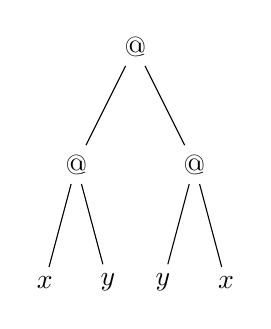
\begin{tikzpicture}
      [level 1/.style={sibling distance=15mm},
        level 2/.style={sibling distance=8mm}]
  \node at (0,0) {@}
  child { node {@}
      child {node {$x$}}
      child { node {$y$} }}
  child { node {@} 
      child {node {$y$}}
      child { node {$x$} }};
 \end{tikzpicture}

  \item

    \

    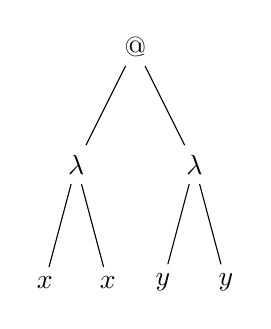
\begin{tikzpicture}
      [level 1/.style={sibling distance=15mm},
        level 2/.style={sibling distance=8mm}]
  \node at (0,0) {@}
  child { node {$\lambda$}
      child {node {$x$}}
      child { node {$x$} }}
  child { node {$\lambda$} 
      child {node {$y$}}
      child { node {$y$} }};
 \end{tikzpicture}


  \item

    \

    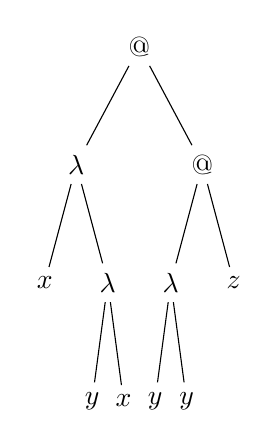
\begin{tikzpicture}
      [level 1/.style={sibling distance=16mm},
        level 2/.style={sibling distance=8mm},
          level 3/.style={sibling distance=4mm}]
  \node at (0,0) {@}
  child { node {$\lambda$}
      child {node {$x$}}
      child { node {$\lambda$}
        child {node {$y$}}
        child {node {$x$}}}}
  child { node {@}
    child { node {$\lambda$} 
        child {node {$y$}}
        child { node {$y$} }}
    child { node {$z$}}};
 \end{tikzpicture}



  \item

    \

    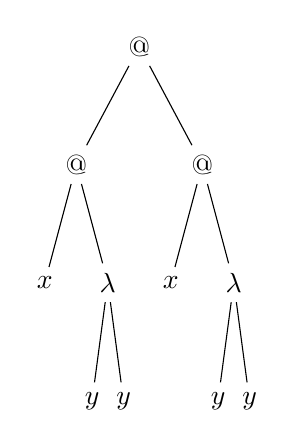
\begin{tikzpicture}
      [level 1/.style={sibling distance=16mm},
        level 2/.style={sibling distance=8mm},
          level 3/.style={sibling distance=4mm}]
  \node at (0,0) {@}
  child { node {@}
      child {node {$x$}}
      child { node {$\lambda$}
        child {node {$y$}}
        child {node {$y$}}}}
  child { node {@}
    child { node {$x$}}
    child { node {$\lambda$} 
        child {node {$y$}}
        child { node {$y$} }}};
 \end{tikzpicture}


  \end{enumerate}


  \end{enumerate}
  
\subsection{Kinds of variable occurrences}

 For each of the given terms, draw them in tree form and then
 indicate, in the same way as in Figure~\ref{fig:varocc}, which
 variable occurrences are binding (please underline), which are bound
 (please circle), and which are free (please box):
\begin{enumerate}

\item $y$

\vspace{.5cm}
\item $\lambda\, y.\ y$

\vspace{.5cm}
\item $(\lambda\, x.\, x\ x)\ y$

\vspace{.5cm}
\item $\lambda\, x.\, (\lambda\, y.\, x)\ y$

\vspace{.5cm}
\item $\lambda\, y.\, \lambda\, z.\, x\ y\ y\ (w\ z)$

\vspace{.5cm}
\end{enumerate}

\subsection{Capture-avoiding substitution}

For each of the following, write the result of the substitution or that it is undefined.

\begin{enumerate}
\item $[x/y]\lam{z}{y\ y}$
  
  \vspace{.5cm}

\item $[(x\ x)/y]\lam{z}{z\ (y\ y)}$

  \vspace{.5cm}

\item $[(x\ x)/y]\lam{y}{z\ y}$

  \vspace{.5cm}

\item $[\lam{x}{x}/y]\lam{z}{y\ \lam{y}{y\ z}}$

  \vspace{.5cm}

\item $[\lam{x}{y}/z]\lam{y}{y\ z}$
  \end{enumerate}


\subsection{Single-step $\beta$-reduction}

\begin{enumerate}
  \item Each of the following reductions is allowed by Definition~\ref{def:betactxt}.  For each reduction, indicate the instantiations of the meta-variables $x$, $t$, $t'$, and $t''$ of Definition~\ref{def:betactxt} (as in the examples in Section~\ref{sec:betaex}).
    \begin{enumerate}
    \item $\lam{x}{(\lam{y}{y})\ \lam{z}{z}}\ \betar \lam{x}{\lam{z}{z}}$
      \vspace{.5cm}
    \item $(\lam{y}{y})\ (z\ z)\ z\ \betar z\ z\ z$
      \vspace{.5cm}
    \item $z\ (\lam{y}{(\lam{z}{z\ z})\ (y\ y)}) \betar z\ \lam{y}{y\ y\ (y\ y)}$
      \vspace{.5cm}
    \item $(\lam{x}{\lam{y}{x\ x}})\ (z\ \lam{z}{z}) \betar \lam{y}{z\ (\lam{z}{z})\ (z\ \lam{z}{z})}$
      \vspace{.5cm}
    \item $(\lam{x}{\lam{y}{y}})\ z \betar \lam{y}{y}$
      \vspace{.5cm}
    \end{enumerate}

  \item Write derivations using the rules of Figure~\ref{fig:betar} for the $\beta$-reductions of parts (a), (b), (c) of the previous problem.

   \end{enumerate}

\subsection{$\alpha$-equivalence}

For each pair of terms, indicate whether or not they are $\alpha$-equivalent:
\begin{enumerate}
\item $\lam{x}{\lam{y}{y\ x}}$ and $\lam{x}{\lam{x}{y\ x}}$
  \vspace{.5cm}
\item $x\ \lam{y}{x}$ and $x\ \lam{w}{x}$
  \vspace{.5cm}
\item $x\ \lam{y}{x}$ and $y\ \lam{x}{y}$
  \vspace{.5cm}
\item $\lam{z}{(\lam{x}{x\ z})\ \lam{y}{z\ y}}$ and $\lam{q}{(\lam{y}{y\ q})\ \lam{y}{q\ y}}$
  \vspace{.5cm}
\end{enumerate}

\subsection{Multi-step $\beta$-reduction}

\begin{enumerate}

\item Write maximal $\curva$-reduction sequences starting with the given term.  Be careful with your renamings!

\begin{enumerate}
\item $\lam{y}{(\lam{x}{\lam{y}{x\ (x\ y)}})\ \lam{x}{y\ x}}$
  \vspace{.5cm}
\item $\lam{x}{\lam{y}{(\lam{z}{\lam{y}{\lam{x}{z\ z}}})\ \lam{z}{x\ y}}}$
  \vspace{.5cm}
\end{enumerate}

% answer: \delta app (in terms of Chapter 2)
\item Find an example of a term $t$ and number $n$ of $\beta$-steps where
  \begin{itemize}
  \item there exists a term $t'$ such that $t (=_\alpha\ \leadsto_\beta^n\ =_\alpha\ \leadsto_\beta) t'$, but
  \item there does not exist a term $t'$ such that $t (=_\alpha\ \leadsto_\beta^{n+1}) t'$.
  \end{itemize}
  \noindent In other words, this problem asks you to find an example of a term where a second $\alpha$-equivalence step is required in order to
  complete a sequence of $\beta$-reductions.  As a hint (because the problem is a bit tricky):
  \begin{itemize}
  \item If all bound and free variables are distinct from each other, then it is never necessary to rename to perform a single $\beta$-reduction, so it might seem like an initial $=_\alpha$-step would suffice to obviate any subsequent renamings... 
    \item ...but it is not! Ask yourself if there is a way that starting with a term where all bound and free variables are distinct from each other, one could arrive at a term that does not have that property; and then use this to construct a term where a second $=_\alpha$-step is required.

  \end{itemize}
\end{enumerate}

\chapter{Programming in Lambda Calculus}
\label{ch:prog}

\section{Basic functions}
\label{sec:basicfuncs}

Let us consider a few basic lambda terms that are useful for
programming in lambda calculus.  We will give names to the terms we
consider, as meta-linguistic abbreviations.  Let us use the syntax $N
:= t$ to indicate (in our meta-language) that we wish to use name $N$
as an abbreviation for term $t$.  In all cases, our choice of names
will be justified by the behavior of the term when applied to various
arguments.  By behavior, I mean the term's $\beta$-reductions.

\paradef{.5}{The identity function.} 
\[
\textit{id} := \lam{x}{x}
\]
\noindent This term really does behave like the mathematical
(set-theoretic, let us say) identity function, since if we apply
\textit{id} to anything, we just get back that same value.\index{identity \textit{id}}  We have

\[
\textit{id}\ t \ \ \betaa^* \ \ t
\]

\paradef{0}{Self-application operator.}
\[
\delta := \lam{x}{x\ x}
\]
\noindent This operator applies input $x$ to $x$. \index{self-application $\delta$}
We also have
\[
\Omega := \delta\ \delta
\]
\noindent This term has no normal form, reducing forever to itself:\index{diverging term $\Omega$}
\[
\begin{array}{ll}
  \underline{\delta}\ \delta & = \\
  \underline{(\lam{x}{x\ x})\ \delta} & \betaa \\
  \delta\ \delta &\
\end{array}
\]

\paradef{0}{Composition.}
\[
\textit{compose} := \lam{f}{\lam{g}{\lam{x}{f\ (g\ x)}}}
\]
\noindent This term can be applied to any terms $f$ and $g$, and it
will return a term that behaves like their composition: it applies $f$
after $g$ to its input $x$.  It is nice to borrow mathematical notation for
function composition and write $f \circ g$ for $\textit{compose}\ f\ g$.
Here are a few examples using \textit{compose}:\index{composition \textit{compose} (or $\circ$)}
\begin{itemize}
\item $\textit{id} \circ \textit{id} \ \ \betaa^*\ \ \textit{id}$
\item $\delta\circ \delta \ \ \betaa^*\ \ \lam{x}{x\ x\ (x\ x)}$:
\[
\begin{array}{ll}
  \underline{\delta\circ \delta} & = \\
  \underline{\textit{compose}}\ \delta\ \delta & = \\
  \underline{(\lam{f}{\lam{g}{\lam{x}{f\ (g\ x)}}})\ \delta}\ \delta & \betaa \\
  \underline{(\lam{g}{\lam{x}{\delta\ (g\ x)}})\ \delta} & \betaa \\
  \lam{x}{\delta\ (\delta\ x)} & \betaa \\
  \lam{x}{\delta\ \underline{(\delta\ x)}} & \betaa \\
  \lam{x}{\underline{\delta\ (x\ x)}} & \betaa \\
  \lam{x}{(x\ x)\ (x\ x)} & \ 
\end{array}
\]
  
\end{itemize}

\paradef{.5}{Application operator.}
\[
\textit{app} := \lam{x}{\lam{y}{x\ y}}
\]
\noindent This term takes in inputs $x$ and $y$ and returns the result of applying $x$ to $y$.  So it is a term which acts like the term construct of application.

\section{Representing numbers with the Church encoding}
\label{sec:churchenc}

For Church's original goal of a foundation for mathematics, it is
paramount that there is some way to represent natural numbers, and the
intuitively computable operations on them, as lambda terms.  Happily,
there are several such \emph{lambda encodings} for representing data
as lambda terms.  Here we see the first, which is Church's own encoding.\index{Church encoding}

Any lambda encoding must represent data as lambda terms implementing
some behavioral interface.  That is, data are defined by what they do,
not what they are.  The idea of the Church encoding more specifically
is to define numbers as their own iteration functions: functions which
take in another function $f$ and starting point $x$, and repeatedly
call $f$ starting with $x$.  Let us write $\rep{n}$ to mean the lambda
term representing $n\in\mathbb{N}$.  Then the Church encoding defines:

\[
\begin{array}{lll}
  \rep{n} & = & \lam{f}{\lam{x}{\underbrace{f \ (\cdots\  (f}_{n}\ x))}}
\end{array}
\]
\noindent So we have these concrete examples:

\[
\begin{array}{lll}
  0 & := & \lam{f}{\lam{x}{x}} \\
  1 & := & \lam{f}{\lam{x}{f\ x}} \\
  2 & := & \lam{f}{\lam{a}{f\ (f\ x)}} \\
  3 & := & \lam{f}{\lam{a}{f\ (f\ (f\ x))}} \\  
  \multicolumn{3}{l}{\cdots}
\end{array}
\]

\noindent In passing, we may observe that $1$ and $\textit{app}$ are $\alpha$-equivalent
terms.  When representing data as lambda terms, such coincidences
sometimes occur.

\section{Operations on Church-encoded natural numbers}

Let us see now how to define some basic operations on Church-encoded
natural numbers.

\paradef{.5}{Successor.} The mathematical successor
operation on $\mathbb{N}$ takes in $n$
and returns $n+1$ (i.e., the next number).  Here is the definition for
Church-encoded naturals:
\[
\textit{succ}\ :=\ \lam{n}{\lam{f}{\lam{x}{f\ (n\ f\ x)}}}
\]
\noindent To understand this, let us first see an example:
\[
\begin{array}{ll}
  \underline{\textit{succ}}\ 2 & = \\
  \underline{(\lam{n}{\lam{f}{\lam{x}{f\ (n\ f\ x)}}})\ 2} & \betaa \\
  \lam{f}{\lam{x}{f\ (\underline{2}\ f\ x)}} & = \\
  \lam{f}{\lam{x}{f\ (\underline{\lam{f}{(\lam{x}{f\ (f\ x)})}\ f}\ x)}} & \betaa \\
  \lam{f}{\lam{x}{f\ (\underline{(\lam{x}{f\ (f\ x)})\ x})}} & \betaa \\
  \lam{f}{\lam{x}{f\ (f\ (f\ x))}} & = \\
  3
\end{array}
\]
More generally, if $n\in\mathbb{N}$, then $\textit{succ}\ \rep{n}$ reduces to $\rep{n+1}$.

\paradef{.5}{Addition.}  To compute $\rep{m+n}$ from $\rep{m}$ and $\rep{n}$, the idea is similar to that for successor, except
that here we wish to add not just one $f$ to the left of $\underbrace{f \ \cdots\  (f }_{n}\ x)$, but $m$ applications of $f$.  For
then we would have $m+n$ applications of $f$ as desired for $\rep{m+n}$.  And fortunately, $\rep{m}$ itself gives us the power
to apply $f$ $m$ times to some starting value $Q$, by writing $m\ f\ Q$.  Here, we want $n\ f\ x$ for $Q$.  So the definition
of addition is:
\[
\textit{add} \ := \ \lam{m}{\lam{n}{\lam{f}{\lam{x}{m\ f\ (n\ f\ x)}}}}
\]

\paradef{0}{Predecessor.} Kleene was the first to crack the puzzle of how to compute the $\rep{n}$ from $\rep{n+1}$.
His definition is somewhat complicated, so here is a simpler one.  To my knowledge, this is original.  
\[
\begin{array}{lll}
\textit{just} & := & \lam{n}{\lam{j}{\lam{k}{j\ n}}} \\
\textit{pred} & := & \lam{n}{n\ (\lam{m}{\textit{just}\ (m\ \textit{succ}\ 0)})\ 0\ \textit{id}\ 0}
\end{array}
\]
\noindent Writing $F$ for $\lam{m}{\textit{just}\ (m\ \textit{succ}\ 0)}$, let us first see how $2\ F\ 0$ computes:
\[
\begin{array}{ll}
  \underline{2\ F}\ 0 & \betaa \\
  \underline{(\lam{a}{F\ (F\ a)})\ 0} & \betaa \\
  F\ (\underline{F\ 0}) & \betaa \\
  F\ (\textit{just}\ (\underline{0\ \textit{succ}}\ 0)) & \betaa \\
  F\ (\textit{just}\ (\underline{\lam{a}{a}\ 0})) & \betaa \\
  F\ (\underline{\textit{just}\ 0}) & \betaa \\
  \underline{F\ \lam{j}{\lam{k}{j\ 0}}} & \betaa \\    
  \textit{just}\ (\underline{(\lam{j}{\lam{k}{j\ 0}})\ \textit{succ}}\ 0) & \betaa \\
  \textit{just}\ (\underline{(\lam{k}{\textit{succ}\ 0})\ 0}) & \betaa \\
  \underline{\textit{just}\ (\textit{succ}\ 0)} & \betaa \\
  \lam{j}{\lam{k}{j\ (\textit{succ}\ 0)}} & \ 
\end{array}
\]
\noindent Now here is the reduction for $\textit{pred}\ 2$:
\[
\begin{array}{ll}
  \underline{\textit{pred}\ 2} & \betaa \\
  \underline{2\ F\ 0}\ \textit{id}\ 0 & \betaa^* \textnormal{[by above reduction sequence]}\\
  \underline{(\lam{j}{\lam{k}{j\ (\textit{succ}\ 0)}})\ \textit{id}}\ 0 & \betaa \\
  \underline{(\lam{k}{\textit{id}\ (\textit{succ}\ 0)})\ 0} & \betaa \\
  \underline{\textit{id}\ (\textit{succ}\ 0)} & \betaa \\
  \underline{\textit{succ}\ 0} & \betaa^* \\
  1 &\ 
\end{array}
\]
  

\paradef{0}{Another predecessor.}  Here is a different, trickier definition of predecessor, which one can find online (sadly, I do
not know who invented it):
\[
\textit{pred}\ :=\ \lam{n}{\lam{f}{\lam{x}{n\ (\lam{g}{\lam{h}{h\ (g\ f)}})\ (\lam{h}{x})\ \textit{id}}}}
\]
\noindent To understand how this works, let us write $F$ for $\lam{g}{\lam{h}{h\ (g\ f)}}$, and $A$ for $\lam{h}{x}$, and
see how $3\ F\ A$ computes:
\[
\begin{array}{ll}
  \underline{3\ F}\ A & \betaa \\
  (\lam{x}{F\ (F\ (F\ x))})\ A & \betaa \\
  F\ (F\ (\underline{F\ A})) & = \\
  F\ (F\ (\underline{(\lam{g}{\lam{h}{h\ (g\ f)}})\ \lam{h}{x}})) & \betaa \\  
  F\ (F\ (\lam{h}{h\ \underline{((\lam{h}{x})\ f)}})) & \betaa \\
  F\ (\underline{F}\ (\lam{h}{h\ x})) & = \\
  F\ (\underline{(\lam{g}{\lam{h}{h\ (g\ f)}})\ (\lam{h}{h\ x})}) & \betaa \\      
  F\ (\lam{h}{h\ \underline{((\lam{h}{h\ x})\ f)}}) & \betaa \\
  \underline{F}\ (\lam{h}{h\ (f\ x)}) & = \\
  \underline{(\lam{g}{\lam{h}{h\ (g\ f)}})\ (\lam{h}{h\ (f\ x)})} & \betaa \\
  \lam{h}{h\ \underline{((\lam{h}{h\ (f\ x)})\ f)}} & \betaa \\
  \lam{h}{h\ (f\ (f\ x))} & \
\end{array}
\]

What is happening here?  We see that $3\ F\ A$ has reduced to something similar to $f\ (f\ (f\ x))$, but
with a critical twist: we have $\lambda$-abstracted away the function for the first call to $f$, leaving
the other calls intact.  This gives us what we could think of as a ``flexible'' version of $f\ (f\ (f\ x))$, where we get
to choose which function to call instead of $f$ for the outer application.  And the definition of predecessor makes use of this flexibility
by applying the whole result to \textit{id}.  That produces, then, just $f\ (f\ x)$.  So, understanding $F$ and $A$ to be grafted
into the expression on the second line below (capturing their free variables $f$ and $x$), we have
\[
\begin{array}{ll}
  \textit{pred}\ 3 & \betaa^* \\
  \lam{f}{\lam{x}{\underline{3\ F\ A}\ \textit{id}}} & \betaa^* \\
  \lam{f}{\lam{x}{\underline{(\lam{h}{h\ (f\ (f\ x))})\ \textit{id}}}} & \betaa \\
  \lam{f}{\lam{x}{\underline{(\textit{id}\ (f\ (f\ x)))}}} & \betaa \\
  \lam{f}{\lam{x}{f\ (f\ x)}} & = \\  
  2 &\ 
\end{array}
\]

In some ways this is similar, as perhaps is inevitable, to the first
version of predecessor we saw: a value is computed from $\rep{n}$ that
is like $\rep{n}$ but allows calling another function -- in particular, \textit{id} -- instead of a
final successor.  In this second version of predecessor, that
value is computed underneath bindings of $f$ and $x$, so that
\textit{id} gets called on applications of $f$ to $x$.  In the
first version of predecessor, \textit{id} gets called on the entire
predecessor term, including bindings of $f$ and $x$.

\section{Representing booleans}
\label{sec:bool}

A simpler datatype than that of the natural numbers is the boolean
type, with values \textit{true} and \textit{false}.  The Church
encoding of this type is
\[
\begin{array}{lll}
  \textit{true} & := & \lam{x}{\lam{y}{x}} \\
  \textit{false} & := & \lam{x}{\lam{y}{y}}
\end{array}
\]
\noindent Each boolean accepts two inputs (one at a time), and returns
one of these.  \textit{true} returns the first, while \textit{false}
returns the second.  Based on this idea, it is easy to see how to define
various boolean operations:
\[
\begin{array}{lll}
  \textit{not} & := & \lam{x}{x\ \textit{false}\ \textit{true}} \\
  \textit{and} & := & \lam{x}{\lam{y}{x\ y\ \textit{false}}}
\end{array}
\]
\noindent We negate (with \textit{not}) a boolean by applying it to
\textit{false} and then \textit{true}.  If the boolean itself is
\textit{true}, then it will return the first of these two inputs,
namely \textit{false}; if it is \textit{false}, it will return
\textit{true}.  This is the desired behavior.  Similarly, \textit{and}
takes in inputs \textit{x} and \textit{y}.  It returns the result of
applying \textit{x} to \textit{y} and then \textit{false}.  If
\textit{x} is \textit{true}, then the result will be \textit{y}; and
this is what we would like for conjunction, since if the first boolean
(\textit{x}) is true, the conjunction's value coincides with the value
of the second (\textit{y}): true if \textit{y} is true, and false if
\textit{y} is false.  And if \textit{x} is \textit{false}, then the
second input (out of \textit{y} and \textit{false}) will be chosen; again,
the desired behavior, since this means conjoining \textit{false} with
anything will reduce to \textit{false}.

It is worth emphasizing that applying boolean operations to values
that are not booleans does not result in an error as it might
in some programming languages.  Here, every lambda term has a well-defined
behavior in the form of its $\beta$-reductions.  But the results of
applications violating the intuitive typings we have in mind for
these operations may be somewhat inscrutable.

\section{Ordered pairs}

It is often convenient to program with a representation of ordered pairs $(x,y)$, given representations of $x$ and $y$.
To construct the representation of a pair, we use this function:
\[
\textit{pair} \ :=\ \lam{x}{\lam{y}{\lam{c}{c\ x\ y}}}
\]
\noindent The idea is that given the components $x$ and $y$ of the
pair, we represent (by the \textit{pair} function) the pair itself as
$\lam{c}{c\ x\ y}$.  This definition embodies the idea that a pair of
$x$ and $y$ is something that can make $x$ and $y$ available for
subsequent computation.  This is done in the encoding by applying the
pair to a function which is expecting the components.

For example, we may define \textit{fst} (``first'') and \textit{snd}
(``second''; these names are often used for these operations in
functional programming languages) as follows:
\[
\begin{array}{lll}
  \textit{fst} & := & \lam{p}{p\ \textit{true}} \\
  \textit{snd} & := & \lam{p}{p\ \textit{false}}
\end{array}
\]
\noindent Since \textit{true} returns the first of two arguments, and
\textit{false} the second, they are used to select either the first or
the second component, respectively, when passed as an argument to the
pair.  (As usual, these functions assume input \textit{p} is a pair
of the form $\lam{c}{c\ x\ y}$, and may give unexpected results
if applied to terms not of that form.)

\section{Representing numbers with the Scott encoding}

In Section~\ref{sec:churchenc}, we saw an elegant representation of
numbers as lambda terms, called the Church encoding.  Every number $n$
is represented as the $n$-fold composition operator.  While many
functions are concisely definable this way, the predecessor operation
required quite some ingenuity, and is asymptotically less efficient
than we might reasonably expect (taking time linear in $n$, instead of
constant time).  In this section, we consider an alternative lambda
encoding due to Dana Scott, which has a straightforward constant-time
predecessor.  With the Scott encoding, each number can be thought of
as a function $t$ that informs the caller whether $t$ represents a
successor number or zero.  In the former case, it also provides the
caller with the representation of the predecessor. The definition is:
\[
\begin{array}{lll}
  0 & := & \lam{f}{\lam{x}{x}} \\
  1 & := & \lam{f}{\lam{x}{f\ 0}} \\
  2 & := & \lam{f}{\lam{x}{f\ 1}} \\
  \multicolumn{3}{l}{\cdots} \\
  \rep{n+1} & := & \lam{f}{\lam{x}{f\ \rep{n}}} \\
  \multicolumn{3}{l}{\cdots} 
\end{array}
\]
So every $\rep{n}$ accepts two inputs $f$ and $x$, and if
$n$ is $0$, returns $x$; and if $n$ is $m+1$ for some $m$, returns
$f\ \rep{m}$.  This makes available the predecessor $\rep{m}$, and
thus the actual predecessor function is easily defined:
\[
\textit{pred} \ := \ \lam{n}{n\ \textit{id}\ 0}
\]
\noindent Here, \textit{id} is passed for $f$ and $0$ for $x$.  This means
that for any Scott-encoded successor number, we have the following reduction:
\[
\begin{array}{ll}
  \underline{\textit{pred}}\ \rep{n+1} & = \\
\underline{(\lam{n}{n\ \textit{id}\ 0})\ \rep{n+1}} & \betaa \\
\underline{\rep{n+1}}\ \textit{id}\ 0 & = \\
\underline{(\lam{f}{\lam{x}{f\ \rep{n}}})\ \textit{id}}\ 0 & \betaa \\
\underline{(\lam{x}{\textit{id}\ \rep{n}})\ 0} & \betaa \\
\underline{\textit{id}\ \rep{n}} & \betaa \\
\rep{n} & \
\end{array}
\]
\noindent And this is the desired result: $\textit{pred}\ \rep{n+1}
\betaa^* \rep{n}$.  Furthermore, we can see that this reduction required
four steps of $\beta$-reduction, independent of the value of $n$.
This is in contrast to the case with the Church encoding, where the
number of steps was proportional to $n$.

It is obvious from the encoding that the successor function \textit{succ} for Scott-encoded numbers should be:
\[
\textit{succ}\ := \ \lam{n}{\lam{f}{\lam{x}{f n}}}
\]

\section{The Y combinator}
\label{sec:y}

While it is very straightforward to define predecessor on
Scott-encoded numbers, other operations pose a problem.  The Church
encoding takes $n$-fold iteration as the representation of $n$, and
hence has no difficulty defining iterative functions.  Not so the
Scott encoding, and indeed, the only natural way to recurse is to
avail ourselves of a term implementing \emph{general recursion} (this
is recursion that may fail to terminate).  (It should be noted that
there is an extremely tricky way to derive iteration for Scott encodings, but
we will not consider this here~\cite{lepigre+19}.)

General recursion in lambda calculus is provided using a term traditionally
denoted $Y$:
\[
Y \ :=\ \lam{f}{(\lam{x}{f\ (x\ x)})\ (\lam{x}{f\ (x\ x)})}
\]
\noindent This term is usually called a \emph{combinator}, which is an
informal notion indicating that a lambda term is of interest primarily
for use as a building block for defining other functions (as opposed,
say, to implementing some particular algorithm valuable in its own
right).\index{combinator}\index{Y combinator} In this sense, some other terms we have
encountered so far, like identity and composition functions
(\textit{compose}, \textit{id} of Section~\ref{sec:basicfuncs}), are
also reasonably considered combinators.

Terminology aside, let us see how the $Y$ combinator works and how we
can use it to define operations on Scott-encoded numbers.  Suppose $t$ is any
lambda term not containing $x$ free.  Then we have:
\[
\begin{array}{ll}
  \underline{Y}\ t & = \\
  \underline{(\lam{f}{(\lam{x}{f\ (x\ x)})\ (\lam{x}{f\ (x\ x)})})\ t} & \betaa \\
  \underline{(\lam{x}{t\ (x\ x)})\ (\lam{x}{t\ (x\ x)})} & \betaa \\
  t\ \underline{((\lam{x}{t\ (x\ x)})\ (\lam{x}{t\ (x\ x)}))} & =_\beta \\
  t\ (Y\ t)
\end{array}
\]
\noindent So we see that $Y\ t$ is $\beta$-equivalent to $t\ (Y\ t)$.  This fact is so important that
it is worth highlighting as an equation:
\[
Y\ t\ =_\beta \ t\ (Y\ t)
\]
\noindent Swapping sides will shortly be revealing:
\[
t\ (Y\ t)\ =_\beta \ Y\ t
\]
\noindent This matches the form of a fixed-point equation for $t$.  In mathematics, a fixed point of a function $F$ is an input $X$ such that
\[
F(X) = X
\]
\noindent Here, with application of lambda terms playing the role of function invocation, and $\beta$-equivalence taking the place of equality,
we can write this as:
\[
F\ X =_\beta X
\]
\noindent For term $t$, this becomes
\[
t\ X =_\beta X
\]
\noindent And indeed, the equation we derived above is of this form, with $Y\ t$ for $X$.

Now what is the significance of this?  It shows us that, contrary to
what we usually find in mathematics, in lambda calculus every function
has a fixed point.  How peculiar!  Certainly some mathematical
functions have fixed points.  Take (mathematical) predecessor on
natural numbers, with the assumption that \textit{pred} of $0$ is $0$.
Then $0$ is a fixed point of \textit{pred}.  But consider boolean negation.
There is no boolean $b$ such that $\textit{not}\ b$ equals $b$ (neither possible
value for $b$, namely \textit{true} or \textit{false}, works).  Strangely, though,
in lambda calculus, we have just seen the general equation of $t\ (Y\ t)$ and $Y\ t$.
This means that
\[
\textit{not}\ (Y\ \textit{not}) =_\beta Y\ \textit{not}
\]
\noindent Something unusual is going on, and indeed, as we will see when we
turn to denotational semantics of lambda calculus, interpreting lambda calculus
in set theory requires significant ingenuity.

But to remain at the linguistic level for the moment, let us try to get an intuition
for how every term $t$ can have $Y\ t$ for a fixed point.  Let us write $U$ for $\lam{x}{t\ (x\ x)}$.  We have seen that
\[
\begin{array}{ll}
  \underline{Y\ t} & \betaa \\
  \underline{U\ U} & \betaa \\
  t\ (U\ U)&\ 
\end{array}
  \]
\noindent  This reduction sequence may then be continued as long as we wish:
\[
\begin{array}{ll}
  t\ \underline{(U\ U)}&\betaa \\
  t\ (t\ \underline{(U\ U)})&\betaa \\  
  t\ (t\ (t\ \underline{(U\ U)}))&\betaa \\
  \multicolumn{2}{l}{\cdots}
\end{array}
\]
\noindent If we had some notion of infinite lambda term, we might identify the limit of this infinite reduction sequence,
as this infinite right-nested application of $t$:
\[
t\ (t\ (t\ \cdots
\]
\noindent One can indeed develop an infinitary lambda calculus
allowing infinitary terms like this~\cite{kennaway1997}; but this is
beyond the scope of the book.  But with an infinitary term like
this as an informal guiding intuition, we can see how the fixed-point equation
makes sense.  $Y\ t$ denotes (informally) an infinite
right-nested application of $t$.  Applying $t$ one more time to this
does not change the infinite application, as it is still infinite!

Note that $U\ U$ is a lot like $\delta\ \delta$:
\[
\begin{array}{lll}
  U\ U & = & (\lam{x}{t\ (x\ x)})\ \lam{x}{t\ (x\ x)} \\
  \delta\ \delta & = & (\lam{x}{x\ x})\ \lam{x}{x\ x}
\end{array}
\]
\noindent We have just inserted $t$, but otherwise retain the central idea of self-application
for divergence.

How is this esoterically explained construction useful for programming?  Contrast
the situation with iteration using Church-encoded numbers.  There, $\rep{n}$ gives us the
power to repeat a function $n$ times:
\[
\underbrace{t\ \cdots\ (t}_n\ x)
\]
\noindent But what if we need to repeat a function more times than
just $n$ times?  We could imagine somehow increasing how many times
the composition is iterated, to some bigger number $n'$.  But the most
computationally powerful option is to extend the $n$-fold iteration of
$t$ to an infinite iteration of $t$:
\[
t\ (t\ (t\ \cdots
\]
\noindent But this is just what (informally) $Y\ t$ gives us!  So we
are using the power of diverging computation which we get through
self-application, to allow ourselves as many iterations of $t$ as we
could possibly need.  Fundamental results of recursion theory then
imply that we will of necessity need to accept the possibility of
divergence: we have given ourselves the ability to apply $t$ as many
times as we wish, and we cannot rule out the possibility that it gets
applied infinitely many times with no normal form reachable.

But there is still a puzzle.  How can we ever reach any normal form when
$Y\ t$ has an infinite reduction sequence?  The answer is that existence
of a single infinite reduction sequence does not mean all reduction
sequences are infinite.  Indeed, for a very simple example, consider
\[
(\lam{x}{\lam{y}{y}})\ \Omega
\]
\noindent This term has both an infinite reduction sequence, and also infinitely many finite reduction sequences.  For examples of the first and second, in order, consider:
\[
\begin{array}{l}
  (\lam{x}{\lam{y}{y}})\ \underline{\Omega}\ \betaa\ (\lam{x}{\lam{y}{y}})\ \underline{\Omega}\ \betaa \ \cdots \\
  \underline{(\lam{x}{\lam{y}{y}})\ \Omega} \ \betaa \ \lam{y}{y}
\end{array}
\]
\noindent The normalizing reduction sequence (the second one) drops out the non-normalizing $\Omega$ subterm.
Similarly, in our infinitary term
\[
t\ (t\ (t\ \cdots
\]
\noindent it could happen that there is a reduction to a normal form where an application of $t$ ends up dropping
its argument.  We will see an example next.

\section{Recursive operations on Scott-encoded numbers}

Let us define addition on Scott-encoded numbers using the $Y$ combinator.  The idea is that we wish to implement the following
system of recursive equations, using $Y$ to implement the recursion:
\[
\begin{array}{lll}
  \textit{add}\ 0\ m & = & m \\
  \textit{add}\ (\textit{succ}\ p)\ m & = & \textit{succ}\ (\fbox{\textit{add}}\ p\ m)
\end{array}
\]
\noindent Since the Scott-encoding gives us a way to distinguish whether a number is $0$ or a successor number, we can
easily choose whether between these equations based on the first input.  We then need to use $Y$ to implement the framed
recursion on the right-hand side of the second equation.  The definition is, the following, using helper definition \textit{addh} for
easier consideration below:
\[
\begin{array}{lll}
  \textit{addh} & := & \lam{\textit{add}}{\lam{n}{\lam{m}{n\ (\lam{p}{\textit{succ}\ (\textit{add}\ p\ m)})\ m}}} \\
  \textit{add} & := & Y\ \textit{addh}
  \end{array}
\]
\noindent Let us see how this works with an example, writing $U$ for $\lam{x}{\textit{addh}\ (x\ x)}$:
\[
\begin{array}{ll}
  \underline{\textit{add}}\ 2\ 2 & = \\
  \underline{Y\ \textit{addh}}\ 2\ 2 & \betaa \\
  \underline{U\ U}\ 2\ 2 & \betaa \\  
  \underline{\textit{addh}}\ (U\ U)\ 2\ 2 & = \\
  \underline{(\lam{\textit{add}}{\lam{n}{\lam{m}{n\ (\lam{p}{\textit{succ}\ (\textit{add}\ p\ m)})\ m}}})\ (U\ U)}\ 2\ 2 & \betaa \\  
  \underline{(\lam{n}{\lam{m}{n\ (\lam{p}{\textit{succ}\ (U\ U\ p\ m)})\ m}})\ 2\ 2} & \betaa^2 \\
  \underline{2}\ (\lam{p}{\textit{succ}\ (U\ U\ p\ 2)})\ 2 & = \\
  \underline{(\lam{f}{\lam{x}{f\ 1}})\ (\lam{p}{\textit{succ}\ (U\ U\ p\ 2)})\ 2} & \betaa^2 \\
  \underline{(\lam{p}{\textit{succ}\ (U\ U\ p\ 2)})\ 1} & \betaa \\
  \textit{succ}\ \underline{(U\ U\ 1\ 2)}) & \betaa^* \\
  \textit{succ}\ (\textit{succ}\ \underline{(U\ U\ 0\ 2)}) & \betaa^* \\
  \textit{succ}\ (\textit{succ}\ 2) & \betaa^* \\
  4 &\ 
  \end{array}
\]
\noindent We see in detail that $U\ U\ \rep{n+1}\ m$ reduces to
$\textit{succ}\ (U\ U\ \rep{n}\ m)$.  So we peel successors off the
first argument until we reach $0$, and then we return the second
argument (i.e., $m$).

\section{A direct approach to recursion on Scott-encoded numbers}

Instead of using the $Y$ combinator, it is possible to recurse
directly on Scott-encoded numbers.  A Scott-encoded number takes in a
function $f$ to call with the predecessor if the number is non-zero,
and a value $x$ to return if the number is zero.  The key idea,
attributed by Lepigre and Rafalli to Michel Parigot, is to have $f$
and $x$ themselves expect to be called with $f$ and $x$
again~\cite{lepigre:rafalli19}.  This enables in particular $f$ to
recurse.

Here is a definition of addition for the Scott encoding,
using this idea. I have abstracted out $f$ and $x$ for this
case, to help make clear where there is a self-application
happening.  The base case $x$ depends, in the definition of addition,
on the second addend, so we need to write $x\ m$ in the definition
of \textit{add}, instead of just $x$.
\begin{eqnarray*}
f & := & \lam{p}{\lam{s}{\lam{z}{\textit{succ}\ (p\ s\ z\ s\ z)}}} \\
x & := & \ \lam{m}{\lam{s}{\lam{z}{m}}} \\
\textit{add} & := & \lam{n}{\lam{m}{n\ f\ (x\ m)\ f\ (x\ m)}}
\end{eqnarray*}

\noindent Let us see this definition in action:

\[
\begin{array}{ll}
  \underline{\textit{add}\ 2\ 2} & \betaa^2 \\
  \underline{2\ f}\ (x\ 2)\ f\ (x\ 2) & \betaa \\
  \underline{f\ 1\ f\ (x\ 2)} & \betaa^3 \\
  \textit{succ}\ \underline{(1\ f\ (x\ 2)\ f\ (x\ 2))} & \betaa^4 \\
  \textit{succ}\ (\textit{succ}\ \underline{(0\ f\ (x\ 2)\ f\ (x\ 2))}) & \betaa \\
  \textit{succ}\ (\textit{succ}\ \underline{((x\ 2)\ f\ (x\ 2))}) & \betaa^3 \\
  \underline{\textit{succ}\ (\textit{succ}\ 2)} & \betaa^* \\    
  4
\end{array}
  \]

\section{The Parigot encoding}

Before (it seems) his discovery of a way to recurse on Scott-encoded
numbers, Parigot proposed an encoding that combines the Church and
Scott encodings:

\[
\begin{array}{lll}
  0 & := & \lam{f}{\lam{x}{x}} \\
  1 & := & \lam{f}{\lam{x}{f\ 0\ x}} \\
  2 & := & \lam{f}{\lam{x}{f\ 1\ (f\ 0\ x)}} \\
  3 & := & \lam{f}{\lam{x}{f\ 2\ (f\ 1\ (f\ 0\ x))}} \\
  \multicolumn{3}{l}{\cdots} \\
  \rep{n+2} & := & \lam{f}{\lam{x}{f\ \rep{n+1}\ (f\ \rep{n}\ (\cdots\ (f\ 0\ x)))}} \\
  \multicolumn{3}{l}{\cdots} 
\end{array}
\]

\noindent Another way to see the encoding is to observe that for every $n$,
\[
\rep{n+1}\ \betaeq\ \lam{f}{\lam{x}{f\ \rep{n}\ (\rep{n}\ f\ x)}}
\]
\noindent where $\betaeq$ denotes $\beta$-equivalence (Definition~\ref{def:betaeq})

\section{Exercises}

\subsection{$\beta$-reductions for some simple terms}

\begin{enumerate}
\item For each of the following terms, write down a $\beta$-normal form to which the term reduces.  You do not need to write out all the steps in a $\beta$-reduction sequence.  Please just give a $\beta$-normal form.

  \begin{enumerate}
  \item $\textit{app}\ \circ\ \textit{id}$
\vspace{.5cm}
  \item $\textit{app}\ \circ\ \textit{app}$
\vspace{.5cm}
  \item $\lam{z}{2\ z}$
\vspace{.5cm}
  \item $\delta\ \textit{app}$
\vspace{.5cm}
  \item $2\ 2$
\vspace{.5cm}
  \item $\textit{not}\ 2$ (as noted above, terms like this which violate intuitive typings do have a
    well-defined behavior)
\vspace{.5cm}
  \item $\textit{and}\ 1$
  \end{enumerate}

\item Please write out a maximal $\beta$-reduction sequence (renaming is not necessary, so we can use just $\betar$
  instead of $\betaa$) starting with $\textit{pred}\ 2$.

\end{enumerate}

\subsection{Programming in lambda calculus}

\begin{enumerate}
\item Define a disjunction operator (i.e., boolean ``or'') on Church-encoded booleans, and demonstrate that it is working by writing a maximal $\betaa$-reduction sequence starting with $\textit{or}\ \textit{false}\ \textit{true}$.

\item \ \textbf{[Challenge]} Find an alternative definition of \textit{pred} with similar form as above, namely
  \[
  \lam{n}{\lam{f}{\lam{x}{n\ F'\ A'\ t_1 \cdots t_k}}}
  \]
  \noindent for some terms $F'$ and $A'$ grafted into this expression (which hence might have free occurrences of $f$ or $x$ that get bound by the $\lambda$-abstractions of those two variables), and some extra terms $t_1, \cdots, t_k$.
  The critical requirement is that where $\rep{n+1}\ F\ A$ reduces (with the definition of $F$ and $A$ in the text) to $\lam{h}{h\ (\underbrace{f \cdots (f}_n\ x))}$, your version with your $F'$ and $A'$ and some of your extra terms should
  reduce to $\lam{h}{\underbrace{f \cdots (f}_n\ (h\ x))}$.

\item Define a function \textit{flip} which reverses the order of components in a pair.

\item Define a subtraction operation on Scott-encoded numbers.  Your term is free to invoke \textit{pred} for predecessor,
  and the $Y$ combinator (and other terms we have defined so far, if you wish).

  \item The term $Y\ Y$ has many different (infinite) reductions.  Try
    to indicate a little of the complexity of this term by showing
    prefixes of some of its reduction sequences.  It would be
    interesting to organize these initial parts of reduction sequences
    into a tree, so we can see how reduction can branch out in different
    ways from the starting point of $Y\ Y$.  (This problem is not concerned
    with giving an exact correct answer, but rather with showing that you
    have explored the reduction behavior of this rather exotic term.)
\end{enumerate}

\chapter{Confluence}

In this chapter, we prove a basic property of the lambda calculus,
called confluence.\index{confluence} Given a binary relation $\to$ on
a set $A$, an element $a \in A$ is confluent iff no matter which pair
of $\to$-paths we follow from $a$, ending in some elements $b$ and
$c$, there is a pair of $\to$-paths from $b$ and $c$ ending in a
common element $d$.  This can be expressed pictorially as:

\begin{center}
\begin{tikzpicture}
  \node at (0,2) (a){a};
  \node at (-2,0) (b){b};
  \node at (2,0) (c){c};
  \node at (0,-2) (d){d};

  \node at (.4,-1.85) {$*$};
  \node at (-.4,-1.85) {$*$};
  \node at (-1.85,.4) {$*$};
  \node at (1.85,.4) {$*$};

  \draw[->] (a) -- (b);
  \draw[->] (a) -- (c);
  \draw[->,dashed] (b) -- (d);
  \draw[->,dashed] (c) -- (d);  
\end{tikzpicture}
\end{center}

Confluence can be seen as a generalization of determinism
(Definition~\ref{def:det}, the property that whenever $a \to b$ and $a
\to c$, we have $b = c$).  For it might happen that we have paths from
$a$ that can reach distinct elements $b$ and $c$ (that is, $a \to^* b$
and $a \to^* c$, with $b \neq c$), but these elements can be joined
back at some element $d$ (so $b \to^*d$ and $c\to^*d$).  So $a$ is
nondeterministic, yet in a somewhat controlled way: no matter
which two paths we follow from $a$, there is always some way to
reconverge.

In this chapter, we will prove that the relation $\curva_\alpha \cup
\curva_\beta$ is confluent.  This relation subsumes the relation
$\betaa$ of single-step $\beta$-reduction with renaming
(Definition~\ref{def:betaa}), because it allows any sequence of
$\curva_\alpha$ and $\curva_\beta$ steps, while a non-trivial
$\betaa$-reduction sequence must end with a $\curva_\beta$ step.
Working with the more permissive relation will enable a cleaner
formulation of confluence.  The proof we will follow is attributed to
William Tait and Per Martin-L\"of (but never published by either of
them).  Some of our discussion is quite generic, however, and applies
to any binary relation $\to$ over some set of elements (not
necessarily terms).

We will use the notation $\abeta$ for the relation that we
will study in this chapter:

\begin{definition}
  \label{def:abeta}
  $\abeta$ is defined to be $\curva_\alpha \cup \curva_\beta$.
  \end{definition}

\section{The diamond property}

A property quite similar to confluence of a relation $\to$ is
the following:
\begin{definition}[Diamond property]
  An element $x$ has the diamond property with respect to relation
  $\to$ on set $A$ iff $x \to y$ and $x \to z$ imply that there exists an element $q$
  with $y \to q$ and $z \to q$. The relation $\to$ itself has the diamond
  property, denoted $\textit{Diamond}(\to)$, iff every element of $A$ has
  the diamond property with respect to $\to$.  \index{diamond property}
  \end{definition}
\noindent Pictorially, this is very similar to the diagram for confluence,
but without the stars:

\begin{center}
\begin{tikzpicture}
  \node at (0,1.75) (a){a};
  \node at (-1.75,0) (b){b};
  \node at (1.75,0) (c){c};
  \node at (0,-1.75) (d){d};


  \draw[->] (a) -- (b);
  \draw[->] (a) -- (c);
  \draw[->,dashed] (b) -- (d);
  \draw[->,dashed] (c) -- (d);  
\end{tikzpicture}
\end{center}

Indeed, an alternative definition of confluence of $\to$ is simply to say that $\to^*$ has the diamond property.
In this form, the following lemma states that reflexive-transitive closure preserves the diamond property:
\begin{theorem}[Star preserves diamond]
\label{thm:stardia}
  $\textit{Diamond}(\to)$ implies $\textit{Diamond}(\to^*)$
\end{theorem}
\begin{proof}
  Assume $\textit{Diamond}(\to)$ and $x$, $y$, $z$ with $x \to^*y$ and $x \to^* z$.  We proceed
  by induction on the derivation of $x \to^* y$ (recall the three rules defining the reflexive-transitive
  closure, in Figure~\ref{fig:rtcl}):

  \case{ }
  \[
  \infer{x \to^* y}{x \to y}
  \]
  \noindent Here we will proceed by an inner induction on the derivation of $x \to^* z$ to show that there
  is a $q$ with $y\to^*q$ and $z \to q$, for all $x$, $y$, and $z$ with $x\to y$.

  \case{ (inner)}
  \[
  \infer{x \to^* z}{x \to z}
  \]
  \noindent We have exactly the assumptions of the diamond property, so we can conclude that there is a $q$
  with $y \to q$ and $z \to q$.  Our inner induction requires us to show $y \to^* q$, which follows from
  this same inclusion rule whose inferences we are presently considering.

  \case{ (inner)}
  \[
  \infer{x \to^* x}{\ }
  \]
  \noindent We have learned in this case that $x = z$, since that is the only way the reflexivity
  rule could be applied to prove $x \to^*z$.  
  For whatever $q$ we select, we must prove $y \to^*q$ and $z \to q$.  
  Since $x = z$, it suffices to show $y \to^*q$ and $x \to q$.  Let us take $q$ to be $y$.
  So we must show $y \to^* y$, which follows by the reflexivity rule; and $x \to y$, which
  follows by assumption in this inner induction.

  \case{ (inner)}
  \[
  \infer{x \to^* z}{x \to^*w & w \to^* z}
  \]
  \noindent We may apply the induction hypothesis to the first premise of this
  inference.  So the $x$, $y$, and $z$ of the induction hypothesis are instantiated
  with $x$, $y$, and $w$, respectively.  The induction hypothesis then tells us that
  there is an element $q$ such that $y \to^*q$ and $w \to q$.  We may now apply the
  induction hypothesis to the second premise, where we
  instantiate $x$, $y$, and $z$ with $w$, $q$, and $z$, respectively.  This tells
  us that there is a $q'$ with $q\to^*q'$ and $z \to q'$.  Combining a couple of
  the facts we have so far (namely, $y\to^* q$ and $q\to^* q'$) using the
  transitivity rule gives us $y \to^* q'$.  And we have $z \to q'$.
  So we may take the element $q$ which we are supposed to identify, to be this $q'$.
  This concludes the inner induction.  Note that this induction could be (and often is)
  broken out as a separate lemma, since it does not need to invoke the outer induction
  hypothesis.
  
  We may now return to our outer induction:

  \case{ }
  \[
  \infer{x \to^* x}{\ }
  \]
  \noindent In this case, we have learned that $x = y$, since that is the only way a reflexivity
  inference could prove $x \to^* y$.  Our goal is to identify an element $q$ with $y \to^* q$ and $z \to^* q$,
  but since $x = y$, it suffices to find a $q$ with $x \to^* q$ and $z \to^* q$.  Take $q$ to be $z$, and
  we have $x \to^* z$ by assumption of this induction, and $z \to^* z$ by reflexivity.

  \case{ }
  \[
  \infer{x \to^* y}{x \to^* w & w \to^* y}
  \]
  \noindent By the induction hypothesis applied to the first premise, there is a $q$ with
  $w \to^* q$ and $z \to^* q$.  We may now apply the induction hypothesis to the second
  premise, instantiating $x$, $y$, and $z$ with $w$, $y$, and $q$, respectively.  This
  produces a $q'$ with $y\to^* q'$ and $q\to^* q'$.  Let us take $q'$ to be the $q$ required
  by the theorem.  Since $z\to^*q$ and $q\to^* q'$, we have $z \to^* q'$ by transitivity;
  and $y\to^* q'$ was already concluded.
  

  \end{proof}

Thanks to Theorem~\ref{thm:stardia}, we know that if we would like to establish confluence of $\abeta$, it
would suffice to prove that this relation has the diamond property.  But this is easily seen
not to be the case.  Consider the diagram in Figure~\ref{fig:betanodia}.  The term at the peak (top) of the diagram
has two redexes, shown underlined.  Down the left side of the peak we reduce the leftmost redex, and down the right
side, the rightmost.  We can indeed join the resulting terms, at term $z\ z$, but this requires two steps along the
left side of the valley (running diagonally right to $z\ z$), while needing just one step along the right
side of the valley.  This example shows:

\begin{theorem}
  $\abeta$ lacks the diamond property
\end{theorem}

It is the beautiful observation at the heart of the Tait--Martin-L\"of proof of confluence that
while $\beta$-reduction lacks the diamond property, still another relation $\Pred^\alpha$ can be defined which
satisfies the diamond property, and where $(\Pred^\alpha)^* = \betaa^*$.  This will lead us to our goal,
thanks to the following theorem:
\begin{theorem}
  \label{thm:tml}
  Let $S$ be a relation on a set $A$, and suppose that there is a relation $R$ on $A$ such that
  $\textit{Diamond}(R)$ and $R^* = S^*$.  Then $S$ is confluent.
\end{theorem}

\begin{proof}
  Confluence
  of $S$, is equivalent to $\textit{Diamond}(S^*)$.  Since $R^* = S^*$ by assumption, it suffices
  then to prove $\textit{Diamond}(R^*)$.  By Theorem~\ref{thm:stardia}, this follows
  from $\textit{Diamond}(R)$, which we have by assumption.
\end{proof}

Actually, the task of confluence is made even easier by observing the following:
\begin{lemma}
  If $S \subseteq R \subseteq S^*$, then $R^* = S^*$.
\end{lemma}
\begin{proof}
  By monotonicity of the reflexive-transitive closure operator (Lemma~\ref{lem:starmono}),
  $S \subseteq R$ implies $S^* \subseteq R^*$.  So we have inclusions both directions
  between $S^*$ and $R^*$, implying (in set theory) that they are equal.
  \end{proof}

\noindent So to use Theorem~\ref{thm:tml}, by this lemma, we just need to identify some relation
intermediate between $\abeta$ and $\abeta^*$, which satisfies the diamond property.  This relation
is $\Pred^\alpha$, defined next.

\begin{figure}

  \begin{center}
    \begin{tikzpicture}
      \node at (0,2)(a){$\underline{(\lam{x}{x\ x})\ \underline{((\lam{y}{y})\ z)}}$};
      \node at (-2,0)(b){$((\lam{y}{y})\ z)\ ((\lam{y}{y})\ z)$};
      \node at (-1,-1)(c){$z\ ((\lam{y}{y})\ z)$};
      \node at (2,0)(d){$(\lam{x}{x\ x})\ z$};
      \node at (0,-2)(e){$z\ z$};

      \draw[->] (a) -- (b);
      \draw[->] (b) -- (c);
      \draw[->] (c) -- (e);
      \draw[->] (a) -- (d);
      \draw[->] (d) -- (e);
      \end{tikzpicture}
    \end{center}

\caption{Counterexample showing that $\beta$-reduction lacks the diamond property.}
\label{fig:betanodia}

\end{figure}

\section{Parallel reduction}

In this section, we define a relation $\Pred^\alpha$ for parallel reduction with renaming\index{parallel reduction}\index{$\Pred^\alpha$}.  This relation will be the desired
intermediate relation between $\abeta$ and $\abeta^*$, with the diamond property.  $\Pred$ is defined
by the rules of Figure~\ref{fig:pred} (i.e., $\Pred$ is the set of pairs $(t,t')$ such that $t\ \Pred\ t'$ has a finite
derivation using those rules).  It allows reduction, in a single step, of any subset of the redexes of the first related term,
to obtain the second.  One could reduce a single redex, several redexes (even nested ones), or no redexes at all.

We then define $\Pred^\alpha$ from $\Pred$ similarly to the way we defined $\betaa$ from
$\betaa_\beta$ (Definition~\ref{def:betaa})\index{$\Pred$}:

\begin{definition}
  $\Pred^\alpha$ is $=_\alpha\Pred $.
\end{definition}
\noindent So one takes an $\alpha$-equivalence step, then a $\Pred$ step.

\newcommand{\predvar}[0]{\infer{x \Pred x}{\ }}

\newcommand{\predlam}[0]{\infer{\lam{x}{t} \Pred \lam{x}{t'}}{t \Pred t'}}

\newcommand{\predapp}[0]{\infer{t_1\ t_2 \Pred t_1'\ t_2'}{t_1 \Pred t_1' & t_2 \Pred t_2'}}

\newcommand{\predbeta}[0]{\infer{(\lam{x}{t_1})\ t_2 \Pred [t_2'/x]t_1'}{t_1 \Pred t_1' & t_2 \Pred t_2'}}

\begin{figure}
\[
\begin{array}{lllllll}
\predvar

& \ &

\predlam

& \ &

\predapp

& \ &

\predbeta
 
\end{array}
\]
\caption{The definition of parallel reduction}
\label{fig:pred}
\end{figure}

Intuitively, we can see that $\Pred$ is intermediate between $\curva_\beta$ and $\curva_\beta^*$, because
it allows reducing any subset of the term's redexes.  Critically, though, it does not allow reduction
of \emph{created redexes}.\index{$\beta$-redex!created}  These are redexes that appear when a variable is replaced by a $\lambda$-abstraction.  For example, we have the reduction
\[
(\lam{x}{x\ y})\ \lam{z}{z}\ \curva_\beta (\lam{z}{z})\ y
\]
\noindent The latter term is a created redex, because there is no corresponding redex in the starting term, from which it is derived.

\subsection{Examples}

Here are some examples of parallel reduction.

\begin{enumerate}
\item Here are all the terms to which $(\lam{x}{x\ x})\ ((\lam{y}{y})\ z)$ parallel reduces:
  \begin{enumerate}
  \item $(\lam{x}{x\ x})\ ((\lam{y}{y})\ z)$, which is the starting term itself;
  \item $(\lam{x}{x\ x})\ z$, where the right redex in the starting term has been contracted;
  \item $((\lam{y}{y})\ z)\ ((\lam{y}{y})\ z)$, where the left redex has been contracted; and
  \item $z\ z$, where both redexes have been contracted.
  \end{enumerate}

  The derivation of the parallel reduction to the last of these is (for an example):

  \[
  \infer{(\lam{x}{x\ x})\ ((\lam{y}{y})\ z) \Pred z\ z}
        {\infer{x\ x \Pred x\ x}{\infer{x \Pred x}{\ } & \infer{x \Pred x}{\ }} & 
          \infer{(\lam{y}{y})\ z \Pred z}
                {\infer{y \Pred y}{\ } &
                  \infer{z \Pred z}{\ }}}
   \]

 \item We have the following parallel reduction:
   \[
   (\lam{x}{\lam{y}{x\ y}})\ (\lam{x}{\lam{y}{x\ y}}) \Pred \lam{y}{(\lam{x}{\lam{y}{x\ y}})\ y}
   \]
   \noindent This same starting term requires $\alpha$-equivalence to reduce further:
   \[
   \begin{array}{ll}
     \underline{(\lam{x}{\lam{y}{x\ y}})\ (\lam{x}{\lam{y}{x\ y}})} &\curva_\beta \\
     \lam{y}{(\lam{x}{\underline{\lam{y}{x\ y}}})\ y} & \curva_a \\
     \lam{y}{\underline{(\lam{x}{\lam{w}{x\ w}})\ y}} & \curva_\beta \\
     \lam{y}{\lam{w}{y\ w}} & \
   \end{array}
   \]
   \noindent But with parallel reduction, as long as all bound variables are distinct from the free variables,
   $\alpha$-equivalence is not required for a single $\Pred$-step.  And a single $\Pred$-step cannot reduce the starting term of this example past where the next redex is created.

\end{enumerate}

\subsection{Properties of parallel reduction}

\begin{lemma}
  \label{lem:predrefl}
  $t \Pred t$ for all terms $t$.
\end{lemma}
\begin{proof}
  The proof is by induction on $t$.

  \case{ } $t$ is a variable $x$. Then we may construct this derivation:
  \[
  \infer{x \Pred x}{\ }
  \]
  
\case{ } $t$ is an application $t_1\ t_2$ for some $t_1$ and $t_2$. Then we may construct:
\[
\infer{t_1\ t_2 \Pred t_1\ t_2}{\infer[\textit{IH}]{t_1 \Pred t_1}{\ } & \infer[\textit{IH}]{t_2 \Pred t_2}{\ }}
\]

\case{ } $t$ is a $\lambda$-abstraction $\lam{x}{t'}$ for some $x$ and $t'$. Then we construct:
\[
\infer{\lam{x}{t'} \Pred \lam{x}{t'}}{\infer[\textit{IH}]{t' \Pred t'}{\ }}
\]
\end{proof}

\begin{lemma}
  \label{lem:betapar}
  $\abeta\ \subseteq\ \Pred^\alpha$.
\end{lemma}
\begin{proof}
  It suffices to assume $t \abeta t'$ for some $t$ and $t'$,
  and show $t \Pred^\alpha t'$.  Since $\abeta$ is defined (Definition~\ref{def:abeta}) to be $\curva_\alpha \cup \curva_\beta$,
  let us consider each possibility.  If we have $t \curva_\alpha t'$, then we have $t \Pred^\alpha t'$, because 
  \begin{enumerate}
  \item $t =_\alpha t'$, and
  \item $t' \Pred t'$, by Lemma~\ref{lem:predrefl}
  \end{enumerate}
  \noindent So we get $t =_\alpha t' \Pred t'$, which suffice to prove $t \Pred^\alpha t'$ (by definition of relational composition).

  Now suppose we have $t \curva_\beta t'$.  Then the proof is by
  induction on the derivation of $t \curva_\beta t'$ (via the rules of
  Figure~\ref{fig:betar}).

  \case{ }
  \[
  \infer{(\lam{x}{t})\ t'\ \curva_\beta\ [t'/x]t}{\ }
  \]
  \noindent We may construct the following, where we invoke Lemma~\ref{lem:predrefl} where indicated, so that we can limit
  the $\beta$-reduction rule for $\Pred$ just to this redex $(\lam{x}{t})\ t'$:
  \[
  \infer{(\lam{x}{t})\ t' \Pred [t'/x]t}
        {\infer[\textit{\ref{lem:predrefl}}]{t \Pred t}{\ } & \infer[\textit{\ref{lem:predrefl}}]{t' \Pred t'}{\ }}
  \]
        

  \case{ }
  \[
  \infer{\lam{x}{t}\ \curva_\beta\ \lam{x}{t'}}{t\ \curva_\beta\ t'}
  \]
  \noindent We construct:
  \[
  \infer{\lam{x}{t} \Pred \lam{x}{t'}}{\infer[\textit{IH}]{t \Pred t'}{t\ \curva_\beta\ t'}}
  \]

  \case{ }
  \[
  \infer{t_1\ t_2\ \curva_\beta\ t_1'\ t_2}{t_1\ \curva_\beta\ t_1'}
  \]
  \noindent Construct the following, again invoking Lemma~\ref{lem:predrefl}:
  \[
  \infer{t_1\ t_2\ \Pred\ t_1'\ t_2}{\infer[\textit{IH}]{t_1 \Pred t_1'}{t_1\ \curva_\beta\ t_1'} &
                                    \infer[\textit{\ref{lem:predrefl}}]{t_2 \Pred t_2}{\ }}
  \]

  \case{ }
  \[
  \infer{t_1\ t_2\ \curva_\beta\ t_1\ t_2'}{t_2\ \curva_\beta\ t_2'}
  \]
  \noindent Similarly to the previous case, construct:
  \[
  \infer{t_1\ t_2\ \Pred\ t_1\ t_2'}{\infer[\textit{\ref{lem:predrefl}}]{t_1 \Pred t_1}{\ }&
                                    \infer[\textit{IH}]{t_2 \Pred t_2'}{t_2\ \curva_\beta\ t_2'} }
  \]
  
        
  \end{proof}

\begin{lemma}
  \label{lem:predmbeta}
  $\Pred^\alpha\ \subseteq\ \abeta^*$
\end{lemma}
\begin{proof}
  Assume $t \Pred^\alpha t'$.  This implies that there exists some $t''$ with
  \[
  t =_\alpha t'' \Pred t'
  \]
  \noindent Since $\abeta$ includes $\curva_\alpha$ by definition, we have
  $t \abeta^* t''$.  So it suffices to show $t'' \abeta^* t'$.  In fact,
  we will show the stronger property $t'' \curva_\beta^* t'$.  This
  is done by  induction on the assumed
  derivation of $t'' \Pred t'$.

  \case{ }
  \[
  \predvar
  \]
  \noindent We construct:
  \[
  \infer{x \betaa_\beta^* x}{\ }
  \]

  \case{ }
  \[
  \predlam
  \]
  \noindent We construct the following, making use of
  Lemma~\ref{lem:comprtc} which implies that the compatible closure of $(\betaa_\beta^*)$
  is the same as just $\betaa_\beta^*$. So the inference at the bottom of the
  derivation, using one of the rules for the compatible closure
  (Figure~\ref{fig:compcl}), is actually a legal inference for
  concluding a $\betaa_\beta^*$ step:
  \[
  \infer[\ref{lem:comprtc}]{\lam{x}{t} \betaa_\beta^* \lam{x}{t'}}
    {\infer[\textit{IH}]{t \betaa_\beta^* t'}{t \Pred t'}}
    \]

    \case{ }
    \[
    \predapp
    \]
    \noindent We construct the following, again applying Lemma~\ref{lem:comprtc}, and ending with transitivity:
    \[
    \infer{t_1\ t_2 \betaa_\beta^* t_1'\ t_2'}
          {\infer[\ref{lem:comprtc}]{t_1\ t_2 \betaa_\beta^* t_1'\ t_2}{\infer[\textit{IH}]{t_1 \betaa_\beta^* t_1'}{t_1 \Pred t_1'}} &
           \infer[\ref{lem:comprtc}]{t_1'\ t_2 \betaa_\beta^* t_1'\ t_2'}{\infer[\textit{IH}]{t_2 \betaa_\beta^* t_2'}{t_2 \Pred t_2'}}}
          \]

    \case{ }
    \[
    \predbeta
    \]
    \noindent We construct the following, again applying Lemma~\ref{lem:comprtc}, and ending with two uses of transitivity.  We assemble proofs about the reductions of $t_1$ and $t_2$, and finish off with a $\beta$-inference.
    \[
    \infer{(\lam{x}{t_1})\ t_2 \betaa_\beta^* [t_2'/x]t_1'}
          {\infer[\ref{lem:comprtc}]{(\lam{x}{t_1})\ t_2 \betaa_\beta^* (\lam{x}{t_1'})\ t_2}
                {\infer[\ref{lem:comprtc}]{\lam{x}{t_1} \betaa_\beta^* \lam{x}{t_1'}}{\infer[\textit{IH}]{t_1 \betaa_\beta^* t_1'}{t_1 \Pred t_1'}}} &
                \infer[\ref{lem:comprtc}]{(\lam{x}{t_1'})\ t_2 \betaa_\beta^* [t_2'/x]t_1'}
                      {\infer[\ref{lem:comprtc}]{(\lam{x}{t_1'})\ t_2 \betaa_\beta^* (\lam{x}{t_1'})\ t_2'}
                        {\infer[\textit{IH}]{t_2 \betaa_\beta^* t_2'}{t_2 \Pred t_2'}}
                     & \infer{(\lam{x}{t_1'})\ t_2' \betaa_\beta^* [t_2'/x]t_1'}{\infer{(\lam{x}{t_1'})\ t_2' \betaa_\beta [t_2'/x]t_1'}{\infer{(\lam{x}{t_1'})\ t_2' \ \beta\  [t_2'/x]t_1'}{\ }}}}}
          \]

          
\end{proof}


\section{Exercises}

\subsection{Confluent terms}

In the following problems, terms $t$, $t_1$, and $t_2$ are given, such
that $t\betaa^* t_1$ and $t\betaa^* t_2$.  Find a term $t'$ such
that $t_1\betaa^* t'$ and $t_2\betaa^* t'$.  You do not have to
write out any reduction sequences.  Please just give the term $t'$.
For fun, you can try to find the minimal such term $t'$, viewing $\betaa$
as an ordering (so try to find $t'$ where there is no other $t''$
satisfying the same property and having $t''\betaa^* t'$) -- but
this is optional.

\begin{enumerate}
\item
\[
  \begin{array}{lll}
    t: & \ & (\lam{x}{x\ (x\ x)})\ ((\lam{y}{y})\ z) \\
    t_1: & \ & z\ (((\lam{y}{y})\ z)\ ((\lam{y}{y})\ z))\\
    t_2: & \ & ((\lam{y}{y})\ z)\ (z\ ((\lam{y}{y})\ z))
  \end{array}
  \]

\item Let $U$ abbreviate $\lam{x}{\textit{true}\ (x\ x)}$.  Recall the definition of the $Y$ combinator from Section~\ref{sec:y}, and \textit{true} from Section~\ref{sec:bool}.
  \[
  \begin{array}{lll}
    t: & \ & Y\ \textit{true} \\
    t_1: & \ & \textit{true}\ (U\ U) \\
    t_2: & \ & \lam{y}{\textit{true}\ (U\ U)}
  \end{array}
  \]
  
\item This problem again uses the $Y$ combinator; recall also \textit{false} from Section~\ref{sec:bool}.  Let
  $U$ abbreviate $\lam{x}{\textit{false}\ (x\ x)\ (\textit{false}\ (x\ x))}$. 
\[
  \begin{array}{lll}
    t: & \ & Y\ (\lam{u}{\textit{false}\ u\ (\textit{false}\ u)}) \\
    t_1: & \ & \textit{id}\ (\textit{false}\ (U\ U)) \\
    t_2: & \ & \textit{false}\ (U\ U)\ \textit{id}
  \end{array}
  \]

\item This problem uses just $\curva_\alpha$ steps:

\[
  \begin{array}{lll}
    t: & \ &   \lam{x}{\lam{y}{x\ \lam{z}{y}}}\\
    t_1: & \ & \lam{x}{\lam{z}{x\ \lam{y}{z}}} \\
    t_2: & \ & \lam{y}{\lam{z}{y\ \lam{y}{z}}}
  \end{array}
  \]

\end{enumerate}

\subsection{Confluence}

\begin{itemize}
  \item Because of our explicit treatment of variable-renaming, single-step $\beta$-reduction with renaming
     ($\betaa$, Definition~\ref{def:betaa}) is not
    confluent. To show this, give an example of a term $t$ and
    distinct normal forms $t_1$ and $t_2$ where $t \curva^* t_1$ and
    $t \curva^* t_2$.

  \item For each of the following relations, argue briefly why it does or does not have the diamond property:
    \begin{itemize}
    \item $\alpha$ (Figure~\ref{fig:barealpha})
    \item $\beta$ (Figure~\ref{fig:barebeta})
    \item $\Tau[\alpha]$ (Figure~\ref{fig:compcl})
    \end{itemize}
    \end{itemize}

\subsection{Parallel reductions}

\begin{enumerate}
\item For each of the following terms, write out all the terms to which they parallel reduce in one step.
  \begin{enumerate}
  \item $\lam{x}{(\lam{y}{y\ y})\ ((\lam{z}{x})\ x)}$
  \item $(\lam{x}{\lam{y}{y\ y}})\ ((\lam{z}{z})\ x)\ \lam{w}{w}$
  \end{enumerate}

\item Let us define a family $I_n$ of terms by recursion on $n\in\mathbb{N}$ (recall that \textit{id} is $\lam{x}{x}$):
  \[
  \begin{array}{lll}
    I_0 & = & \textit{id} \\
    I_{n+1} & = & I_n\ I_n
  \end{array}
  \]
  \noindent So $I_2$, for example, is
  $\textit{id}\ \textit{id}\ (\textit{id}\ \textit{id})$.  Prove by
  induction on $n$ that $I_{n+1} \Pred I_n$.

  \item Give an example of a term $t$ such that $t\ t$ is normalizing but there is no normal term $t'$ such that $t\ t\Pred t'$.

\end{enumerate}





%\chapter{Graph Representations of Lambda Terms}

As we have seen so far, scoping, capture avoidance, and syntactic
substitution have been central technical matters to resolve in
defining lambda calculus.  In this chapter, we explore an alternative
which avoids almost all of that complexity, namely graph
representations of lambda terms.  Instead of representing a term as a
tree, we may represent it as a more general kind of graph.  Instead of
having a name, a binding occurrence of a variable will be represented
by an edge in the graph from the $\lambda$ node to the place the
variable is used.  In order to accommodate terms with multiple bound
occurrences for a particular $\lambda$ node, we must introduce
duplicator nodes that explicitly fork such an edge.  We will make
use of the traditional syntax using bound variables in subsequent
chapters, but it is hopefully enlightening to see this alternative
view.

\subsection{Graphical syntax}

A lambda term in graphical syntax has three kinds of nodes, shown in Figure~\ref{fig:lamgraphs}.  These
may look similar to the tree syntax of Figure~\ref{fig:lamtrees}, but the similarity is superficial.
Here, lambda terms are represented by graphs connecting 

\begin{figure}
\begin{center}
\begin{tabular}{lllll}
  \begin{tikzpicture}
    \node at (0,1.414) (a){\ };
    \node at (1.414,-1.414)(b){\ };
    \node at (-1.414,-1.414)(c){\ };
    \node[circle,draw] at (0,0) (n){$\lambda$};
    \path (n) edge (a)
          edge (b)
          edge (c);
\end{tikzpicture}
&\ \ \ \ \ \ \ &
  \begin{tikzpicture}
    \node at (0,1.414) (a){\ };
    \node at (1.414,-1.414)(b){\ };
    \node at (-1.414,-1.414)(c){\ };
    \node[circle,draw] at (0,0) (n){@};
    \path (n) edge (a)
              edge (b)
              edge (c);
\end{tikzpicture}
  &\ \ \ \ \ \ \  &
  \begin{tikzpicture}
    \node at (0,1.414) (a){\ };
    \node at (1.414,-1.414)(b){\ };
    \node at (-1.414,-1.414)(c){\ };
    \node[regular polygon, regular polygon sides=3,draw] at (0,0) (n){\ };
    \path (n) edge (a)
              edge (b)
              edge (c);
\end{tikzpicture}
\end{tabular}
\end{center}
\caption{The three kinds of nodes for graphical syntax of lambda terms}
\label{fig:lamgraphs}
\end{figure}


\section{Exercises}



\part{Typed Lambda Calculus}

\chapter{Simply Typed Lambda Calculus}

\section{Syntax for types}
\label{sec:synstlc}

We assume a non-empty set $B$ of base types.  These are just any
mathematical objects we wish, that will play the role of atomic
(indivisible) types.  We will use $b$ as a meta-variable for elements
of type $B$.  Similarly as for our metavariables for
$\lambda$-calculus variables (see the start of
Section~\ref{sec:synlam}), we will adopt the convention that different
meta-variables refer to different base types, in any particular
meta-linguistic discussion. \index{base types} The syntax of types is
then:
\[
\textit{simple types}\ T\ ::= \ b\ |\ T \to T'
\]
\noindent There is one parsing convention for simple types, which is
that arrow is right-associative.  So a type like $a \to b \to c$
should be parsed as $a \to (b \to c)$.

Let us consider some examples of simple types.  We might have the type
$\textit{bool} \to \textit{bool}$ for boolean negation, and other
unary (1-argument) boolean operations.  Similarly, a type like
$\textit{bool} \to \textit{bool} \to \textit{bool}$ could describe
conjunction, disjunction, and any other binary boolean operations.
For a higher-order example, a type like $(\textit{nat} \to
\textit{bool}) \to \textit{nat}$ could be the type for a minimization
function \textit{minimize}, where $\textit{minimize}\ p$ returns the
smallest natural number $n$ such that $p\ n$ returns \textit{true}.

Now, it will happen that our notion of typing will not allow
interesting computations with values of atomic types like
\textit{bool}.  So we will not actually be able to type functions like
the ones just described in pure simply typed lambda calculus (STLC).
But STLC is the right framework for characterizing the functional
behavior (via arrow types $T \to T'$) of lambda terms, and thus forms
the core of most other more advanced type systems, including ones
where types like \textit{bool} are definable within the system.

\section{Realizability semantics of types}
\label{sec:stlcrealizability}

One very natural way to understand a type is as a specification
of the behavior of programs.  For example, in a programming
language like Java, suppose a function is declared with the signature

\begin{verbatim}
  int f(int x, int y);
\end{verbatim}

\noindent Then intuitively, the meaning of this is that function
\verb|f| expects two integers \verb|x| and \verb|y| as input and, if
it terminates normally (without raising an exception, diverging,
etc.), then it will return an integer as output.

This idea that a type is a form of specification for programs can be
made precise for STLC using the recursive definition of
Figure~\ref{fig:stlcrealize}.  This defines an interpretation $\interp{T}$ for
any simple type $T$, assuming a function $I$ which interprets the base types of $B$.
The values computed by the semantic function and $I$ are sets of closed terms.  So mathematically,
writing \textit{Types} for the set of all simple types and \textit{ClosedTerms} for the set
of all closed terms of untyped $\lambda$-calculus (and using the standard notation $\mathcal{P} S$ for
the set of all subsets of a set $S$), we have:
\begin{itemize}
\item $\interp{-} \in \textit{Types} \to \mathcal{P}\ \textit{ClosedTerms}$
\item $I \in B \to \mathcal{P}\ \textit{ClosedTerms}$
\end{itemize}

Let us see some examples of this semantics for types.

\begin{figure}
\[
\begin{array}{lll}
\interp{b} & = & I(b) \\
\interp{T_1\to T_2} & = & \{ t\in\textit{ClosedTerms}\ |\ \all{t' \in \interp{T_1}}{(t\ t') \in\interp{T_2}} \}
\end{array}
\]
\caption{Realizability semantics of types, with respect to an assignment $I$ of meanings for base types}
\label{fig:stlcrealize}
\end{figure}

\subsection{Examples and $\beta$-expansion closure}

Suppose that $B$ consists of two base types, $b$ and $b'$.  Let $I(b)$ be the set of Church-encoded booleans,
and let $I(b')$ be the set of Church-encoded natural numbers (see Section~\ref{sec:churchenc}).  Then
certainly we have the following:
\begin{itemize}
\item $\textit{true}\in\interp{b}$
\item $0\in\interp{b'}$
\item $\textit{true}\not\in\interp{b'}$
\end{itemize}

\noindent This looks promising.  But we would expect that with this definition, the negation
function (\textit{not}, of Section~\ref{sec:bool}) on Church-encoded booleans
would be in $\interp{b\to b}$.  But it is not!  The reason is that
\[
\textit{not}\in\interp{b \to b}
\]
\noindent is equivalent, by the second equation of Figure~\ref{fig:stlcrealize}, to
\[
\all{t'\in\interp{b}}{(\textit{not}\ t')\in\interp{b}}
\]
\noindent But $\interp{b}$ does not contain any applications, so it
cannot contain $\textit{not}\ t'$ (since this is an application) for
any $t'$.

The problem here is not in the semantics, but rather the choice of
interpretation function $I$ for the base types.  We will generally
want $I(b)$ to be closed under $\beta$-expansion (Definition~\ref{def:betaexpand}), in the following sense:

\begin{definition}[$\beta$-expansion closed]
  A set $S$ of closed terms is $\beta$-expansion closed if $t\in S$ and $t' \leadsto t$ imply $t' \in S$, for closed $t'$. \index{$\beta$-expansion closed}
\end{definition}

Such a set is closed under $\beta$-expansion in the sense that one cannot leave the
set by following $\beta$-expansion steps to closed terms.  So let us try the example again,
but this time using $\beta$-expansion closed sets (of closed terms) for $I(b)$ and $I(b')$,
namely:
\[
\begin{array}{lll}
  I(b) & := & \{ t\in\textit{ClosedTerms}\ |\ t \leadsto^* \mathbb{B}\} \\
  I(b') & := & \{ t\in\textit{ClosedTerms}\ |\ t \leadsto^* \mathbb{N}\} 
\end{array}
\]
\noindent Here, for brevity, I am writing $t \leadsto^* S$, where $S$
is a set of terms, to mean that there exists $t'\in S$ such that
$t\leadsto^* t'$.  I am also writing $\mathbb{B}$ for the set of
Church-encoded booleans, and $\mathbb{N}$ for the set of
Church-encoded natural numbers.

The facts about meanings of types that we found above still hold for the
$\beta$-expansion closures of the sets of Church-encoded booleans and naturals,
respectively.  But now we can obtain some other interesting facts:
\begin{itemize}
\item $\textit{not}\in\interp{b\to b}$.  To show this, it suffices to
  assume an arbitrary closed $t'$ with $t'\leadsto^*\mathbb{B}$, and show
  that $\textit{not}\ t'\leadsto^*\mathbb{B}$. Suppose $t'\leadsto^*\textit{true}$.
  Then we have
  \[
  \textit{not}\ t' \ \leadsto^*\  \textit{not}\ \textit{true}\ \leadsto^*\ \textit{false}
  \]
  \noindent And similarly, if closed $t'\leadsto^*\textit{false}$, we have
  \[
  \textit{not}\ t' \ \leadsto^*\  \textit{not}\ \textit{false}\ \leadsto^*\ \textit{true}
  \]

\item Let us define this function:
  \[
  \textit{even}\ :=\ \lam{x}{x\ \textit{not}\ \textit{true}}
  \]
  \noindent Given a Church-encoded natural number $n$, this function iterates boolean negation
  $n$ times starting with \textit{true}.  This will result in \textit{true} iff $n$ is indeed even.
  Let us prove that $\textit{even} \in \interp{b' \to b}$.  Assume $t\in\interp{b'}$ and show $\textit{even}\ t \in \interp{b}$.
  Since $t\in\interp{b'}$, there is some natural number $n$ such that
  \[
  t \betaa^* \lam{f}{\lam{x}{\underbrace{f\ \cdots\ (f}_n\ x)}}
  \]
  \noindent Then we have
  \[
  \textit{even}\ t\ \betaeq\ t\ \textit{not}\ \textit{true}\ \betaeq\ \underbrace{\textit{not}\ \cdots\ (\textit{not}}_n\ \textit{true})
  \]
  \noindent We may easily prove that the latter term is $\beta$-equivalent to \textit{true} if $n$ is even, and to \textit{false} if $n$ is odd.

\end{itemize}

\begin{lemma}
\label{lem:betaexpclosed}
  Suppose $I(b)$ is $\beta$-expansion closed, for all $b\in B$. Then $\interp{T}$ is also $\beta$-expansion closed,
  for all $T$.
\end{lemma}
\begin{proof}
  The proof is by induction on $T$.  If $T$ is a base type $b$, then
  $\interp{T} = I(b)$, which is $\beta$-expansion closed by
  assumption.  So assume $T$ is an arrow type $T_1 \to T_2$, and
  assume $t\in\interp{T}$, and closed $t'\betaa^* t$.  We must show
  $t'\in\interp{T}$.  For that, assume $t''\in\interp{T_1}$, and show
  $t'\ t''\in\interp{T_2}$.  By the induction hypothesis, $\interp{T_2}$
  is $\beta$-expansion closed.  So to show $t'\ t''\in\interp{T_2}$,
  it suffices to show that $t\ t''\in\interp{T_2}$, since $t'\ t''$
  reduces to $t\ t''$ (since $t'\betaa^* t$).  But $t\ t''\in\interp{T_2}$
  because $t\in\interp{T_1\to T_2}$ by assumption (and $t''\in\interp{T_1}$).
  \end{proof}

\subsection{Examples with sets of normalizing terms}

Recall that the notation $t \downarrow$
(Definition~\ref{def:normalizing}) means that term $t$ is normalizing:
there exists some $t'$ such that $t\betaa^* t'$ and $t'$ is in normal
form (i.e., does not reduce to any term).

Suppose there is a base type $b\in B$, and define $I(b)$ to be $\{t \in \textit{ClosedTerms}\ |\ t \downarrow\}$.
Then we have:

\begin{itemize}
\item $\lam{x}{\lam{y}{x}} \in \interp{b \to b}$.  To prove this, it suffices by the semantics
  of arrow types to assume $t'\in \interp{b}$, and
  show $(\lam{x}{\lam{y}{x}})\ t' \in \interp{b}$.  Since $\interp{b} = I(b)$,
  we are assuming closed $t' \downarrow$, and need to show $(\lam{x}{\lam{y}{x}})\ t'\downarrow$.
  For the latter:
  \[
  \underline{(\lam{x}{\lam{y}{x}})\ t'} \leadsto \lam{y}{t'}
  \]
  \noindent and the latter is normalizing (and closed) since $t'$ is.

\item Also, $\lam{x}{\lam{y}{x}} \in \interp{b}$, since $\lam{x}{\lam{y}{x}}$ is in normal
  form (and hence normalizing), and closed.

\end{itemize}

With this example, the same term is in $\interp{b}$ and $\interp{b \to b}$.  Here is an example (with the same interpretation $I$ for the base type $b$) where we have a term in $\interp{b}$ that is not in $\interp{b \to b}$:
\begin{itemize}
\item $\lam{x}{x\ x} \in \interp{b}$, since $\lam{x}{x\ x}$ is in normal form and closed.
\item But $\lam{x}{x\ x} \not\in \interp{b \to b}$.  To prove that, we must exhibit $t \in \interp{b}$ such
  that $(\lam{x}{x\ x})\ t$ is not in $\interp{b}$.  We may use $\lam{x}{x\ x}$ for that $t$, because
  we just observed that it is in $\interp{b}$, but $(\lam{x}{x\ x})\ (\lam{x}{x\ x})$ (i.e., the term $\Omega$) is definitely
  not in $\interp{b}$, since $\Omega$ is not normalizing.
\end{itemize}

Now let us change the interpretation $I(b)$ to be $\{ t \in\textit{ClosedTerms}\ |\ t \betaa^* \lam{x}{x}\}$.  Then we
have an example opposite to the one we just found: a term in $\interp{b\to b}$ that is not in $\interp{b}$.
The term is again $\lam{x}{x\ x}$.  This term does not reduce to $\lam{x}{x}$, and so it is not in $\interp{b}$.
But it is in $\interp{b \to b}$.  To show that, assume $t\in\interp{b}$, and show $(\lam{x}{x\ x})\ t\in\interp{b}$.
Since $t\in\interp{b}$, we have $t\betaa^*\lam{x}{x}$.  Then we have the following reduction confirming
that the starting term is in $\interp{b}$:
\[
(\lam{x}{x\ x})\ \underline{t} \leadsto^* \underline{(\lam{x}{x\ x})\ \lam{x}{x}} \leadsto \underline{(\lam{x}{x})\ \lam{x}{x}} \leadsto \lam{x}{x}
\]


\section{Type assignment rules}

To obtain a computable approximation of the realizability semantics of the previous section,
we use a system of rules for deriving facts of the form $\Gamma \vdash t : T$; such facts
are called \emph{typing judgments}\index{typing judgment}.  Here, $\Gamma$
is a \emph{typing context}, with the following syntax:
\[
\textit{typing contexts}\ \Gamma\ ::=\ \cdot\ |\ \Gamma , x : T
\]
\noindent There is an empty context $\cdot$, and a context may be
extended on the right with a binding $x : T$.  This represents an
assumption that $x$ has type $T$.  We will type open terms (terms with
free variable occurrences) by making assumptions, in typing contexts,
about the types of their free variables.  The typing rules are in Figure~\ref{fig:stlctpassign}.

\begin{figure}
\[
\begin{array}{lll}
\infer{\Gamma\vdash x : T}{\textit{Find}\ x:T\ \textit{in}\ \Gamma} 

&

\infer{\Gamma\vdash \lam{x}{t} : T' \to T}
      {\Gamma,x:T'\vdash t:T}

&

\infer{\Gamma\vdash t_1\ t_2 : T}
      {\Gamma\vdash t_1 : T' \to T &
       \Gamma\vdash t_2 : T'}
      \\
      \\

\infer{\textit{Find}\ x:T\ \textit{in}\ (\Gamma, x:T)}{\ }

&

\infer{\textit{Find}\ x:T\ \textit{in}\ (\Gamma, y:T')}{\textit{Find}\ x:T\ \textit{in}\ \Gamma}

&

\ 
\end{array}
\]
\caption{Type-assignment rules for simply typed lambda calculus, with rules for looking up a variable declaration in the context $\Gamma$}
\label{fig:stlctpassign}
\end{figure}

\subsection{Examples}

An example typing derivation is given in Figure~\ref{fig:stlcex}.  Let us adopt the convention that
we do not show derivations of \textit{Find} judgments.  Thus, we will allow derivations to terminate
in applications of the variable rule (first rule in Figure~\ref{fig:stlctpassign}) with premise elided, as long
as that elided premise is actually derivable.

\begin{figure}
  \[
  \infer{\cdot \vdash \lam{x}{\lam{y}{x\ y\ y}} : (b \to b \to b) \to b \to b}
        {\infer{\cdot,x:b \to b \to b \vdash \lam{y}{x\ y\ y} : b \to b}
          {\infer{\Gamma \vdash x\ y\ y : b}
            {\infer{\Gamma \vdash x\ y : b \to b}
              {\infer{\Gamma \vdash x : b \to b \to b}{\ }
              & \infer{\Gamma \vdash y : b}{\ }}
            &\infer{\Gamma \vdash y : b}{\ }}}}
  \]
\caption{Example typing derivation in STLC, where $\Gamma$ abbreviates the typing context $\cdot,x:b \to b \to b, y : b$}
\label{fig:stlcex}
\end{figure}

\subsection{Soundness with respect to the realizability semantics}

We have given two meanings for types, and it is now time to relate
them.  In this section, we will prove soundness of the typing rules
(Figure~\ref{fig:stlctpassign}) with respect to the realizability
semantics (Figure~\ref{fig:stlcrealize}).

In logic generally, suppose we have two ways of defining the meaning
of some formulas, via sets $S_1$ and $S_2$ of formulas that are
considered (by the two semantics respectively) to be true.  Then $S_1$
is sound with respect to $S_2$ iff $S_1 \subseteq S_2$, and $S_1$ is
complete with respect to $S_2$ iff $S_2 \subseteq
S_1$.\index{sound}\index{complete} One way to think about this is as
if $S_1$ consists of statements made by a person, and $S_2$ consists
of statements that are true in reality.  Then soundness means that the
statements the person makes are, in fact, true.  So $S_1$ (the set of
statements the person makes) is a subset of $S_2$ (the statements that
are really true).  Completeness is the inverse of this: if a statement
is really true (i.e., in $S_2$), then the person affirms it (i.e., it
is in $S_1$).  It is easy to be sound: one affirms nothing.  It is
also easy to be complete: one affirms everything.  The ideal, which is
more difficult or even impossible to achieve, depending on the logic,
is to be both sound and complete.

To consider these properties for STLC, we need to formulate the
formulas that our two semantics are affirming.  The basic formula for
typing is $\vdash t : T$.  The corresponding formula for our
realizability semantics is $t \in \interp{T}$.  But the typing rules
make use of typing contexts $\Gamma$ and use more general formulas
$\Gamma \vdash t : T$.  So we will need a corresponding generalization
of the formulas of our realizability semantics.

\begin{definition}
  \label{def:substmodels}
  Define $\interp{\Gamma}$ to be the set of substitutions $\sigma$ such that
  whenever $\textit{Find}\ x:T\ \textit{in}\ \Gamma$ is derivable (with the rules of Figure~\ref{fig:stlctpassign}),
  then $\sigma(x) \in \interp{T}$.
\end{definition}

So $\sigma\in\interp{\Gamma}$ means that the substitution $\sigma$
maps variables to terms that are in the interpretations of the types
that $\Gamma$ says they have.  Let $\sigma\ t$ denote the 
application of the substitution $\sigma$ to $t$, with definition
given in Figure~\ref{fig:substsigma}.  Since we are assuming that the
range of $\sigma$ consists of closed terms (since $\interp{T}$ is a set
of closed terms for every $T$), we do not need to worry
about variable capture: none is possible.

\begin{theorem}
  \label{thm:sltcsnd}
  If $\Gamma\vdash t : T$, then for every $\sigma\in\interp{\Gamma}$, $\sigma\, t \in \interp{T}$,
  for all interpretations $I$ where $I(b)$ is $\beta$-expansion closed.
\end{theorem}
\begin{proof}
  The proof is by induction on the typing derivation.

  \case{ }
\[  \infer{\Gamma\vdash x : T}{\textit{Find}\ x:T\ \textit{in}\ \Gamma} 
\]
Assume $\sigma \in \interp{\Gamma}$.  By definition of the interpretation
of $\Gamma$, this means that $\sigma(x) \in\interp{T}$, and hence $\sigma\,x$, which equals $\sigma(x)$,
is in $\interp{T}$ as required.

  \case{ }
\[  \infer{\Gamma\vdash \lam{x}{t} : T' \to T}
      {\Gamma,x:T'\vdash t:T}
\]
Assume $\sigma\in\interp{\Gamma}$.  To show $\sigma\,\lam{x}{t}\in\interp{T'\to T}$, it suffices
by the definition of substitution and the semantics of arrow types to assume $t'\in\interp{T'}$,
and show that $(\lam{x}{\sigma\, t})\ t'$ is in $\interp{T}$.  Since $\interp{T}$ is $\beta$-expansion closed
by Lemma~\ref{lem:betaexpclosed}, it suffices to show $[t'/x]\sigma\, t\in\interp{T}$.

Let $\sigma'$ be the same as $\sigma$ except that $x$ is mapped to $t'$.
Then $\sigma'\in\interp{\Gamma,x:T'}$, since $\sigma'(x)\in\interp{T}$.  The desired conclusion
now follows directly by the induction hypothesis.
\end{proof}

\begin{figure}
  \[
  \begin{array}{lll}
    \sigma\, x & = & \left\{\begin{array}{ll}
                           \sigma(x),\textnormal{ if }x\in\textit{dom}(\sigma) \\
                           x,\textnormal{ otherwise}
                           \end{array} \right. \\
    \sigma\, (t_1\ t_2) & = & (\sigma\, t_1)\ (\sigma\, t_2) \\
    \sigma\, (\lam{x}{t}) & = & \lam{x}{((\sigma \backslash x)\, t)}
  \end{array}
  \]
  \caption{Applying a substitution of closed terms (thus avoiding danger of variable capture).
    $\sigma \backslash x$ is the function that is just like $\sigma$ except that it does not
  map $x$ to anything.}
  
\label{fig:substsigma}
\end{figure}

 
\section{Relational semantics}

Realizability semantics (Section~\ref{sec:stlcrealizability})
interprets types as sets of terms.  We may also interpret types as
relations on terms.  The definition is in Figure~\ref{fig:relsemstlc},
where we assume now that we have $I \in (B \to
\mathcal{P}\ (\textit{Terms} \times \textit{Terms}))$, and we then
define $\interp{-}\in (\textit{Types} \to \mathcal{P}\ (\textit{Terms}
\times \textit{Terms}))$.  The set $\mathcal{P}\ (\textit{Terms} \times
\textit{Terms})$ is the set of all subsets of the cartesian product
$\textit{Terms} \times \textit{Terms}$.  Since such a subset is just a
relation, we are interpreting base types and then types as relations on
terms.

\begin{figure}
  \[
\begin{array}{lll}
   \interp{b} & = & I(b) \\
   \interp{T_1\to T_2} & = & \{ (t_1,t_2)\ |\ \all{(t', t'') \in \interp{T_1}}{(t_1\ t', t_2\ t'') \in\interp{T_2}} \}
\end{array}
  \]
\caption{Relational semantics of types}
\label{fig:relsemstlc}
\end{figure}

\subsection{Examples}

Suppose we have base types $b$ and $b'$, interpreted as just below.
Recall that $t\ \uparrow$ means that $t$ is not normalizing
(Definition~\ref{def:nonnorm}).  The examples will also use some
defined terms from Chapter~\ref{ch:prog}: $\textit{false}$ for
$\lam{x}{\lam{y}{y}}$, \textit{id} for $\lam{x}{x}$, and $\Omega$ for
the diverging term $(\lam{x}{x\ x})\ \lam{x}{x\ x}$.
\[
\begin{array}{lll}
  I(b) & := & \{ (t,t')\ |\ t \betaeq t' \} \\
  I(b') & := & \{ (t,t')\ |\ t \betaeq t' \betaeq \textit{false} \}
\end{array}
\]
\noindent Then we have the following relational facts:
\begin{itemize}
\item $\lam{x}{x\ \Omega}$ and $\lam{x}{x\ \textit{id}}$ are related
  by $\interp{b' \to b}$.  To prove this using the semantics of
  Figure~\ref{fig:relsemstlc}, we must assume we have terms $t$ and
  $t'$ which are related by $\interp{b'}$, and show that
  $(\lam{x}{x\ \Omega})\ t$ is related to $(\lam{x}{x\ \textit{id}})\ t'$ by
  $\interp{b}$.  Since $\interp{b} = I(b)$, the latter may be shown this
  way:
  \[
  (\lam{x}{x\ \Omega})\ t \ \betaeq \  (\lam{x}{x\ \Omega})\ \textit{false} \ \betaeq \ \textit{false}\ \Omega\ \betaeq\ \textit{id} \ \betaeq\ \textit{false}\ \textit{id}\ \betaeq \ (\lam{x}{x\ \textit{id}})\ \textit{false} \ \betaeq \ (\lam{x}{x\ \textit{id}})\ t'
      \]

 \item That same pair of terms is not related by $\interp{b \to b}$,
      which we can show, by the semantics of Figure~\ref{fig:relsemstlc},
      by finding terms $t$ and $t'$ related by $\interp{b}$, but
      where $(\lam{x}{x\ \Omega})\ t$ and $(\lam{x}{x\ \textit{id}})\ t'$
      are not related by $\interp{b}$.  Take $t$ and $t'$ both to be \textit{id},
      and we have:
     \[
     (\lam{x}{x\ \Omega})\ t\ =\ (\lam{x}{x\ \Omega})\ \textit{id}\ \betaeq\ \Omega \ \neq_\beta\ \textit{id}\ \betaeq\ (\lam{x}{x\ \textit{id}})\ \textit{id}\ = \ (\lam{x}{x\ \textit{id}})\ t'
     \]
     \end{itemize}

\section{The Curry-Howard isomorphism}

Curry observed the deep connection between typed lambda calculus and
logic which, developed further by Howard, is known as the Curry-Howard
isomorphism.  The starting point is to connect STLC with minimal
implicational logic.  This logic is for proving formulas of the
following form, where $p$ is from some nonempty set $P$ of atomic
propositions:
\[
F ::= p\ |\ F_1 \to F_2
\]
\noindent This syntax is the same, disregarding the names of the
metavariables, as that for simple types $T$ (introduced at the start
of Section~\ref{sec:synstlc}).  Figure~\ref{fig:minimpl} gives
inference rules for deriving expressions of the form $S \vdash F$,
where $S$ is a list of formulas, taken as assumptions.  These rules
are (again, disregarding differences in the names of the
meta-variables in question) exactly those of STLC, except without
the terms.

\begin{figure}
\[
\begin{array}{lllll}
\infer{S \vdash F}{\textit{Find}\ F\ \textit{in}\ S}

&\ \ &

\infer{S \vdash F_1 \to F_2}{S , F_1 \vdash F_2}

&\ \ &

\infer{S \vdash F_2}{S \vdash F_1\to F_2 \qquad S \vdash F_1}

\\ \\

\infer{\textit{Find}\ F\ \textit{in}\ (S, F)}{\ }

&\ \ &

\infer{\textit{Find}\ F\ \textit{in}\ (S, F')}{\textit{Find}\ F\ \textit{in}\ S}

&\ \ &

\ 

\end{array}
\]
\caption{Proof rules for minimal implicational logic, with rules for looking up an assumption in a list $S$ of formulas}
\label{fig:minimpl}
\end{figure}

Every STLC typing derivation can be translated to a derivation in
minimal implicational logic, assuming that the set $B$ of base types
in STLC is translated to a subset of the set $P$ of atomic
propositions.  For simplicity, in the following example, let us assume
that $B \subseteq P$ (so the translation is the identity function).
Then we may translate the derivation of Figure~\ref{fig:stlcex} to the
proof in Figure~\ref{fig:minimplex}.  The derivation contains an
unnecessary derivation of $S \vdash b$ from the top to about the
middle of the overall derivation.  It is unnecessary because we can
already derive $S \vdash b$ just using the rule for assumptions (first
rule of Figure~\ref{fig:minimpl}).  Does this mean the correspondence
with the STLC derivation is somehow awry?  Not at all.  For we could
just as well derive $\cdot \vdash \lam{x}{\lam{y}{y}} : (b \to b \to
b) \to b \to b$ in STLC.  The structure of the shorter proof in
minimial implicational logic exactly mirrors this simpler lambda term.

Where one may be content to have proved a theorem without minding
too much the details of the proof, in typed lambda calculus the term
that corresponds to a different proof may be a computationally different
function, as in the example just considered: $\lam{x}{\lam{y}{y}}$
behaves very differently, from a computational perspective, from
$\lam{x}{\lam{y}{x\ y\ y}}$.

\begin{figure}
  \[
  \infer{\cdot \vdash  (b \to b \to b) \to b \to b}
        {\infer{\cdot,b \to b \to b \vdash b \to b}
          {\infer{S \vdash b}
            {\infer{S \vdash b \to b}
              {\infer{S \vdash b \to b \to b}{\ }
              & \infer{S \vdash b}{\ }}
            &\infer{S \vdash b}{\ }}}}
  \]
\caption{Example derivation in minimal implicational logic, where $S$ abbreviates $b \to b \to b, b$}
\label{fig:minimplex}
\end{figure}


\section{Exercises}

\subsection{Realizability semantics for types}

\begin{enumerate}
  
\item Suppose $B$ is $\{ b_1, b_2, b_3\}$, and define $I$, recalling
  from Definition~\ref{def:betanf} that $t\not\betaa$ means that $t$
  is a $\betaa$-normal form:
\begin{eqnarray*}
I(b_1) & = & \{\ t\ |\ \exists t'.\ t\ \betaa^*\ t'\ \betaa\ t'\ \} \\
I(b_2) & = & \{\ t\ |\ \exists t'.\ t \betaa^*\ t'\ \not\betaa \} \\
I(b_3) & = & \{\ t\ |\ \exists t'.\ t \betaa^*\ t'\ \leadsto\ \lam{x}{x} \} \\
\end{eqnarray*}

\noindent Also, define the term $t$ as follows:
\[
t\ =\ \lam{f}{(\lam{x}{x\ x})\ (f\ \lam{x}{x\ x})}
\]

\begin{enumerate}

\item Prove that $t$ is in $\interp{b_2}$.

\item Prove that $t$ is also in $\interp{b_3 \to b_1}$.

\item Prove that $t$ is also in $\interp{(b_2 \to b_3)\to b_3}$.

\item Find a term $t'$ that is in $\interp{(b_3 \to b_2) \to b_2}$
  and also in $\interp{b_1 \to b_1}$; please explain why your term is in both those sets. 

\end{enumerate}
\end{enumerate}
 
\subsection{Type assignment rules}
\label{sec:stlcextp}

\begin{enumerate}

\item Write out typing derivations, using the rules of Figure~\ref{fig:stlctpassign}, for
  the following typing judgments, assuming base types $a$, $b$, and $c$.  You do not need
  to write out the derivations for the \textit{Find} judgment for looking up typings of variables in the
  context.
  \begin{enumerate}
  \item $\cdot, x:b, y : b\to b \vdash y\ (y\ x) : b$
  \item $\cdot \vdash \lam{x}{\lam{y}{x}} : a \to b \to a$
  \item $\cdot \vdash \lam{x}{\lam{y}{\lam{z}{x\ z\ (y\ z)}}} : (a \to b \to c) \to (a \to b) \to a \to c$
  \end{enumerate}
\end{enumerate}  

\subsection{Relational semantics}

\begin{enumerate}
\item Suppose we have a base type $b$, and let $I(b)$ be
  \[
  \{ (t,t')\ |\ (t\ t')\ \downarrow \}
  \]
  \noindent Recall that $t\ \downarrow$ means that $t$ is normalizing (Definition~\ref{def:normalizing}).

  \begin{enumerate}
  \item Argue in detail that $\lam{x}{\lam{y}{x\ (y\ \textit{id})}}$ and $\lam{y}{\lam{z}{z\ y}}$
    are related by $\interp{b \to b}$.

  \item Give another example of a pair of terms in $\interp{b \to b}$.  Please argue in detail for membership in this relation.
  \end{enumerate}
\end{enumerate}

\subsection{Curry-Howard isomorphism}

\begin{enumerate}
\item Translate the typing derivations you did in Section~\ref{sec:stlcextp} above, into proofs in miminal implicational logic.
  \end{enumerate}


\bibliographystyle{plain}
\bibliography{biblio}

\documentclass{book}[12pt]
\usepackage{times}

\usepackage{latexsym}
\usepackage{MnSymbol}
\usepackage{comment}
\usepackage{url}
\usepackage{fullpage}
\usepackage{scrextend}
\usepackage{proof}
\usepackage{array}
\usepackage{xspace}
\usepackage{stmaryrd}
\usepackage{graphicx}
\usepackage{amsmath,amsfonts,amsthm}
\usepackage{makeidx}
\usepackage{float}

\usepackage{tikz}
\usetikzlibrary{arrows}
\usetikzlibrary{shapes}

\usepackage{thmtools}
\declaretheorem[name=Theorem,shaded={},numberwithin=section]{theorem}
\declaretheorem[sibling=theorem]{definition}
\declaretheorem[sibling=theorem]{lemma}
\declaretheorem[sibling=theorem]{corollary}

\usepackage[pdftex,
	pdfauthor={Aaron Stump},
	pdftitle={Introduction to Lambda Calculus},
	colorlinks,
	urlcolor={blue},
	linkcolor={blue},
        citecolor={blue}]{hyperref}

% style for figures
\floatstyle{boxed}
\restylefloat{table}
\restylefloat{figure}


\makeindex

\begin{document}

\title{Introduction to Lambda Calculus}

\author{Aaron Stump \\
Computer Science \\
The University of Iowa
}

\maketitle
\frontmatter

\tableofcontents

\mainmatter

\include{definitions}

\part{Untyped Lambda Calculus}
\include{introduction}
\include{syntax}
\include{programming}
\include{confluence}
%\include{graphs}

\part{Typed Lambda Calculus}

\include{stlc}

\bibliographystyle{plain}
\bibliography{biblio}

\input{book.ind}

\end{document}


\end{document}


\end{document}


\end{document}
